\documentclass[12pt, a4paper]{article}
\usepackage[english]{babel}
\usepackage[utf8x]{inputenc}
\usepackage[T1]{fontenc}
\usepackage[a4paper]{geometry}
\usepackage{amsmath}
\usepackage{graphicx}
\usepackage[colorlinks=true, allcolors=blue]{hyperref}
\usepackage{epsfig,amsfonts}
\usepackage{natbib}
\usepackage{amssymb}
\usepackage{amsthm}
\usepackage{authblk}
\usepackage{setspace}
\usepackage{hypcap}
\usepackage{xr}
%From: https://tex.stackexchange.com/questions/337/how-to-change-certain-pages-into-landscape-portrait-mode
\usepackage{lscape}
\usepackage{xr}
\makeatletter
\newcommand*{\addFileDependency}[1]{% argument=file name and extension
  \typeout{(#1)}
  \@addtofilelist{#1}
  \IfFileExists{#1}{}{\typeout{No file #1.}}
}
\makeatother
\newcommand*{\myexternaldocument}[1]{%
    \externaldocument{#1}%
    \addFileDependency{#1.tex}%
    \addFileDependency{#1.aux}%
}
\myexternaldocument{Main}

\title{Supplementary: Differential complex trait architecture across humans: epistasis identified in non-European populations at multiple genomic scales}
\author[1,2]{Michael C. Turchin}
\author[1,3]{Isabella Ting}
\author[1,4,5,*]{Lorin Crawford}
\author[1,2,*,$\dag$]{Sohini Ramachandran}
\affil[1]{Center for Computational Molecular Biology, Brown University}
\affil[2]{Department of Ecology and Evolutionary Biology, Brown University}
\affil[3]{Department of Computer Science, Brown University}
\affil[4]{Department of Biostatistics, Brown University}
\affil[5]{Center for Statistical Science, Brown University}
\affil[$\ast$]{indicates these authors contributed equally}
\affil[$^\dag$]{To whom correspondence should be addressed: sramachandran@brown.edu}

\begin{document}

\maketitle

\section{Supplementary Note}\label{Supplementary-Note}

\subsection{Population Subset Quality Control}

We then conducted standard quality control (QC) procedures on each of these population subsets. Note that we focused our analyzes on the genotyped chip data throughout the project. First we conducted SNP-level QC by dropping variants that did not meet the following criteria:  minor allele frequency (MAF) >= .01, genotype missingness <= 5\%, and Hardy-Weinberg equilibrium test $p$-value >= $1\times10^{-6}$. We then conducted individual-level QC via the following steps. Individuals were removed if they did not have genotype missingness >= 5\%. Individuals were also removed if they were a 3\textsuperscript{rd} degree relative or more to someone else in the dataset; specifically the KING relatedness values provided with the UKB data were used to identify related individuals, and one individual from every pair of 3\textsuperscript{rd} degree or more relatives was removed. Individuals were also dropped if they were tagged by any of the following three flags from the UKB data: `het.missing.outliers', `putative.sex.chromosome.aneuploidy', and `excess.relatives'. Lastly, individuals were removed if they were determined to be PCA outliers; this was conducted by running FlashPCA (version 2.1) \citep{Abraham2017} in R on each population subset separately and identifying individuals that had PC values greater than 7 standard deviations away from the mean for any of the top 6 PCs. We refer to conducting PCA on each subset separately as 'local PCA' to help distinguish from the alternative setup of conducting PCA on the entire dataset jointly, which would be referred to as 'global PCA'. 

After this first round of QC procedures, we then proceeded to impute our current population subsets. Since most of the analyses in this project utilized genetic relatedness matrices (GRMs), and variants need to have no missing data for these GRMs, we used imputation primarily to maximize the number of genotyped SNPs that would not be dropped by this stringent threshold (as opposed to using imputation to increase the number of SNPs we were analyzing). To conduct this imputation, we uploaded our population subsets to the University of Michigan Imputation Server \citep{Das2016} and used the following options: Minimac3 for the imputation software, 1000G phase 3 v5 for the reference panel, and Eagle v2.3 for the phasing software. Completed imputed files were then downloaded from the Imputation Server afterwards and treated to further QC steps: imputed variants were intersected back to the original set of genotyped chip variants, variants with imputation quality scores < .3 were removed, and variants that had genotype missingness rates > 0\% were also removed. These steps represent the last of our QC and imputation procedures, and information on the final forms of our UKB population subsets can be found in Supplementary Table (table).

\clearpage


\section{Supplementary Figures}\label{Supplementary-Figures}

%\renewcommand{\thefigure}{Supplementary \arabic{figure}}
%\renewcommand{\thetable}{Supplementary \arabic{table}}
\renewcommand{\figurename}{Supplementary Figure}
\renewcommand{\tablename}{Supplementary Table}

\begin{figure}[htbp]
\centering
\hspace*{-1cm}
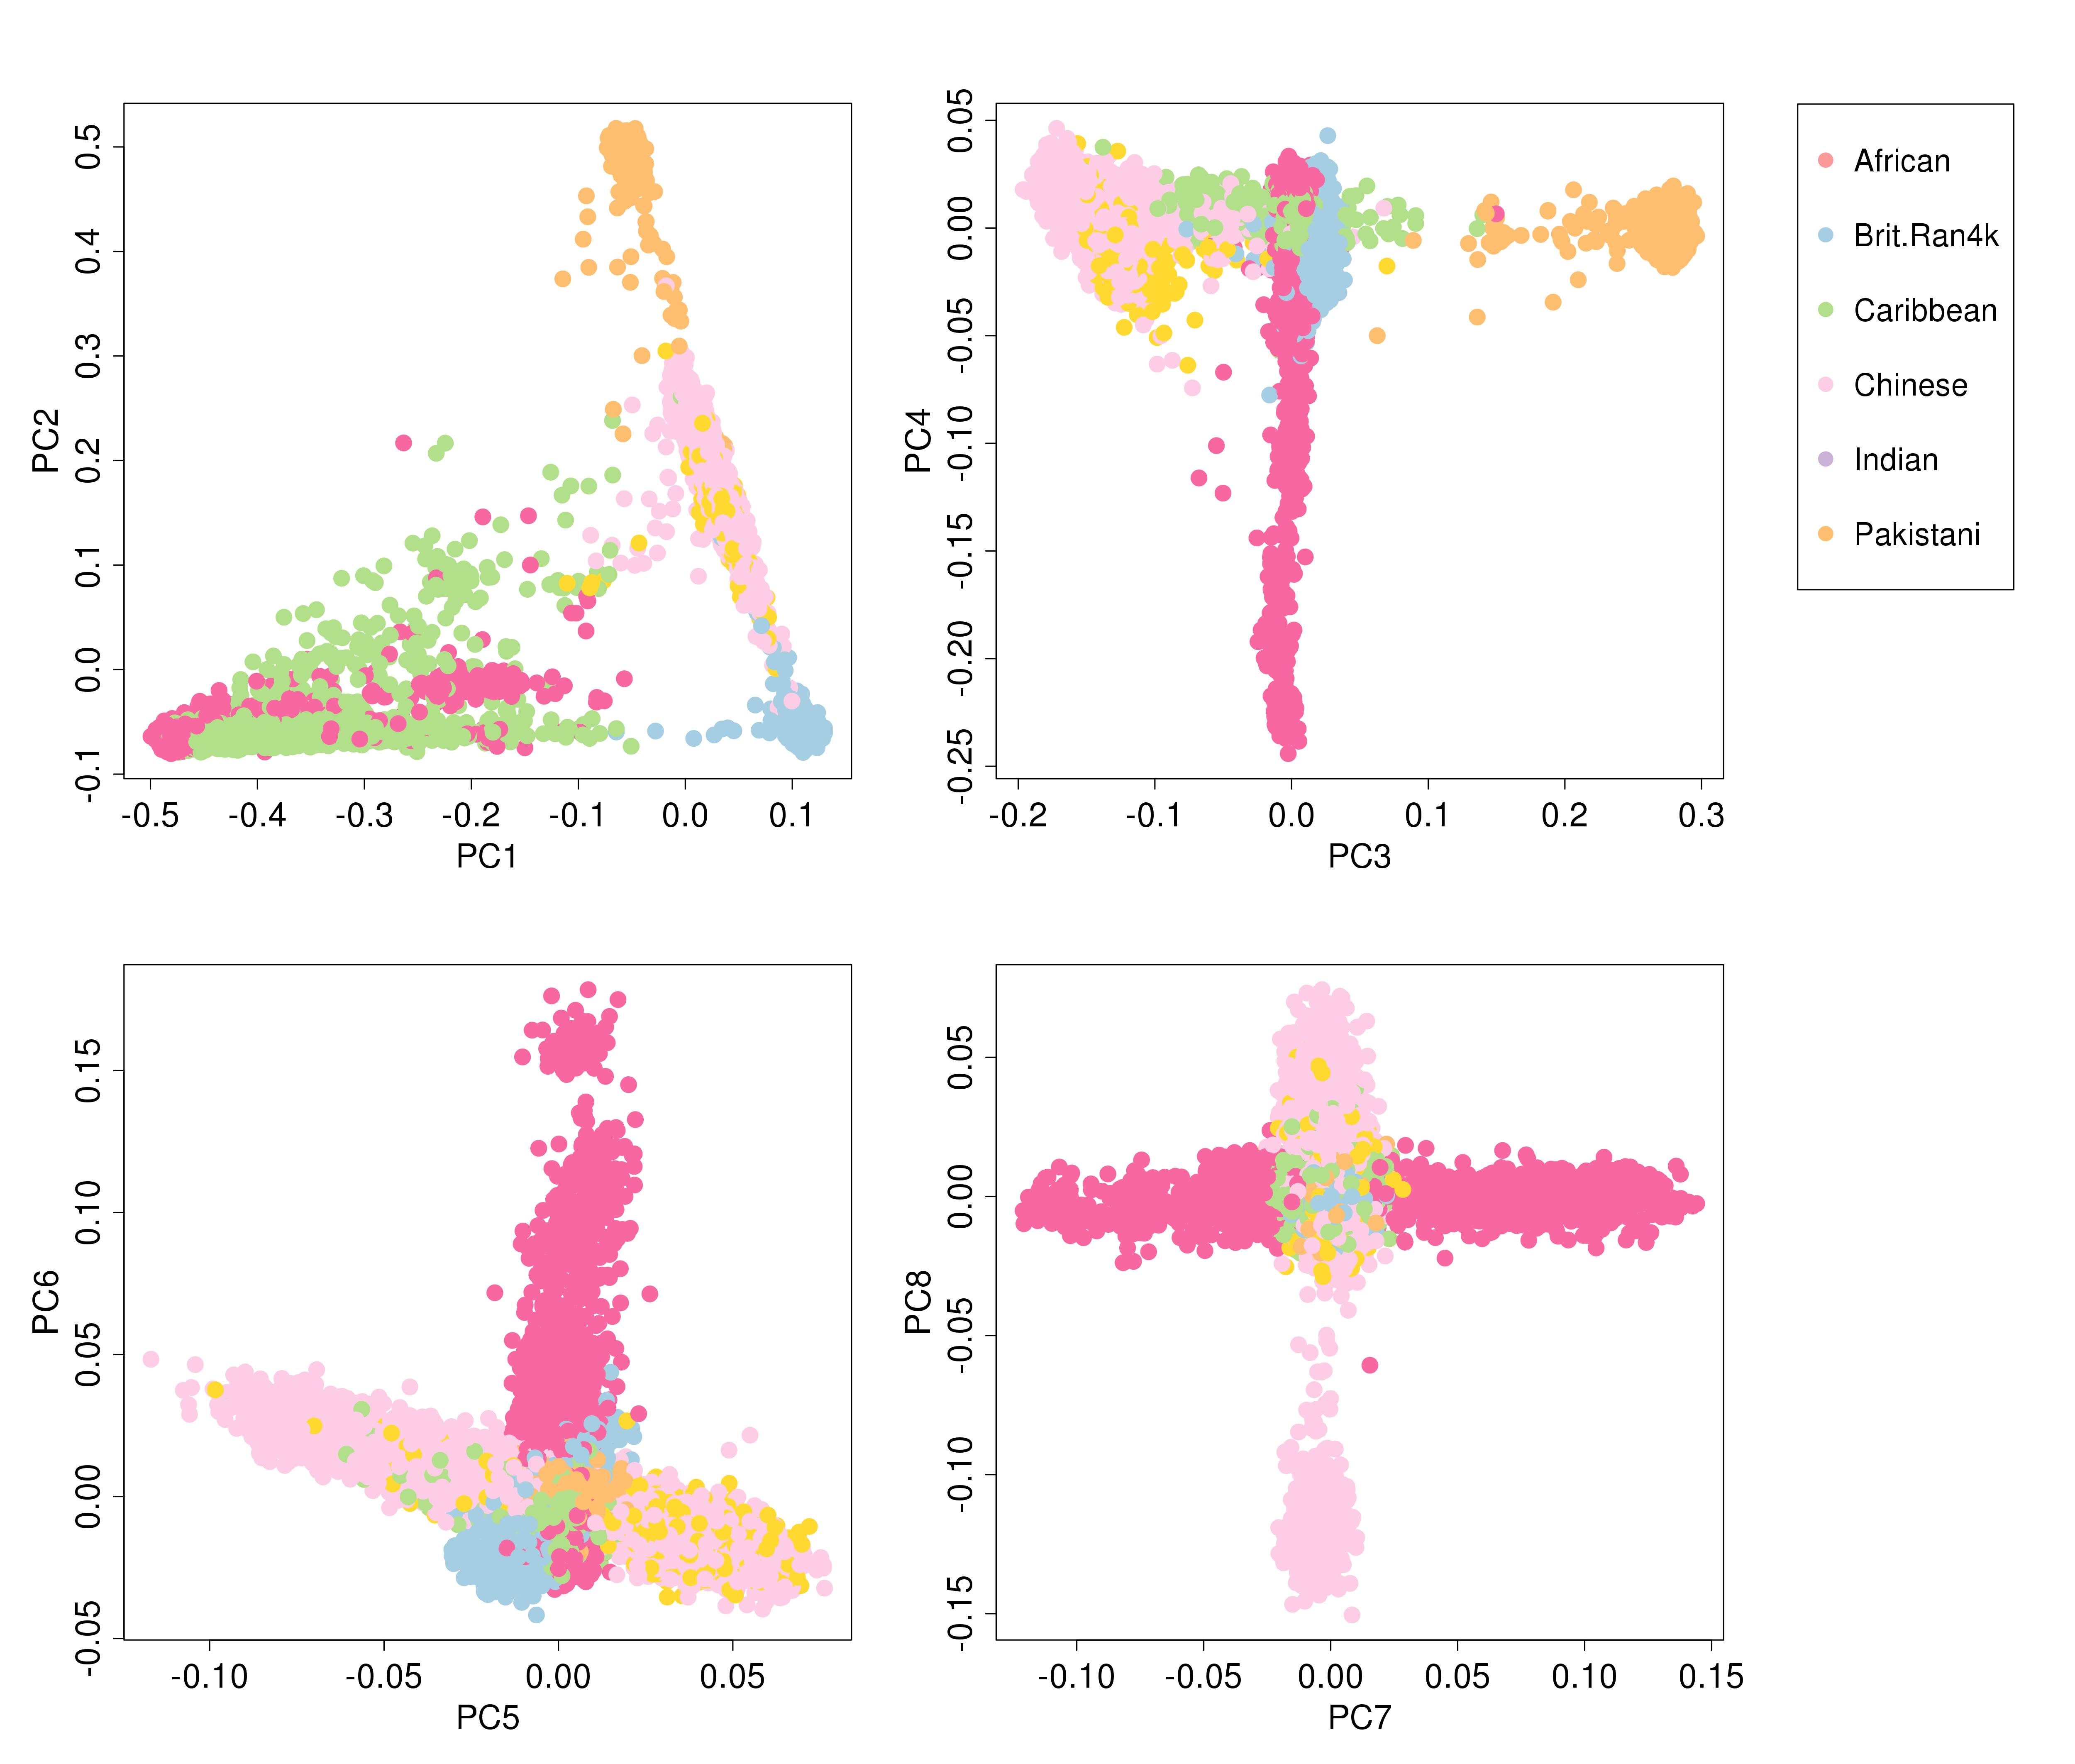
\includegraphics[scale=.4]{Images/Supp/InterPath_Supp_Figure_UKB_PCAPlot_vs1.png}
\caption[TBD]{\textbf{Global PCA Plots of the UK BioBank Subsets}. The figure shows the top 8 global principal components of our UKB subset dataset plotted against one another: a) PC1 vs. PC2, b) PC3 vs. PC4, c) PC5 vs. PC6, d) PC7 vs. PC8. PCA was conducted using FlashPCA \citep{Abraham2017} and a post-QC, pruned SNP set. Note that these PCs were created similar to the descriptions in `Population Subsets' of Methods and `Population Subset Quality Control' of Supplementary Note, but in lieu of running FlashPCA on each subset separately, FlashPCA was run on the full dataset together jointly. Local PCs were used for quality control and as covariates; global PCs were only used for these plots.}
\label{InterPath-Supp-Figure-UKB-Subsets-PCAPlot}
\end{figure}
\clearpage

\begin{figure}[htbp]
\centering
\hspace*{-1.7cm}
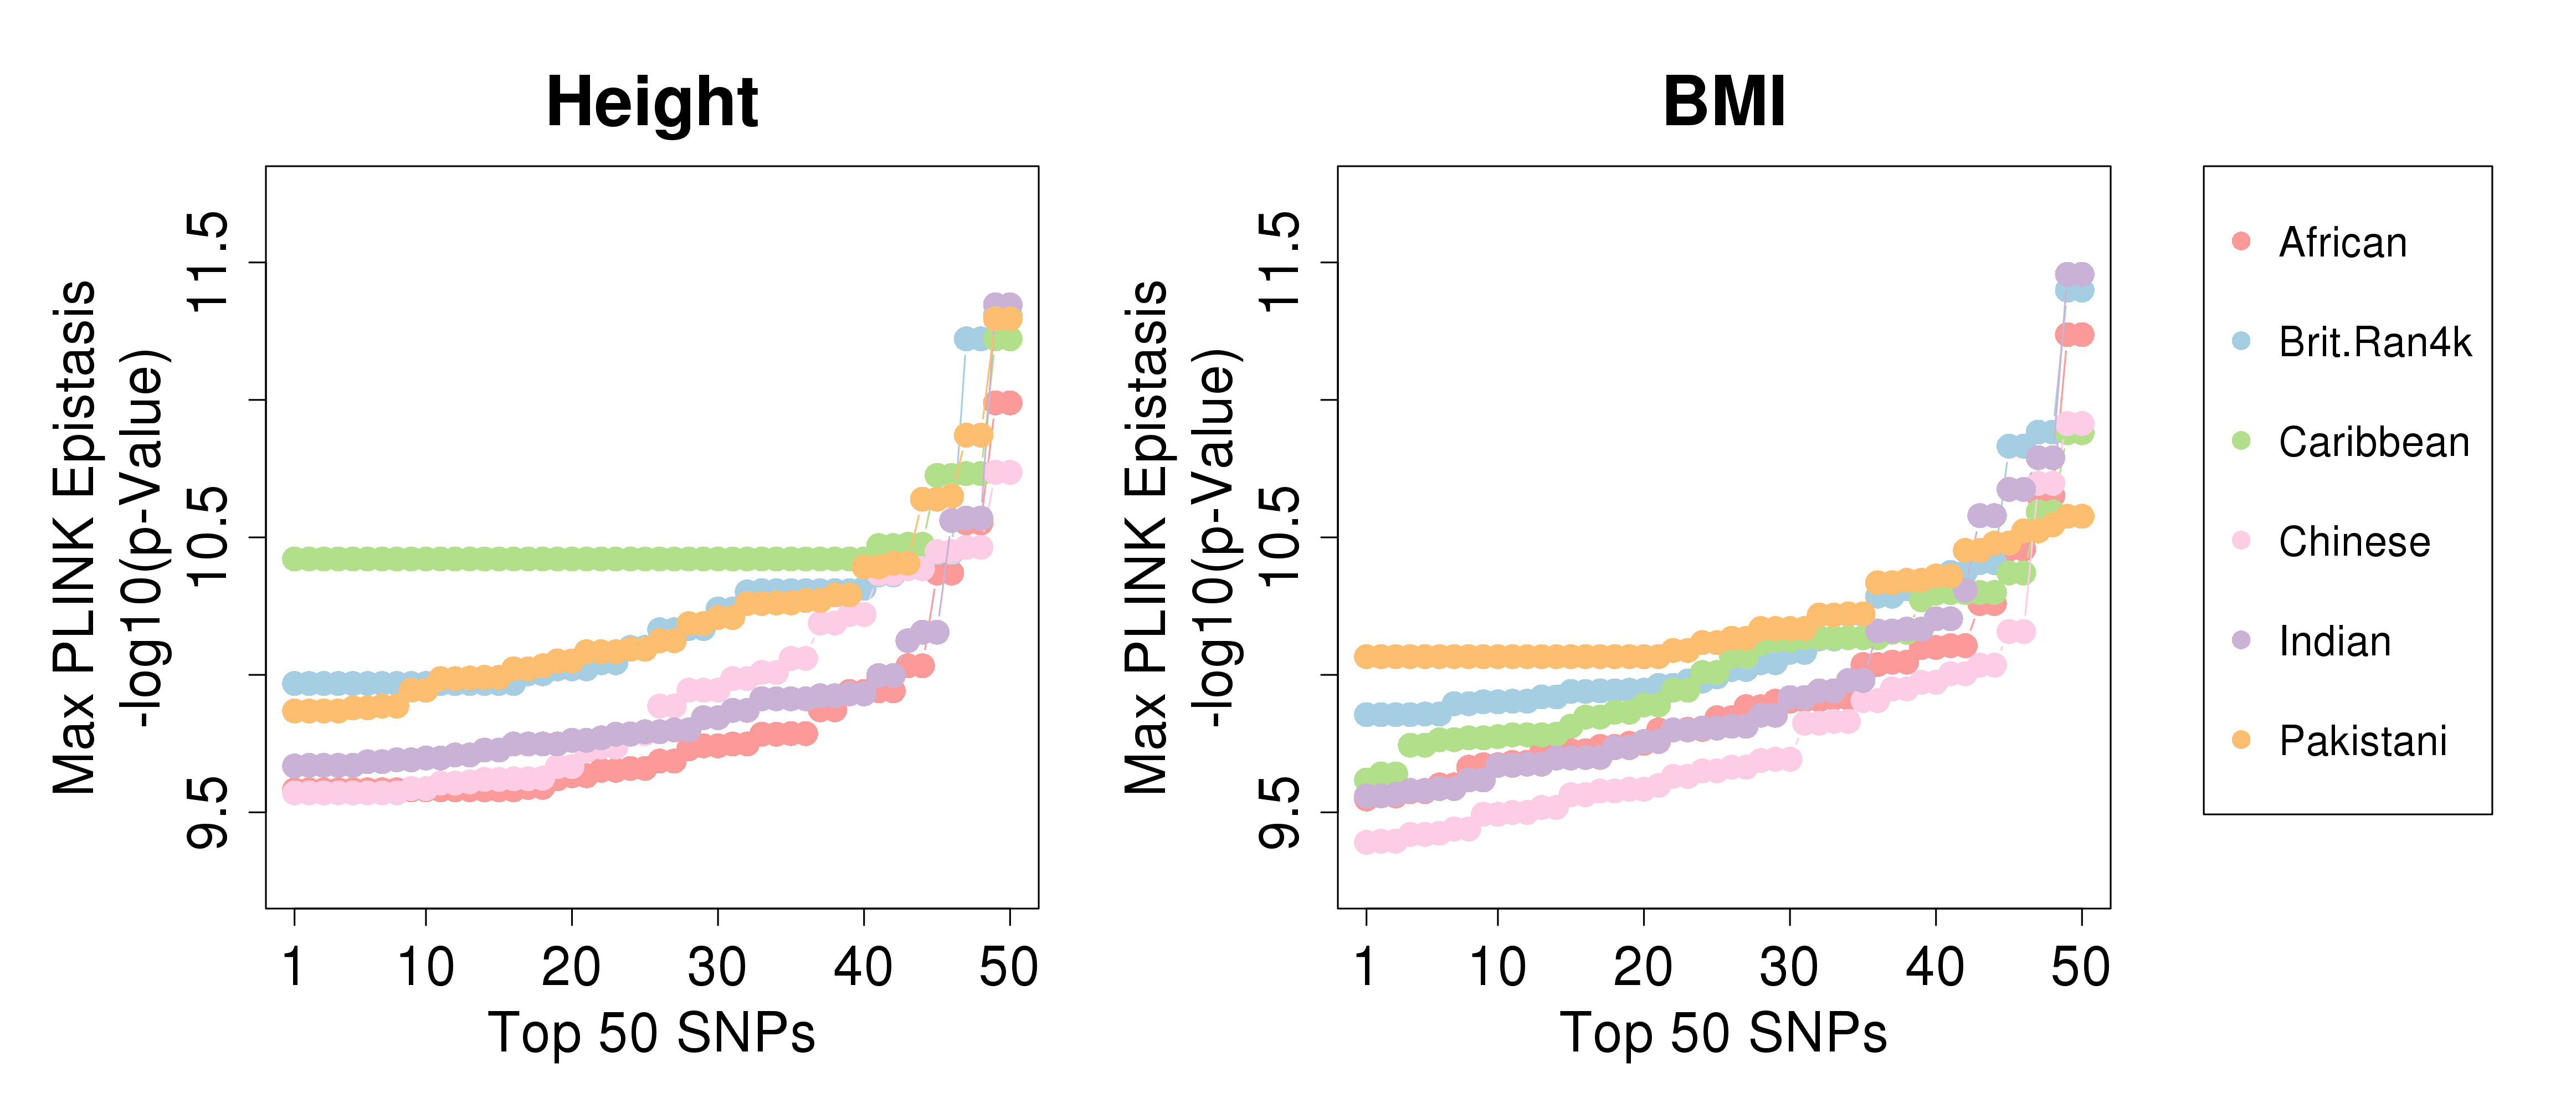
\includegraphics[scale=.45]{Images/Supp/InterPath_Supp_Figure_PLINK_BestSNPs_vs2_AllPops_HeightBMI.png}
\caption[TBD]{\textbf{SNPs with the largest PLINK pairwise epistasis signals, per subset}. The figure shows the best $p$-values obtained from running PLINK's exhaustive pairwise SNP epistasis test for both height and BMI in each of the UKB subsets. Only the top 50 SNPs, sorted by best pairwise SNP epistasis $p$-value, for each subset are shown. No test reaches genome-wide significance based on using a Bonferroni-corrected $p$-value threshold ($p$-value $<= 5\times10^{-13}$).}
\label{InterPath-Supp-Figure-PLINK-HeightBMI-AllPops}
\end{figure}
\clearpage

%\begin{figure}[htbp]
%\centering
%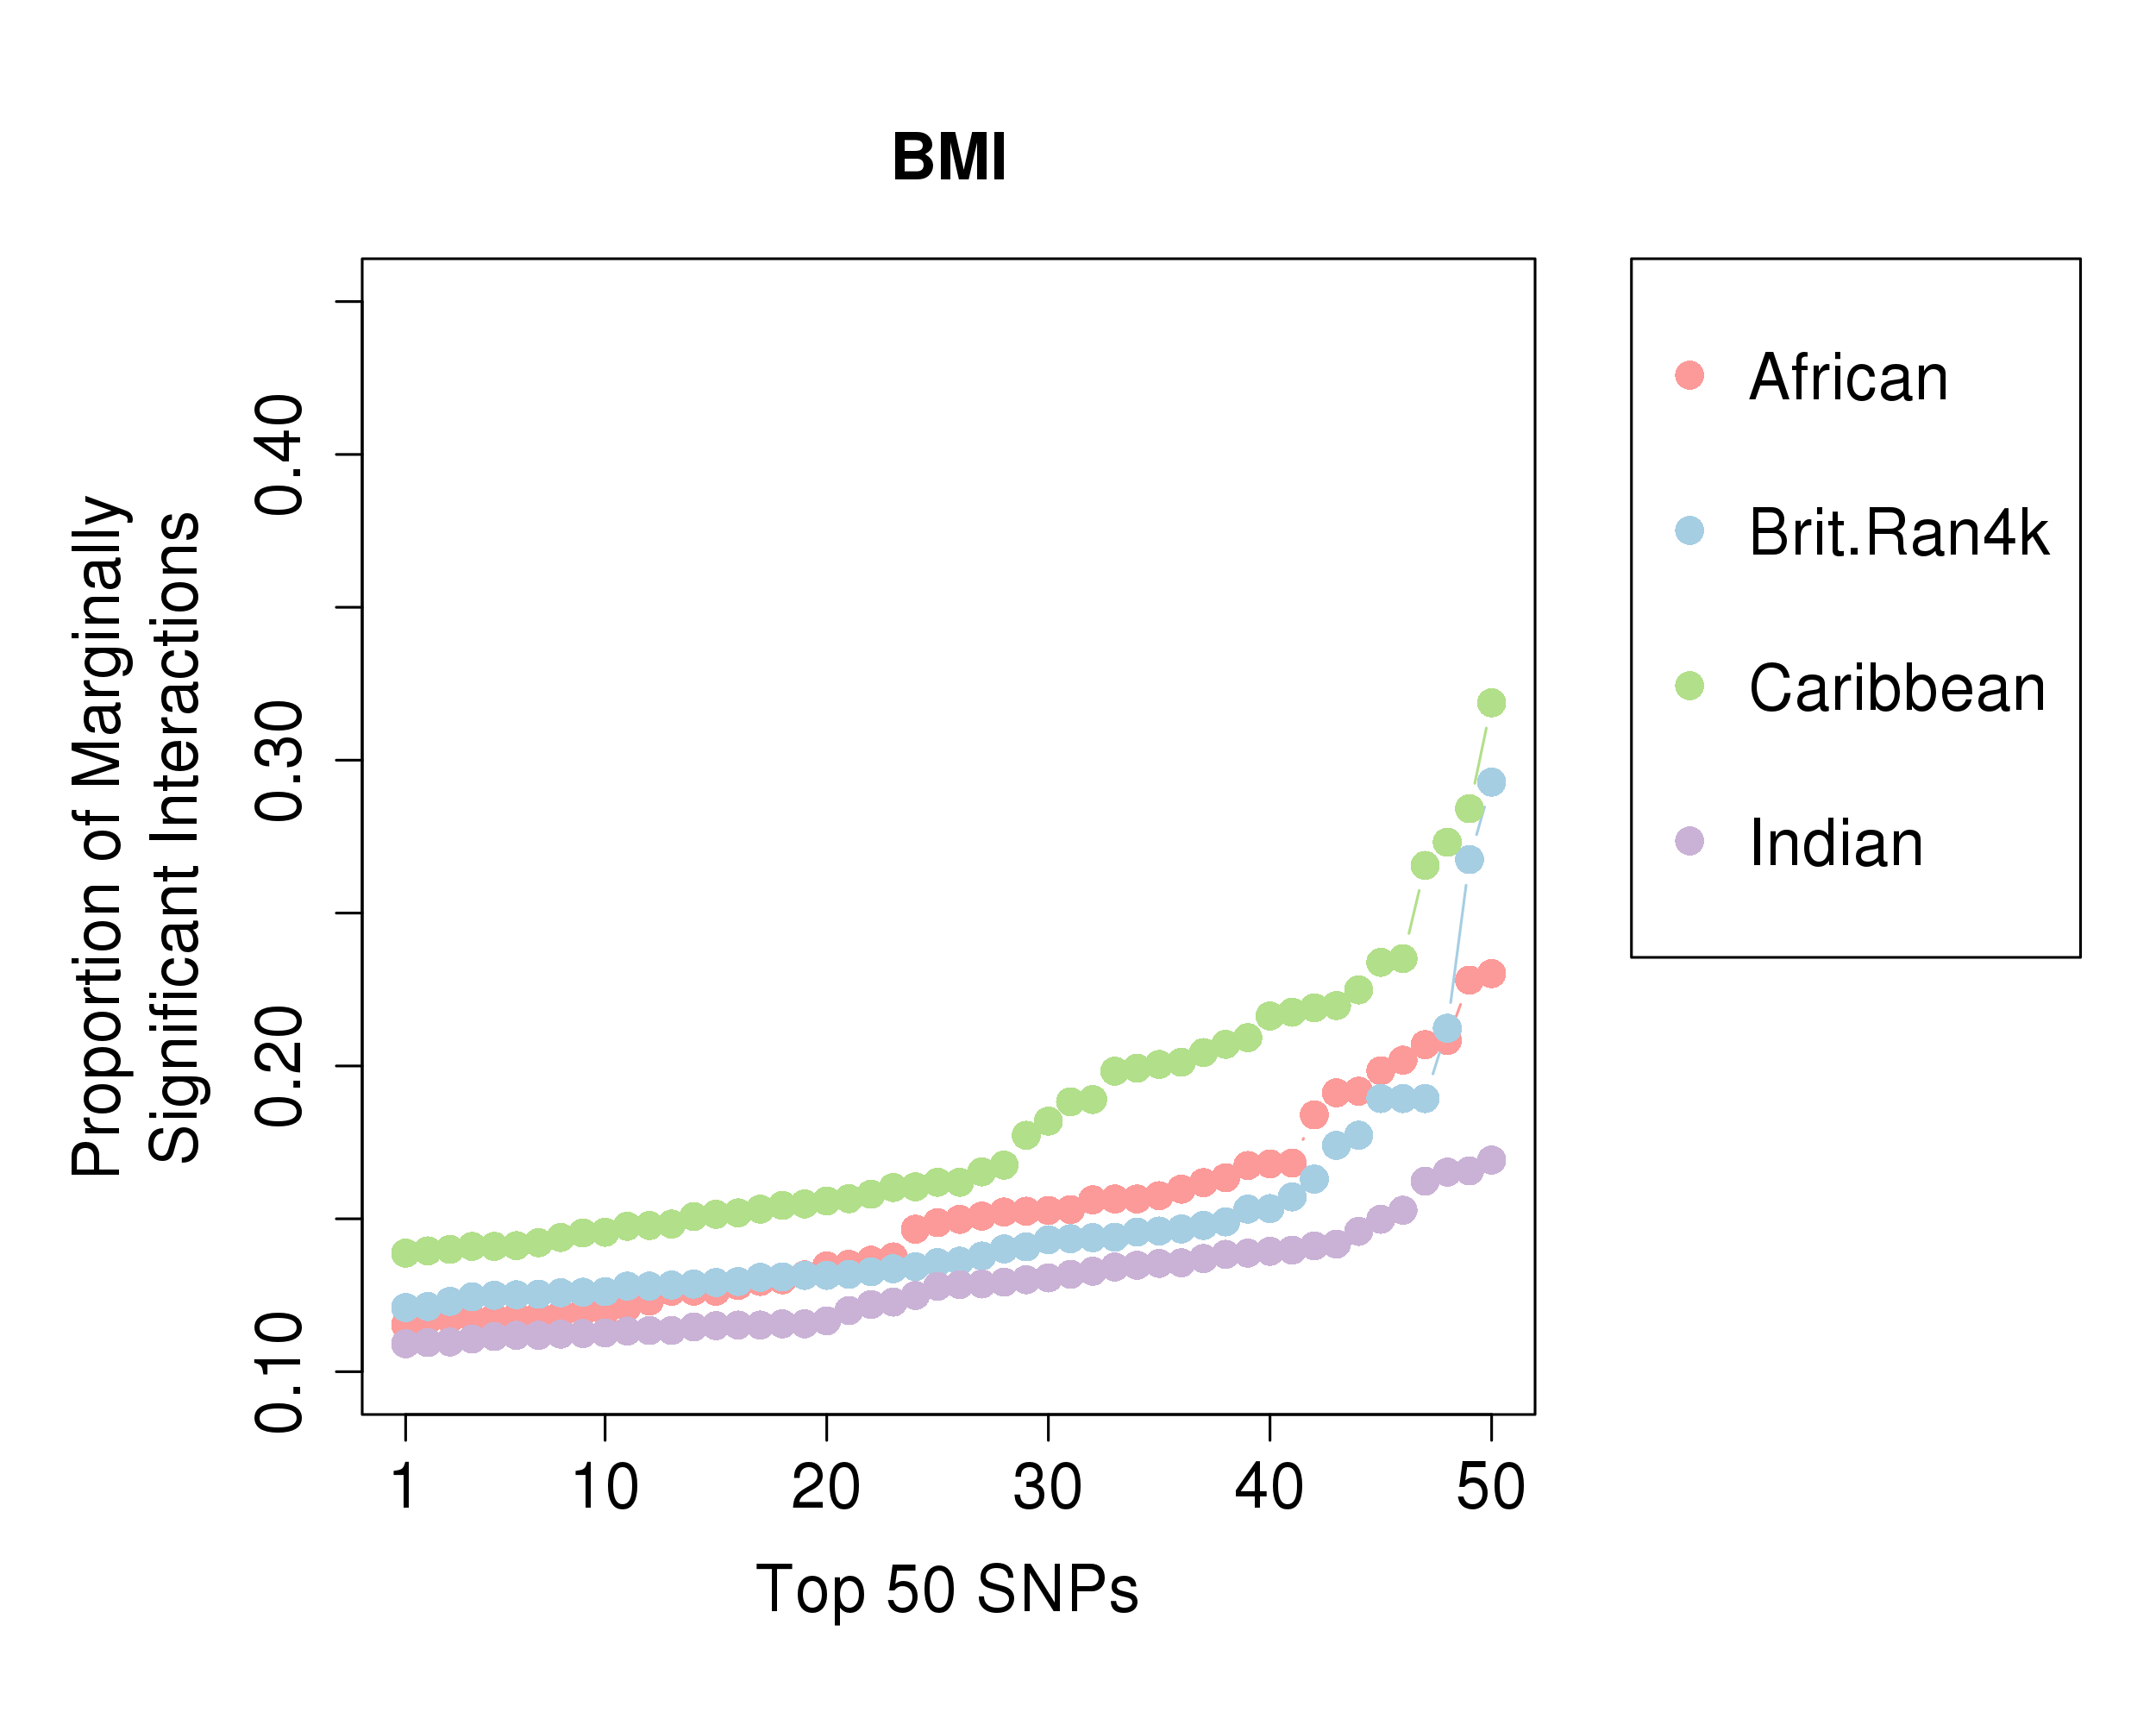
\includegraphics[scale=.5]{Images/Supp/InterPath_Supp_Figure_PLINK_vs3_BMI.png}
%\caption[TBD]{\textbf{PLINK Epistasis Proportion Results: BMI}. The figure shows the proportion of pairwise marginally significant epistatic interactions a single SNP contains when tested on height within our UKB subsets. Pairwise tests are conducted exhaustively for each individual SNP through PLINK. Marginally significant is defined as pairwise SNP epistasis $p$-value $<= 1\times10^{-4}$. Only the top 50 SNPs sorted by decreasing proportion are shown for each UKB subset. For results on height see Figure \ref{InterPath-Main-Figure-PLINK-Proportions-Height}. In general we find that the African and Caribbean subsets have the highest proportions of marginally significant interactions per SNP.}
%\label{InterPath-Supp-Figure-PLINK-Proportions-BMI}
%\end{figure}

\begin{figure}[htb]
\centering
\hspace*{-1.7cm}
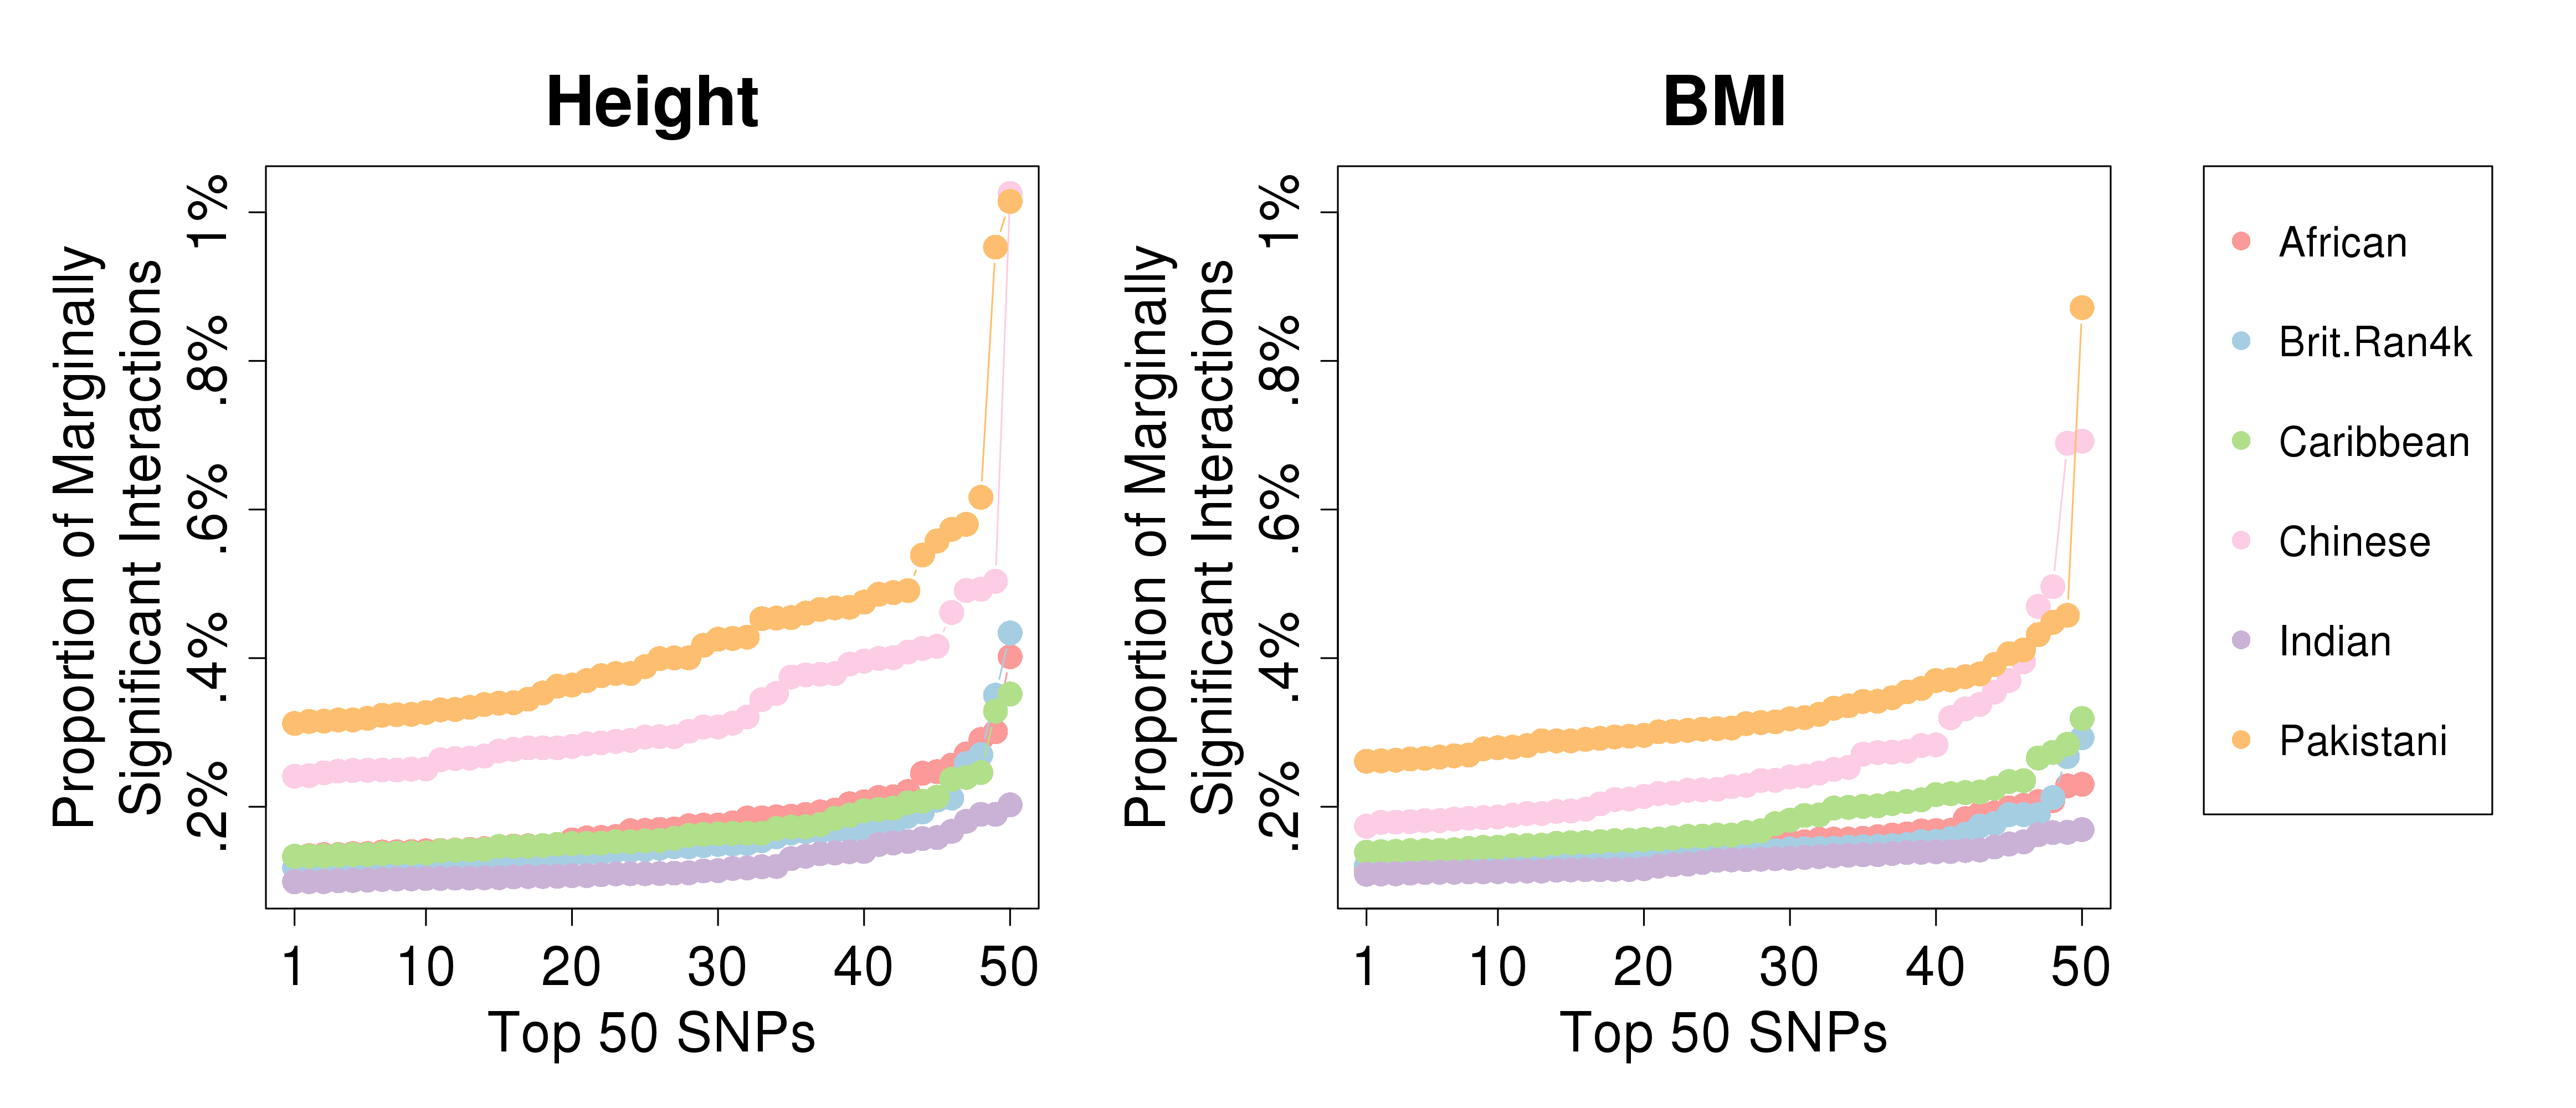
\includegraphics[scale=.45]{Images/Main/InterPath_Main_Figure_PLINK_vs4_HeightBMI.png}
\caption[TBD]{\textbf{SNPs with the largest proportions of marginally significant PLINK pairwise epistasis tests, per subset}. The figure shows the proportion of pairwise marginally significant epistatic interactions a single SNP contains when tested on height and BMI within our UKB subsets. Pairwise tests are conducted exhaustively for each individual SNP through PLINK. Marginally significant is defined as a pairwise SNP epistasis $p$-value $<= 1\times10^{-4}$. Only the top 50 SNPs sorted by decreasing proportion are shown for each UKB subset. In general we find that the African and Caribbean subsets have the highest proportions of marginally significant interactions per SNP.}
\label{InterPath-Supp-Figure-PLINK-Proportions-HeightBMI}
\end{figure}

%\begin{figure}[htbp]
%\centering
%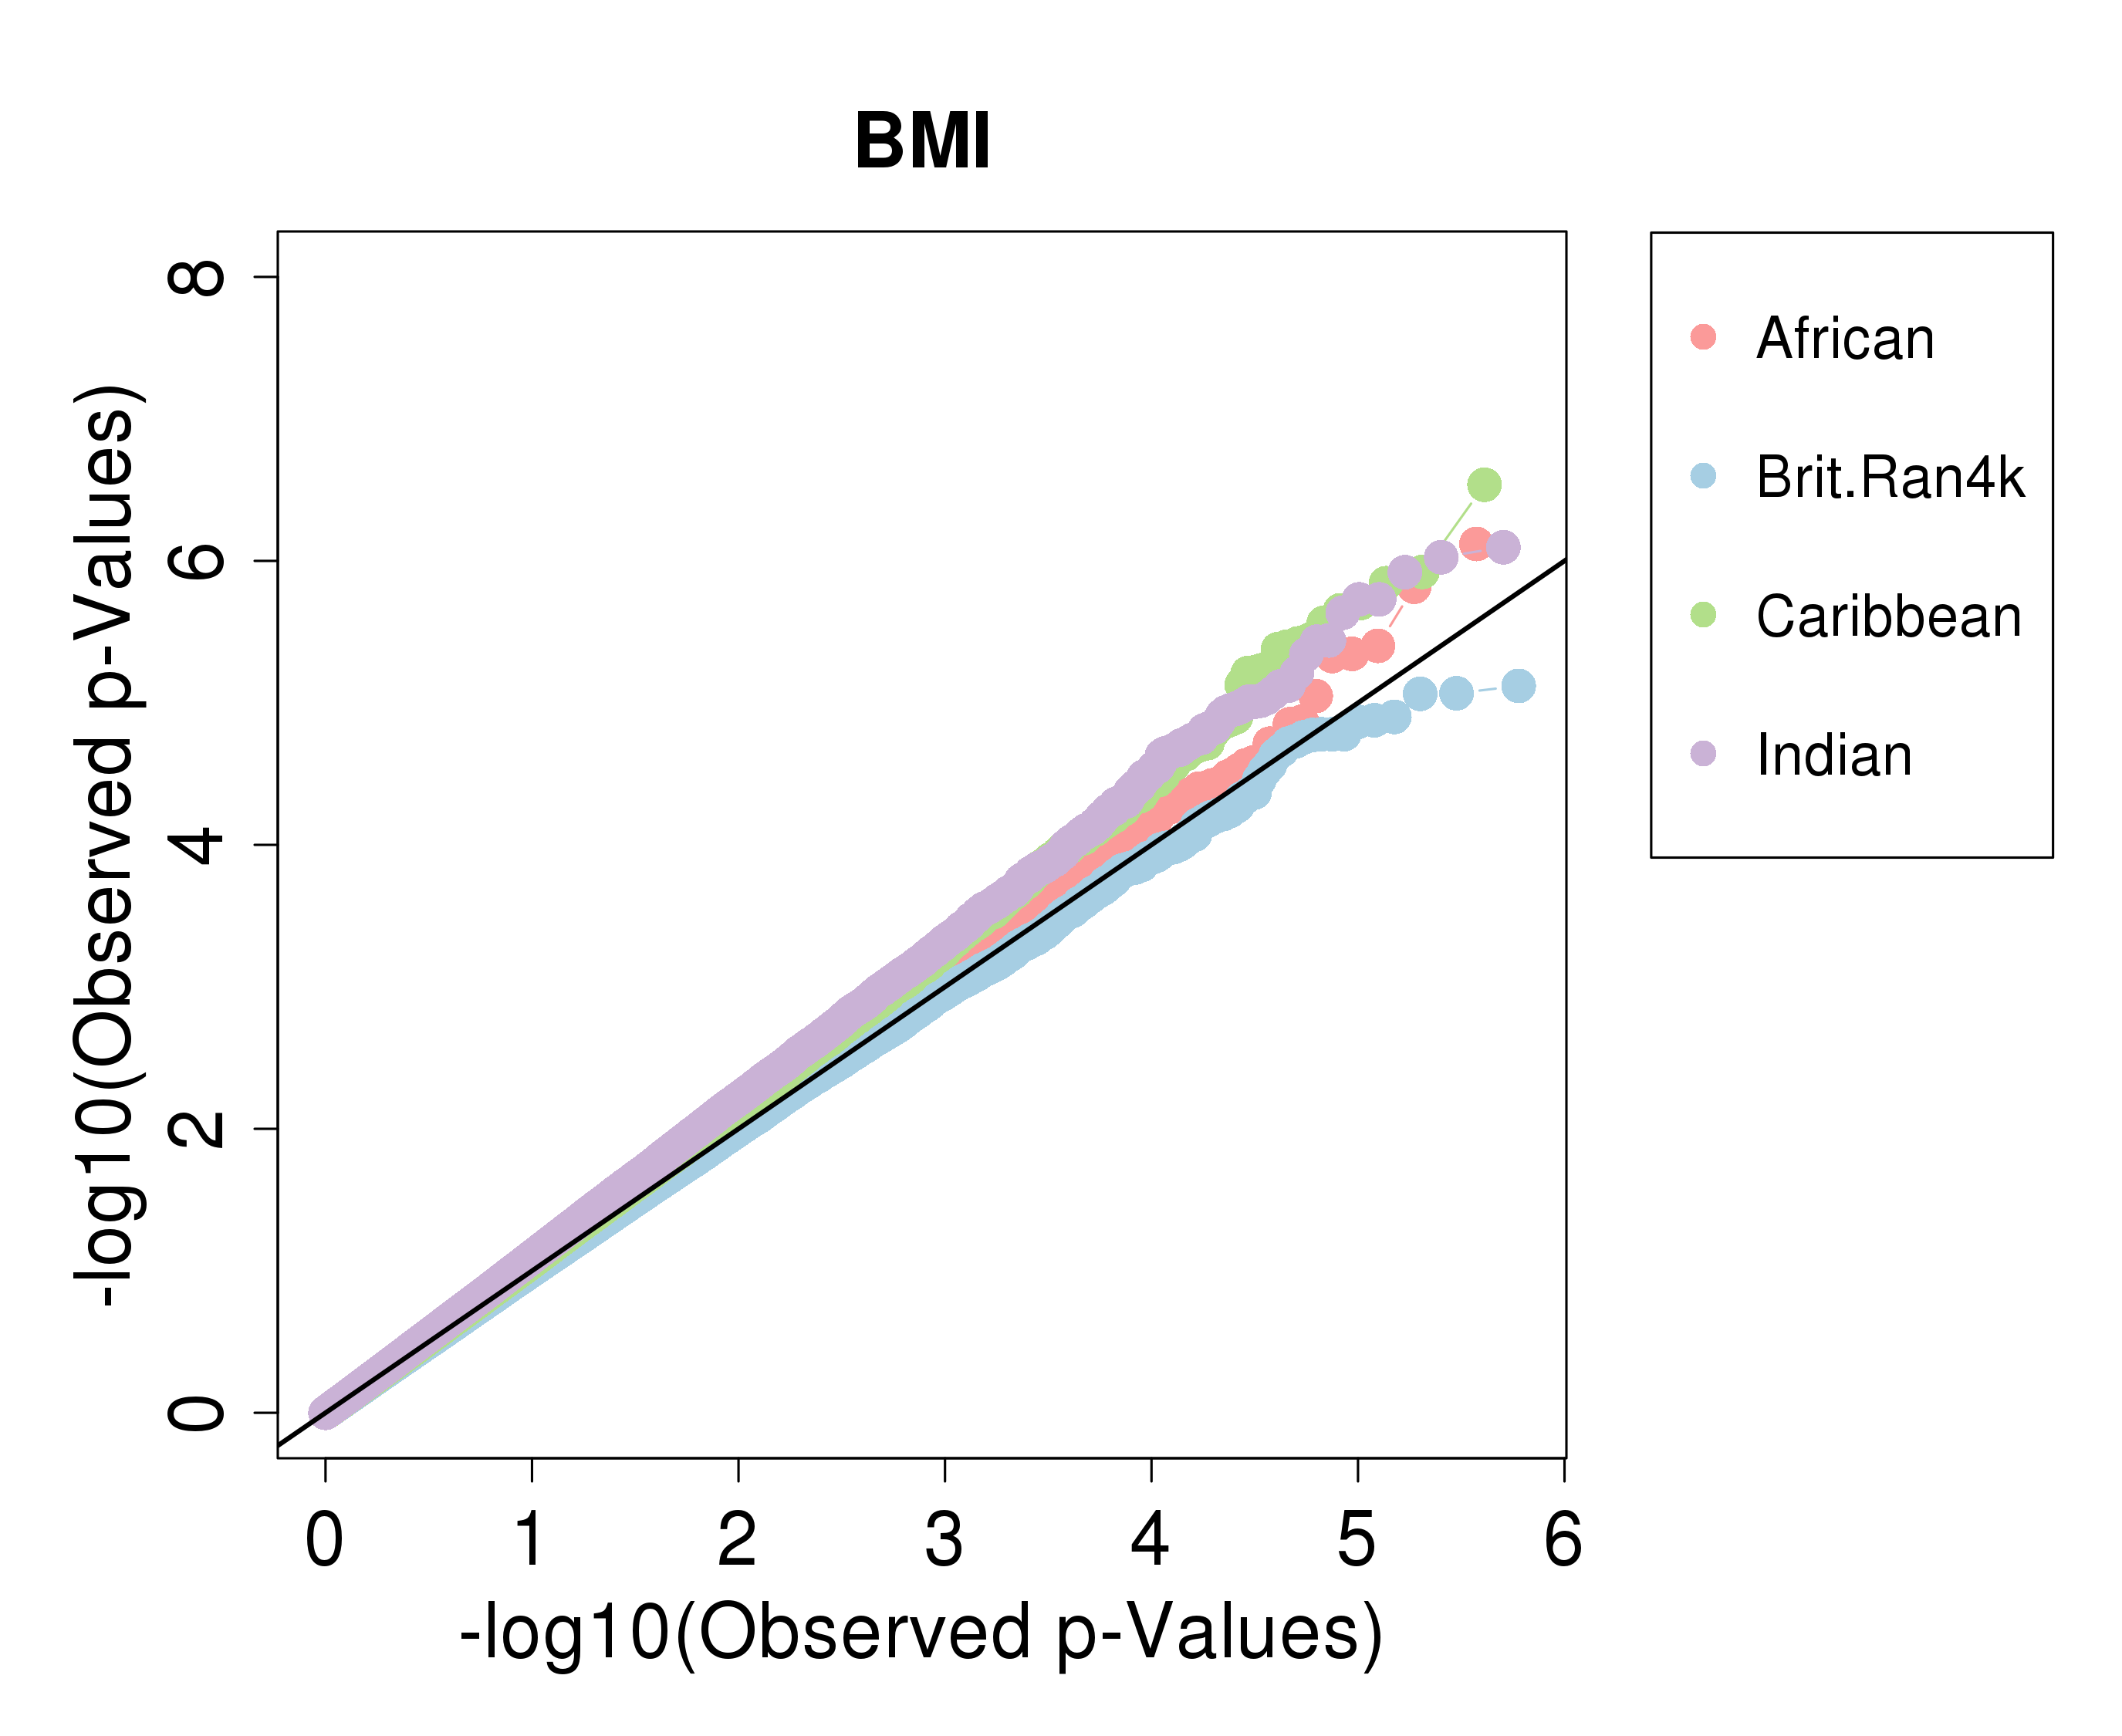
\includegraphics[scale=.5]{Images/Supp/InterPath_Supp_Figure_MAPIT_vs3_BMI.png}
%\caption[TBD]{\textbf{MAPIT Results: BMI QQ-Plots}. The figure shows QQ-plots of our results from running MAPIT on our four initial UKB population subsets in BMI. On the $x$-axis are the -$\log_{10}$ of the expected $p$-values and the on the $y$-axis are on the -$\log_{10}$ of the observed $p$-values. Each data point is a SNP and total SNP counts per UKB subset can be found in Supplementary Table \ref{InterPath-Supp-Table-UKBPopStats}.}
%\label{InterPath-Supp-Figure-MAPIT-BMI}
%\end{figure}
%\clearpage

\begin{figure}[htb]
\centering
\hspace*{-1.4cm}
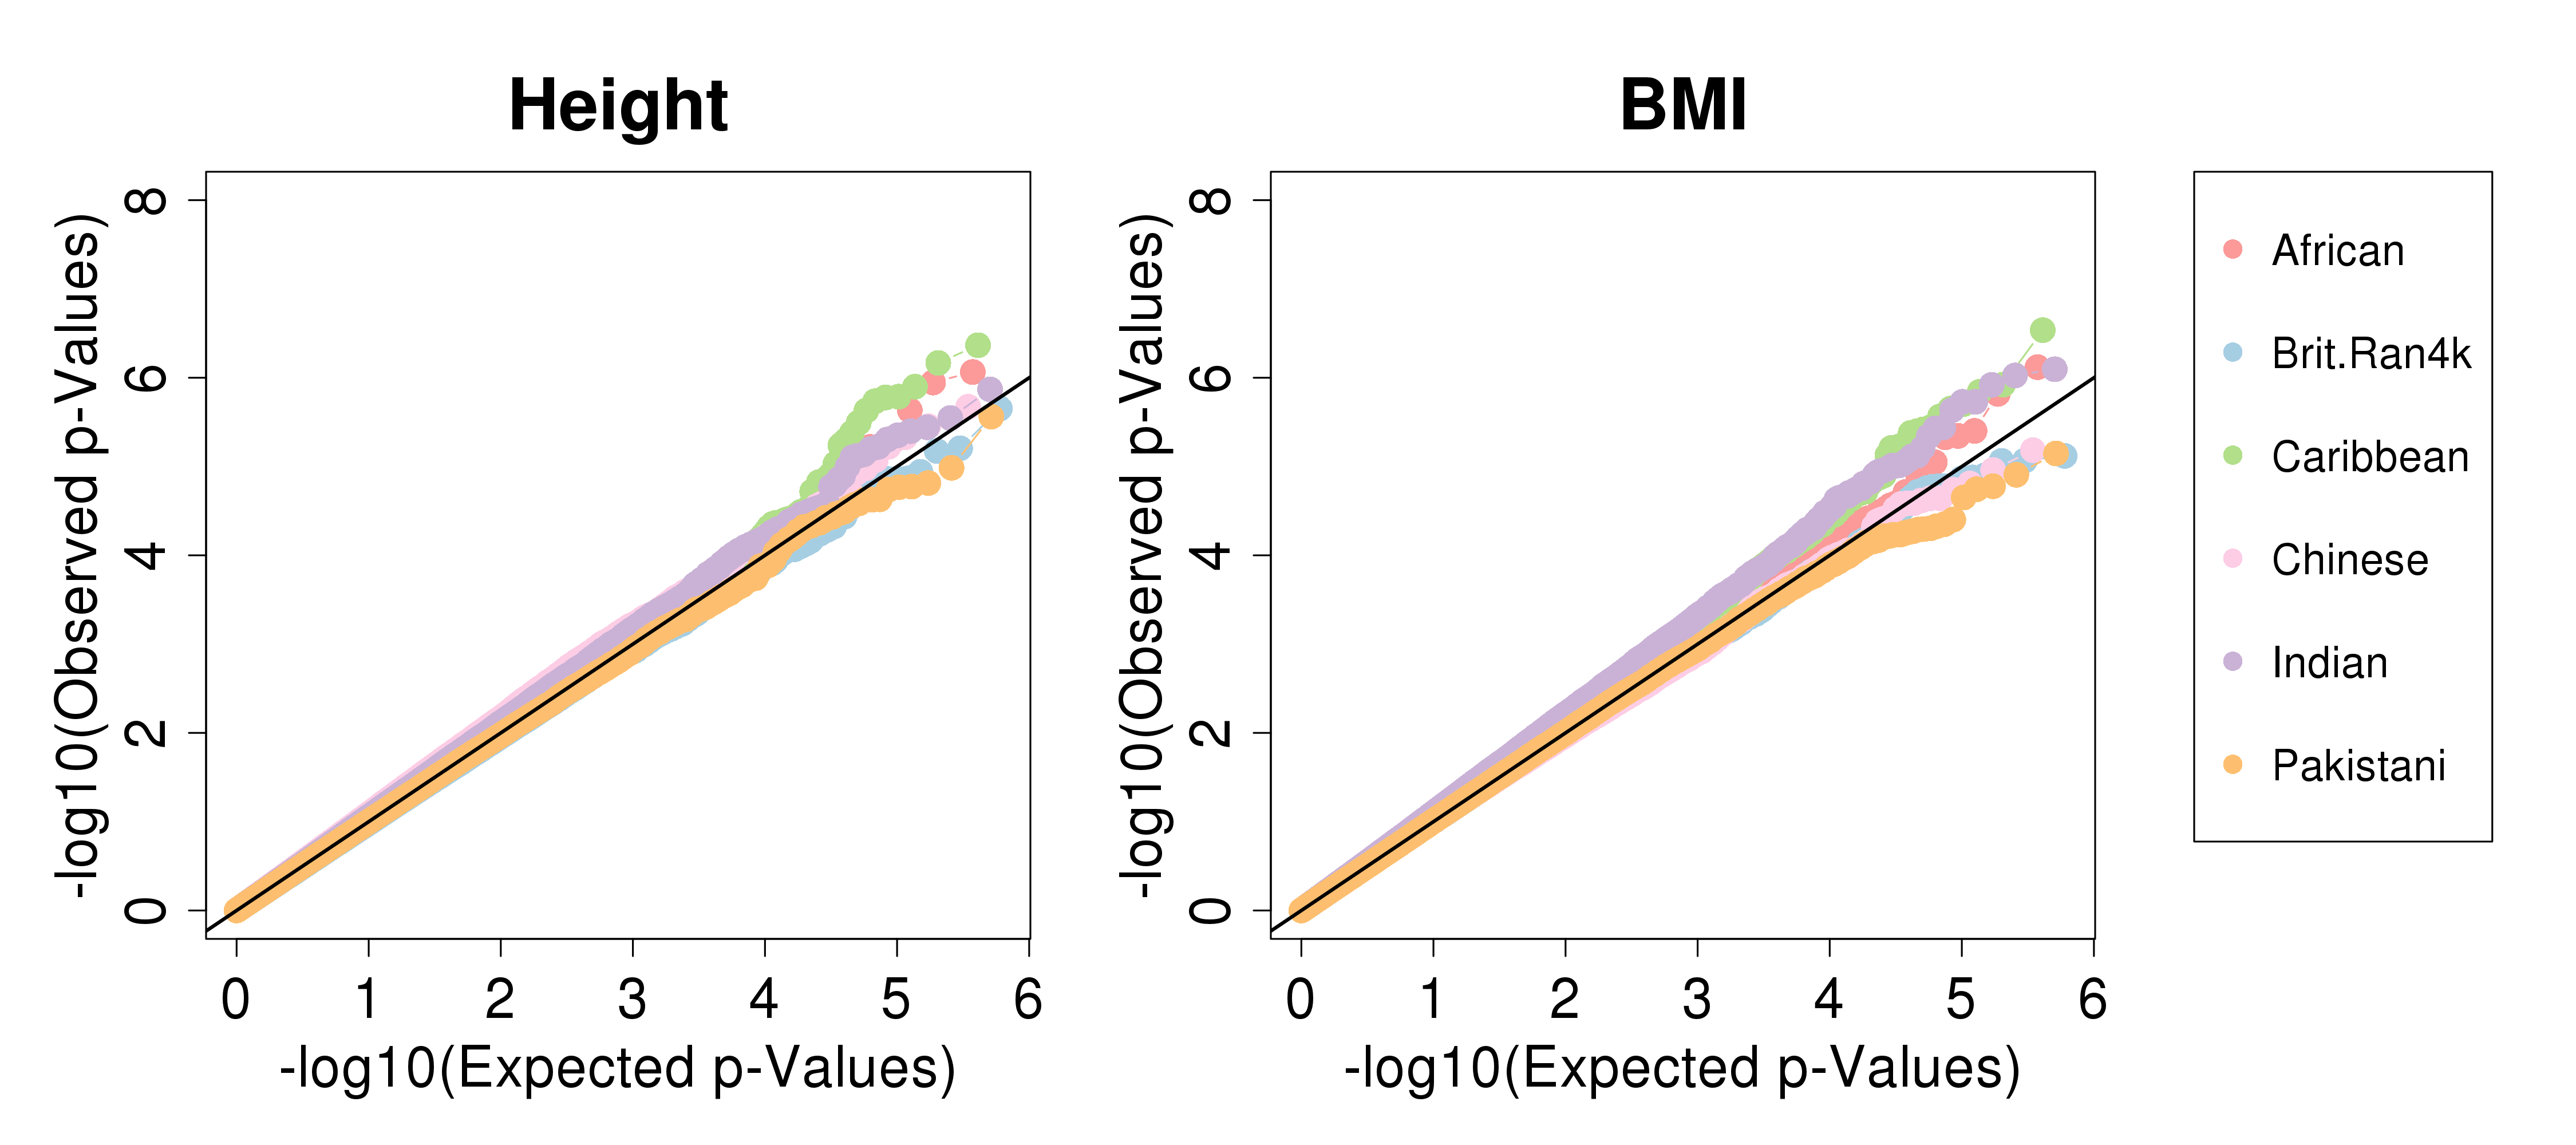
\includegraphics[scale=.45]{Images/Main/InterPath_Main_Figure_MAPIT_vs4_HeightBMI.png}
\caption[TBD]{\textbf{QQ-Plots of MAPIT results, per subset}. The figure shows QQ-plots of our results from running MAPIT on our four initial UKB population subsets in height and BMI. On the $x$-axis are the -$\log_{10}$ of the expected $p$-values and the on the $y$-axis are on the -$\log_{10}$ of the observed $p$-values. Each data point is a SNP and total SNP counts per UKB subset can be found in Supplementary Table \ref{InterPath-Supp-Table-UKBPopStats}. We observe no genome-wide significant signals in any subset across both phenotypes ($p$-value $<= 5\times10^{-8}$) and, due to this lack of significant results, observe no clear differences in patterns between our subsets.}
\label{InterPath-Supp-Figure-MAPIT-HeightBMI}
\end{figure}

%\begin{figure}[htbp]
%\centering
%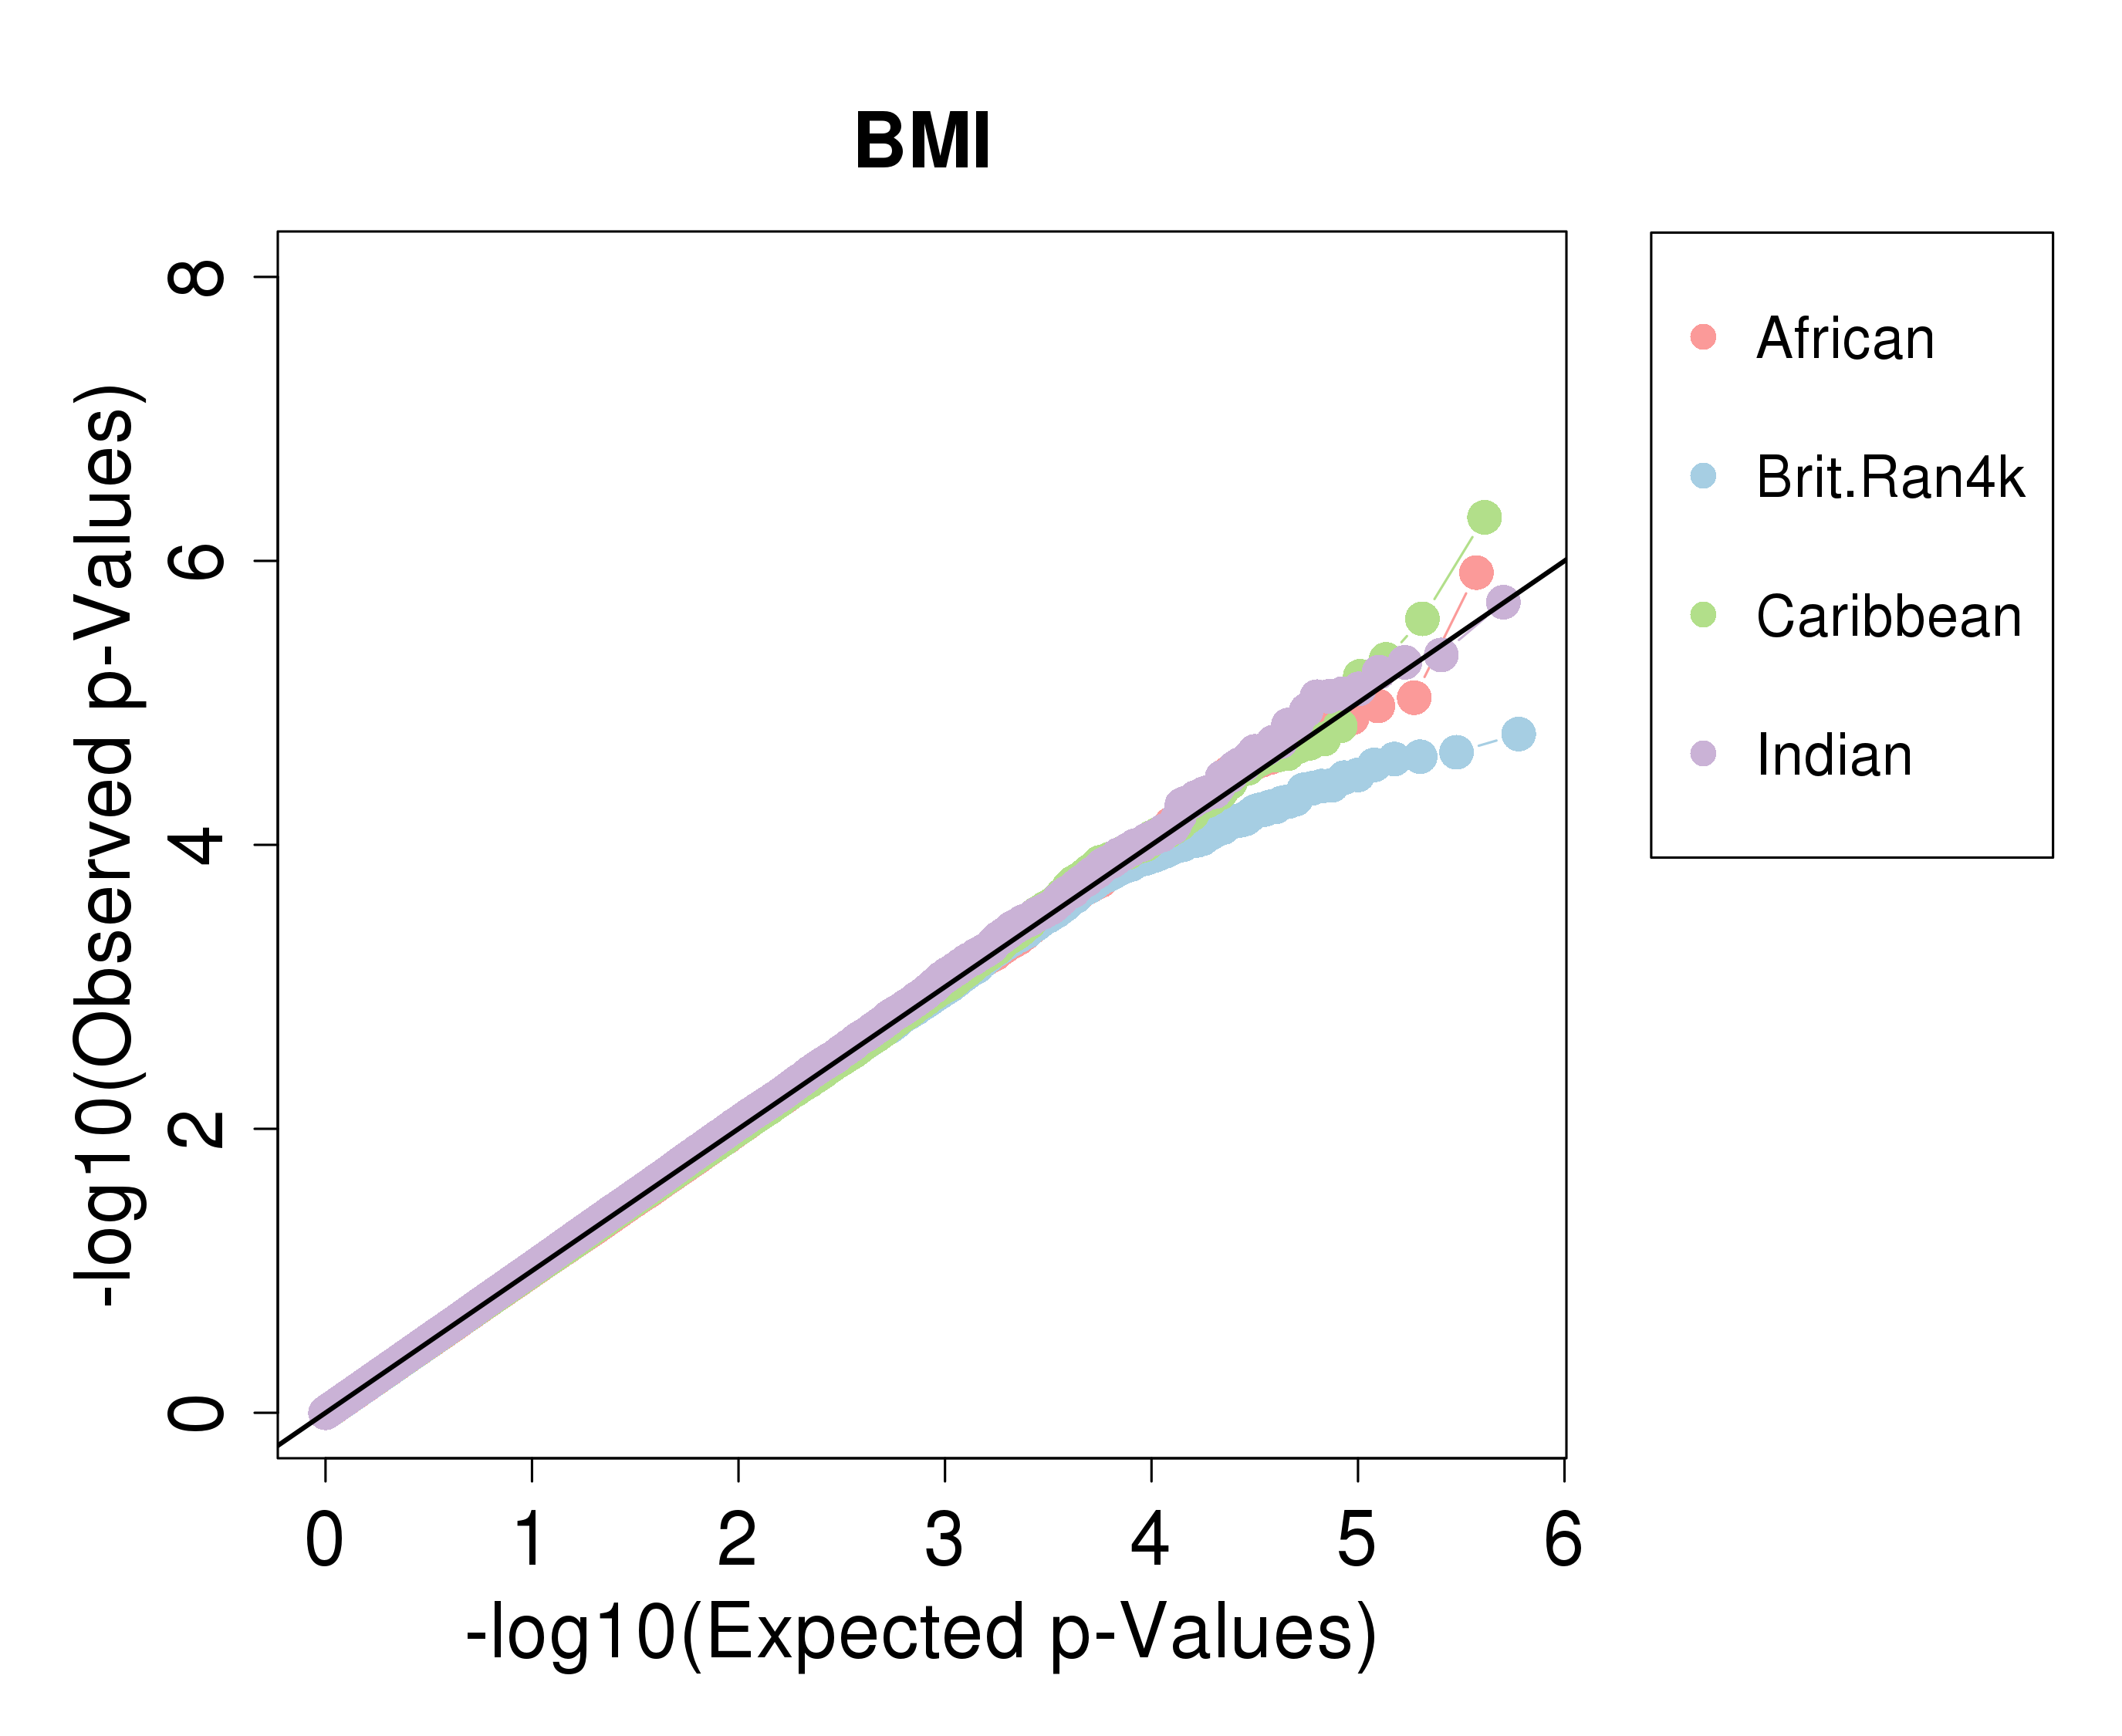
\includegraphics[scale=.35]{Images/Supp/InterPath_Supp_Figure_GWAS_vs2_BMI.png}
%\caption[TBD]{\textbf{GWAS Results QQ-Plots}.}
%\label{InterPath-Supp-Figure-GWAS-BMI}
%\end{figure}
%\clearpage
%
%\begin{figure}[htbp]
%\centering
%\hspace*{-.75cm}
%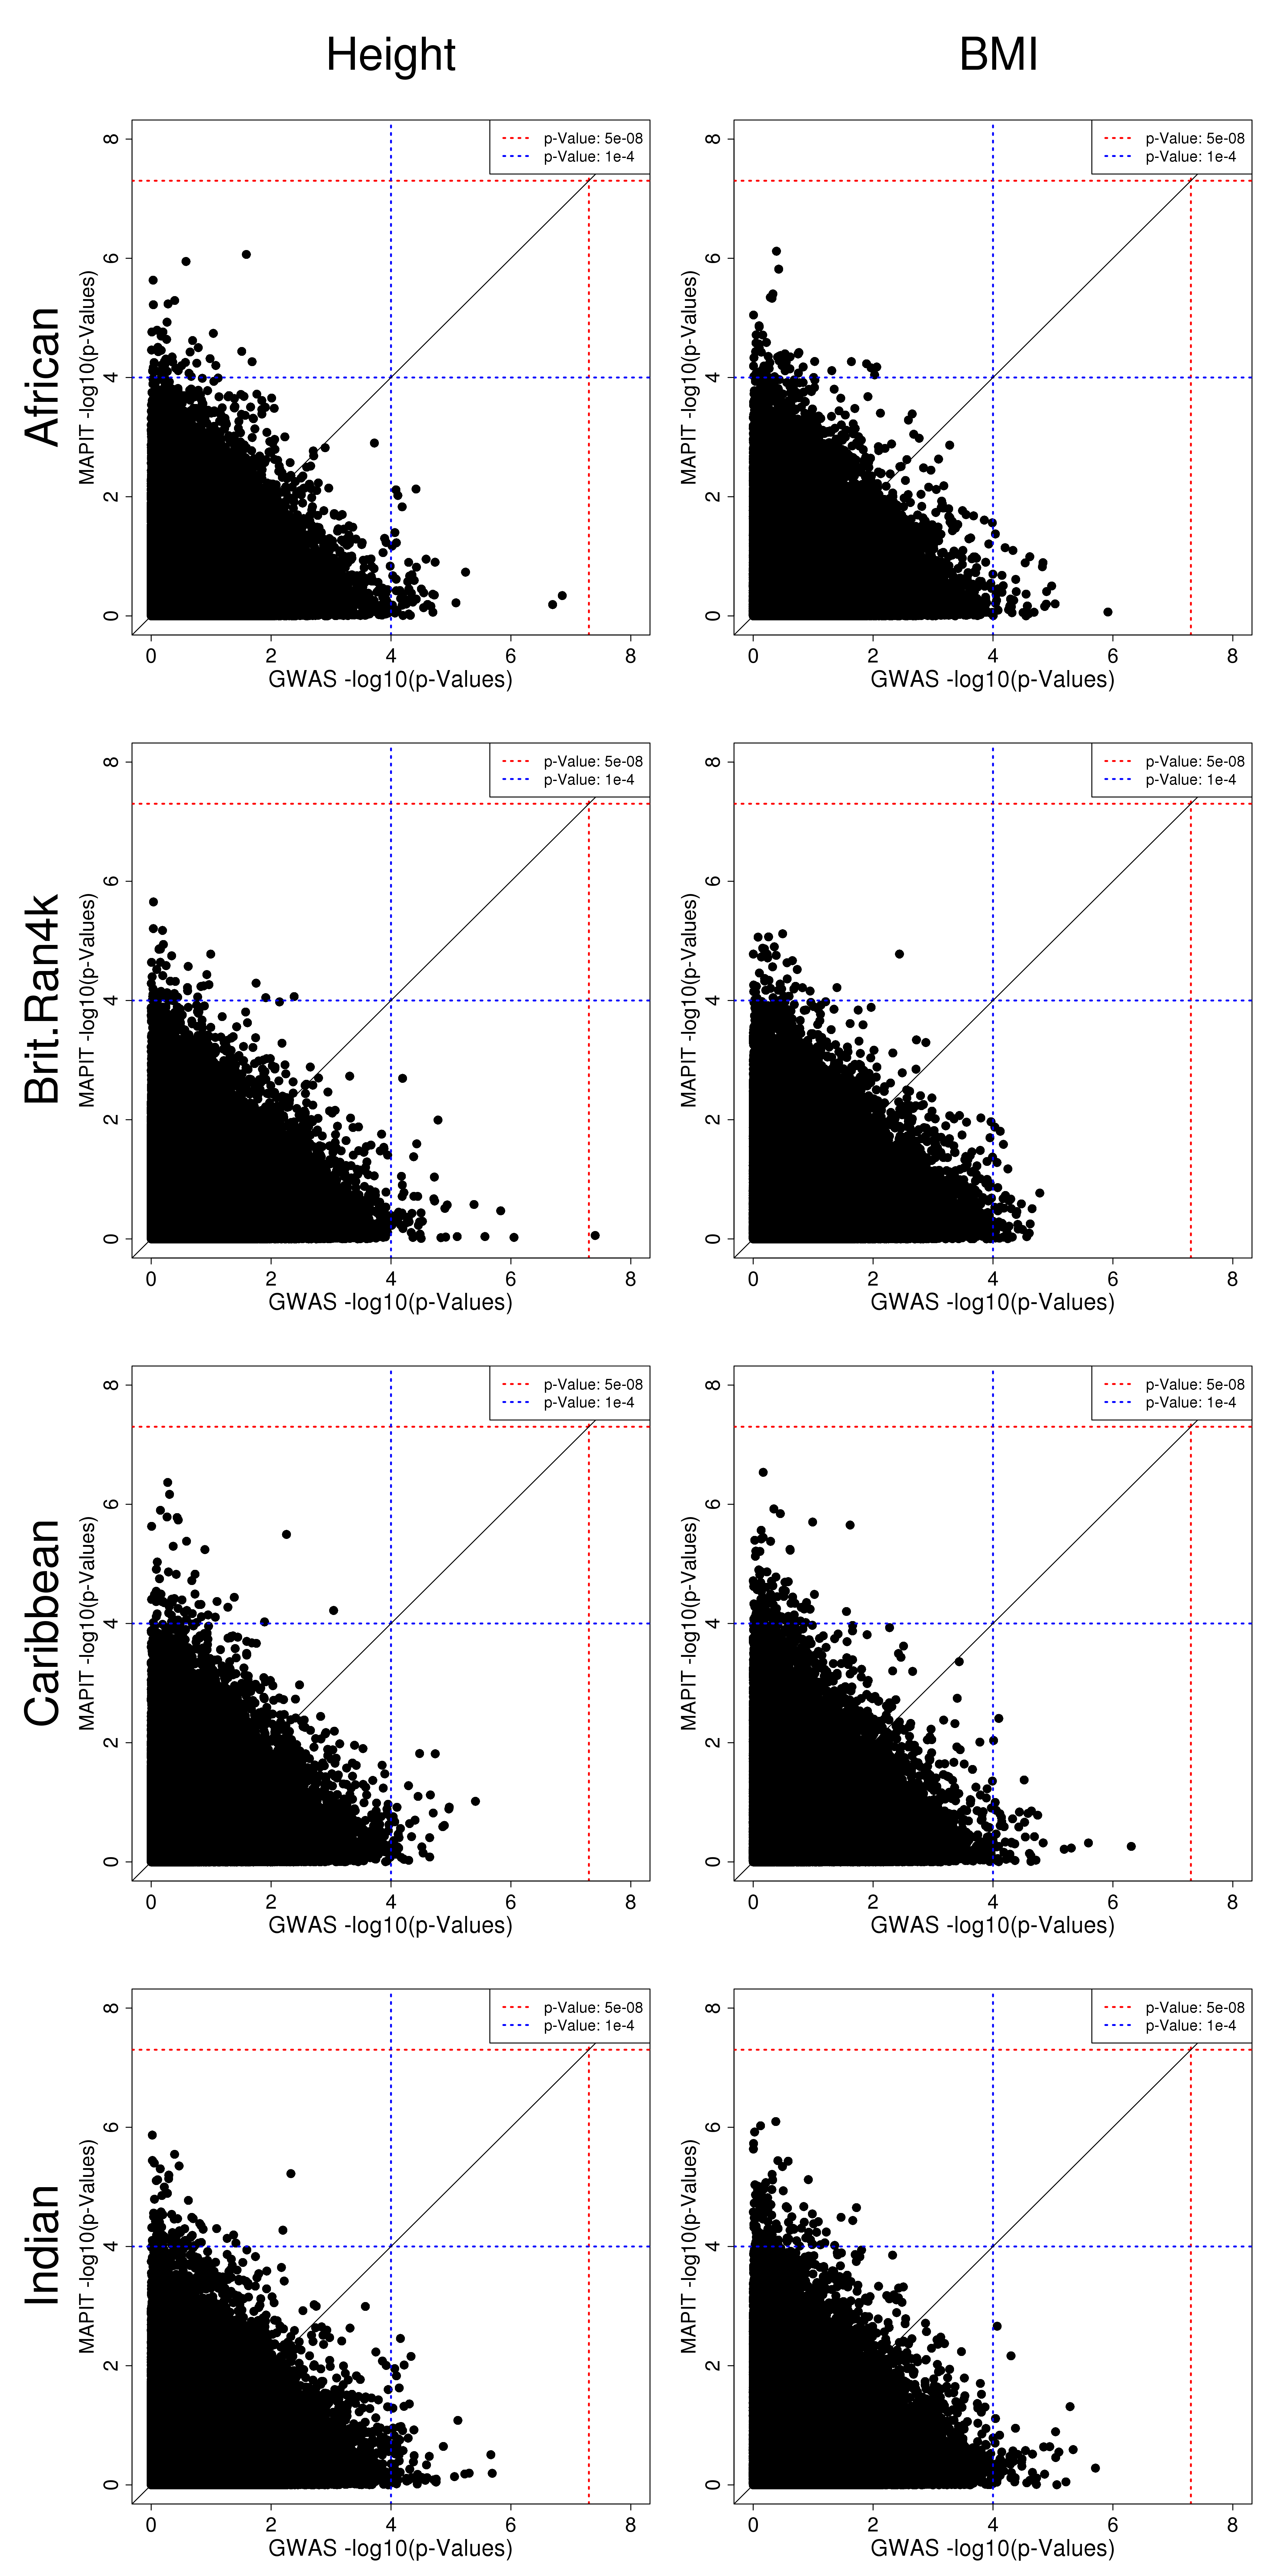
\includegraphics[scale=.3]{Images/Supp/InterPath_Supp_Figure_MAPITvsGWAS_vs2.png}
%\caption[TBD]{\textbf{MAPIT vs. GWAS Results}.}
%\label{InterPath-Supp-Figure-MAPITvsGWAS}
%\end{figure}
%\clearpage

\setlength{\footskip}{3cm}
\begin{figure}[htbp]
\centering
\vspace*{-2cm}
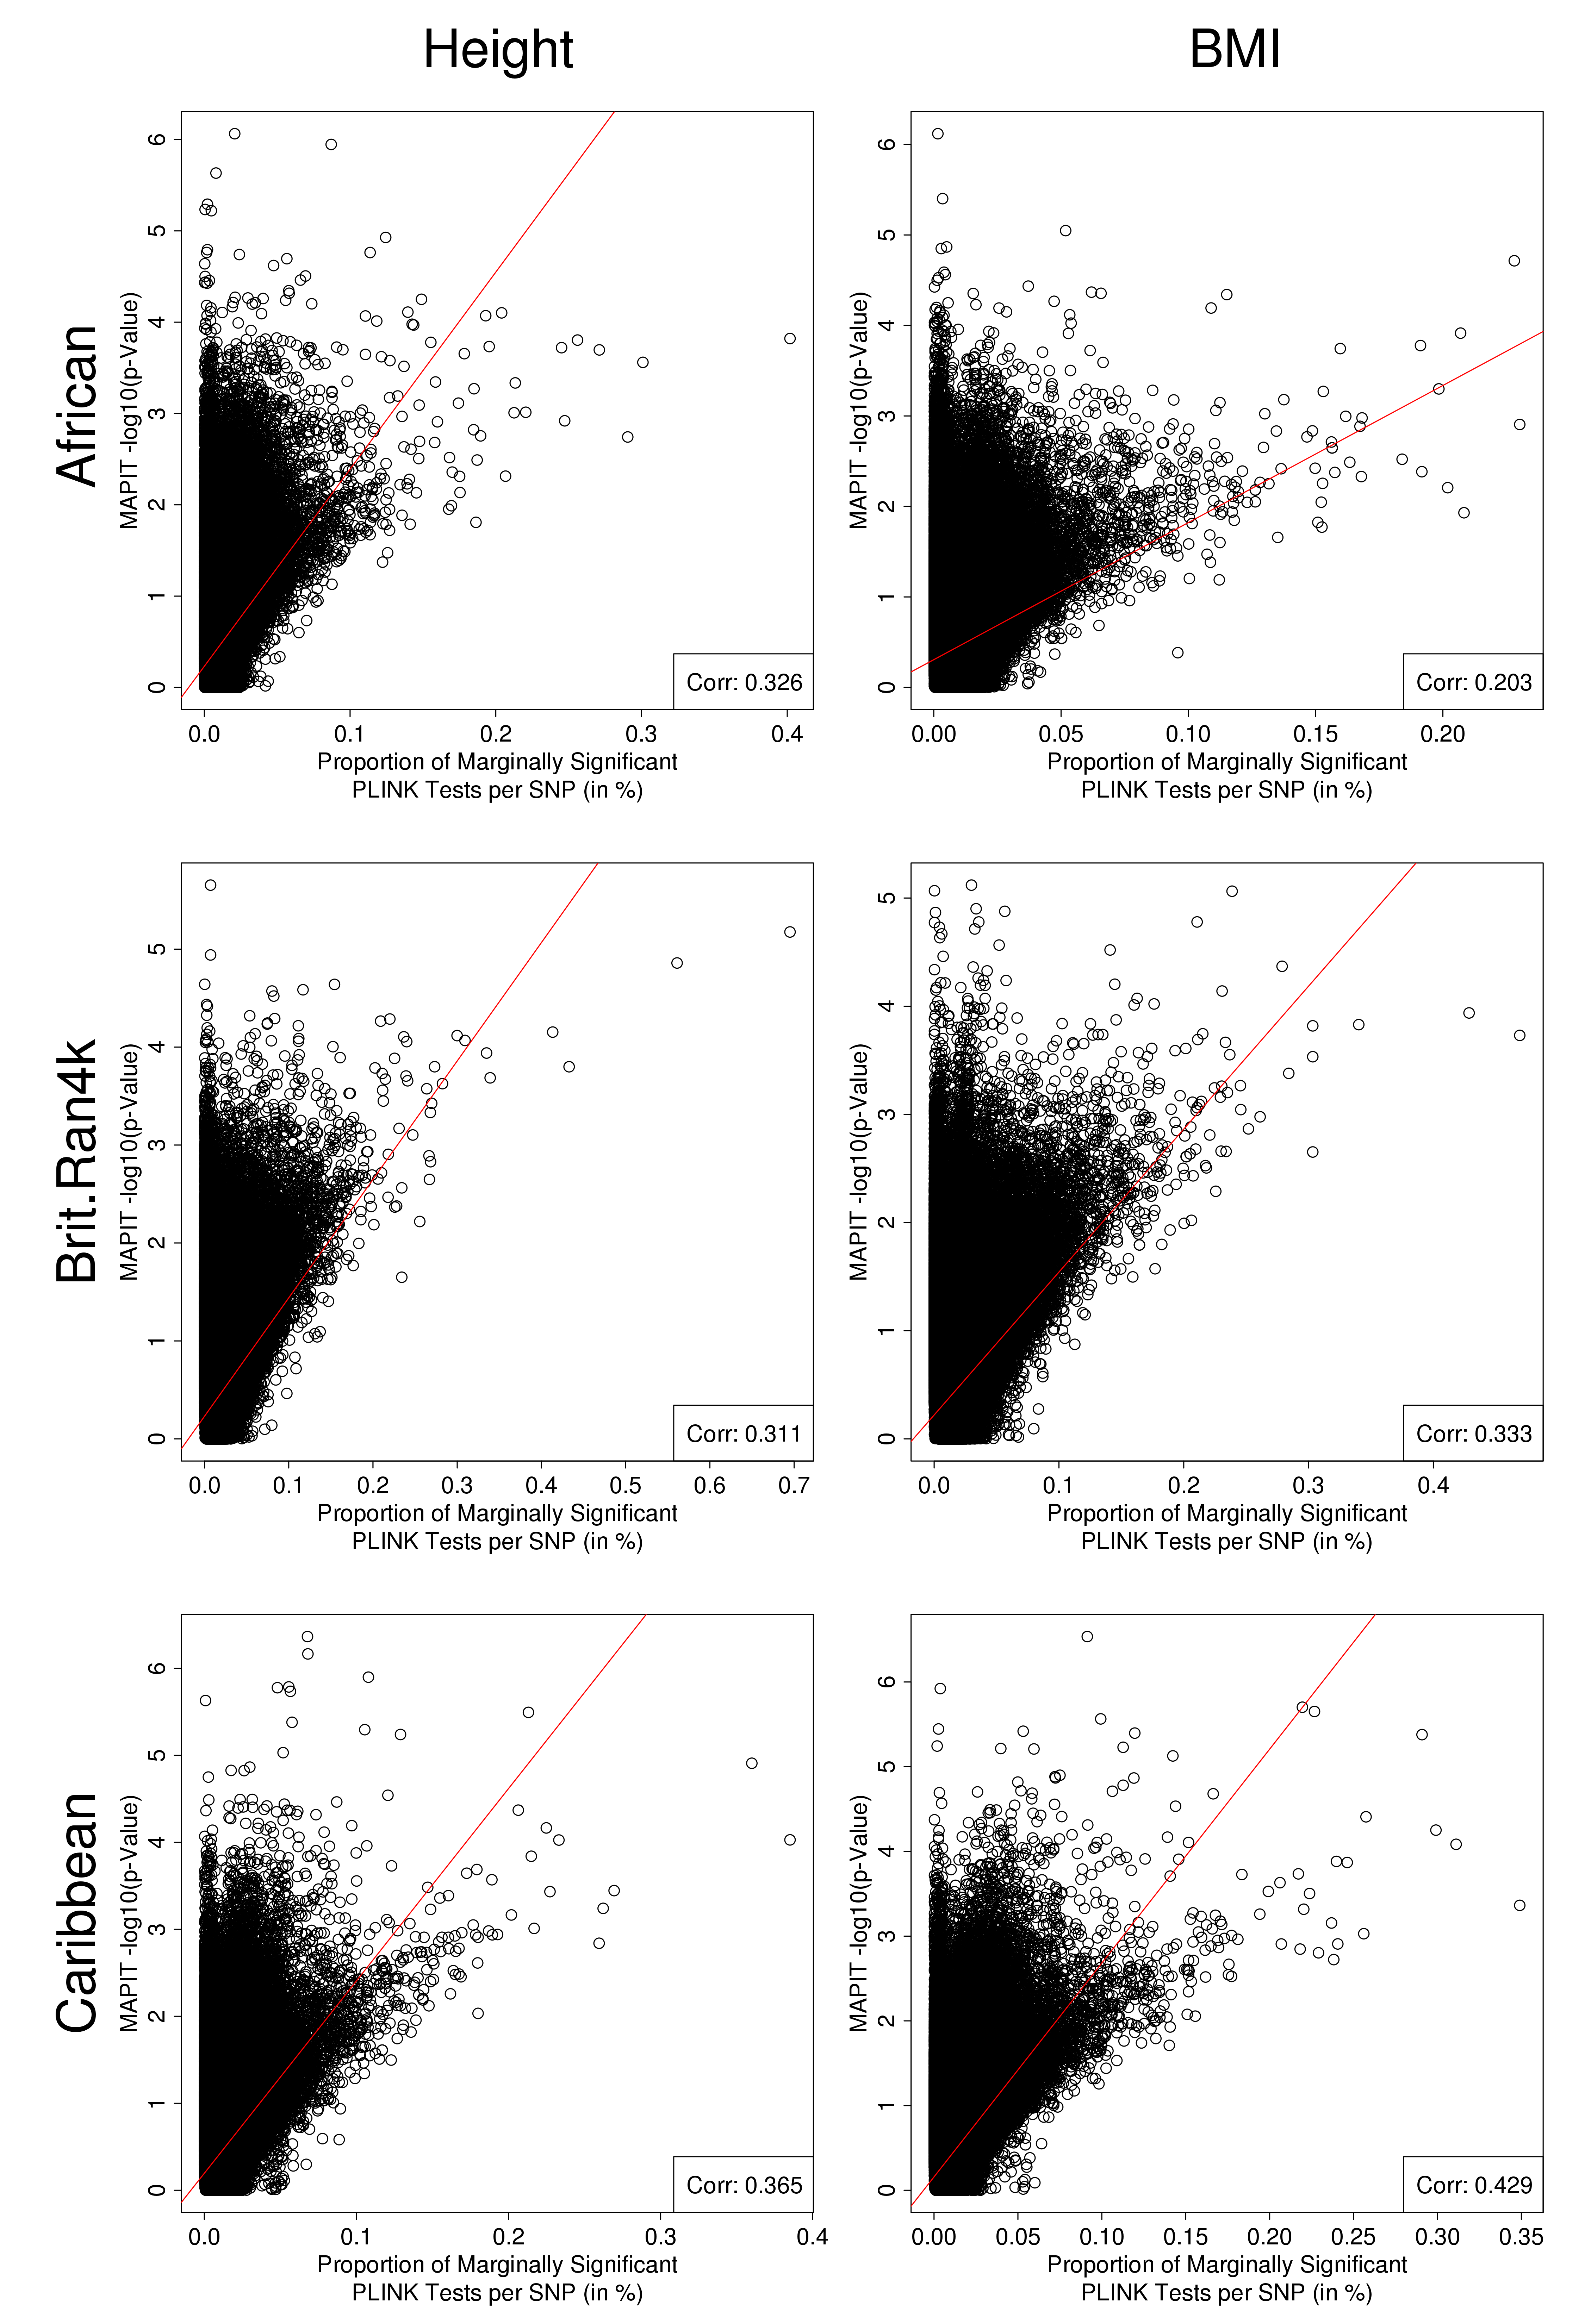
\includegraphics[scale=.3]{Images/Supp/InterPath_Supp_Figure_PLINKvsMAPIT_vs3_AllPops_HeightBMI_pt1.png}
\caption[TBD]{\textbf{Comparison of single-SNP epistasis methods in height and BMI, per subset}. Caption continued at end of figures.}
\label{InterPath-Supp-Figure-MAPITvsPLINK-HeightBMI-AllPops-a}
\end{figure}
\clearpage
\setlength{\footskip}{1cm}
\addtocounter{figure}{-1}

\setlength{\footskip}{3cm}
\begin{figure}[htbp]
\centering
\vspace*{-2cm}
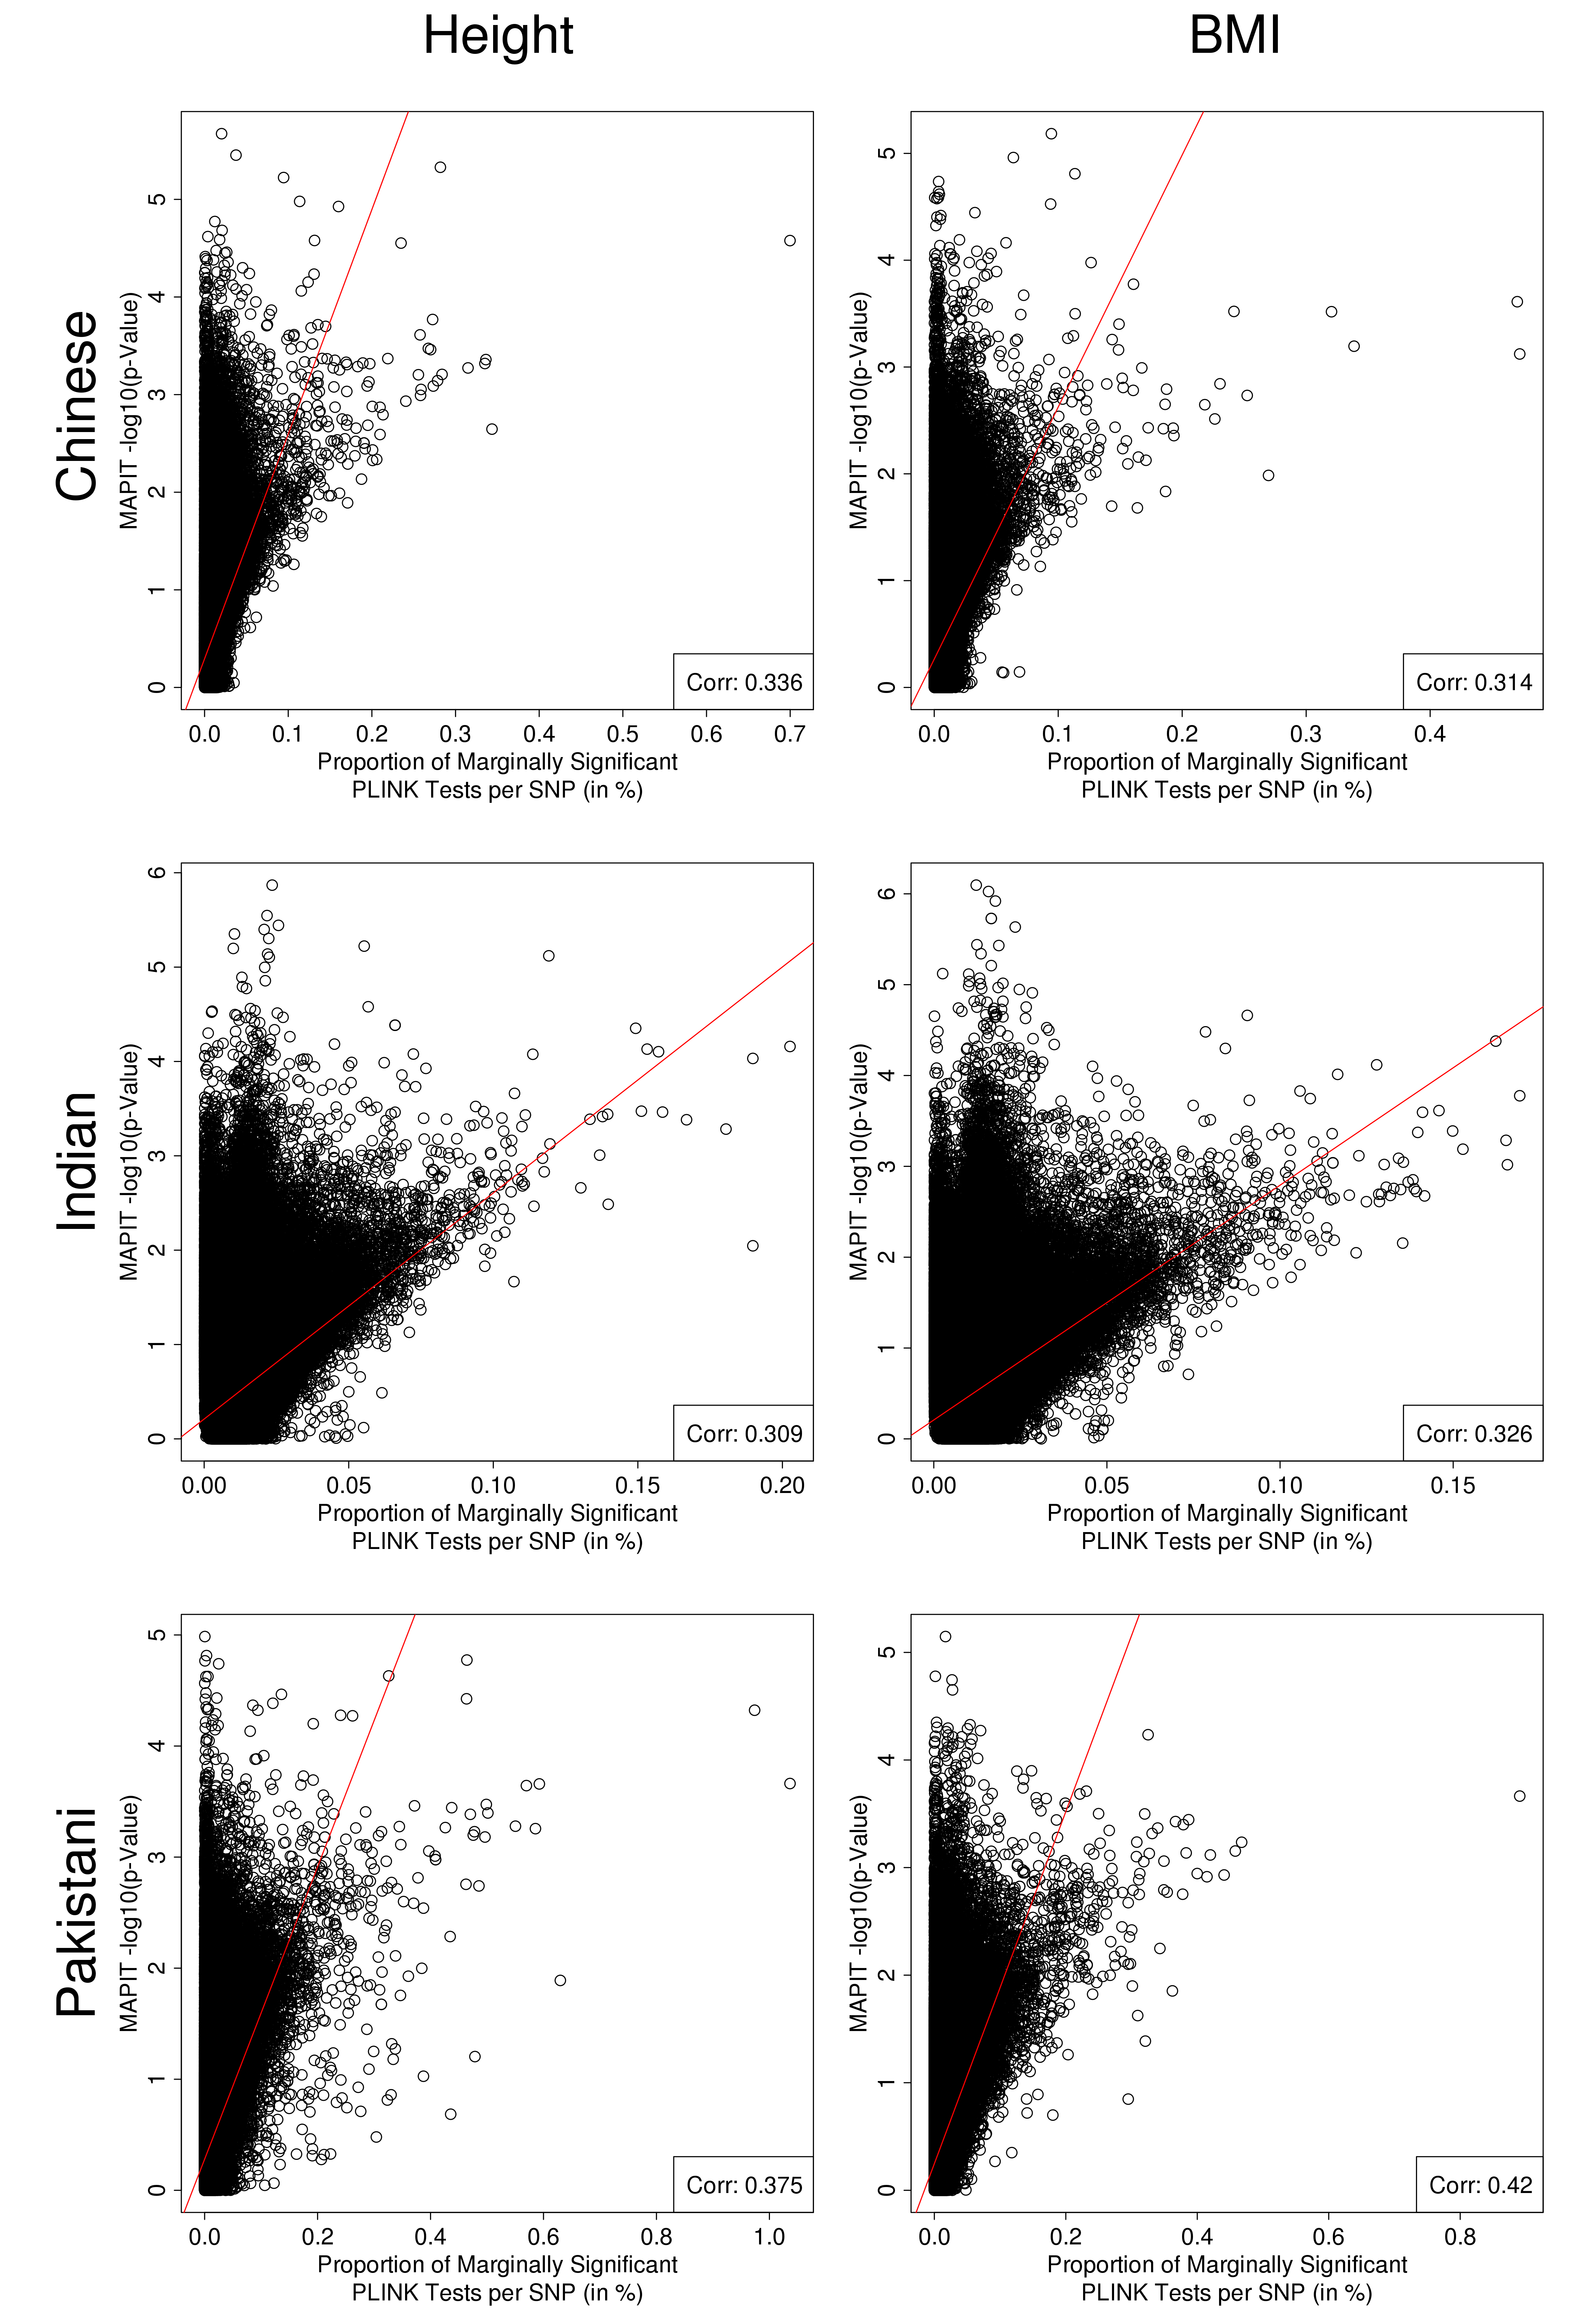
\includegraphics[scale=.3]{Images/Supp/InterPath_Supp_Figure_PLINKvsMAPIT_vs3_AllPops_HeightBMI_pt2.png}
\caption[TBD]{\textbf{Comparison of single-SNP epistasis methods in height and BMI, per subset}. Caption continued at end of figure.}
\label{InterPath-Supp-Figure-MAPITvsPLINK-HeightBMI-AllPops-b}
\end{figure}
\clearpage
\setlength{\footskip}{1cm}
\addtocounter{figure}{-1}

\begin{figure} [t!]
\caption[TBD]{\textbf{Comparison of single-SNP epistasis methods in height and BMI, per subset}. The figure shows the single-SNP PLINK results vs. MAPIT results for height and BMI in each UKB subset. For each individual plot, the PLINK results are shown on the $x$-axis as the proportion of marginally significant interactions per SNP (where marginally significant is defined as $p$-value $<= 1\times10^{-4}$) and the MAPIT results are shown on the $y$-axis as the -$\log_{10}$ of the MAPIT $p$-values. The dotted red line shows the line of best fit, and the correlation between the two metrics is shown in the legend. For many of these plots we observe a subset of SNPs with greater marginal epistasis (higher -$\log_{10}$ $p$-values) beginning to correlate with having larger proportions of marginally significant SNP-by-SNP interactions. Seeing the same signal between two different approaches suggests there may be evidence for epistasis on the single-SNP level, albeit weak.}
\label{InterPath-Supp-Figure-MAPITvsPLINK-HeightBMI-All-caption}
\end{figure}
\clearpage

\begin{figure}[htbp]
\centering
\hspace*{-.9cm}
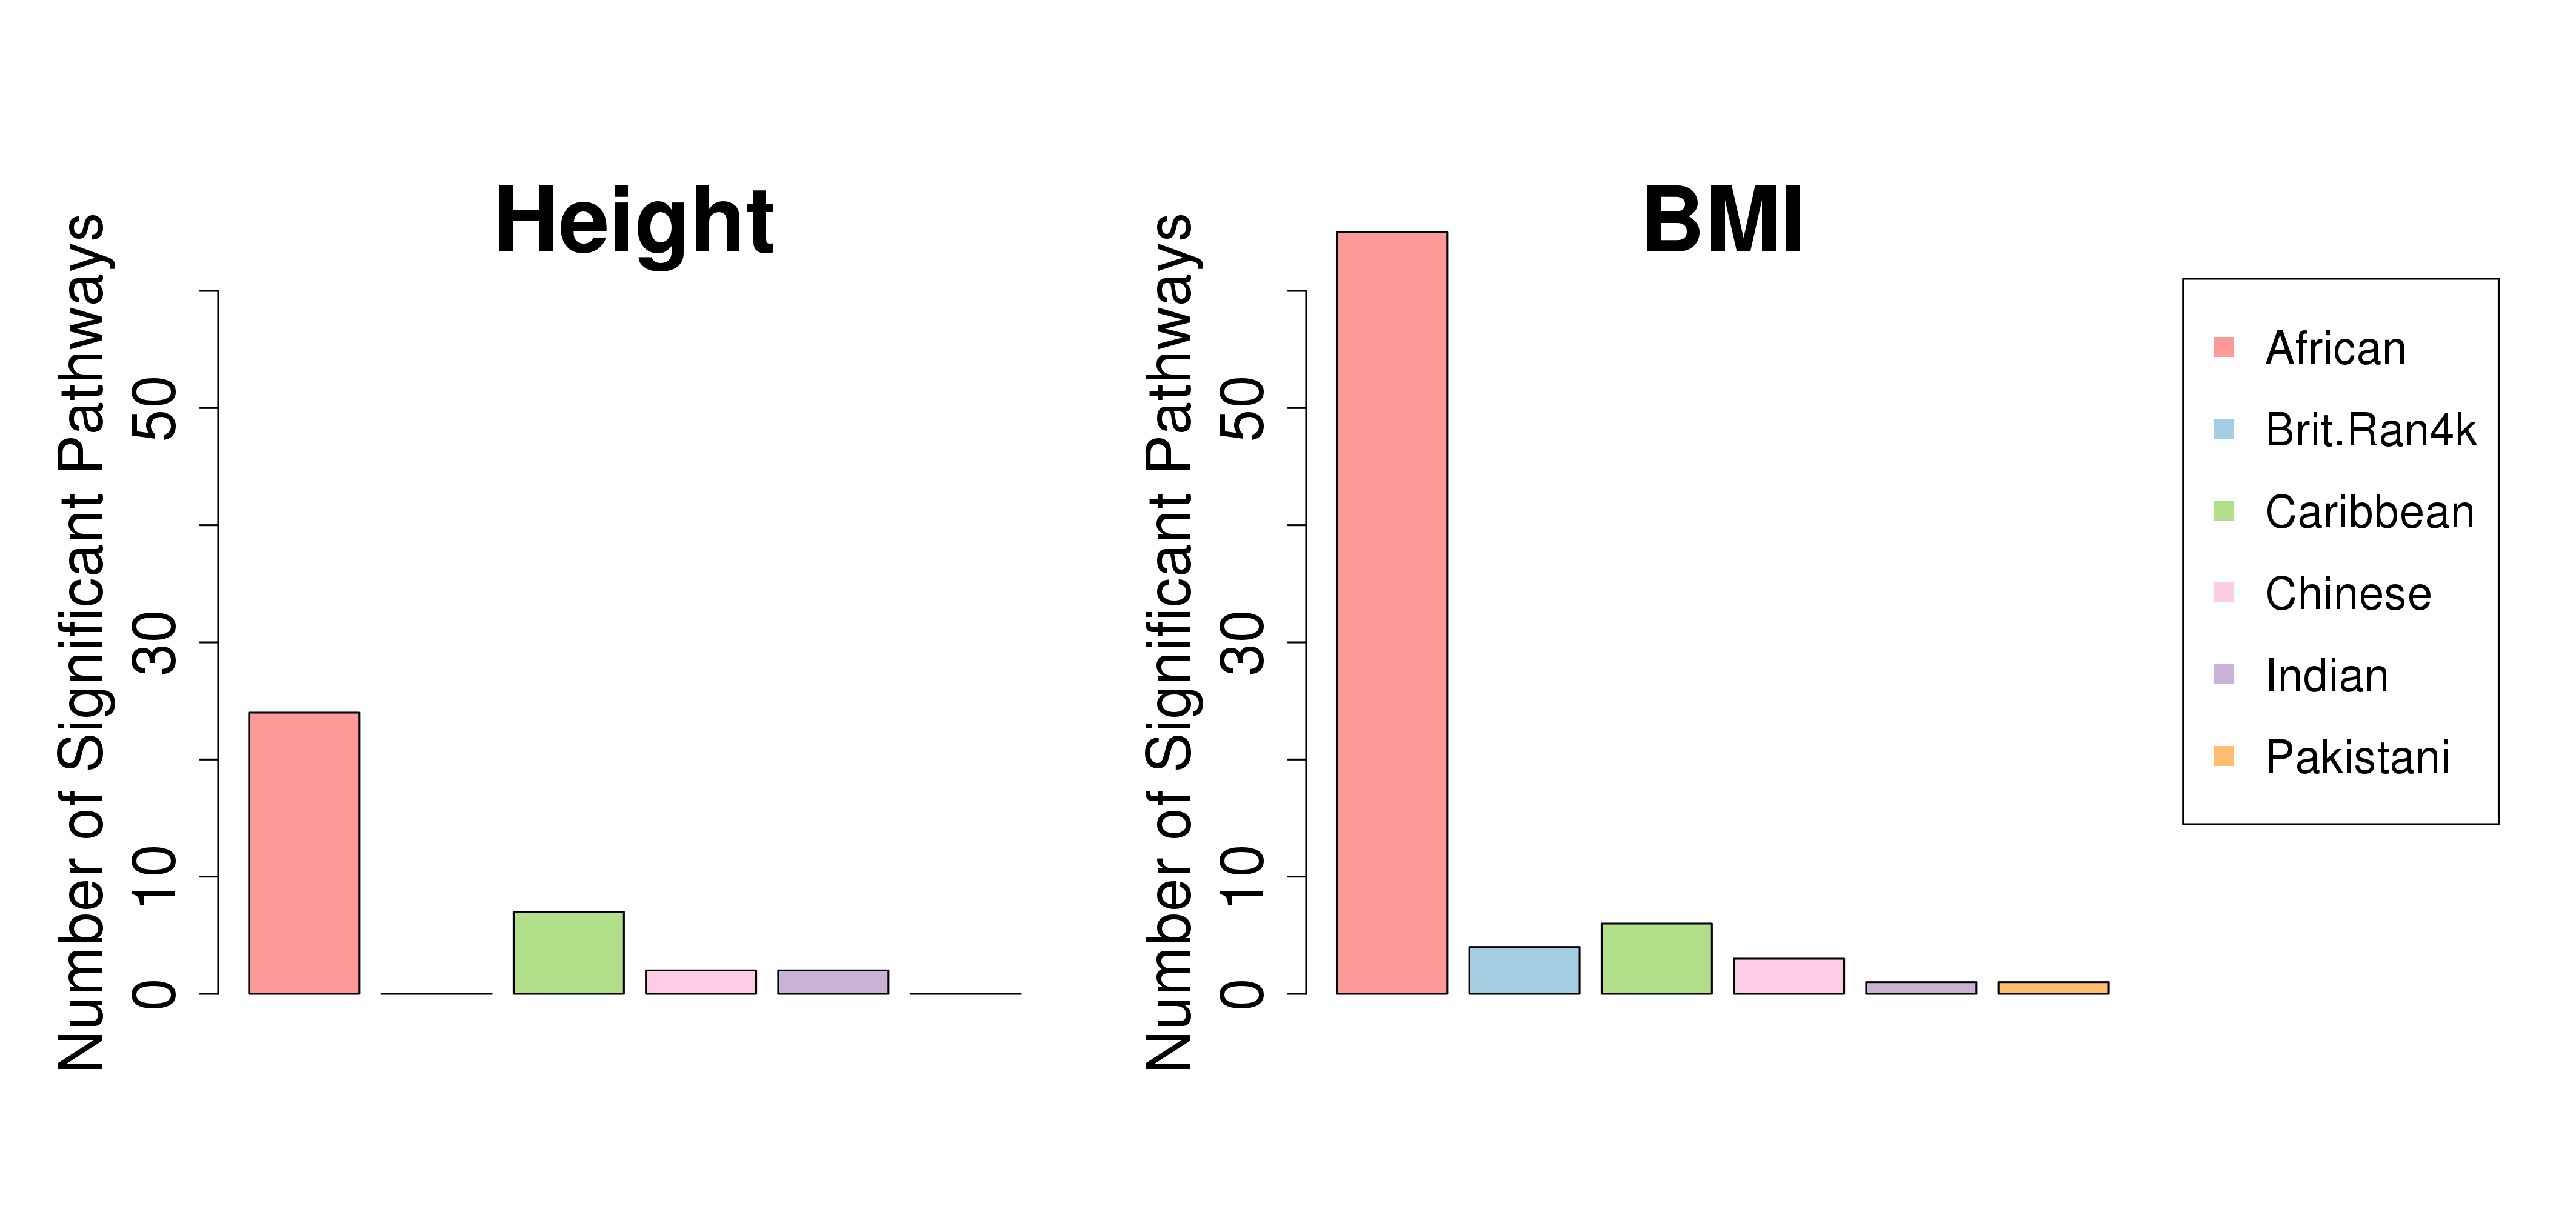
\includegraphics[scale=.45]{Images/Supp/InterPath_Supp_Figure_Barplots_REACTOME_vs2.png}
\caption[TBD]{\textbf{Numbers of REACTOME pathways that have significant marginal epistasis, per subset}. The barplots show the number of genome-wide significant pathways found from running MAPIT-R for both height and BMI in the REACTOME database on each of our UKB subsets. Genome-wide significance was determined by using Bonferroni-corrected $p$-value thresholds based on the number of pathways tested in each phenotype, subset, and pathway database combination. As shown in these results, we find across all phenotype and database combinations that the African subset has the largest numbers of significant pathways. For lists of the specific significant pathways per subset, phenotype, and database combination, see Supplementary Tables \ref{InterPath-Supp-Table-TopPathways-KEGG-Height-a}\textcolor{blue}{-d}.}
\label{InterPath-Supp-Figure-Barplots-REACTOME}
\end{figure}
\clearpage

\begin{figure}[htbp]
\centering
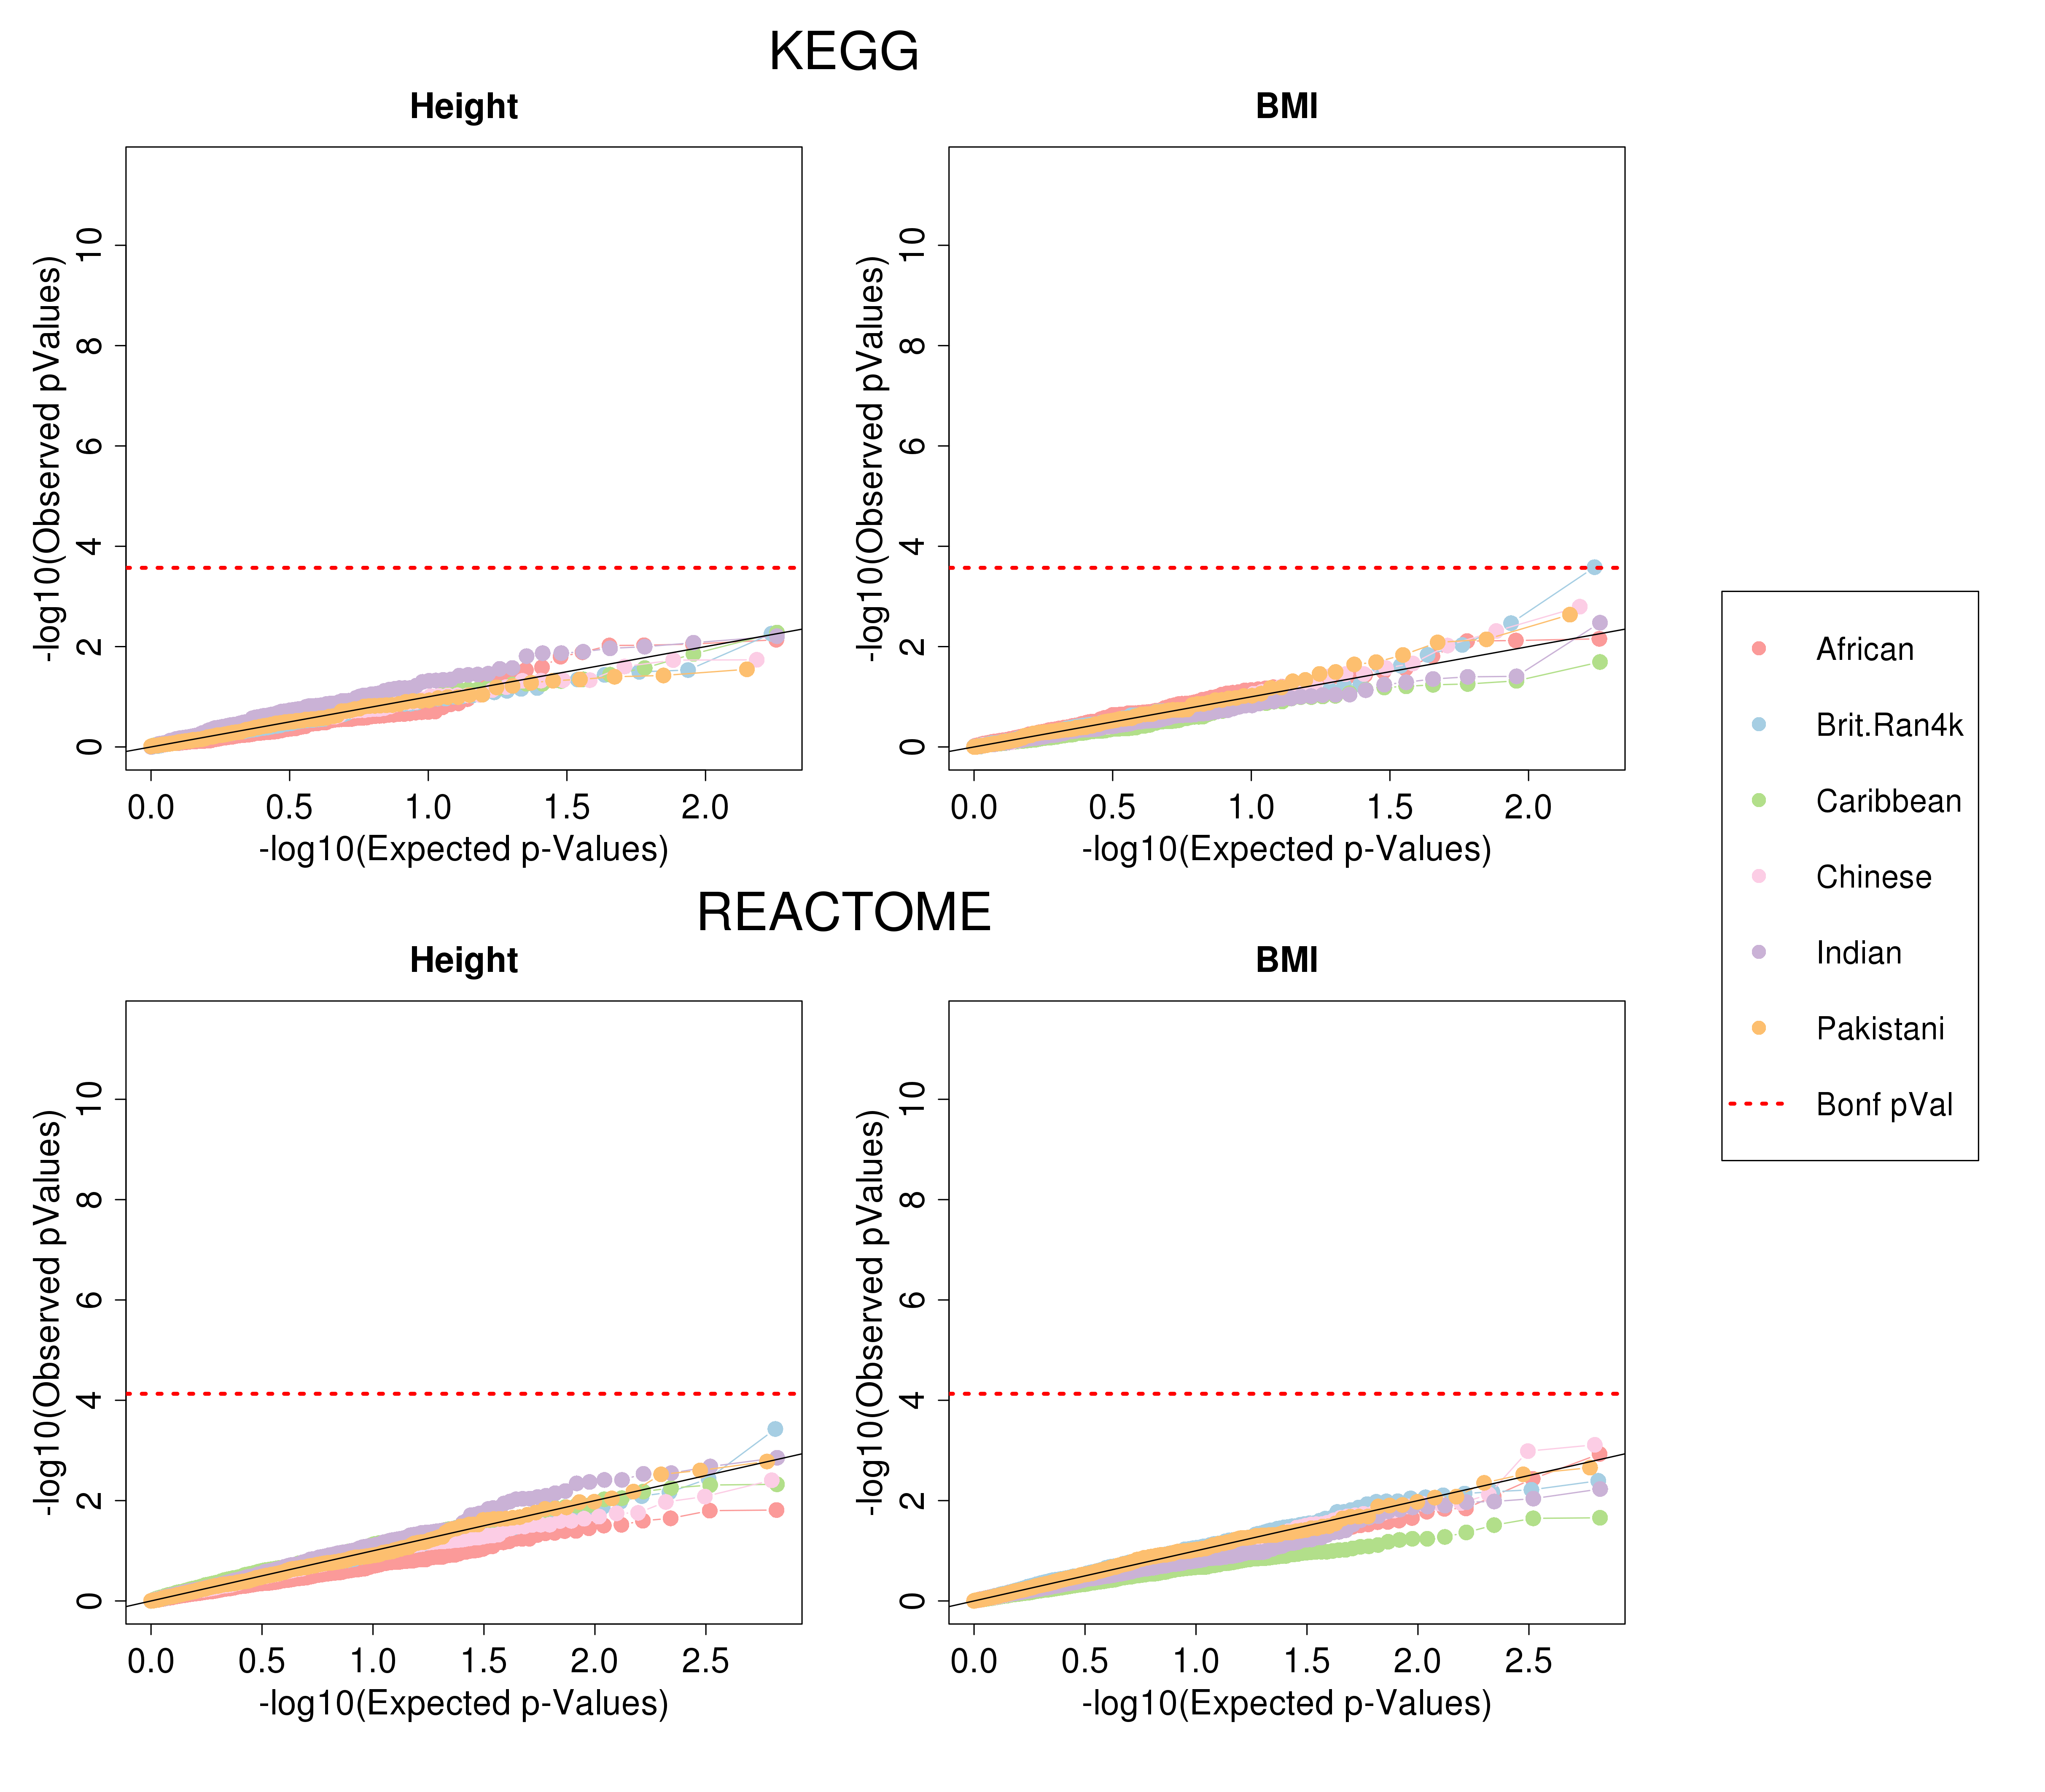
\includegraphics[scale=.35]{Images/Supp/InterPath_Supp_Figure_perm1_QQPlots_AllPaths_vs2.png}
\caption[TBD]{\textbf{QQ-Plots of MAPIT-R results using permuted phenotypes, per subset}. The figure shows QQ-plots for running MAPIT-R using single, permuted versions of both height and BMI with the KEGG \& REACTOME databases. Phenotypes were permuted within each population subset. Shown on the $x$-axis are the -$\log_{10}$ of the expected $p$-values and the on the $y$-axis are on the -$\log_{10}$ of the observed $p$-values. The dotted red line is our Bonferroni-corrected $p$-value threshold based on the number of pathways tested per phenotype and pathway database combination. We find across all UKB subset, phenotype, and pathway database combinations that MAPIT-R displays null behavior within the range expected when using permuted phenotypes.}
\label{InterPath-Supp-Figure-perm1-QQPlots-AllPaths}
\end{figure}
\clearpage

\setlength{\footskip}{3cm}
\begin{figure}[htbp]
\centering
\vspace*{-2cm}
\includegraphics[scale=.2]{Images/Supp/InterPath_Supp_Figure_pValHists_vs3.png}
\caption[TBD]{\textbf{$p$-Value histograms of MAPIT-R results using permuted phenotypes, per subset}. The figure shows histograms of MAPIT-R $p$-values collected across ten independent phenotype permutation runs for each UKB subset. The same phenotype permutation for a given subset was used across both pathway databases (i.e. 10 permutations were done for height and 10 done for BMI for each subset). Covariates used from the original MAPIT-R analysis were kept the same.}
\label{InterPath-Supp-Figure-10perms-pValHists}
\end{figure}
\clearpage
\setlength{\footskip}{1cm}

\setlength{\footskip}{3cm}
\begin{figure}[htbp]
\centering
\vspace*{-2cm}
\includegraphics[scale=.2]{Images/Supp/InterPath_Supp_Figure_pValsVsNumSNPs_vs2.png}
\caption[TBD]{\textbf{Number of SNPs in a pathway versus a pathway's MAPIT-R $p$-value}. Caption continued on next page.}
\label{InterPath-Supp-Figure-pValsVsNumSNPs}
\end{figure}
\clearpage
\setlength{\footskip}{1cm}

\addtocounter{figure}{-1}
\begin{figure} [t!]
  \caption{\textbf{Number of SNPs in a pathway versus a pathway's MAPIT-R $p$-value}. The figure shows plots comparing the MAPIT-R $p$-values from our main analysis to the number of SNPs present in each pathway. Results for every UKB subset, phenotype, and pathway database combinations are shown. The dotted red line is the line of best fit and the legend provides the regression coefficient and its associated $p$-value. We observe that for most combinations there is a significant relationship between MAPIT-R $p$-value and the number of SNPs present in a pathway. This follows our hypothesis that combining SNPs together in a joint analysis might provide greater power to detect marginal epistasis than analyzing each SNP independently. We note, however, that these results appear to not solely be driven just by the presence or absence of large SNP counts -- conducting this same analysis on one of our sets of permuted phenotypes we now find very few significant relationships between MAPIT-R $p$-values and pathway SNP counts (Supplementary Figure \ref{InterPath-Supp-Figure-pValsVsNumSNPs-perm1}).}
\label{InterPath-Supp-Figure-pValsVsNumSNPs-Caption}
\end{figure}
\clearpage

\setlength{\footskip}{3cm}
\begin{figure}[htbp]
\centering
\vspace*{-2cm}
\includegraphics[scale=.2]{Images/Supp/InterPath_Supp_Figure_pValsVsNumSNPs_perm1_vs2.png}
\caption[TBD]{\textbf{Number of SNPs in a pathway versus a pathway's MAPIT-R $p$-value using permuted phenotypes}. Caption continued on next page.}
\label{InterPath-Supp-Figure-pValsVsNumSNPs-perm1}
\end{figure}
\clearpage
\setlength{\footskip}{1cm}

\addtocounter{figure}{-1}
\begin{figure} [t!]
  \caption{\textbf{Number of SNPs in a pathway versus a pathway's MAPIT-R $p$-value using permuted phenotypes}. The figure shows plots comparing the MAPIT-R $p$-values from our main analysis to the number of SNPs present in each pathway. For this analysis a single set of our permuted phenotypes (i.e. Supplementary Figure \ref{InterPath-Supp-Figure-perm1-QQPlots-AllPaths}) was used for each UKB subset. Results for every subset, permuted phenotype, and pathway database combinations are shown. The dotted red line is the line of best fit and the legend provides the regression coefficient and its associated $p$-value. We observe that for very few combinations there is any relationship between MAPIT-R $p$-value and the number of SNPs present in a pathway. For the same analysis on the original set of observed phenotypes, see Supplementary Figure \ref{InterPath-Supp-Figure-pValsVsNumSNPs}.}
\label{InterPath-Supp-Figure-pValsVsNumSNPs-perm1-Caption}
\end{figure}
\clearpage

%\begin{figure}[htbp]
%\centering
%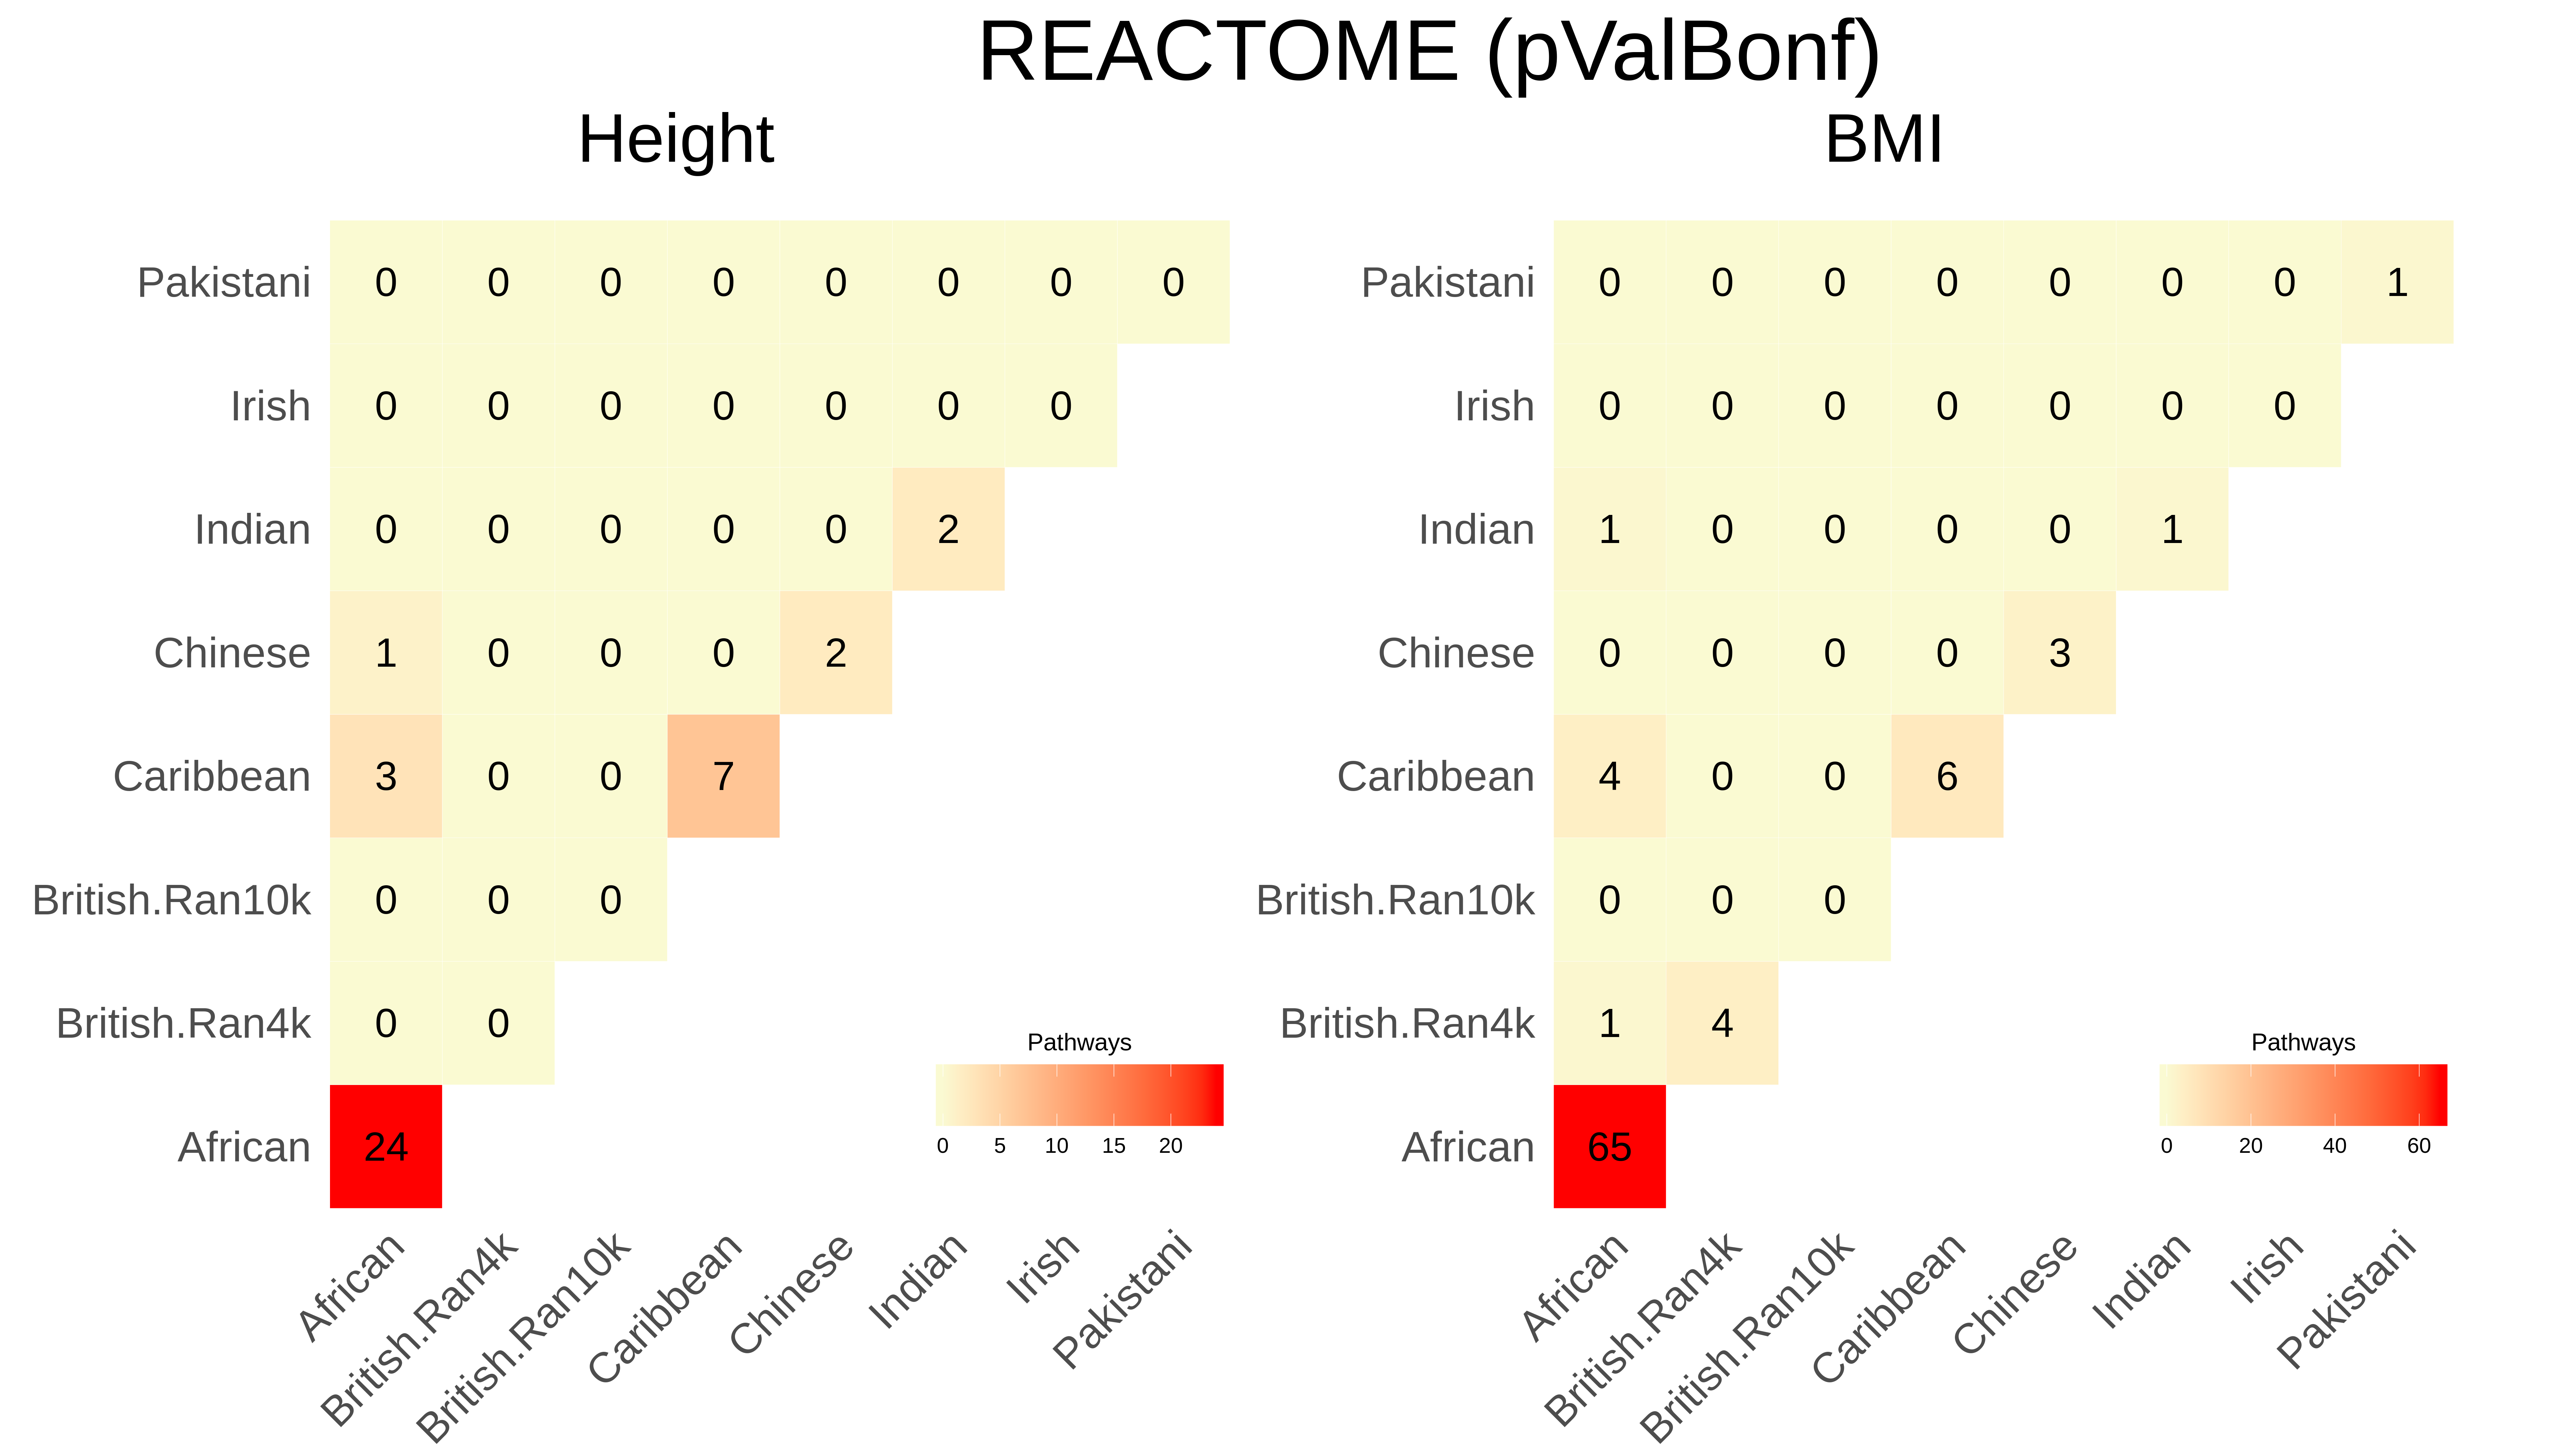
\includegraphics[scale=.225]{Images/Supp/InterPath_Supp_Figure_Heatplots_REACTOME_vs1.png}
%\caption[TBD]{\textbf{TBD}. \\ See above (this would be a supplementary figure).}
%\label{InterPath-Supp-Figure-Heatplots-REACTOME}
%\end{figure}
%\clearpage

\setlength{\footskip}{1cm}
\begin{figure}[htbp]
\centering
\vspace*{-2cm}
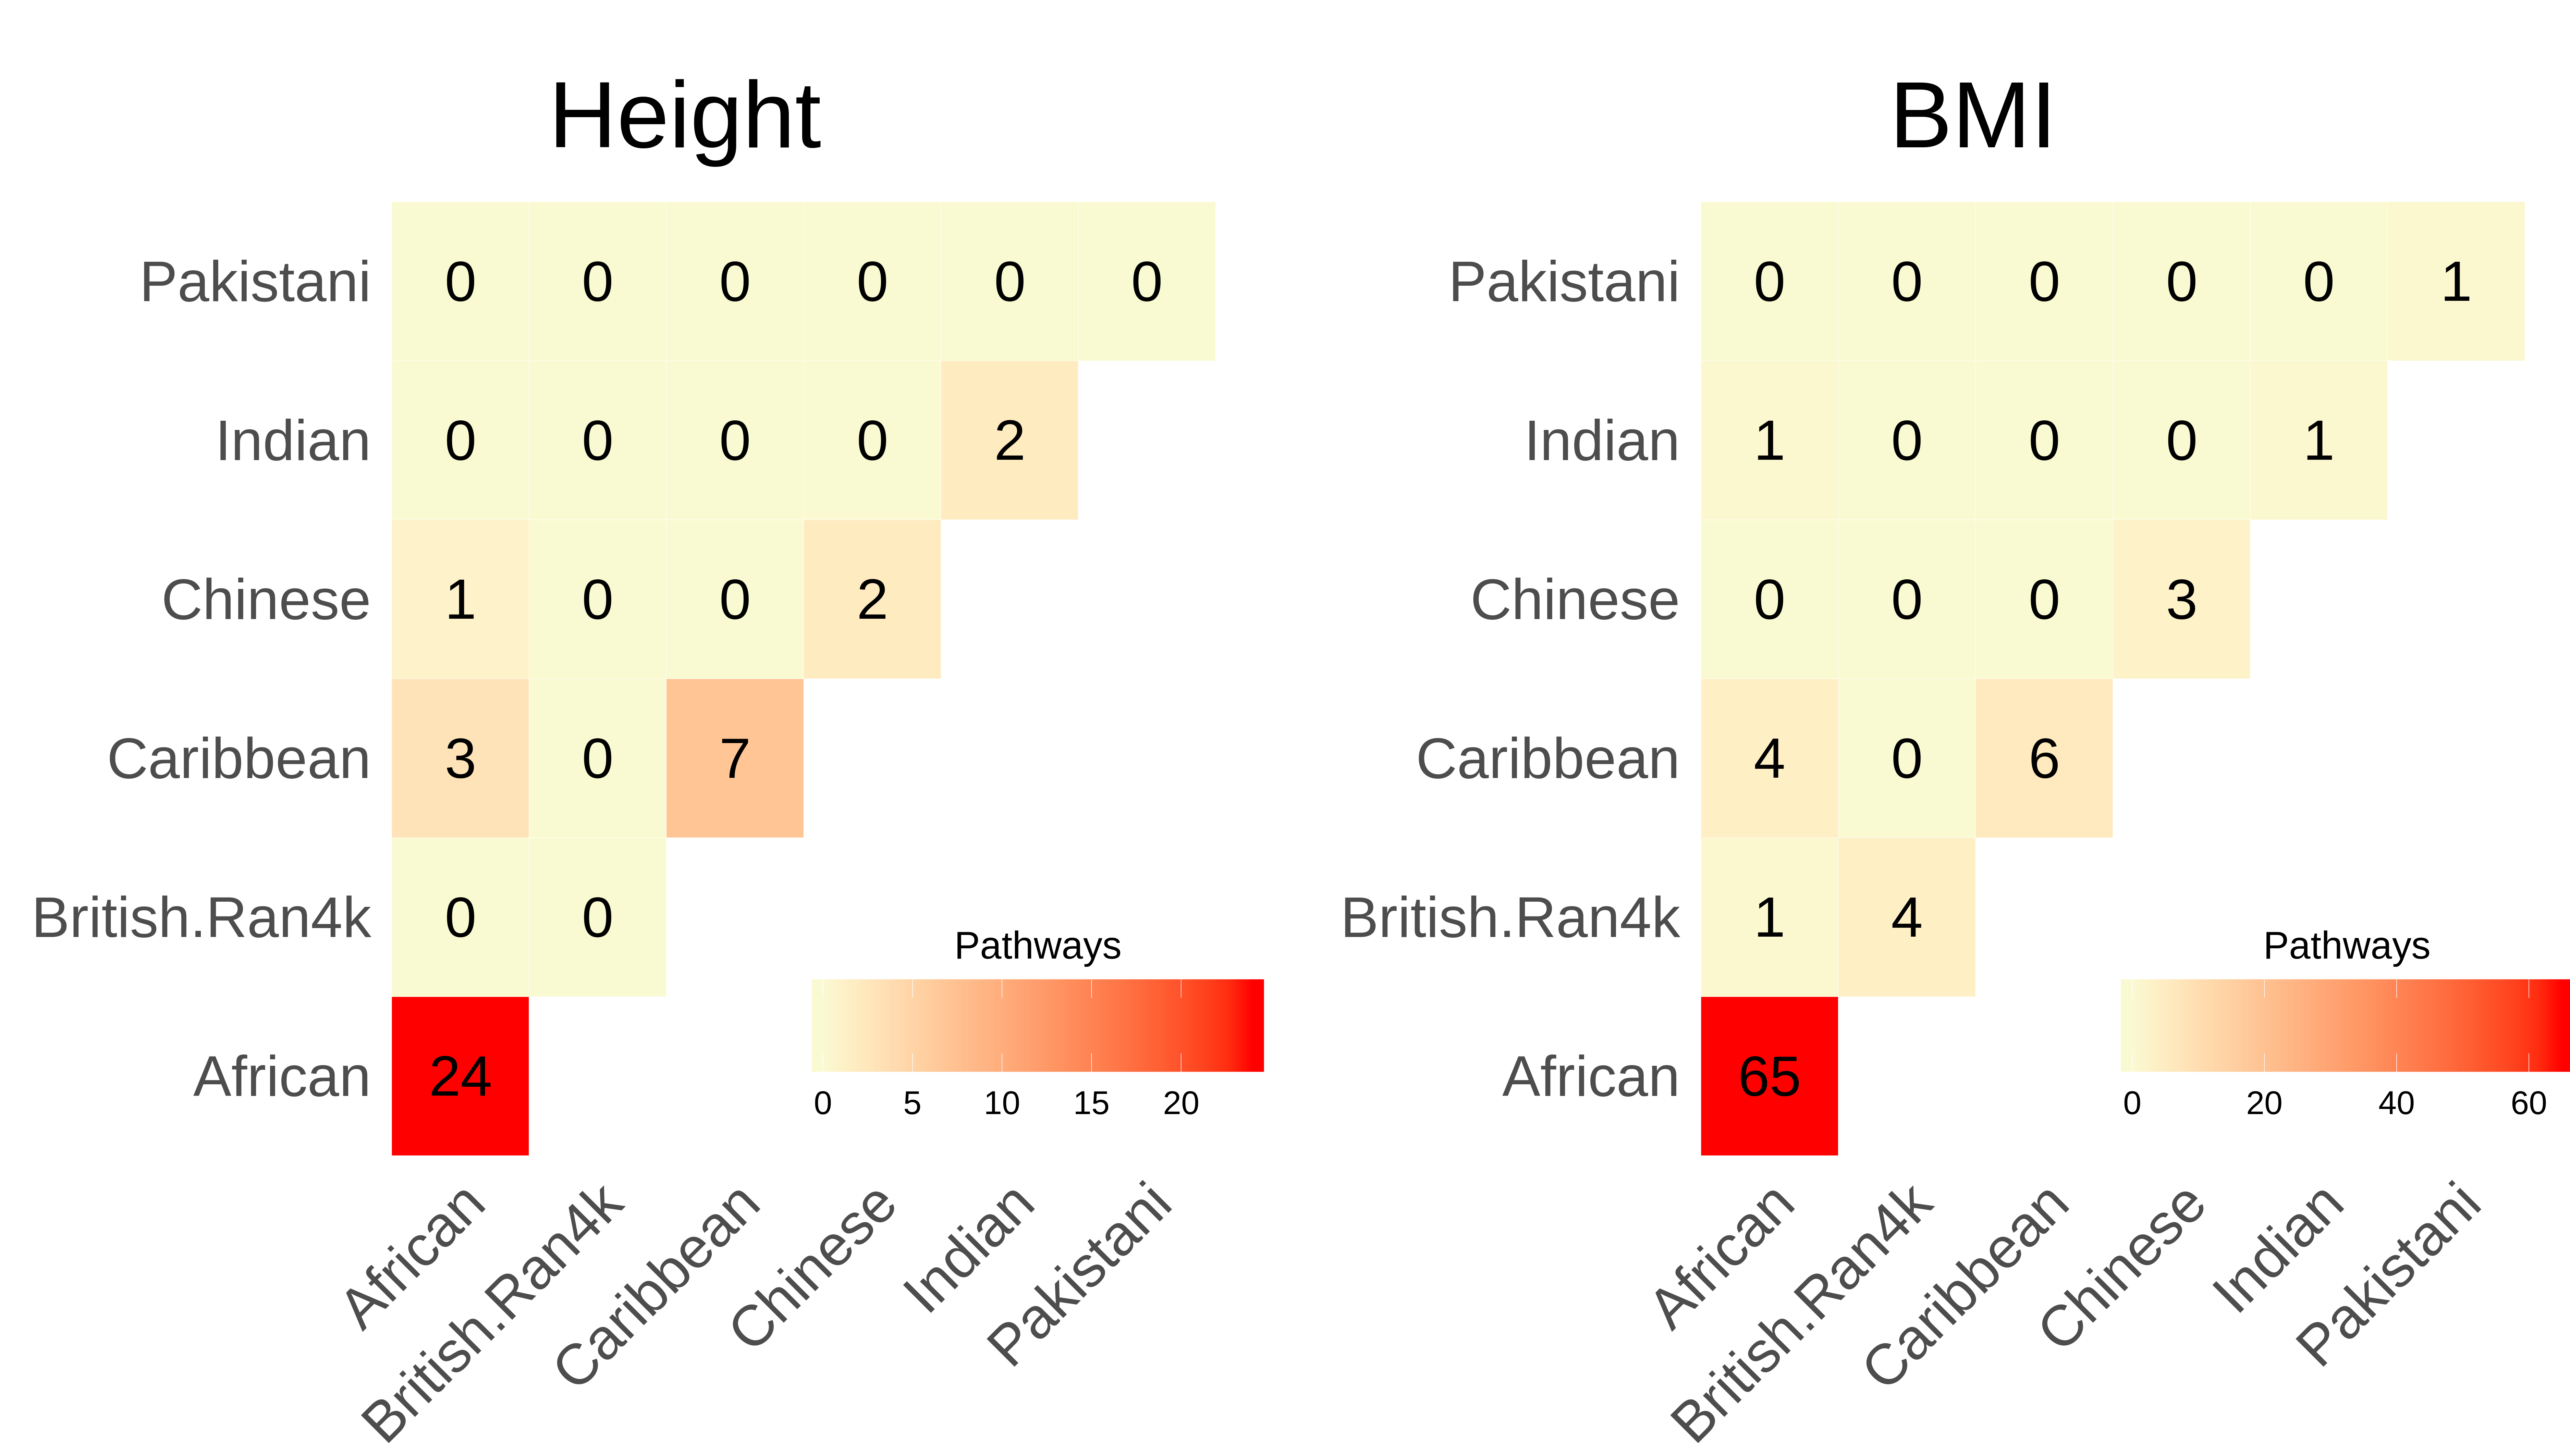
\includegraphics[scale=.225]{Images/Supp/InterPath_Supp_Figure_Heatplots_REACTOME_vs3.png}
\caption[TBD]{\textbf{Overlap of genome-wide significant MAPIT-R pathways between UKB population subsets: REACTOME}. The heatplots show the numbers of genome-wide significant MAPIT-R pathways that overlap between each UKB subset for height and BMI in the REACTOME database. The diagonal shows the total number of genome-wide significant pathways per population subset. We observe that most subsets often have overlap with the African subset but rarely do so with the remaining non-African subsets. For results from the KEGG database see Figure \ref{InterPath-Main-Figure-Heatplots-KEGG}.}
\label{InterPath-Supp-Figure-Heatplots-REACTOME}
\end{figure}
\clearpage
\setlength{\footskip}{1cm}

%\begin{figure}[htbp]
%\centering
%\includegraphics[scale=.15]{Images/Main/InterPath_Main_PopCompDotPlots_African_vs1.png}
%\caption[]{\textbf{MAPIT-R Cross-Population KEGG $p$-value Comparisons: African}. Shown are comparisons of each population subset's MAPIT-R $p$-value for Height and BMI in KEGG against the African subset's MAPIT-R $p$-values. On the $x$-axis are the African subset's observed -$\log_{10}$ $p$-value and on the $y$-axis is the other population's observed -$\log_{10}$ $p$-value. Dotted red lines represent Bonferroni-corrected $p$-value thresholds for each population/phenotype combination.}
%\label{InterPath-Main-Figure-PopCompDotPlots}
%\end{figure}
%\clearpage

%\begin{figure}[htbp]
%\centering
%\includegraphics[scale=.15]{Images/Supp/InterPath_Supp_Figure_PhenoCompDotPlots_vs1.png}
%\caption[TBD]{\textbf{MAPIT-R Phenotype $p$-value Comparisons}. \\ Shown is a comparison of the MAPIT-R $p$-values for both phenotypes analyzed across all population subsets in the KEGG database. Shown on the $x$-axis is the observed height -$\log_{10}$ MAPIT-R $p$-value and shown on the $y$-axis is the observed BMI -$\log_{10}$ MAPIT-R $p$-value. Dotted red lines represent Bonferroni-corrected $p$-value thresholds for each population/phenotype combination (.05 / number of KEGG pathways analyzed). In general we observe a correlation between MAPIT-R $p$-values between each phenotype. In the African subset, where we have the most observed power, we find pathways that are significant in both phenotypes as well as each phenotype separately. Additionally, we observe, among marginally significant pathways, stronger MAPIT-R signals in BMI than height -- this is in line with previous observations that BMI may contain higher levels of epistasis than height (citations).}
%\label{InterPath-Supp-Figure-PhenoCompDotPlots}
%\end{figure}
%\clearpage

\setlength{\footskip}{3cm}
\begin{figure}[htbp]
\centering
\vspace*{-2cm}
\includegraphics[scale=.2]{Images/Supp/InterPath_Supp_Figure_MAPITR_PhenoComps_AllPops_vs3.png}
\caption[TBD]{\textbf{Comparison of MAPIT-R results between height and BMI, per subset}. The figure shows MAPIT-R height results plotted against MAPIT-R BMI results for all pathways from the KEGG and REACTOME databases in all UKB subsets. The $x$-axes are the MAPIT-R height -$\log_{10}$ $p$-values and the $y$-axes are the MAPIT-R BMI -$\log_{10}$ $p$-values. The dotted red lines are the Bonferroni-corrected $p$-value thresholds for genome-wide significance in each subset, pathway, and phenotype combination. The correlation between the phenotype -$\log_{10}$ $p$-values is shown in the bottom right.}
\label{InterPath-Supp-Figure-MAPITR-PhenoComps-AllPops}
\end{figure}
\clearpage
\setlength{\footskip}{1cm}

\begin{figure}[htbp]
\centering
\hspace*{-1.75cm}
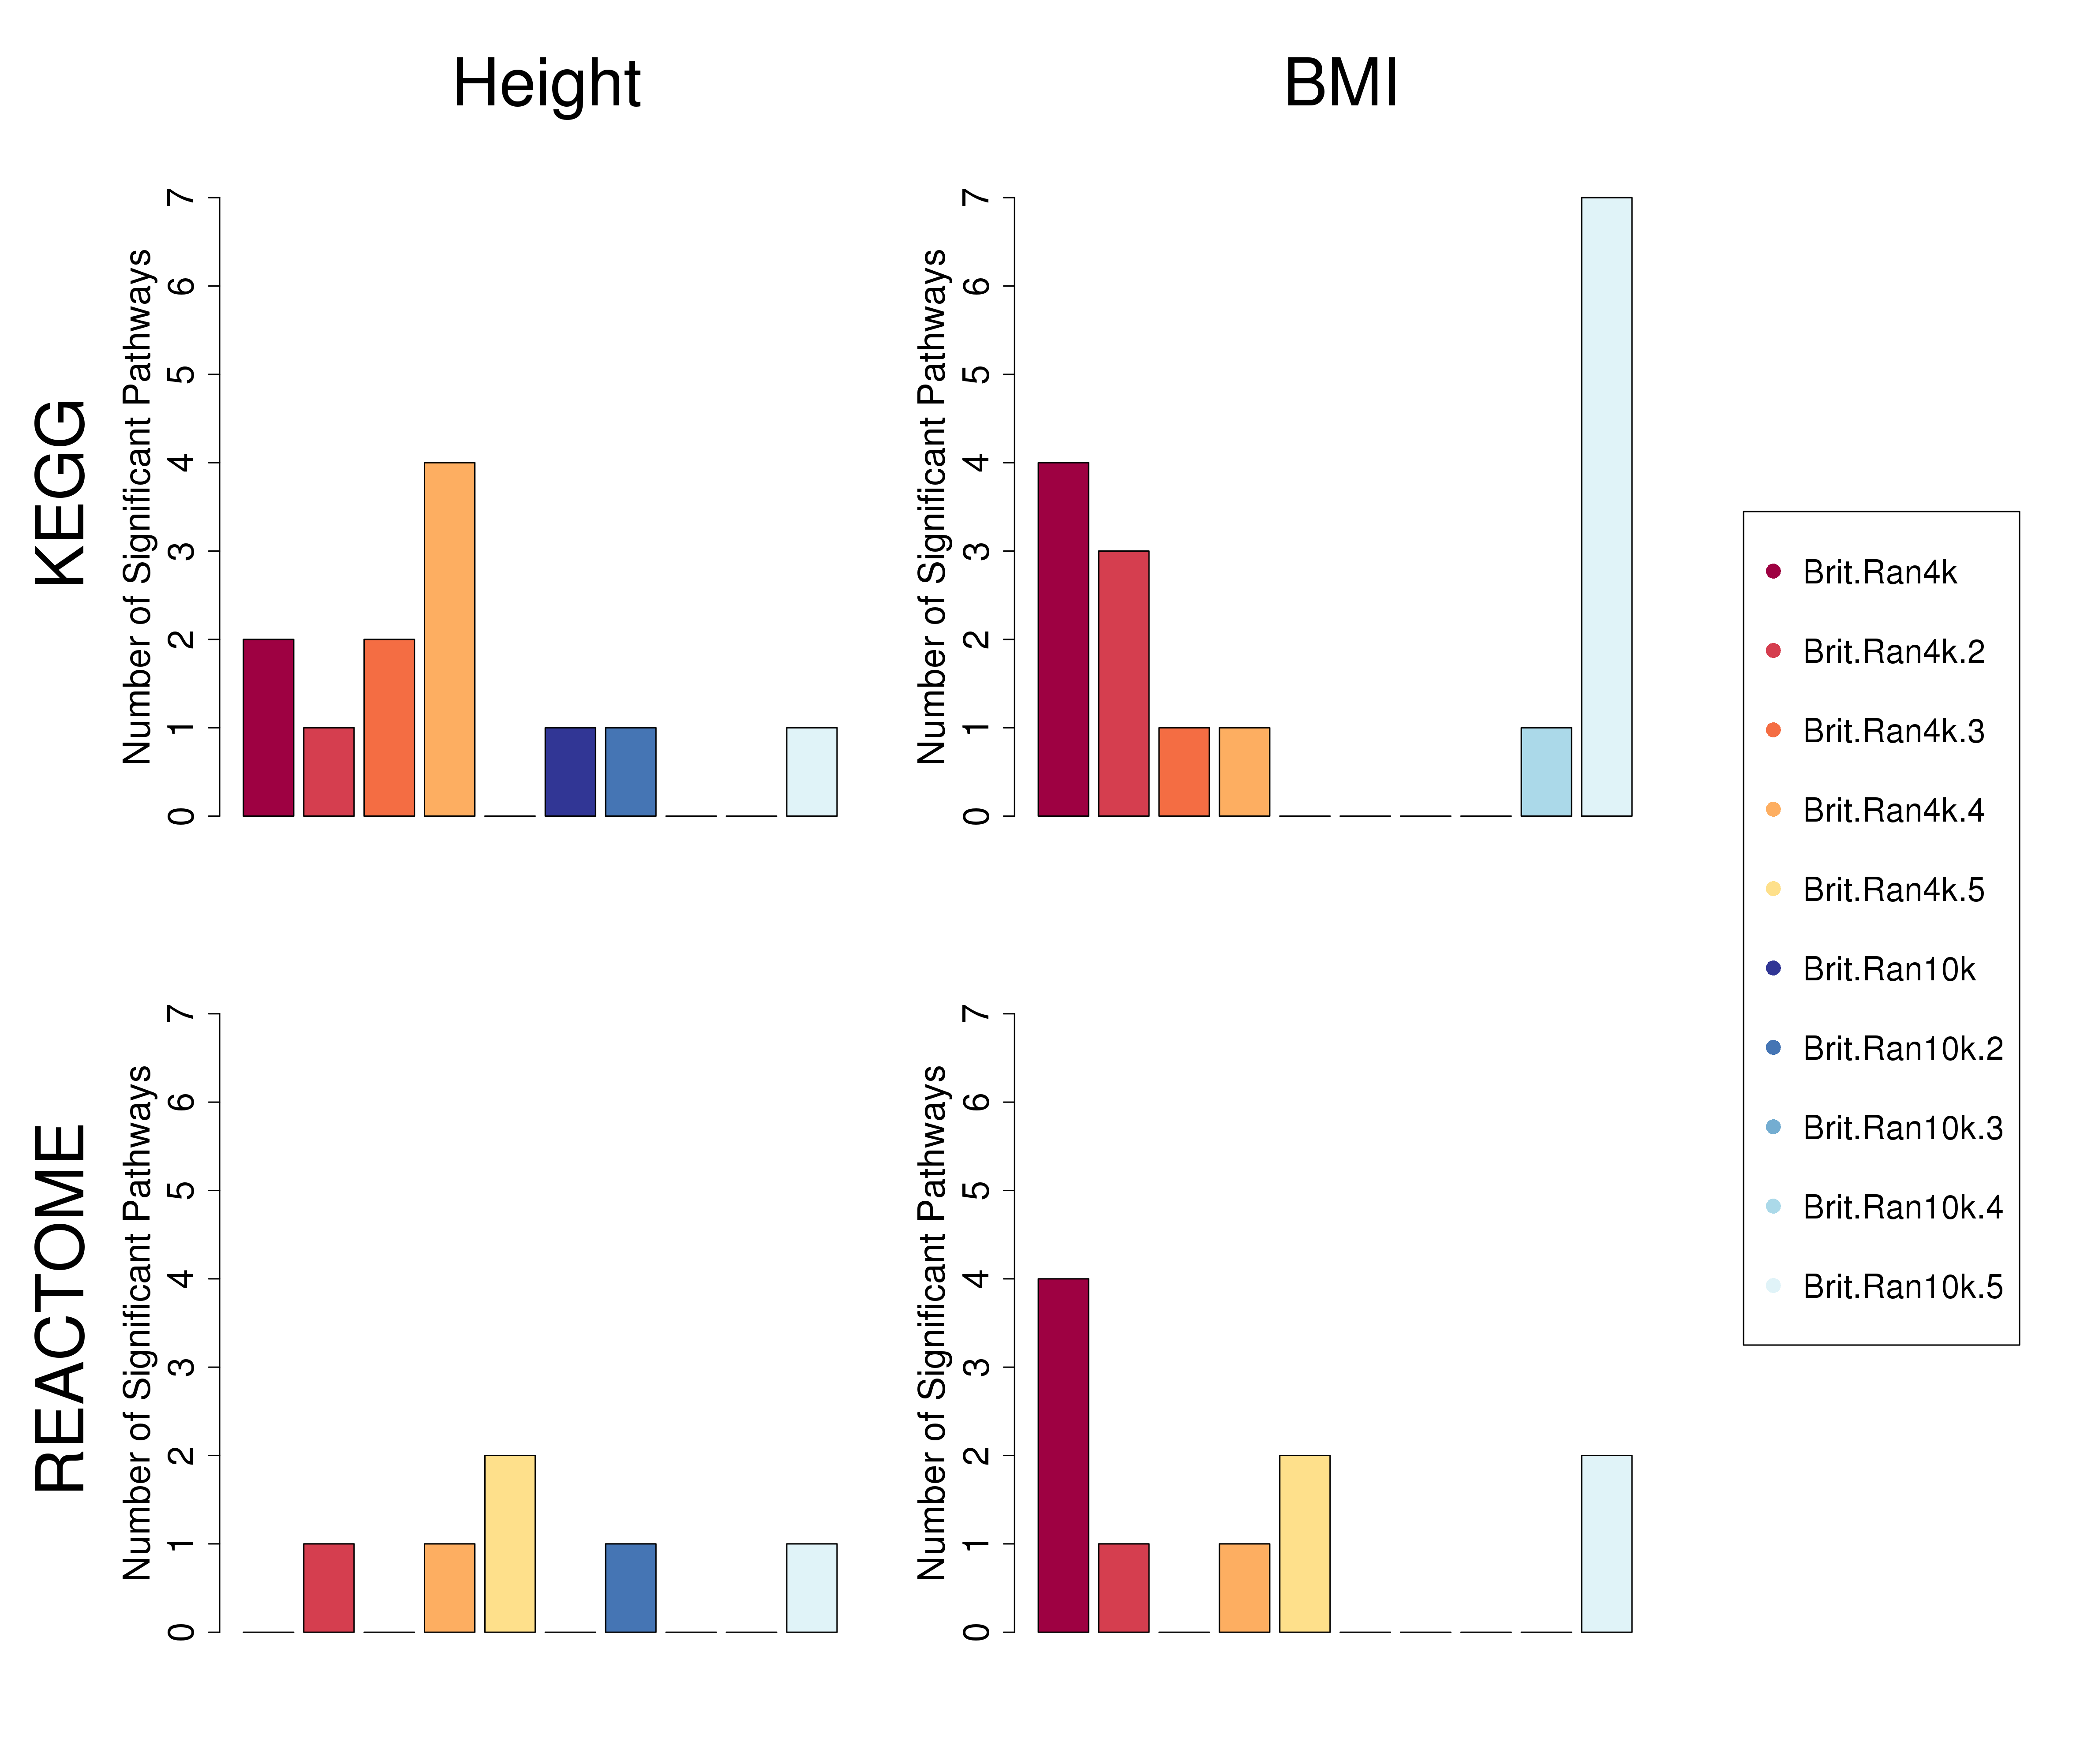
\includegraphics[scale=.45]{Images/Supp/InterPath_Supp_Figure_BritReps_Barplot_vs3.png}
\caption[TBD]{\textbf{Numbers of pathways that have significant marginal epistasis, per British replicate}. The barplots show the number of genome-wide significant pathways found from running MAPIT-R for both height and BMI in the KEGG and REACTOME databases on each of our British subsample replicate populations. Genome-wide significance was determined by using Bonferroni-corrected $p$-value thresholds based on the number of pathways tested in each phenotype, replicate, and pathway database combination. Most replicate runs did not produce many significant results.}
\label{InterPath-Supp-Figure-BritReps-Barplots}
\end{figure}
\clearpage

\newcounter{CharNumber4}
\setcounter{CharNumber4}{1}
\renewcommand{\thefigure}{\arabic{figure}\alph{CharNumber4}}
\begin{landscape}
\begin{figure}[htbp]
\centering
\includegraphics[scale=.2]{Images/Supp/InterPath_Supp_Figure_BritReps_Heatplots_KEGG_vs3.png}
\caption[TBD]{\textbf{Overlap of genome-wide significant MAPIT-R pathways between British replicates subsets: KEGG}. The heatplots show the numbers of genome-wide significant MAPIT-R pathways that overlap between each British replicate subset for height and BMI in the KEGG database. The diagonal shows the total number of genome-wide significant pathways per population subset. We do not observe many genome-wide significant pathways or pathways that overlap between replicate subsets.}
\label{InterPath-Supp-Figure-BritReps-Heatplots-AllPaths-KEGG}
\end{figure}
\clearpage
\addtocounter{figure}{-1}
\addtocounter{CharNumber4}{1}
\end{landscape}

\begin{landscape}
\begin{figure}[htbp]
\centering
\includegraphics[scale=.2]{Images/Supp/InterPath_Supp_Figure_BritReps_Heatplots_REACTOME_vs3.png}
\caption[TBD]{\textbf{Overlap of genome-wide significant MAPIT-R pathways between British replicates subsets: REACTOME}. The heatplots show the numbers of genome-wide significant MAPIT-R pathways that overlap between each British replicate subset for height and BMI in the REACTOME database. The diagonal shows the total number of genome-wide significant pathways per population subset. We do not observe many genome-wide significant pathways or pathways that overlap between replicate subsets.}
\label{InterPath-Supp-Figure-BritReps-Heatplots-AllPaths-REACTOME}
\end{figure}
\clearpage
\end{landscape}
\renewcommand{\thefigure}{\arabic{figure}}

\begin{figure}[htbp]
\centering
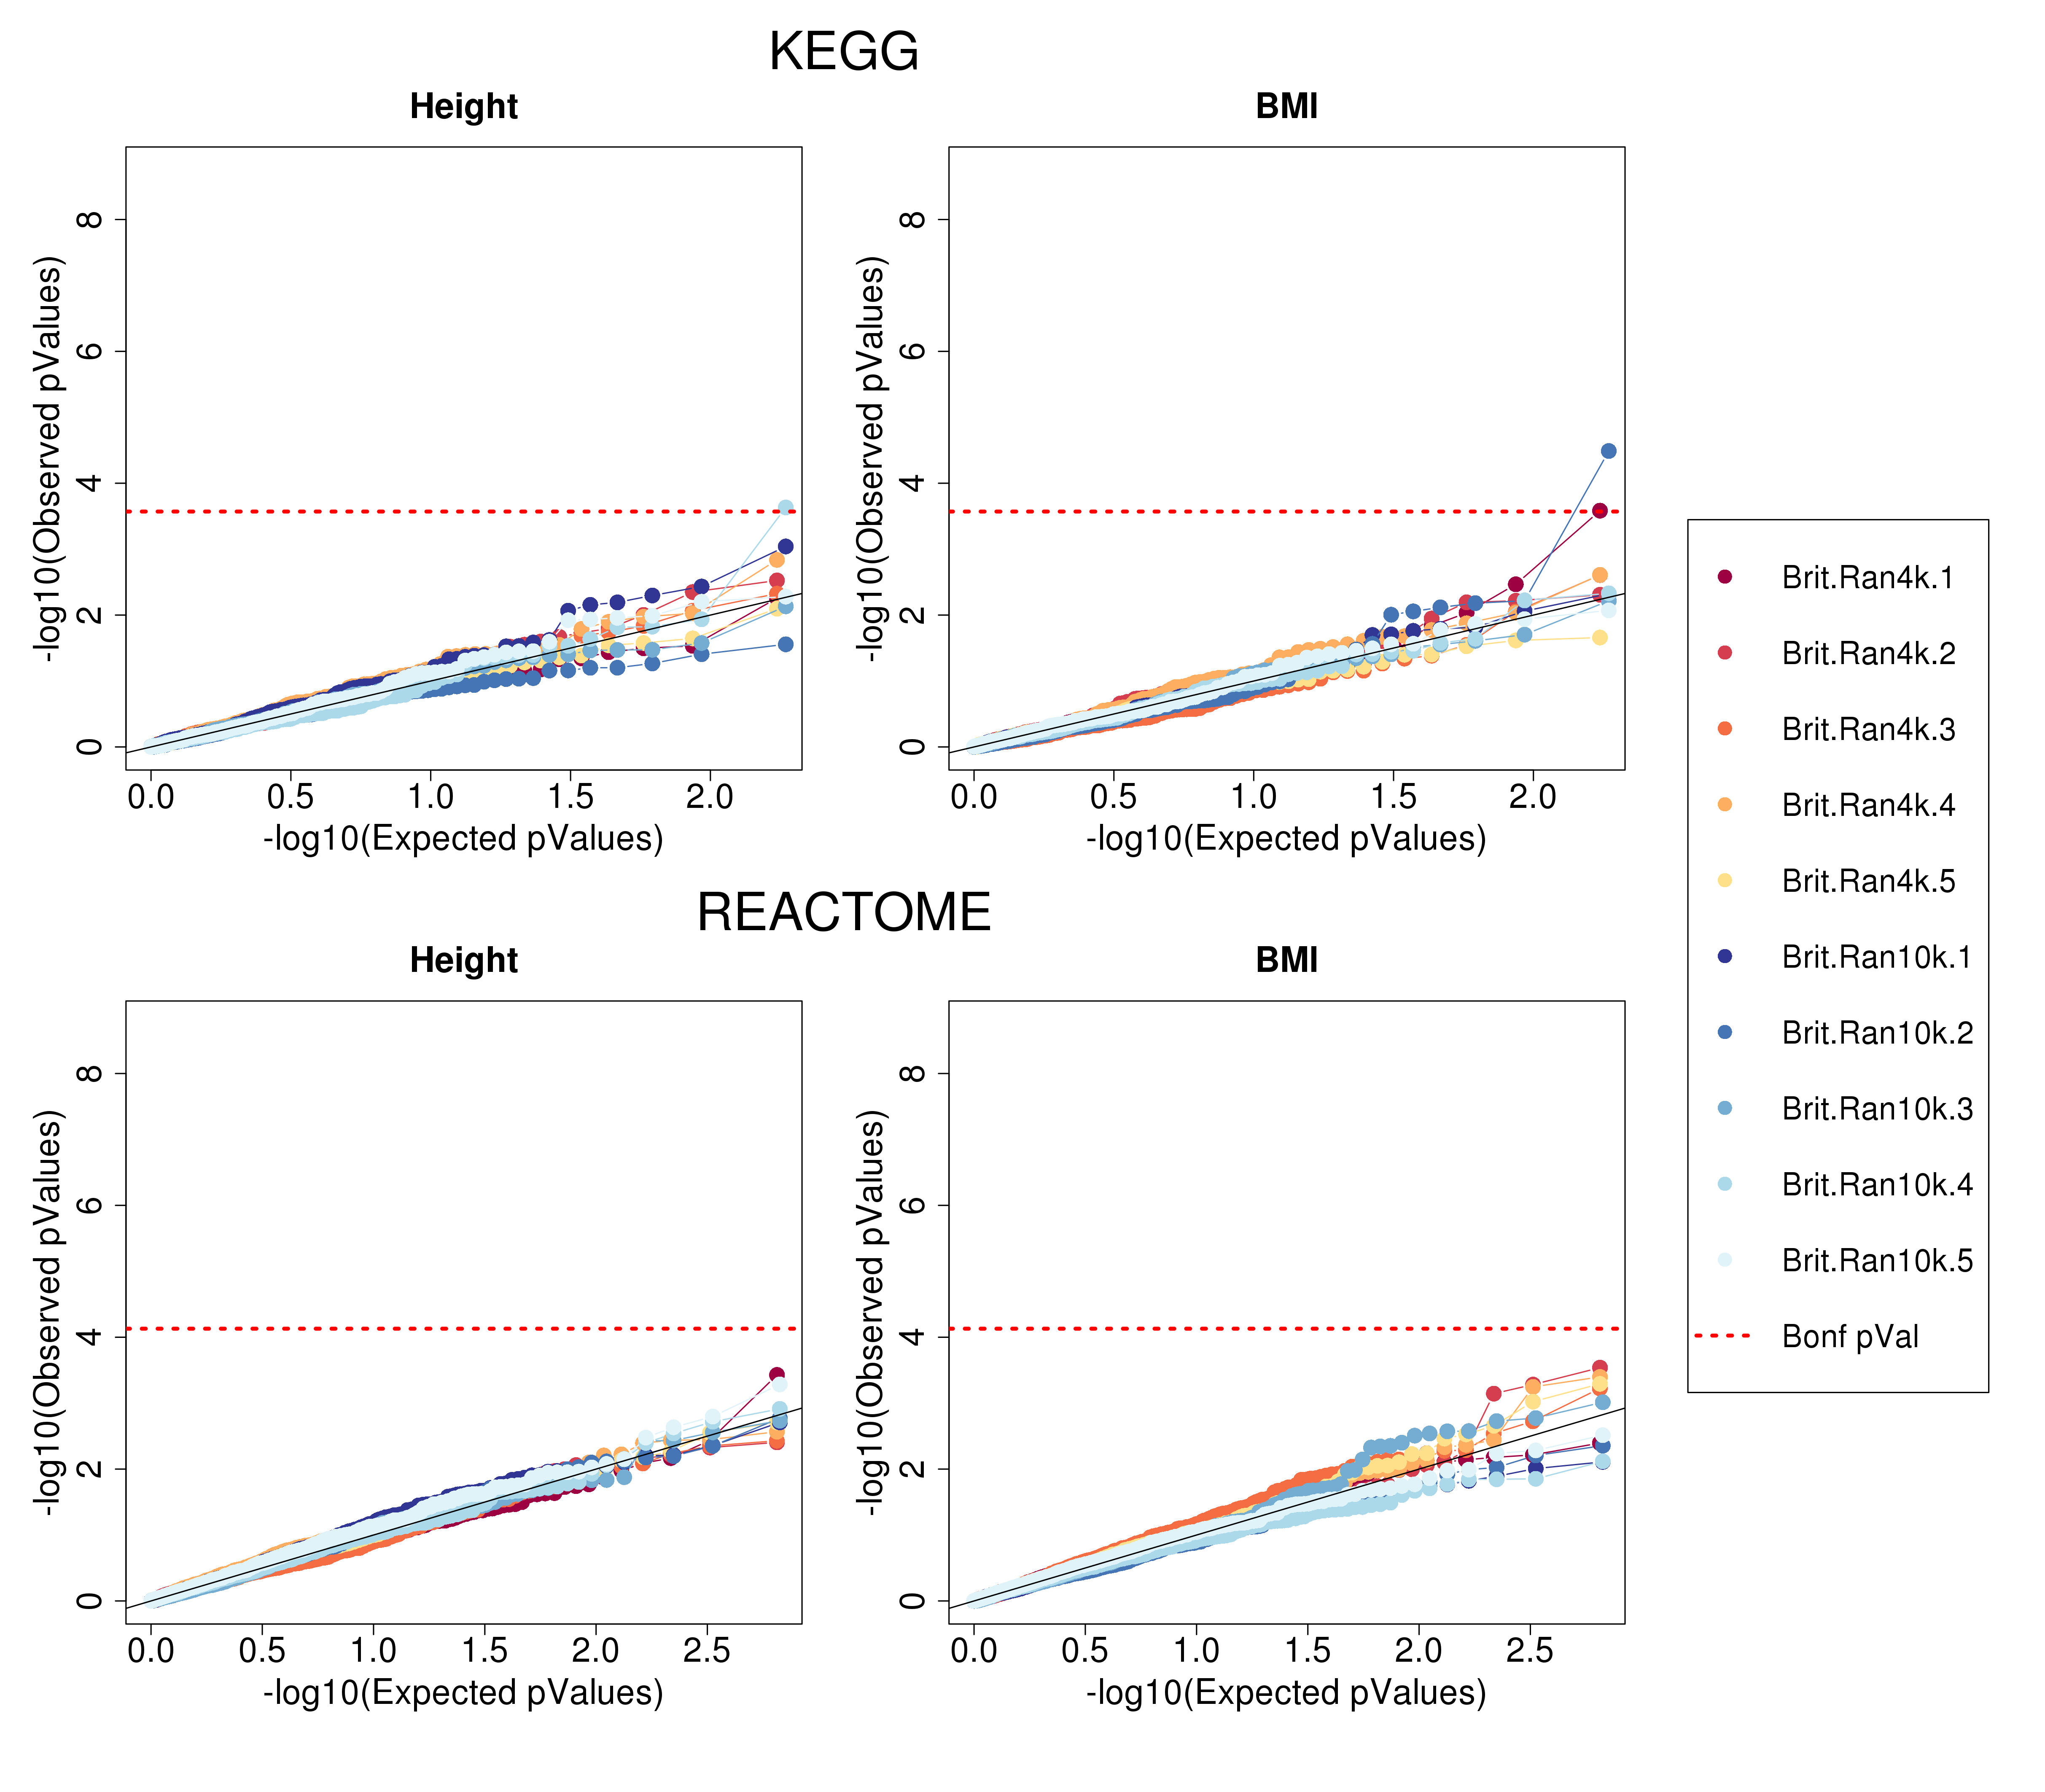
\includegraphics[scale=.35]{Images/Supp/InterPath_Supp_Figure_BritReps_perm1_QQPlots_AllPaths_vs1.png}
\caption[TBD]{\textbf{QQ-Plots of MAPIT-R results using permuted phenotypes, per British replicate}. The figure shows QQ-plots for running MAPIT-R using single, permuted versions of both height and BMI with the KEGG \& REACTOME databases. Phenotypes were permuted within each British replicate subset. Shown on the $x$-axis are the -$\log_{10}$ of the expected $p$-values and the on the $y$-axis are on the -$\log_{10}$ of the observed $p$-values. The dotted red line is our Bonferroni-corrected $p$-value threshold based on the number of pathways tested per phenotype and pathway database combination. We find across all replicate, phenotype, and pathway database combinations that MAPIT-R continues to show proper null behavior within the range expected when using permuted phenotypes.}
\label{InterPath-Supp-Figure-BritReps-perm1-QQPlots-AllPaths}
\end{figure}
\clearpage

\newcounter{CharNumber3}
\setcounter{CharNumber3}{1}
%\renewcommand{\thefigure}{\arabic{figure}\alph{CharNumber3}}
\setlength{\footskip}{1cm}
\begin{figure}[htbp]
\centering
\vspace*{-1cm}
\includegraphics[scale=.2]{Images/Supp/InterPath_Supp_Figure_BritReps_pValHists_AllPaths_vs1_pt1.png}
\caption[TBD]{\textbf{$p$-Value histograms of MAPIT-R results using permuted phenotypes, per British replicate}. The figure shows histograms of MAPIT-R $p$-values collected across ten independent phenotype permutation runs for each British Ran4000 and Ran10000 subsample replicate. The same phenotype permutation for a given replicate was used across both pathway databases (i.e. 10 permutations were done for height and 10 done for BMI for each subset). Covariates used from the original MAPIT-R analysis were kept the same.}
\label{InterPath-Supp-Figure-BritReps-10perms-pValHists-pt1}
\end{figure}
\clearpage
\setlength{\footskip}{1cm}
\addtocounter{figure}{-1}
\addtocounter{CharNumber3}{1}

\setlength{\footskip}{2cm}
\begin{figure}[htbp]
\centering
\vspace*{-1cm}
\includegraphics[scale=.2]{Images/Supp/InterPath_Supp_Figure_BritReps_pValHists_AllPaths_vs1_pt2.png}
\caption[TBD]{\textbf{$p$-Value histograms of MAPIT-R results using permuted phenotypes, per British replicate}. The figure shows histograms of MAPIT-R $p$-values collected across ten independent phenotype permutation runs for each British Ran4000 and Ran10000 subsample replicate. The same phenotype permutation for a given replicate was used across both pathway databases (i.e. 10 permutations were done for height and 10 done for BMI for each subset). Covariates used from the original MAPIT-R analysis were kept the same.}
\label{InterPath-Supp-Figure-BritReps-10perms-pValHists-pt2}
\end{figure}
\clearpage
\setlength{\footskip}{1cm}
%\renewcommand{\thefigure}{\arabic{figure}}

\begin{figure}[htbp]
\centering
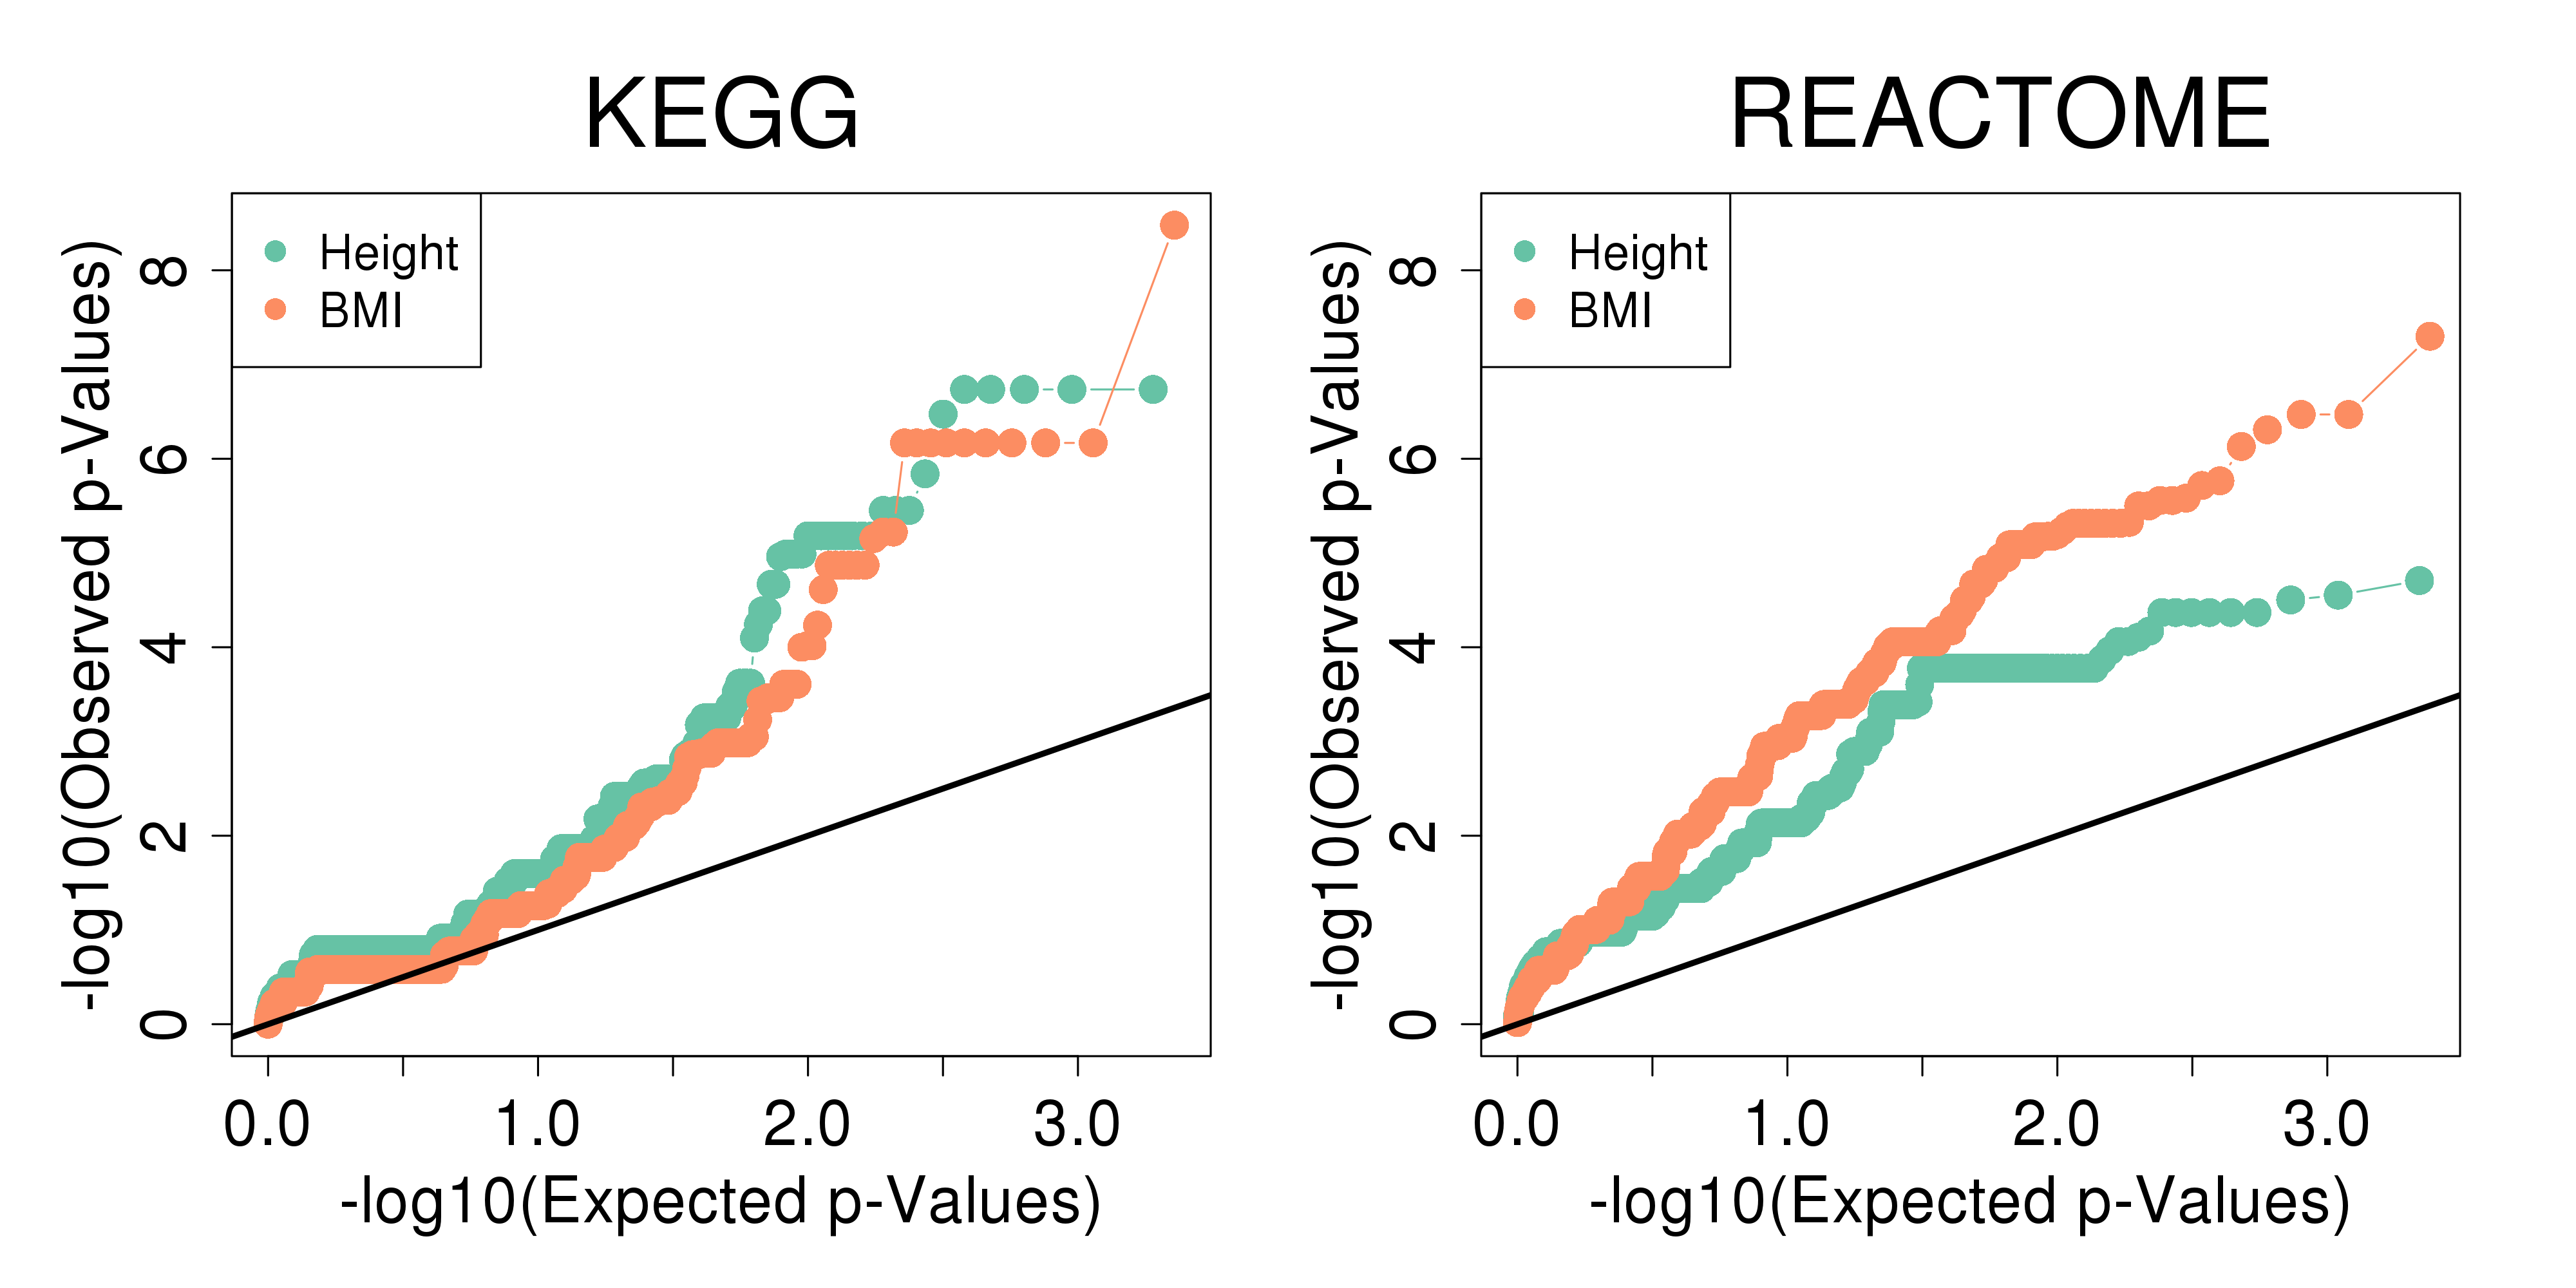
\includegraphics[scale=.45]{Images/Supp/InterPath_Supp_Figure_Hypergeometric_QQPlots_African_vs2.png}
\caption[TBD]{\textbf{QQ-Plots of gene count hypergeometric enrichment test $p$-values in the African subset}. The figure shows QQ-plots of the gene count hypergeometric enrichment results for the African subset in both height and BMI and across both the KEGG and REACTOME databases. Every gene that was present among the set of MAPIT-R genome-wide significant pathways for that phenotype and pathway database combination was tested, including genes that were only present once. The $x$-axis is the expected -$\log_{10}$ $p$-values and the $y$-axis is the observed -$\log_{10}$ $p$-values. Brown dots are results from the height analysis and purple dots are results from the BMI analysis.}
\label{InterPath-Supp-Figure-Hypergeometric-QQPlots-African}
\end{figure}
\clearpage

\begin{figure}[htbp]
\centering
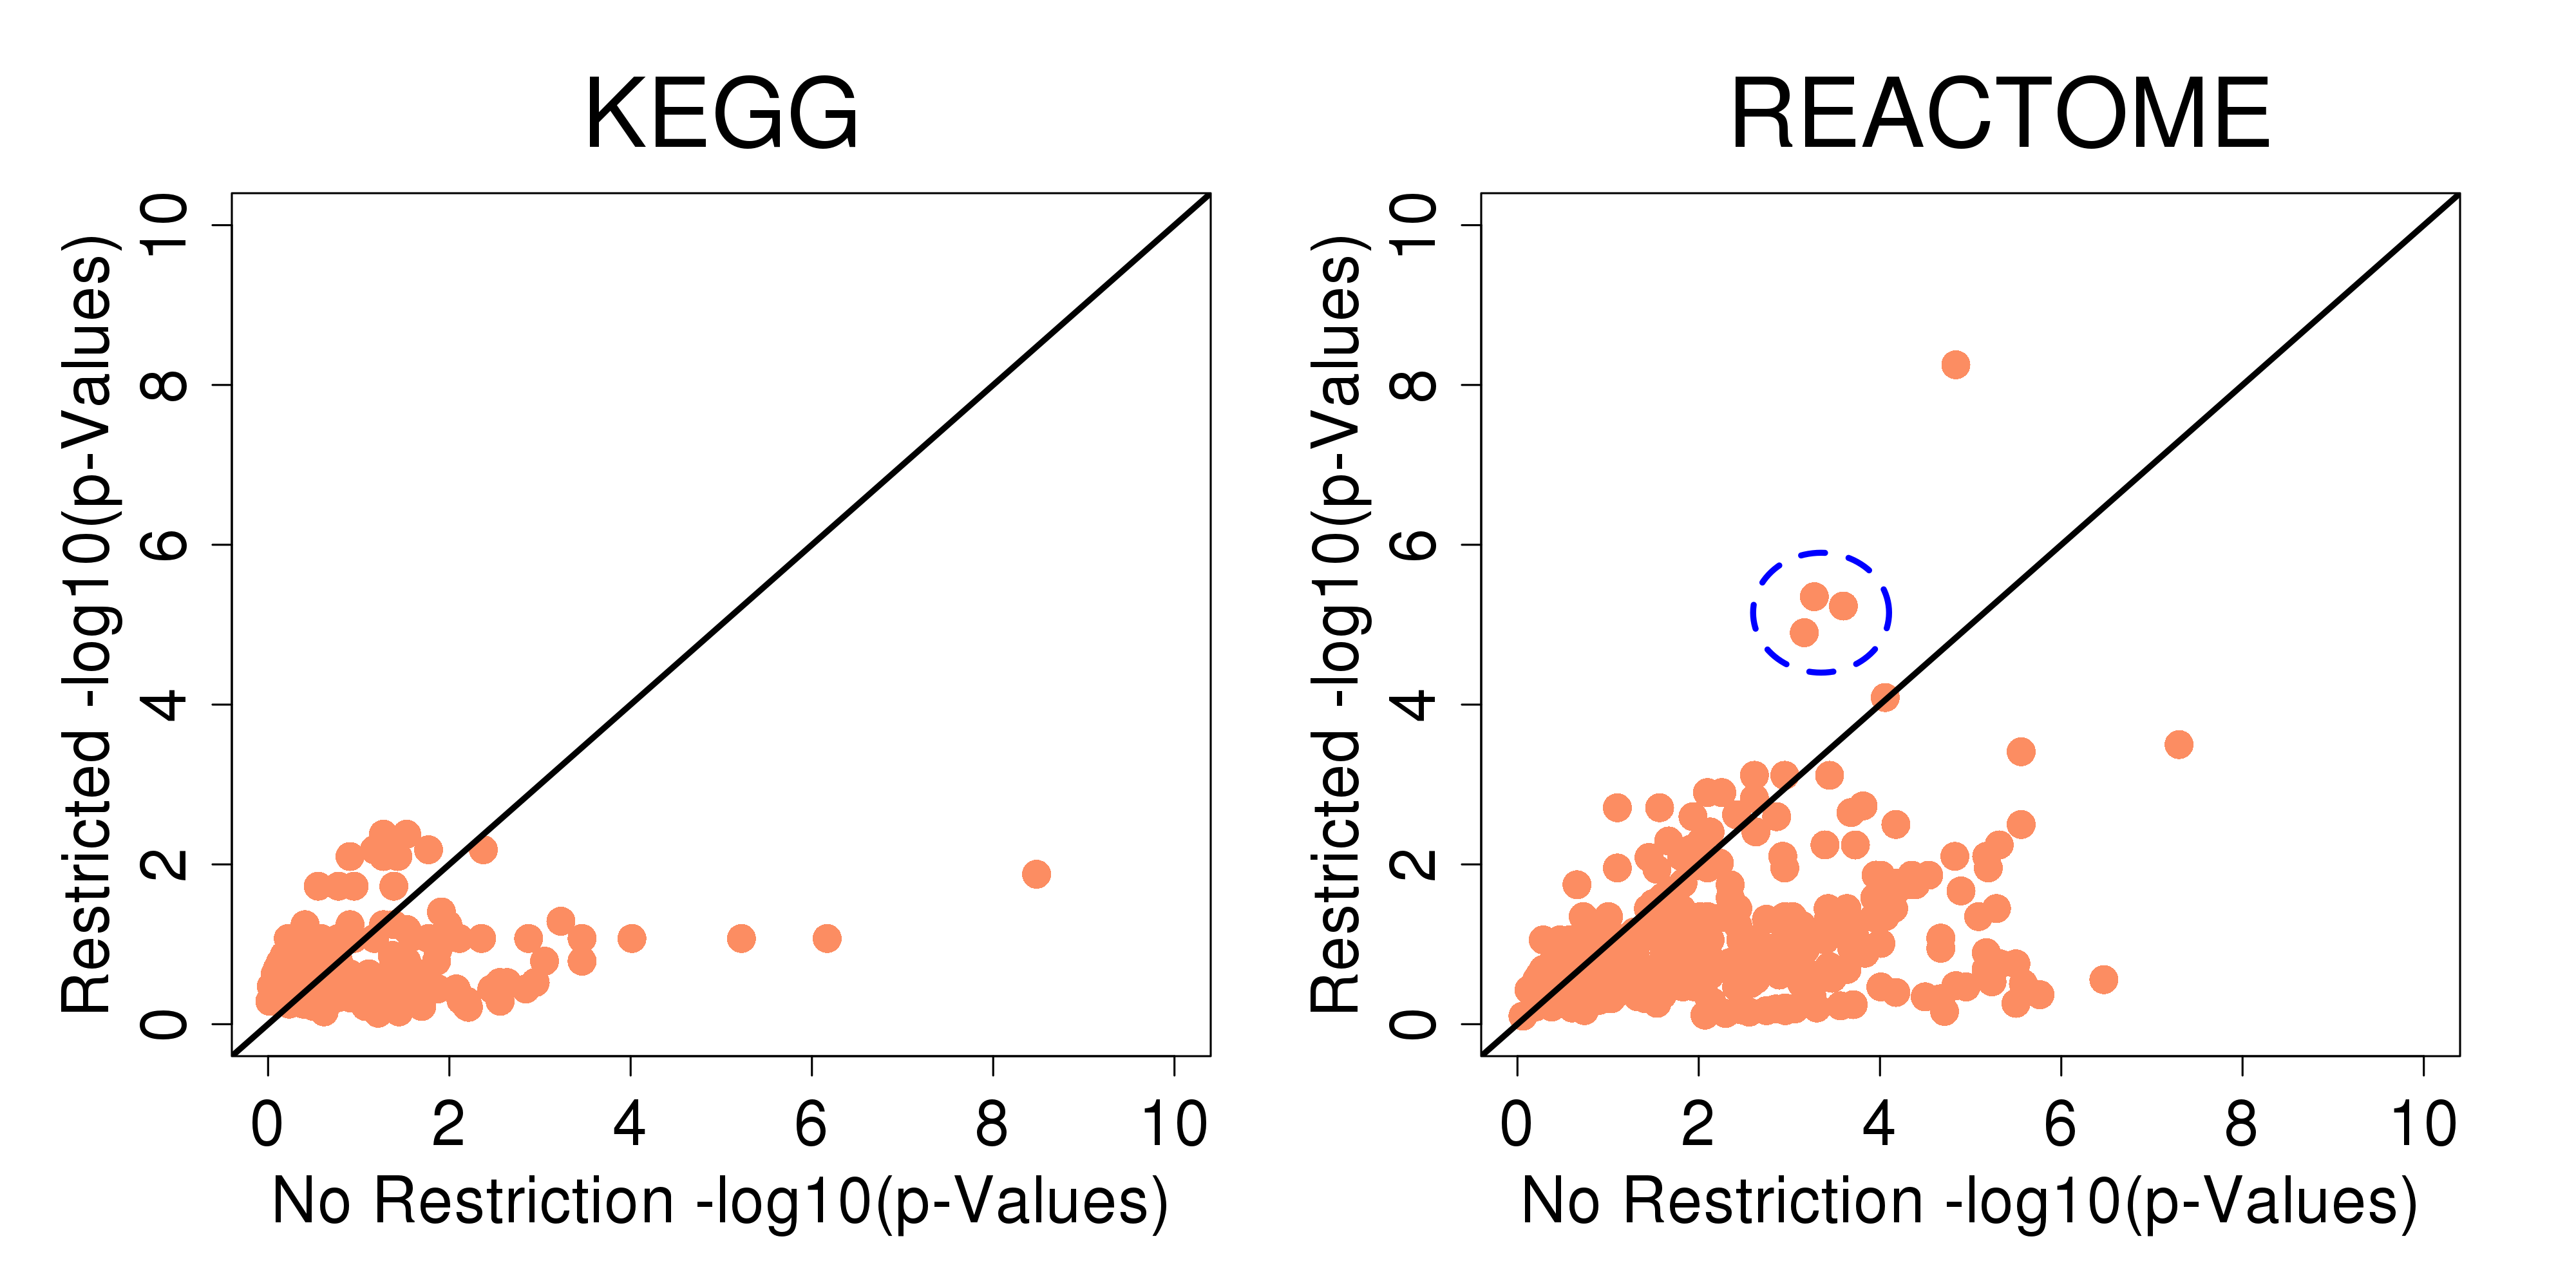
\includegraphics[scale=.45]{Images/Supp/InterPath_Supp_Figure_Hypergeometric_RestrictedComps_African_BMI_vs2.png}
\caption[TBD]{\textbf{Comparison of gene count hypergeometric enrichment $p$-values in BMI using pathway size restrictions versus no size restrictions in the African subset}. The figure shows comparisons of the gene count hypergeometric enrichment $p$-values between the size restricted version of the analysis and the original unrestricted version of the analysis. The size restricted version of the analysis is redoing the hypergeometric enrichment tests but only using pathways that contained $<=$ 1,000 SNPs. Only results for BMI are shown here since almost all Bonferroni significant pathways were lost in the height results due to this size restriction step. The $x$-axis shows the original, unrestricted hypergeometric -$\log_{10}$ $p$-values, and the $y$-axis shows the new, size restricted hypergeoemtric -$\log_{10}$ $p$-values. The PSM* gene cluster is highlighted in the REACTOME plot. For lists of the top genes that became more significant due to the size restriction step, see Supplementary Table \ref{InterPath-Supp-Table-Hypergeometric-RestrictedComps-African-BMI-TopExamples}.}
\label{InterPath-Supp-Figure-Hypergeometric-RestrictedComps-African-BMI}
\end{figure}
\clearpage

\setlength{\footskip}{3cm}
\begin{figure}[htbp]
\centering
\vspace*{-2cm}
\includegraphics[scale=.2]{Images/Supp/InterPath_Supp_Figure_IBS_AllPops_vs3.png}
\caption[TBD]{\textbf{Pathway-level genetic diversity versus MAPIT-R results for all phenotype, database, and subset combinations}. Caption continued on next page.}
\label{InterPath-Supp-Figure-IBS-AllPops}
\end{figure}
\clearpage
\setlength{\footskip}{1cm}
\addtocounter{figure}{-1}

\begin{figure} [t!]
\caption[TBD]{\textbf{Pathway-level genetic diversity versus MAPIT-R results for all phenotype, database, and subset combinations}. The figure shows the mean pairwise IBS proportions per pathway plotted against each pathway's MAPIT-R $p$-value for every UKB subset, phenotype, and pathway database combination. IBS proportions were calculated per pathway by using that pathway's set of SNPs, were calculated pairwise between every set of individuals in the subset, and then averaged across each of these pairs for a final, single summary metric. We observe across almost every combination no significant relationship between mean pairwise IBS proportion and MAPIT-R $p$-value.}
\label{InterPath-Supp-Figure-IBS-AllPops-Caption}
\end{figure}
\clearpage

\begin{figure}[htbp]
\centering
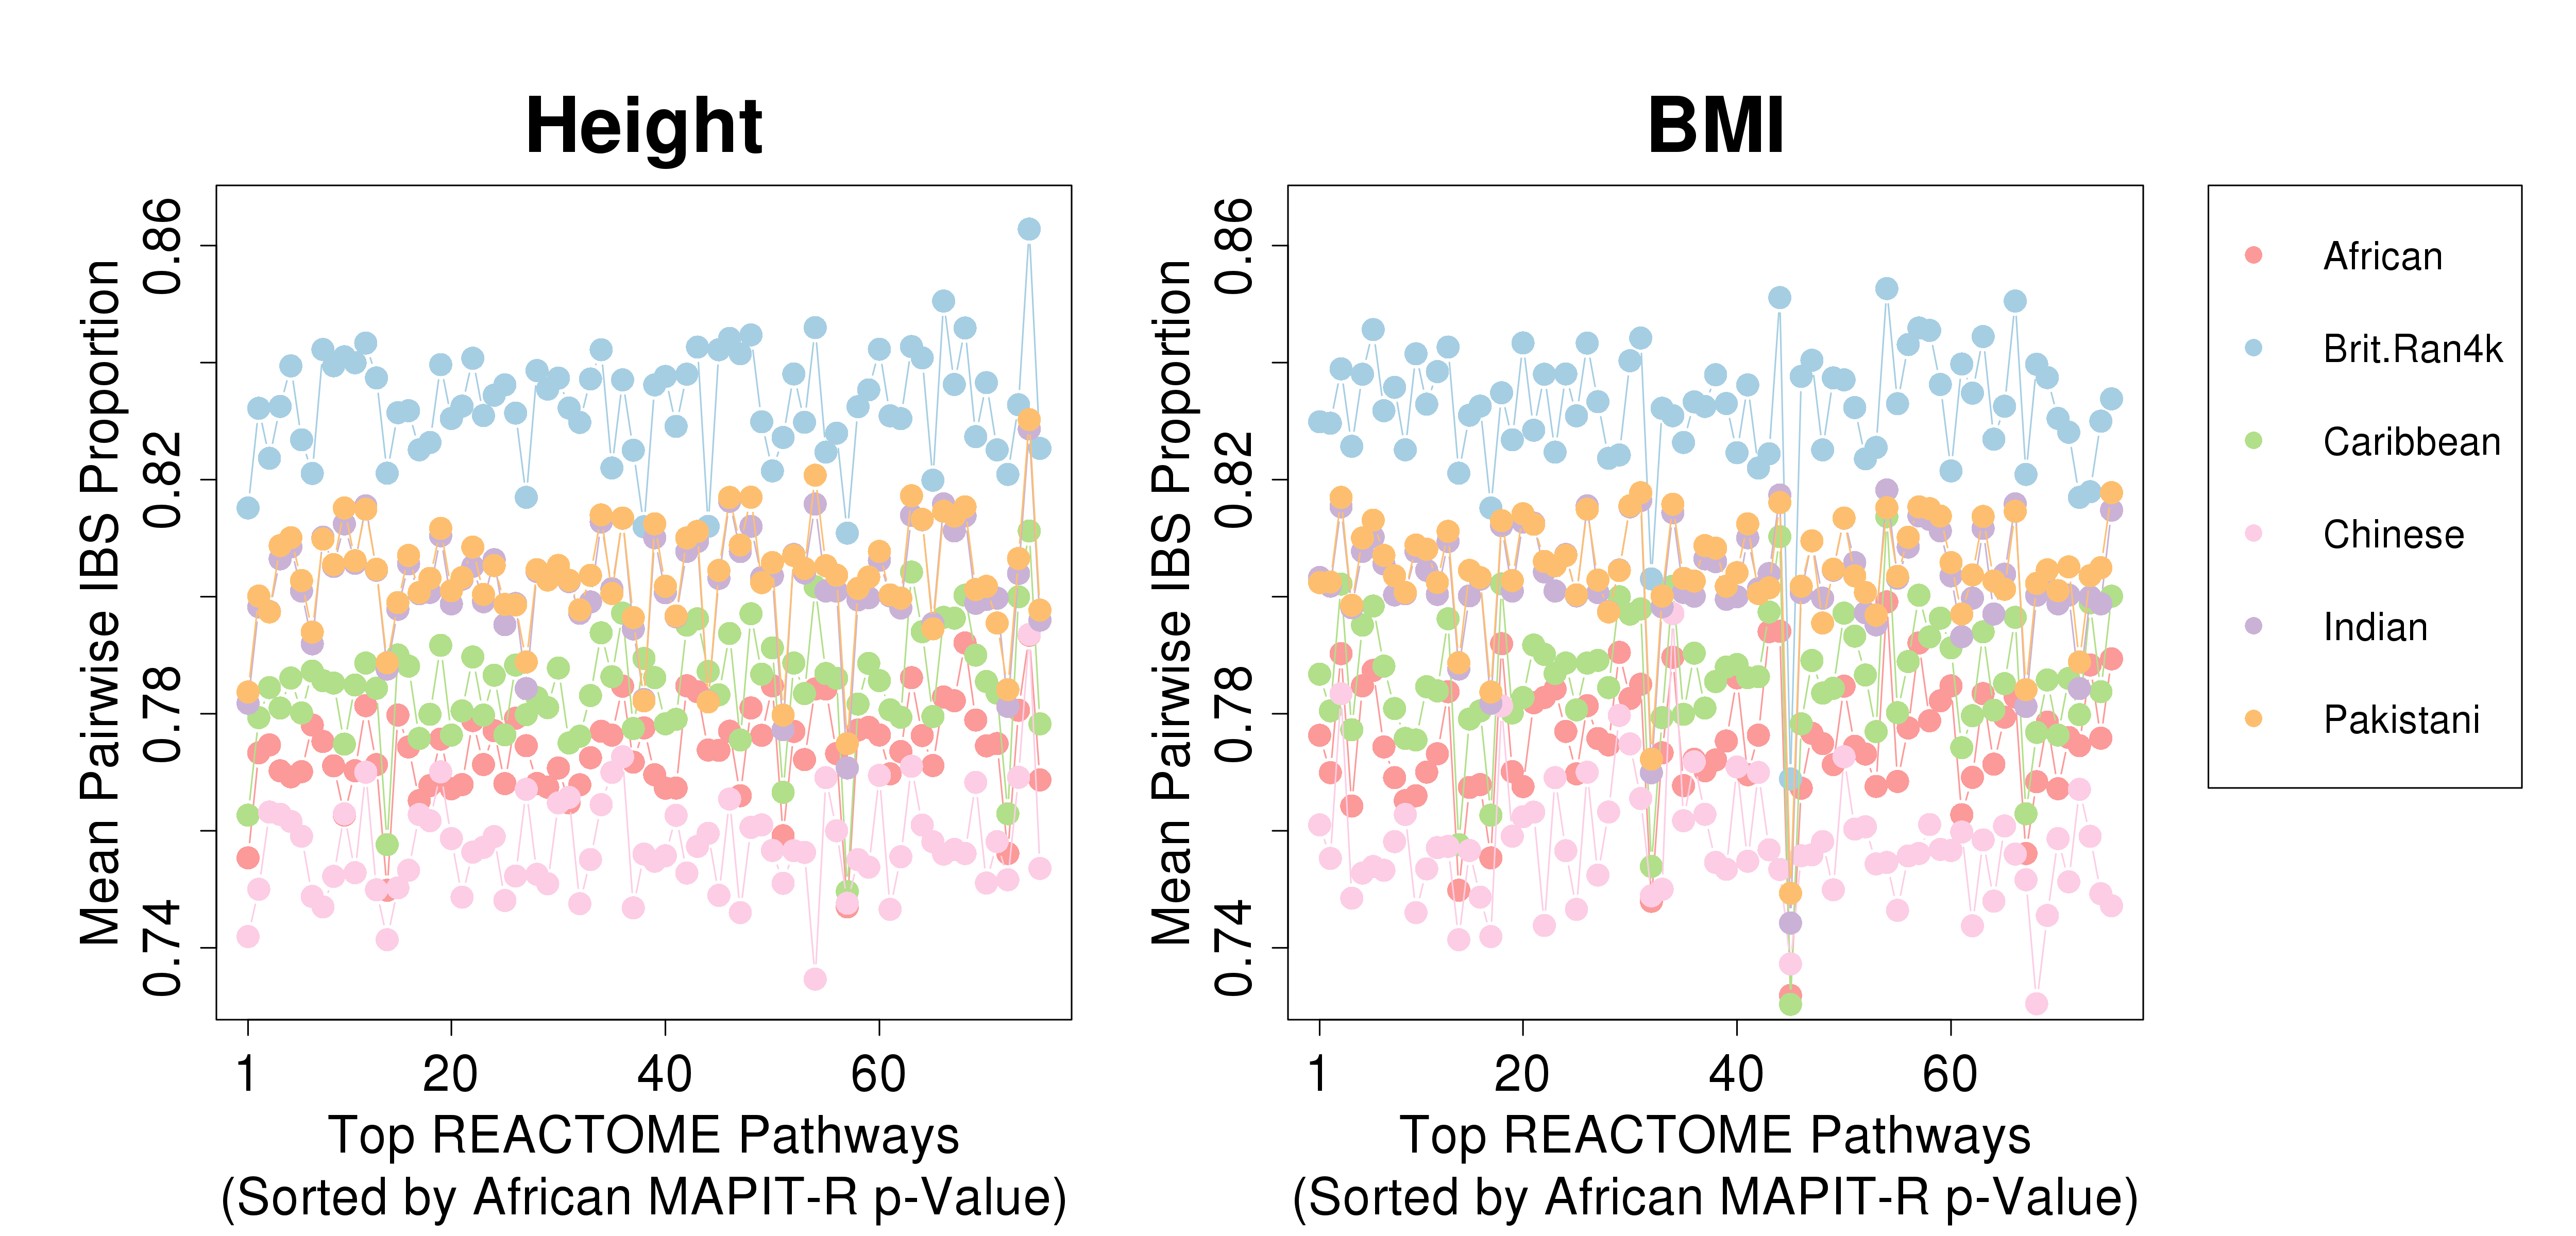
\includegraphics[scale=.35]{Images/Supp/InterPath_Supp_Figure_IBS_AllPopComps_vs3_REACTOME.png}
\caption[TBD]{\textbf{Pathway-level genetic diversity across all UKB subsets for top African MAPIT-R REACTOME pathways}. The figure plots the mean pairwise IBS proportions of each UKB subset for the top 75 REACTOME pathways (sorted by MAPIT-R African subset $p$-value) for each phenotype and pathway database combination. Most variation in mean pairwise IBS proportions varies moreso based on the pathways themselves and not on ancestry; subsets differ between one another mostly at the same levels across each pathway.}
\label{InterPath-Supp-Figure-IBS-AllPopComps-REACTOME}
\end{figure}
\clearpage

\section{Supplementary Tables}\label{Supplementary-Tables}

\begin{table}[ht]
\centering
\begin{tabular}{ccccc}
  \hline
\textbf{UK BioBank} & \textbf{Individuals} & \textbf{SNPs} & \textbf{KEGG} & \textbf{REACTOME} \\
\textbf{Subset} & & & \textbf{Pathways} & \textbf{Pathways}  \\
  \hline
\textbf{Original Subsets:} & & & & \\
African & 3111 & 374466 & 180 & 658 \\ 
British.Ran4000 & 3848 & 600006 & 173 & 650 \\ 
Caribbean & 3833 & 410017 & 181 & 661 \\ 
Chinese & 1448 & 345221 & 153 & 626 \\ 
Indian & 5077 & 505854 & 181 & 662 \\ 
Pakistani & 1581 & 516806 & 141 & 596 \\ 
\\
\textbf{British Replicates:} & & & & \\
British.Ran4000.2 & 3869 & 599381 & 173 & 650 \\ 
British.Ran4000.3 & 3836 & 600654 & 173 & 649 \\ 
British.Ran4000.4 & 3838 & 599829 & 173 & 650 \\ 
British.Ran4000.5 & 3853 & 599442 & 173 & 650 \\ 
British.Ran10000 & 9603 & 597298 & 186 & 669 \\ 
British.Ran10000.2 & 9628 & 597577 & 186 & 669 \\ 
British.Ran10000.3 & 9636 & 597486 & 186 & 669 \\ 
British.Ran10000.4 & 9593 & 597369 & 186 & 669 \\ 
British.Ran10000.5 & 9596 & 597507 & 186 & 669 \\ 
  \hline
\end{tabular}
\caption[TBD]{\textbf{UK BioBank subset and British replicate statistics}. The table shows various statistics for each group of UKB subsets that were analyzed in this study. `Original Subsets' refers to the multiple global human ancestries that were initially analyzed at the beginning of this study, and `British Replicates' refers specifically to the subsets that were created to analyze multiple, independent random subsamples of the UKB British cohort. The number of individuals and SNPs post quality-control used are shown in the second and third columns, and the number of KEGG and REACTOME pathways analyzed in each subset are shown in the fourth and fifth columns. Note that for the `British Replicates' subsets each group began with an independent set of either 4,000 or 10,000 individuals from the original UKB phenotype file.}
\label{InterPath-Supp-Table-UKBPopStats}
\end{table}
\clearpage

%Irish & 11575 & 588324 & 186 & 671 \\ 

\begin{landscape}
\setlength{\footskip}{2cm}
\begin{table}[ht]
\centering
\begin{tabular}{ccccccc}
  \hline
  \textbf{Trait} & \textbf{African} & & \textbf{British.Ran4k} & & \textbf{Caribbean} & \\ 
& \textbf{Chr:BP} & \textbf{Proportion} & \textbf{Chr:BP} & \textbf{Proportion} & \textbf{Chr:BP} & \textbf{Proportion} \\ 
  \hline
\textbf{Height:} & & & & & & \\
& 9:8851248 & 0.402 & 2:68593134 & 0.434 & 3:115845348 & 0.352 \\
  & 2:192167280 & 0.301 & 11:33992648 & 0.350 & 4:142116338 & 0.329 \\ 
  & 20:11424166 & 0.291 & 1:19440383 & 0.270 & 16:11185464 & 0.246 \\ 
  & 15:25999954 & 0.271 & 11:12738444 & 0.258 & 7:38160558 & 0.240 \\ 
  & 8:4275585 & 0.256 & 12:129932700 & 0.212 & 4:84952912 & 0.237 \\ 
  & 7:111551740 & 0.247 & 10:129548670 & 0.209 & 20:42387041 & 0.213 \\ 
  & 7:5894502 & 0.245 & 7:126672487 & 0.193 & 5:138942117 & 0.208 \\ 
  & 20:42387041 & 0.221 & 11:12674963 & 0.187 & 8:27895386 & 0.205 \\ 
  & 11:56631974 & 0.213 & 9:23129565 & 0.176 & 19:43701423 & 0.198 \\ 
  & 8:116901222 & 0.213 & 20:55953947 & 0.170 & 6:834751 & 0.196 \\ 
  \\
\textbf{BMI:} & & & & & & \\
& 16:26051170 & 0.230 & 2:27075505 & 0.293 & 12:99313419 & 0.319 \\ 
  & 5:172707503 & 0.228 & 1:107460560 & 0.267 & 5:70798541 & 0.284 \\ 
  & 11:2699051 & 0.208 & 21:16339852 & 0.212 & 2:34625180 & 0.273 \\ 
  & 5:16862840 & 0.207 & 2:223779979 & 0.189 & 1:221101692 & 0.266 \\ 
  & 8:48411885 & 0.202 & 2:162386309 & 0.189 & 14:51994228 & 0.235 \\ 
  & 10:133143956 & 0.198 & 2:138690969 & 0.189 & 10:131663327 & 0.234 \\ 
  & 15:93657838 & 0.192 & 16:83246883 & 0.177 & 1:56414458 & 0.225 \\ 
  & 16:55172951 & 0.191 & 13:90223042 & 0.174 & 5:93403619 & 0.220 \\ 
  & 17:32754797 & 0.184 & 13:92829268 & 0.163 & 2:177527111 & 0.219 \\ 
  & 6:1011570 & 0.168 & 6:100900508 & 0.157 & 1:85416840 & 0.218 \\
   \hline
\end{tabular}
\caption[TBD]{\textbf{Lists of SNPs with the largest proportions of marginally significant PLINK pairwise epistasis tests, per subset}. Caption continued at the end of the table.}
\label{InterPath-Supp-Table-PLINK-Proportions-TopSNPs-a}
\end{table}
\end{landscape}
\clearpage
\setlength{\footskip}{1cm}
\addtocounter{table}{-1}

\begin{landscape}
\setlength{\footskip}{2cm}
\begin{table}[ht]
\centering
\begin{tabular}{ccccccc}
  \hline
  \textbf{Trait} & \textbf{Chinese} & & \textbf{Indian} & & \textbf{Pakistani} & \\ 
& \textbf{Chr:BP} & \textbf{Proportion} & \textbf{Chr:BP} & \textbf{Proportion} & \textbf{Chr:BP} & \textbf{Proportion} \\ 
  \hline
\textbf{Height:} & & & & & & \\
& 6:74098688 & 1.025 & 8:22014852 & 0.203 & 3:25962790 & 1.015 \\
  & 7:19736280 & 0.503 & 2:135138136 & 0.190 & 11:33951568 & 0.953 \\ 
  & 17:74993606 & 0.493 & 11:55110903 & 0.190 & 1:61014885 & 0.616 \\ 
  & 7:150512307 & 0.491 & 2:181346849 & 0.180 & 18:18905020 & 0.580 \\ 
  & 7:95703904 & 0.461 & 2:181318303 & 0.167 & 12:119540062 & 0.573 \\ 
  & 17:8135061 & 0.416 & 1:159947480 & 0.159 & 8:145948440 & 0.558 \\ 
  & 19:2500027 & 0.413 & 1:18062545 & 0.157 & 22:44643912 & 0.539 \\ 
  & 7:95696930 & 0.408 & 8:86425809 & 0.153 & 5:175433876 & 0.491 \\ 
  & 8:89565212 & 0.401 & 5:44725795 & 0.151 & 11:101951678 & 0.488 \\ 
  & 14:86697878 & 0.399 & 5:167366400 & 0.149 & 12:119554751 & 0.486 \\
  \\
\textbf{BMI:} & & & & & & \\
& 3:74946238 & 0.692 & 6:131708393 & 0.169 & 1:24690676 & 0.872 \\ 
  & 17:65485380 & 0.689 & 11:90267176 & 0.166 & 2:30702842 & 0.458 \\ 
  & 3:116001766 & 0.496 & 3:75936499 & 0.165 & 7:29191481 & 0.448 \\ 
  & 3:30814425 & 0.470 & 5:73129149 & 0.162 & 4:167120342 & 0.431 \\ 
  & 5:117528365 & 0.395 & 13:74840677 & 0.153 & 18:45616828 & 0.411 \\ 
  & 3:75050057 & 0.370 & 12:68110089 & 0.150 & 15:90686924 & 0.406 \\ 
  & 20:55362831 & 0.354 & 11:92390082 & 0.146 & 11:131792814 & 0.391 \\ 
  & 22:22359389 & 0.338 & 4:63750280 & 0.142 & 5:83958603 & 0.379 \\ 
  & 10:85864069 & 0.332 & 18:10853771 & 0.141 & 7:152693740 & 0.375 \\ 
  & 3:75064460 & 0.320 & 16:6860576 & 0.140 & 10:110657497 & 0.371 \\ 
   \hline
\end{tabular}
\caption[TBD]{\textbf{Lists of SNPs with the largest proportions of marginally significant PLINK pairwise epistasis tests, per subset}. Caption continued at the end of the table.}
\label{InterPath-Supp-Table-PLINK-Proportions-TopSNPs-b}
\end{table}
\end{landscape}
\clearpage
\setlength{\footskip}{1cm}
\addtocounter{table}{-1}

\begin{table} [t!]
  \caption{\textbf{Lists of SNPs with the largest proportions of marginally significant PLINK pairwise epistasis tests, per subset}. The table shows the top 10 SNPs in terms of proportion of marginally significant PLINK pairwise epistatic interactions for height and BMI in each of our UKB subsets. Marginal significance is determined by a PLINK pairwise SNP interaction $p$-value being below $1\times10^{-4}$. For each UKB subset the first column lists the chromosome and basepair position for the SNP of interest and the second column lists the PLINK test proportions.}
\label{InterPath-Supp-Table-PLINK-Proportions-TopSNPs-Caption}
\end{table}
\clearpage

\begin{landscape}
\setlength{\footskip}{2cm}
\begin{table}[ht]
\centering
\begin{tabular}{ccccccc}
  \hline
  \textbf{Trait} & \textbf{African} & & \textbf{British.Ran4k} & & \textbf{Caribbean} & \\ 
& \textbf{Chr:BP} & \textbf{-$\log_{10}$($p$)} & \textbf{Chr:BP} & \textbf{-$\log_{10}$($p$)} & \textbf{Chr:BP} & \textbf{-$\log_{10}$($p$)} \\ 
  \hline
\textbf{Height:} & & & & & & \\
& 15:98255395 & 6.064 & 15:40308859 & 5.654 & 10:102705058 & 6.366 \\ 
  & 21:33179371 & 5.947 & 20:18929160 & 5.206 & 10:102754238 & 6.167 \\ 
  & 7:107441154 & 5.633 & 2:68593134 & 5.175 & 11:60876561 & 5.899 \\ 
  & 22:50883961 & 5.292 & 15:40284523 & 4.941 & 10:102738551 & 5.787 \\ 
  & 20:10633313 & 5.234 & 17:34817693 & 4.866 & 2:29225504 & 5.778 \\ 
  & 7:28263825 & 5.221 & 17:34833820 & 4.863 & 10:102746503 & 5.736 \\ 
  & 15:43423327 & 4.928 & 11:33992648 & 4.859 & 4:38155825 & 5.631 \\ 
  & 7:12077909 & 4.794 & 13:37130549 & 4.778 & 12:28230120 & 5.494 \\ 
  & 6:75947027 & 4.764 & 13:23471815 & 4.750 & 8:32275265 & 5.380 \\ 
  & 1:49180331 & 4.763 & 4:46199808 & 4.641 & 16:78704199 & 5.296 \\ 
   \\
\textbf{BMI:} & & & & & & \\
& 16:54243548 & 6.119 & 4:153811650 & 5.119 & 1:177923440 & 6.536 \\ 
  & 18:24501383 & 5.818 & 18:20190795 & 5.068 & 16:21710678 & 5.922 \\ 
  & 2:233554499 & 5.402 & 1:104061746 & 5.063 & 9:130479233 & 5.843 \\ 
  & 3:10899881 & 5.345 & 4:153690842 & 4.901 & 4:8332861 & 5.702 \\ 
  & 18:68624629 & 5.330 & 8:107630040 & 4.877 & 22:39830123 & 5.652 \\ 
  & 2:5257185 & 5.048 & 21:21535472 & 4.866 & 5:123252456 & 5.564 \\ 
  & 10:48485976 & 4.868 & 11:127409790 & 4.780 & 6:35705892 & 5.445 \\ 
  & 11:19838292 & 4.850 & 1:183277665 & 4.779 & 1:234364335 & 5.419 \\ 
  & 5:172707503 & 4.715 & 2:122598583 & 4.779 & 2:66821247 & 5.396 \\ 
  & 4:38789675 & 4.713 & 20:5478313 & 4.773 & 1:221101692 & 5.379 \\ 
   \hline
\end{tabular}
\caption[TBD]{\textbf{Lists of SNPs with the most significant MAPIT $p$-values, per subset}. Caption continued at the end of the table.}
\label{InterPath-Supp-Table-MAPIT-TopSNPs-a}
\end{table}
\end{landscape}
\clearpage
\setlength{\footskip}{1cm}
\addtocounter{table}{-1}

\begin{landscape}
\setlength{\footskip}{2cm}
\begin{table}[ht]
\centering
\begin{tabular}{ccccccc}
  \hline
  \textbf{Trait} & \textbf{Chinese} & & \textbf{Indian} & & \textbf{Pakistani} & \\ 
& \textbf{Chr:BP} & \textbf{-$\log_{10}$($p$)} & \textbf{Chr:BP} & \textbf{-$\log_{10}$($p$)} & \textbf{Chr:BP} & \textbf{-$\log_{10}$($p$)} \\ 
  \hline
\textbf{Height:} & & & & & & \\
& 4:101070872 & 5.673 & 11:30478524 & 5.869 & 14:84654448 & 5.562 \\ 
  & 9:84390158 & 5.453 & 11:30452281 & 5.546 & 2:177358580 & 4.986 \\ 
  & 19:2500027 & 5.329 & 11:30564908 & 5.443 & 2:64556555 & 4.814 \\ 
  & 13:20836940 & 5.224 & 10:121732871 & 5.399 & 6:52476643 & 4.774 \\ 
  & 4:159328540 & 5.073 & 5:151876334 & 5.351 & 3:9071220 & 4.767 \\ 
  & 10:45368032 & 4.979 & 19:53154530 & 5.304 & 6:14814367 & 4.740 \\ 
  & 6:113595727 & 4.927 & 13:19745579 & 5.223 & 1:168609132 & 4.631 \\ 
  & 4:101059291 & 4.773 & 5:158867212 & 5.198 & 16:61560661 & 4.626 \\ 
  & 10:72763749 & 4.682 & 12:32084875 & 5.138 & 7:80071426 & 4.625 \\ 
  & 3:187622081 & 4.619 & 6:46375132 & 5.120 & 8:60021908 & 4.586 \\ 
   \\
\textbf{BMI:} & & & & & & \\
& 11:97016249 & 5.184 & 2:2116870 & 6.096 & 22:25096704 & 5.147 \\ 
  & 10:12681042 & 4.961 & 8:65989176 & 6.025 & 17:12707766 & 4.907 \\ 
  & 21:34354062 & 4.809 & 6:29702709 & 5.920 & 7:10580190 & 4.778 \\ 
  & 4:14390603 & 4.736 & 6:29700079 & 5.729 & 10:73300992 & 4.744 \\ 
  & 4:14386866 & 4.643 & 6:29700615 & 5.729 & 13:42116031 & 4.652 \\ 
  & 7:73145015 & 4.642 & 4:102205385 & 5.634 & 19:13980805 & 4.402 \\ 
  & 4:14390228 & 4.618 & 7:29413388 & 5.440 & 15:25980875 & 4.350 \\ 
  & 4:14385522 & 4.587 & 3:54409526 & 5.431 & 3:32802690 & 4.328 \\ 
  & 10:122226568 & 4.586 & 8:130332722 & 5.341 & 5:133848660 & 4.304 \\ 
  & 1:33714603 & 4.576 & 8:4656695 & 5.210 & 6:40366427 & 4.296 \\ 
   \hline
\end{tabular}
\caption[TBD]{\textbf{Lists of SNPs with the most significant MAPIT $p$-values, per subset}. Caption continued at the end of the table.}
\label{InterPath-Supp-Table-MAPIT-TopSNPs-b}
\end{table}
\end{landscape}
\clearpage
\setlength{\footskip}{1cm}
\addtocounter{table}{-1}

\begin{table} [t!]
  \caption{\textbf{Lists of SNPs with the most significant MAPIT $p$-values, per subset}. The table shows the top 10 SNPs for each of our MAPIT analyses on height and BMI in our UKB subsets. For each UKB subset the first column lists the chromosome and basepair position for the SNP of interest and the second column lists the MAPIT -$\log_{10}$ $p$-value for that SNP. No single SNP reaches genome-wide significance ($p$-value $<= 5\times10^{-8}$).}
\label{InterPath-Supp-Table-MAPIT-TopSNPs-Caption}
\end{table}
\clearpage

%From: https://tex.stackexchange.com/questions/118606/numbering-tables-a1-a2-etc-in-latex & https://tex.stackexchange.com/questions/83689/next-subsequent-letter-in-the-alphabet
\newcounter{CharNumber1}
\setcounter{CharNumber1}{1}
\renewcommand{\thetable}{\arabic{table}\alph{CharNumber1}}
\setlength{\footskip}{2cm}
\begin{landscape}
\begin{table}[ht]
\centering
\vspace*{-.75cm}
\begin{tabular}{lccc}
  \hline
\textbf{Population \& Pathway} & \textbf{Genes} & \textbf{SNPs} & \textbf{$p$-Value} \\ 
  \hline
  \textbf{African:} & & & \\
 KEGG\_CHEMOKINE\_SIGNALING\_PATHWAY & 170 & 2448 & 5.136E-10 \\
 KEGG\_AXON\_GUIDANCE & 120 & 3045 & 1.511E-08 \\ 
  KEGG\_HYPERTROPHIC\_CARDIOMYOPATHY\_HCM & 77 & 2132 & 1.542E-08 \\ 
  KEGG\_CYTOKINE\_CYTOKINE\_RECEPTOR\_INTERACTION & 234 & 2279 & 2.837E-08 \\ 
  KEGG\_PURINE\_METABOLISM & 135 & 2411 & 1.186E-07 \\ 
  KEGG\_DILATED\_CARDIOMYOPATHY & 83 & 2234 & 1.242E-07 \\ 
  KEGG\_TYPE\_I\_DIABETES\_MELLITUS & 38 & 1659 & 1.330E-07 \\ 
  KEGG\_ENDOCYTOSIS & 169 & 2981 & 1.523E-07 \\ 
  KEGG\_OLFACTORY\_TRANSDUCTION & 365 & 3110 & 1.194E-06 \\ 
  KEGG\_AUTOIMMUNE\_THYROID\_DISEASE & 48 & 1504 & 1.492E-06 \\ 
  KEGG\_NATURAL\_KILLER\_CELL\_MEDIATED\_CYTOTOXICITY & 127 & 2216 & 5.160E-06 \\ 
  KEGG\_ALZHEIMERS\_DISEASE & 136 & 1846 & 5.188E-06 \\ 
  KEGG\_WNT\_SIGNALING\_PATHWAY & 141 & 2050 & 6.536E-06 \\ 
  KEGG\_ALLOGRAFT\_REJECTION & 32 & 1329 & 8.152E-06 \\ 
  KEGG\_HUNTINGTONS\_DISEASE & 148 & 1660 & 8.639E-06 \\ 
  KEGG\_GRAFT\_VERSUS\_HOST\_DISEASE & 35 & 1348 & 8.933E-06 \\ 
  KEGG\_GAP\_JUNCTION & 85 & 1851 & 9.300E-06 \\ 
  KEGG\_SYSTEMIC\_LUPUS\_ERYTHEMATOSUS & 111 & 1525 & 1.499E-05 \\ 
  KEGG\_VIRAL\_MYOCARDITIS & 64 & 1972 & 1.889E-05 \\ 
  KEGG\_ANTIGEN\_PROCESSING\_AND\_PRESENTATION & 74 & 1598 & 2.890E-05 \\ 
  KEGG\_LONG\_TERM\_POTENTIATION & 63 & 1585 & 3.317E-05 \\ 
  KEGG\_INTESTINAL\_IMMUNE\_NETWORK\_FOR\_IGA\_PRODUCTION & 43 & 1072 & 3.838E-05 \\ 
  KEGG\_PHOSPHATIDYLINOSITOL\_SIGNALING\_SYSTEM & 75 & 1681 & 4.497E-05 \\ 
  KEGG\_ARRHYTHMOGENIC\_RIGHT\_VENTRICULAR\_CARDIOMYOPATHY\_ARVC & 70 & 2373 & 5.289E-05 \\ 
  KEGG\_LONG\_TERM\_DEPRESSION & 66 & 1741 & 5.553E-05 \\ 
  KEGG\_GLIOMA & 64 & 974 & 5.649E-05 \\ 
  KEGG\_VASCULAR\_SMOOTH\_MUSCLE\_CONTRACTION & 106 & 2465 & 1.881E-04 \\ 
  KEGG\_REGULATION\_OF\_ACTIN\_CYTOSKELETON & 194 & 3047 & 1.951E-04 \\ 
  KEGG\_TYPE\_II\_DIABETES\_MELLITUS & 45 & 979 & 2.687E-04 \\ 
   \hline
\end{tabular}
\caption[TBD]{\textbf{Lists of genome-wide significant MAPIT-R KEGG pathways in height, per subset}. Caption continued at end of tables.}
\label{InterPath-Supp-Table-TopPathways-KEGG-Height-a}
\end{table}
\addtocounter{table}{-1}
%\addtocounter{CharNumber1}{1}
\clearpage

\begin{table}[ht]
\centering
\vspace*{-.75cm}
\begin{tabular}{lccc}
  \hline
  \textbf{British.Ran4000:} & & & \\
  KEGG\_ERBB\_SIGNALING\_PATHWAY & 83 & 2674 & 1.003E-05 \\
KEGG\_TYPE\_I\_DIABETES\_MELLITUS &  39 & 1924 & 1.693E-05 \\ 
 \textcolor{white}{KEGG\_ARRHYTHMOGENIC\_RIGHT\_VENTRICULAR\_CARDIOMYOPATHY\_ARVC } & & & \\
 \textbf{Caribbean:} & & & \\
 KEGG\_CHEMOKINE\_SIGNALING\_PATHWAY & 171 & 2688 & 2.733E-06 \\
 KEGG\_NATURAL\_KILLER\_CELL\_MEDIATED\_CYTOTOXICITY & 128 & 2356 & 1.125E-05 \\
  KEGG\_CELL\_ADHESION\_MOLECULES\_CAMS & 120 & 4029 & 1.770E-05 \\
  KEGG\_LEUKOCYTE\_TRANSENDOTHELIAL\_MIGRATION & 105 & 1941 & 2.169E-05 \\
  KEGG\_VASCULAR\_SMOOTH\_MUSCLE\_CONTRACTION & 106 & 2708 & 3.675E-05 \\
  KEGG\_AXON\_GUIDANCE & 120 & 3365 & 1.088E-04 \\
  KEGG\_SMALL\_CELL\_LUNG\_CANCER & 78 & 1931 & 1.369E-04 \\
  KEGG\_ARRHYTHMOGENIC\_RIGHT\_VENTRICULAR\_CARDIOMYOPATHY\_ARVC & 70 & 2581 & 1.376E-04 \\
  KEGG\_HYPERTROPHIC\_CARDIOMYOPATHY\_HCM & 77 & 2298 & 1.960E-04 \\
 \\
 \textbf{Chinese:} & & & \\
 KEGG\_TYPE\_I\_DIABETES\_MELLITUS & 39 & 1573 & 1.269E-08 \\
 KEGG\_ANTIGEN\_PROCESSING\_AND\_PRESENTATION & 75 & 1505 & 8.287E-08 \\
  KEGG\_MELANOGENESIS & 96 & 1382 & 1.028E-05 \\
  KEGG\_ALLOGRAFT\_REJECTION & 33 & 1250 & 1.183E-05 \\
  KEGG\_GRAFT\_VERSUS\_HOST\_DISEASE & 37 & 1274 & 2.424E-05 \\
  KEGG\_NON\_SMALL\_CELL\_LUNG\_CANCER & 53 & 1081 & 5.337E-05 \\
  KEGG\_SYSTEMIC\_LUPUS\_ERYTHEMATOSUS & 109 & 1399 & 1.252E-04 \\
 \\
 \textbf{Indian:} & & & \\
 KEGG\_NON\_SMALL\_CELL\_LUNG\_CANCER & 53 & 1696 & 4.182E-05 \\
 KEGG\_CYTOKINE\_CYTOKINE\_RECEPTOR\_INTERACTION & 237 & 2995 & 4.965E-05 \\
  KEGG\_REGULATION\_OF\_ACTIN\_CYTOSKELETON & 193 & 4069 & 1.963E-04 \\
  KEGG\_ERBB\_SIGNALING\_PATHWAY & 83 & 2174 & 2.128E-04 \\
   \hline
\end{tabular}
\caption[TBD]{\textbf{Lists of genome-wide significant MAPIT-R KEGG pathways in height, per subset}. Continued. \\ }
\label{InterPath-Supp-Table-TopPathways-KEGG-Height-b}
\end{table}
\addtocounter{table}{-1}
%\addtocounter{CharNumber1}{1}

\begin{table}[ht]
\centering
\vspace*{-.75cm}
\begin{tabular}{lccc}
  \hline
 \textbf{Pakistani:} & & & \\
 KEGG\_ANTIGEN\_PROCESSING\_AND\_PRESENTATION & 78 & 1775 & 1.581E-08 \\
 KEGG\_AMINO\_SUGAR\_AND\_NUCLEOTIDE\_SUGAR\_METABOLISM & 40 & 610 & 7.840E-05 \\
  KEGG\_AUTOIMMUNE\_THYROID\_DISEASE & 49 & 1680 & 2.602E-04 \\
 \\
   \hline
\end{tabular}
\caption[TBD]{\textbf{Lists of genome-wide significant MAPIT-R KEGG pathways in height, per subset}. Continued. \\ }
\label{InterPath-Supp-Table-TopPathways-KEGG-Height-c}
\end{table}
\addtocounter{table}{-1}
\clearpage

%\end{landscape}
%\begin{table} [t!]
%  \caption{\textbf{Genome-Wide Significant MAPIT-R Pathways: KEGG Height}. The tables show the lists of KEGG pathways for each subset that were found to be MAPIT-R genome-wide significant for height. Genome-wide significance was determined by using a Bonferroni-corrected $p$-value threshold of .05 divided by the number of pathways tested. The first column lists the subsets and KEGG pathways, the second column lists the number of genes that were included in the MAPIT-R test, the third column lists the number of SNPs that were included in the MAPIT-R test, and the fourth column lists the MAPIT-R $p$-values.}
%\label{InterPath-Supp-Table-TopPathways-KEGG-Height-Caption}
%\end{table}
%\addtocounter{table}{-1}
%\addtocounter{CharNumber1}{1}
%\clearpage
%\begin{landscape}

\begin{table}[ht]
\centering
\vspace*{-.75cm}
\begin{tabular}{lccc}
  \hline
\textbf{Population \& Pathway} & \textbf{Genes} & \textbf{SNPs} & \textbf{$p$-Value} \\ 
  \hline
  \textbf{African:} & & & \\
  KEGG\_AXON\_GUIDANCE & 120 & 3045 & 0.000E+00 \\
 KEGG\_SMALL\_CELL\_LUNG\_CANCER & 78 & 1776 & 3.199E-10 \\
  KEGG\_TYPE\_I\_DIABETES\_MELLITUS & 38 & 1659 & 4.291E-10 \\
  KEGG\_REGULATION\_OF\_ACTIN\_CYTOSKELETON & 194 & 3047 & 8.253E-10 \\
  KEGG\_AUTOIMMUNE\_THYROID\_DISEASE & 48 & 1504 & 1.393E-08 \\
  KEGG\_CHEMOKINE\_SIGNALING\_PATHWAY & 170 & 2448 & 1.512E-08 \\
  KEGG\_ALLOGRAFT\_REJECTION & 32 & 1329 & 2.529E-08 \\
  KEGG\_GRAFT\_VERSUS\_HOST\_DISEASE & 35 & 1348 & 4.753E-08 \\
  KEGG\_NATURAL\_KILLER\_CELL\_MEDIATED\_CYTOTOXICITY & 127 & 2216 & 1.081E-07 \\
  KEGG\_WNT\_SIGNALING\_PATHWAY & 141 & 2050 & 1.414E-07 \\
  KEGG\_SYSTEMIC\_LUPUS\_ERYTHEMATOSUS & 111 & 1525 & 1.504E-07 \\
  KEGG\_HYPERTROPHIC\_CARDIOMYOPATHY\_HCM & 77 & 2132 & 1.578E-07 \\
  KEGG\_ANTIGEN\_PROCESSING\_AND\_PRESENTATION & 74 & 1598 & 2.075E-07 \\
  KEGG\_ERBB\_SIGNALING\_PATHWAY & 83 & 1538 & 3.298E-07 \\
  KEGG\_OLFACTORY\_TRANSDUCTION & 365 & 3110 & 8.627E-07 \\
  KEGG\_GAP\_JUNCTION & 85 & 1851 & 8.996E-07 \\
  KEGG\_VIRAL\_MYOCARDITIS & 64 & 1972 & 1.086E-06 \\
  KEGG\_ARRHYTHMOGENIC\_RIGHT\_VENTRICULAR\_CARDIOMYOPATHY\_ARVC & 70 & 2373 & 1.581E-06 \\
  KEGG\_NON\_SMALL\_CELL\_LUNG\_CANCER & 53 & 1243 & 1.640E-06 \\
  KEGG\_JAK\_STAT\_SIGNALING\_PATHWAY & 138 & 1324 & 2.000E-06 \\
  KEGG\_PURINE\_METABOLISM & 135 & 2411 & 2.463E-06 \\
  KEGG\_GLIOMA & 64 & 974 & 3.564E-06 \\
  KEGG\_T\_CELL\_RECEPTOR\_SIGNALING\_PATHWAY & 102 & 1373 & 6.120E-06 \\
  KEGG\_DILATED\_CARDIOMYOPATHY & 83 & 2234 & 6.987E-06 \\
  KEGG\_ENDOCYTOSIS & 169 & 2981 & 8.023E-06 \\
  KEGG\_ALZHEIMERS\_DISEASE & 136 & 1846 & 8.567E-06 \\
  KEGG\_TYPE\_II\_DIABETES\_MELLITUS & 45 & 979 & 8.598E-06 \\
  KEGG\_HUNTINGTONS\_DISEASE & 148 & 1660 & 1.310E-05 \\
  KEGG\_VALINE\_LEUCINE\_AND\_ISOLEUCINE\_DEGRADATION & 41 & 399 & 1.710E-05 \\
   \hline
\end{tabular}
\caption[TBD]{\textbf{Lists of genome-wide significant MAPIT-R KEGG pathways in BMI, per subset}. Caption continued at end of tables.}
\label{InterPath-Supp-Table-TopPathways-KEGG-BMI-a}
\end{table}
\addtocounter{table}{-1}
%\addtocounter{CharNumber1}{1}

\begin{table}[ht]
\centering
\vspace*{-.75cm}
\begin{tabular}{lccc}
  \hline
  KEGG\_ADHERENS\_JUNCTION & 66 & 1603 & 2.023E-05 \\
  KEGG\_VASCULAR\_SMOOTH\_MUSCLE\_CONTRACTION & 106 & 2465 & 2.410E-05 \\
  KEGG\_LONG\_TERM\_POTENTIATION & 63 & 1585 & 2.624E-05 \\
  KEGG\_INTESTINAL\_IMMUNE\_NETWORK\_FOR\_IGA\_PRODUCTION & 43 & 1072 & 2.987E-05 \\
  KEGG\_P53\_SIGNALING\_PATHWAY & 63 & 527 & 3.529E-05 \\
  KEGG\_NEUROTROPHIN\_SIGNALING\_PATHWAY & 117 & 1483 & 7.897E-05 \\
  KEGG\_BETA\_ALANINE\_METABOLISM & 20 & 295 & 1.127E-04 \\
  KEGG\_ECM\_RECEPTOR\_INTERACTION & 81 & 2116 & 1.185E-04 \\
  KEGG\_ETHER\_LIPID\_METABOLISM & 28 & 337 & 1.406E-04 \\
  KEGG\_LEISHMANIA\_INFECTION & 64 & 1353 & 1.441E-04 \\
  KEGG\_CELL\_CYCLE & 115 & 858 & 1.484E-04 \\
  KEGG\_INOSITOL\_PHOSPHATE\_METABOLISM & 53 & 849 & 1.534E-04 \\
  KEGG\_LEUKOCYTE\_TRANSENDOTHELIAL\_MIGRATION & 105 & 1786 & 1.633E-04 \\
  KEGG\_HOMOLOGOUS\_RECOMBINATION & 22 & 248 & 1.749E-04 \\
  KEGG\_O\_GLYCAN\_BIOSYNTHESIS & 25 & 575 & 1.923E-04 \\
  KEGG\_MELANOGENESIS & 98 & 1516 & 1.971E-04 \\
  KEGG\_ASTHMA & 26 & 850 & 2.636E-04 \\
  KEGG\_PROSTATE\_CANCER & 85 & 1143 & 2.640E-04 \\
  \\
  \textbf{British.Ran4000:} & & & \\
  KEGG\_NATURAL\_KILLER\_CELL\_MEDIATED\_CYTOTOXICITY & 128 & 3133 & 2.205E-06 \\
  KEGG\_TYPE\_I\_DIABETES\_MELLITUS & 39 & 1924 & 2.335E-05 \\
  KEGG\_ANTIGEN\_PROCESSING\_AND\_PRESENTATION & 79 & 1728 & 3.659E-05 \\
  KEGG\_JAK\_STAT\_SIGNALING\_PATHWAY & 139 & 2076 & 1.139E-04 \\
 \textcolor{white}{KEGG\_ARRHYTHMOGENIC\_RIGHT\_VENTRICULAR\_CARDIOMYOPATHY\_ARVC } & & & \\
 \textbf{Caribbean:} & & & \\
 KEGG\_CHEMOKINE\_SIGNALING\_PATHWAY & 171 & 2688 & 1.086E-06 \\
 KEGG\_CYTOKINE\_CYTOKINE\_RECEPTOR\_INTERACTION & 237 & 2453 & 4.294E-06 \\
  KEGG\_ARRHYTHMOGENIC\_RIGHT\_VENTRICULAR\_CARDIOMYOPATHY\_ARVC & 70 & 2581 & 2.070E-05 \\
   KEGG\_AXON\_GUIDANCE & 120 & 3365 & 2.382E-05 \\
  KEGG\_OLFACTORY\_TRANSDUCTION & 366 & 3318 & 5.058E-05 \\
   \hline
\end{tabular}
\caption[TBD]{\textbf{Lists of genome-wide significant MAPIT-R KEGG pathways in BMI, per subset}. Continued. \\ }
\label{InterPath-Supp-Table-TopPathways-KEGG-BMI-b}
\end{table}
\addtocounter{table}{-1}
%\addtocounter{CharNumber1}{1}

\begin{table}[ht]
\centering
\vspace*{-.75cm}
\begin{tabular}{lccc}
  \hline
  KEGG\_REGULATION\_OF\_ACTIN\_CYTOSKELETON & 193 & 3340 & 9.265E-05 \\
  KEGG\_VASCULAR\_SMOOTH\_MUSCLE\_CONTRACTION & 106 & 2708 & 1.374E-04 \\
  \\
 \textbf{Chinese:} & & & \\
 KEGG\_ANTIGEN\_PROCESSING\_AND\_PRESENTATION & 75 & 1505 & 4.430E-09 \\
 KEGG\_SYSTEMIC\_LUPUS\_ERYTHEMATOSUS & 109 & 1399 & 4.766E-07 \\
  KEGG\_LEISHMANIA\_INFECTION & 65 & 1263 & 1.224E-06 \\
  KEGG\_VIRAL\_MYOCARDITIS & 65 & 1808 & 2.157E-06 \\
  KEGG\_ALLOGRAFT\_REJECTION & 33 & 1250 & 2.648E-05 \\
  KEGG\_FC\_EPSILON\_RI\_SIGNALING\_PATHWAY & 76 & 1241 & 4.929E-05 \\
  KEGG\_TYPE\_I\_DIABETES\_MELLITUS & 39 & 1573 & 7.376E-05 \\
  KEGG\_GRAFT\_VERSUS\_HOST\_DISEASE & 37 & 1274 & 1.049E-04 \\
  \textcolor{white}{KEGG\_ARRHYTHMOGENIC\_RIGHT\_VENTRICULAR\_CARDIOMYOPATHY\_ARVC } & & & \\
 \textbf{Indian:} & & & \\
 KEGG\_ENDOCYTOSIS & 170 & 4003 & 8.651E-09 \\
 KEGG\_CYTOKINE\_CYTOKINE\_RECEPTOR\_INTERACTION & 237 & 2995 & 9.500E-05 \\
  KEGG\_REGULATION\_OF\_ACTIN\_CYTOSKELETON & 193 & 4069 & 1.034E-04 \\
  KEGG\_ERBB\_SIGNALING\_PATHWAY & 83 & 2174 & 1.827E-04 \\
 \\
 \textbf{Pakistani:} & & & \\
 KEGG\_GRAFT\_VERSUS\_HOST\_DISEASE & 37 & 1466 & 5.412E-06 \\
 KEGG\_ANTIGEN\_PROCESSING\_AND\_PRESENTATION & 78 & 1775 & 6.724E-06 \\
  KEGG\_ALLOGRAFT\_REJECTION & 33 & 1442 & 1.214E-05 \\
  KEGG\_AUTOIMMUNE\_THYROID\_DISEASE & 49 & 1680 & 1.978E-05 \\
  KEGG\_MELANOMA & 68 & 1352 & 8.436E-05 \\
 \\
   \hline
\end{tabular}
\caption[TBD]{\textbf{Lists of genome-wide significant MAPIT-R KEGG pathways in BMI, per subset}. Continued. \\ }
\label{InterPath-Supp-Table-TopPathways-KEGG-BMI-c}
\end{table}
\addtocounter{table}{-1}
\clearpage

%\end{landscape}
%\begin{table} [t!]
%  \caption{\textbf{Genome-Wide Significant MAPIT-R Pathways: KEGG BMI}. The tables show the lists of KEGG pathways for each subset that were found to be MAPIT-R genome-wide significant for BMI. Genome-wide significance was determined by using a Bonferroni-corrected $p$-value threshold of .05 divided by the number of pathways tested. The first column lists the subsets and KEGG pathways, the second column lists the number of genes that were included in the MAPIT-R test, the third column lists the number of SNPs that were included in the MAPIT-R test, and the fourth column lists the MAPIT-R $p$-values.}
%\label{InterPath-Supp-Table-TopPathways-KEGG-BMI-Caption}
%\end{table}
%\addtocounter{table}{-1}
%\addtocounter{CharNumber1}{1}
%\clearpage
%\begin{landscape}

\begin{table}[ht]
\centering
\vspace*{-1.25cm}
\begin{tabular}{lccc}
  \hline
\textbf{Population \& Pathway} & \textbf{Genes} & \textbf{SNPs} & \textbf{$p$-Value} \\ 
  \hline
  \textbf{African:} & & & \\
  REACTOME\_GASTRIN\_CREB\_SIGNALLING\_PATHWAY\_VIA\_PKC\_AND\_MAPK & 183 & 2980 & 4.861E-10 \\
  REACTOME\_NEUROTRANSMITTER\_RECEPTOR\_BINDING\_AND\_DOWNSTREAM\_ & 125 & 2942 & 3.431E-09 \\
  \qquad TRANSMISSION\_IN\_THE\_POSTSYNAPTIC\_CELL & & & \\
  REACTOME\_SIGNALING\_BY\_RHO\_GTPASES & 96 & 2385 & 6.821E-09 \\
  REACTOME\_CLASS\_A1\_RHODOPSIN\_LIKE\_RECEPTORS & 261 & 2502 & 3.245E-08 \\
  REACTOME\_TRANSPORT\_OF\_INORGANIC\_CATIONS\_ANIONS\_AND\_AMINO\_ & 86 & 1511 & 6.637E-08 \\
  \qquad ACIDS\_OLIGOPEPTIDES & & & \\
  REACTOME\_CYTOKINE\_SIGNALING\_IN\_IMMUNE\_SYSTEM & 253 & 3100 & 8.416E-08 \\
  REACTOME\_INNATE\_IMMUNE\_SYSTEM & 236 & 2334 & 1.464E-07 \\
  REACTOME\_L1CAM\_INTERACTIONS & 73 & 1679 & 7.396E-07 \\
  REACTOME\_G\_ALPHA\_Q\_SIGNALLING\_EVENTS & 164 & 2636 & 8.124E-07 \\
  REACTOME\_CELL\_CYCLE & 351 & 2459 & 1.275E-06 \\
  REACTOME\_CELL\_CELL\_COMMUNICATION & 107 & 3031 & 1.685E-06 \\
  REACTOME\_HEPARAN\_SULFATE\_HEPARIN\_HS\_GAG\_METABOLISM & 43 & 1170 & 2.873E-06 \\
  REACTOME\_INTEGRIN\_CELL\_SURFACE\_INTERACTIONS & 76 & 1594 & 4.270E-06 \\
  REACTOME\_PHOSPHOLIPID\_METABOLISM & 175 & 2260 & 7.533E-06 \\
  REACTOME\_MHC\_CLASS\_II\_ANTIGEN\_PRESENTATION & 81 & 1215 & 7.852E-06 \\
  REACTOME\_SIGNALING\_BY\_PDGF & 115 & 1902 & 9.120E-06 \\
  REACTOME\_PLATELET\_HOMEOSTASIS & 71 & 1453 & 9.317E-06 \\
  REACTOME\_SIGNALING\_BY\_NOTCH & 89 & 1534 & 1.695E-05 \\
  REACTOME\_METABOLISM\_OF\_CARBOHYDRATES & 207 & 2990 & 2.512E-05 \\
  REACTOME\_SEMAPHORIN\_INTERACTIONS & 62 & 1074 & 4.253E-05 \\
  REACTOME\_TRANSPORT\_OF\_GLUCOSE\_AND\_OTHER\_SUGARS\_BILE\_SALTS\_ & 87 & 1190 & 4.679E-05 \\
  \qquad AND\_ORGANIC\_ACIDS\_METAL\_IONS\_AND\_AMINE\_COMPOUNDS & & & \\
  REACTOME\_SIGNALING\_BY\_ERBB4 & 85 & 1483 & 4.911E-05 \\
  REACTOME\_OPIOID\_SIGNALLING & 71 & 1467 & 5.233E-05 \\
  REACTOME\_CELL\_JUNCTION\_ORGANIZATION & 67 & 1701 & 7.339E-05 \\
  \\
   \textbf{British.Ran4000:} & & & \\
  NA & & & \\
   \hline
\end{tabular}
\caption[TBD]{\textbf{Lists of genome-wide significant MAPIT-R REACTOME pathways in height, per subset}. Caption continued at end of tables.}
\label{InterPath-Supp-Table-TopPathways-REACTOME-Height-a}
\end{table}
\addtocounter{table}{-1}
%\addtocounter{CharNumber1}{1}

\begin{table}[ht]
\centering
\vspace*{-.75cm}
\begin{tabular}{lccc}
  \hline
 \textbf{Caribbean:} & \textcolor{white}{Genes} & & \\
 REACTOME\_CLASS\_A1\_RHODOPSIN\_LIKE\_RECEPTORS & 263 & 2699 & 1.853E-07 \\
 REACTOME\_METABOLISM\_OF\_CARBOHYDRATES & 206 & 3283 & 7.116E-06 \\
  REACTOME\_SIGNALING\_BY\_RHO\_GTPASES & 97 & 2635 & 9.553E-06 \\
  REACTOME\_INTEGRATION\_OF\_ENERGY\_METABOLISM & 107 & 2158 & 1.004E-05 \\
  REACTOME\_GLYCOSAMINOGLYCAN\_METABOLISM & 97 & 2301 & 1.703E-05 \\
  REACTOME\_FACTORS\_INVOLVED\_IN\_MEGAKARYOCYTE\_DEVELOPMENT\_AND\_ & 118 & 1715 & 2.724E-05 \\
  \qquad PLATELET\_PRODUCTION & & & \\
  REACTOME\_PLATELET\_ACTIVATION\_SIGNALING\_AND\_AGGREGATION & 183 & 3354 & 5.992E-05 \\
  \textcolor{white}{REACTOME\_NEUROTRANSMITTER\_RECEPTOR\_BINDING\_AND\_DOWNSTREAM\_} & & & \\
 \textbf{Chinese:} & & & \\
 REACTOME\_MHC\_CLASS\_II\_ANTIGEN\_PRESENTATION & 82 & 1118 & 1.861E-06 \\
 REACTOME\_INTERFERON\_GAMMA\_SIGNALING & 59 & 1263 & 1.127E-05 \\
 \\
 \textbf{Indian:} & & & \\
 REACTOME\_SIGNALING\_BY\_EGFR\_IN\_CANCER & 102 & 2196 & 7.705E-06 \\
 REACTOME\_SIGNALING\_BY\_FGFR\_IN\_DISEASE & 120 & 2307 & 3.131E-05 \\
 \\
 \textbf{Pakistani:} & & & \\
 NA & & & \\
 \\
   \hline
\end{tabular}
\caption[TBD]{\textbf{Lists of genome-wide significant MAPIT-R REACTOME pathways in height, per subset}. Continued. \\ }
\label{InterPath-Supp-Table-TopPathways-REACTOME-Height-b}
\end{table}
\addtocounter{table}{-1}
\clearpage

%\end{landscape}
%\begin{table} [t!]
%  \caption{\textbf{Genome-Wide Significant MAPIT-R Pathways: REACTOME Height}. The tables show the lists of REACTOME pathways for each subset that were found to be MAPIT-R genome-wide significant for height. Genome-wide significance was determined by using a Bonferroni-corrected $p$-value threshold of .05 divided by the number of pathways tested. The first column lists the subsets and REACTOME pathways, the second column lists the number of genes that were included in the MAPIT-R test, the third column lists the number of SNPs that were included in the MAPIT-R test, and the fourth column lists the MAPIT-R $p$-values.}
%\label{InterPath-Supp-Table-TopPathways-REACTOME-Height-Caption}
%\end{table}
%\addtocounter{table}{-1}
%\addtocounter{CharNumber1}{1}
%\clearpage
%\begin{landscape}

\begin{table}[ht]
\centering
\vspace*{-1.25cm}
\begin{tabular}{lccc}
  \hline
\textbf{Population \& Pathway} & \textbf{Genes} & \textbf{SNPs} & \textbf{$p$-Value} \\ 
  \hline
  \textbf{African:} & & & \\
  REACTOME\_CYTOKINE\_SIGNALING\_IN\_IMMUNE\_SYSTEM & 253 & 3100 & 0.000E+00 \\
  REACTOME\_GASTRIN\_CREB\_SIGNALLING\_PATHWAY\_VIA\_PKC\_AND\_MAPK & 183 & 2980 & 0.000E+00 \\
  REACTOME\_G\_ALPHA\_Q\_SIGNALLING\_EVENTS & 164 & 2636 & 8.225E-09 \\
  REACTOME\_SIGNALING\_BY\_RHO\_GTPASES & 96 & 2385 & 3.098E-08 \\
  REACTOME\_INNATE\_IMMUNE\_SYSTEM & 236 & 2334 & 4.412E-08 \\
  REACTOME\_SIGNALING\_BY\_NOTCH & 89 & 1534 & 6.911E-08 \\
  REACTOME\_GLYCEROPHOSPHOLIPID\_BIOSYNTHESIS & 73 & 897 & 9.695E-08 \\
  REACTOME\_PHOSPHOLIPID\_METABOLISM & 175 & 2260 & 1.037E-07 \\
  REACTOME\_NGF\_SIGNALLING\_VIA\_TRKA\_FROM\_THE\_PLASMA\_MEMBRANE & 128 & 1957 & 1.412E-07 \\
  REACTOME\_CLASS\_B\_2\_SECRETIN\_FAMILY\_RECEPTORS & 75 & 864 & 1.758E-07 \\
  REACTOME\_SIGNALING\_BY\_PDGF & 115 & 1902 & 4.269E-07 \\
  REACTOME\_HEPARAN\_SULFATE\_HEPARIN\_HS\_GAG\_METABOLISM & 43 & 1170 & 7.242E-07 \\
  REACTOME\_HIV\_INFECTION & 171 & 1346 & 7.528E-07 \\
  REACTOME\_P75\_NTR\_RECEPTOR\_MEDIATED\_SIGNALLING & 67 & 1273 & 7.929E-07 \\
  REACTOME\_G\_ALPHA1213\_SIGNALLING\_EVENTS & 66 & 1382 & 8.905E-07 \\
  REACTOME\_SIGNALING\_BY\_ERBB2 & 95 & 1639 & 1.093E-06 \\
  REACTOME\_CELL\_CYCLE & 351 & 2459 & 1.288E-06 \\
  REACTOME\_OPIOID\_SIGNALLING & 71 & 1467 & 1.549E-06 \\
  REACTOME\_MEIOSIS & 92 & 659 & 2.306E-06 \\
  REACTOME\_CHONDROITIN\_SULFATE\_DERMATAN\_SULFATE\_METABOLISM & 41 & 1049 & 2.342E-06 \\
  REACTOME\_CELL\_CELL\_COMMUNICATION & 107 & 3031 & 2.783E-06 \\
  REACTOME\_M\_G1\_TRANSITION & 73 & 458 & 3.191E-06 \\
  REACTOME\_CLASS\_A1\_RHODOPSIN\_LIKE\_RECEPTORS & 261 & 2502 & 3.378E-06 \\
  REACTOME\_G\_ALPHA\_S\_SIGNALLING\_EVENTS & 110 & 1827 & 3.446E-06 \\
  REACTOME\_CELL\_JUNCTION\_ORGANIZATION & 67 & 1701 & 4.237E-06 \\
  REACTOME\_SIGNALING\_BY\_NOTCH1 & 61 & 1165 & 4.826E-06 \\
  REACTOME\_CELL\_CYCLE\_CHECKPOINTS & 105 & 670 & 5.781E-06 \\
  REACTOME\_PLC\_BETA\_MEDIATED\_EVENTS & 40 & 916 & 7.257E-06 \\
  REACTOME\_HOST\_INTERACTIONS\_OF\_HIV\_FACTORS & 112 & 963 & 7.521E-06 \\
   REACTOME\_NCAM1\_INTERACTIONS & 37 & 957 & 8.383E-06 \\
   \hline
\end{tabular}
\caption[TBD]{\textbf{Lists of genome-wide significant MAPIT-R REACTOME pathways in BMI, per subset}. Caption continued at end of tables.}
\label{InterPath-Supp-Table-TopPathways-REACTOME-BMI-a}
\end{table}
\addtocounter{table}{-1}
%\addtocounter{CharNumber1}{1}

\begin{table}[ht]
\centering
\vspace*{-.75cm}
\begin{tabular}{lccc}
  \hline
  REACTOME\_CD28\_CO\_STIMULATION & 31 & 421 & 8.809E-06 \\
  REACTOME\_GLYCOSAMINOGLYCAN\_METABOLISM & 97 & 2092 & 1.006E-05 \\
  REACTOME\_REGULATION\_OF\_INSULIN\_SECRETION & 81 & 1544 & 1.131E-05 \\
  REACTOME\_DOWNSTREAM\_SIGNALING\_EVENTS\_OF\_B\_CELL\_RECEPTOR\_BCR & 89 & 745 & 1.195E-05 \\
  REACTOME\_REGULATION\_OF\_APOPTOSIS & 52 & 564 & 1.218E-05 \\
  REACTOME\_FACTORS\_INVOLVED\_IN\_MEGAKARYOCYTE\_DEVELOPMENT\_AND\_ & 118 & 1560 & 1.264E-05 \\
  \qquad PLATELET\_PRODUCTION & \textcolor{white}{Genes} & & \\
  REACTOME\_MITOTIC\_G1\_G1\_S\_PHASES & 121 & 747 & 1.453E-05 \\
REACTOME\_NCAM\_SIGNALING\_FOR\_NEURITE\_OUT\_GROWTH & 61 & 1271 & 1.473E-05 \\
  REACTOME\_COSTIMULATION\_BY\_THE\_CD28\_FAMILY & 60 & 1005 & 1.745E-05 \\
  REACTOME\_ACTIVATION\_OF\_NF\_KAPPAB\_IN\_B\_CELLS & 59 & 465 & 1.861E-05 \\
  REACTOME\_HS\_GAG\_BIOSYNTHESIS & 25 & 932 & 1.901E-05 \\
  REACTOME\_MHC\_CLASS\_II\_ANTIGEN\_PRESENTATION & 81 & 1215 & 1.971E-05 \\
  REACTOME\_DOWNSTREAM\_SIGNAL\_TRANSDUCTION & 89 & 1288 & 1.980E-05 \\
  REACTOME\_MEIOTIC\_SYNAPSIS & 58 & 460 & 2.081E-05 \\
  REACTOME\_SIGNALING\_BY\_EGFR\_IN\_CANCER & 102 & 1579 & 2.106E-05 \\
  REACTOME\_POST\_NMDA\_RECEPTOR\_ACTIVATION\_EVENTS & 31 & 727 & 2.296E-05 \\
  REACTOME\_SIGNALING\_BY\_SCF\_KIT & 74 & 773 & 2.350E-05 \\
  REACTOME\_METABOLISM\_OF\_CARBOHYDRATES & 207 & 2990 & 3.003E-05 \\
  REACTOME\_HYALURONAN\_METABOLISM & 14 & 178 & 3.106E-05 \\
  REACTOME\_ASSEMBLY\_OF\_THE\_PRE\_REPLICATIVE\_COMPLEX & 60 & 331 & 3.293E-05 \\
  REACTOME\_ANTIGEN\_PROCESSING\_CROSS\_PRESENTATION & 68 & 850 & 3.956E-05 \\
  REACTOME\_NEUROTRANSMITTER\_RELEASE\_CYCLE & 30 & 631 & 4.501E-05 \\
  REACTOME\_CELL\_CYCLE\_MITOTIC & 274 & 1906 & 4.509E-05 \\
  REACTOME\_A\_TETRASACCHARIDE\_LINKER\_SEQUENCE\_IS\_REQUIRED\_FOR\_ & 21 & 570 & 4.835E-05 \\
  \qquad GAG\_SYNTHESIS & & & \\
  REACTOME\_DSCAM\_INTERACTIONS & 11 & 571 & 5.055E-05 \\  
  REACTOME\_SIGNALING\_BY\_ERBB4 & 85 & 1483 & 5.085E-05 \\
  REACTOME\_CELL\_DEATH\_SIGNALLING\_VIA\_NRAGE\_NRIF\_AND\_NADE & 50 & 1118 & 5.113E-05 \\
  REACTOME\_TRANSPORT\_OF\_GLUCOSE\_AND\_OTHER\_SUGARS\_BILE\_SALTS\_ & 87 & 1190 & 5.386E-05 \\
  \qquad AND\_ORGANIC\_ACIDS\_METAL\_IONS\_AND\_AMINE\_COMPOUNDS & & & \\
  REACTOME\_RNA\_POL\_I\_TRANSCRIPTION & 67 & 388 & 5.693E-05 \\
   \hline
\end{tabular}
\caption[TBD]{\textbf{Lists of genome-wide significant MAPIT-R REACTOME pathways in BMI, per subset}. Continued. \\ }
\label{InterPath-Supp-Table-TopPathways-REACTOME-BMI-b}
\end{table}
\addtocounter{table}{-1}
%\addtocounter{CharNumber1}{1}

\begin{table}[ht]
\centering
\vspace*{-1.25cm}
\begin{tabular}{lccc}
  \hline
   REACTOME\_INTEGRATION\_OF\_ENERGY\_METABOLISM & 107 & 1985 & 5.734E-05 \\
    REACTOME\_INTEGRIN\_CELL\_SURFACE\_INTERACTIONS & 76 & 1594 & 5.806E-05 \\
  REACTOME\_PLATELET\_HOMEOSTASIS & 71 & 1453 & 5.938E-05 \\
    REACTOME\_CHROMOSOME\_MAINTENANCE & 97 & 687 & 6.167E-05 \\
  REACTOME\_G\_ALPHA\_I\_SIGNALLING\_EVENTS & 170 & 2065 & 6.829E-05 \\
   REACTOME\_NOTCH1\_INTRACELLULAR\_DOMAIN\_REGULATES\_TRANSCRIPTION & 39 & 874 & 6.902E-05 \\
   \\
  \textbf{British.Ran4000:} & \textcolor{white}{Genes} & & \\
  REACTOME\_GLUCOSE\_METABOLISM & 53 & 783 & 7.372E-06 \\
  REACTOME\_ANTIGEN\_PROCESSING\_CROSS\_PRESENTATION & 70 & 1104 & 2.482E-05 \\
  REACTOME\_IMMUNOREGULATORY\_INTERACTIONS\_BETWEEN\_A\_LYMPHOID\_ & 57 & 1162 & 2.638E-05 \\
  \qquad AND\_A\_NON\_LYMPHOID\_CELL & & & \\
  REACTOME\_INTERFERON\_SIGNALING & 152 & 2724 & 4.265E-05 \\
 \textcolor{white}{KEGG\_ARRHYTHMOGENIC\_RIGHT\_VENTRICULAR\_CARDIOMYOPATHY\_ARVC } & & & \\
 \textbf{Caribbean:} & & & \\
 REACTOME\_PLATELET\_ACTIVATION\_SIGNALING\_AND\_AGGREGATION & 183 & 3354 & 3.255E-07 \\
  REACTOME\_METABOLISM\_OF\_CARBOHYDRATES & 206 & 3283 & 2.147E-06 \\
  REACTOME\_CLASS\_A1\_RHODOPSIN\_LIKE\_RECEPTORS & 263 & 2699 & 6.266E-06 \\
  REACTOME\_NEUROTRANSMITTER\_RECEPTOR\_BINDING\_AND\_DOWNSTREAM\_ & 125 & 3204 & 8.397E-06 \\
  \qquad TRANSMISSION\_IN\_THE\_POSTSYNAPTIC\_CELL & & & \\
  REACTOME\_GASTRIN\_CREB\_SIGNALLING\_PATHWAY\_VIA\_PKC\_AND\_MAPK & 184 & 3271 & 4.661E-05 \\
  REACTOME\_GLYCOSAMINOGLYCAN\_METABOLISM & 97 & 2301 & 4.873E-05 \\
 \\
 \textbf{Chinese:} & & & \\
 REACTOME\_INTERFERON\_GAMMA\_SIGNALING & 59 & 1263 & 1.737E-06 \\
  REACTOME\_NETRIN1\_SIGNALING & 37 & 1267 & 1.874E-05 \\  
  REACTOME\_NUCLEAR\_RECEPTOR\_TRANSCRIPTION\_PATHWAY & 44 & 888 & 7.080E-05 \\
 \\
 \textbf{Indian:} & & & \\
 REACTOME\_CELL\_CELL\_COMMUNICATION & 107 & 4112 & 2.339E-05 \\
 \\
 \textbf{Pakistani:} & & & \\
 REACTOME\_TERMINATION\_OF\_O\_GLYCAN\_BIOSYNTHESIS & 21 & 857 & 5.095E-05 \\
   \hline
\end{tabular}
\caption[TBD]{\textbf{Lists of genome-wide significant MAPIT-R REACTOME pathways in BMI, per subset}. Continued. \\ }
\label{InterPath-Supp-Table-TopPathways-REACTOME-BMI-c}
\end{table}
\addtocounter{table}{-1}
\clearpage

%\end{landscape}
%\begin{table} [t!]
%  \caption{\textbf{Genome-Wide Significant MAPIT-R Pathways: REACTOME BMI}. The tables show the lists of REACTOME pathways for each subset that were found to be MAPIT-R genome-wide significant for BMI. Genome-wide significance was determined by using a Bonferroni-corrected $p$-value threshold of .05 divided by the number of pathways tested. The first column lists the subsets and REACTOME pathways, the second column lists the number of genes that were included in the MAPIT-R test, the third column lists the number of SNPs that were included in the MAPIT-R test, and the fourth column lists the MAPIT-R $p$-values.}
%\label{InterPath-Supp-Table-TopPathways-REACTOME-BMI-Caption}
%\end{table}
%\addtocounter{table}{-1}
%\addtocounter{CharNumber1}{1}
%\clearpage
%\begin{landscape}

\end{landscape}
\renewcommand{\thetable}{\arabic{table}}
\setlength{\footskip}{1cm}

\begin{table} [t!]
  \caption{\textbf{Lists of genome-wide significant MAPIT-R pathways, per subset}. The tables show the lists of pathways for each subset that were found to be MAPIT-R genome-wide significant in the following phenotype and pathway database combinations: (a) KEGG height, (b) KEGG BMI, (c) REACTOME height, and (d) REACTOME BMI. Genome-wide significance was determined by using a Bonferroni-corrected $p$-value threshold of .05 divided by the number of pathways tested. The first columns list the subsets and pathway names, the second columns list the number of genes that were included in the MAPIT-R test, the third columns list the number of SNPs that were included in the MAPIT-R test, and the fourth columns list the MAPIT-R $p$-values.}
\label{InterPath-Supp-Table-TopPathways-REACTOME-BMI-Caption}
\end{table}
\clearpage

\setlength{\footskip}{4cm}
\begin{landscape}
\begin{table}[ht]
\vspace*{-1.5cm}
\centering
\hspace*{-3.5cm}
\begin{tabular}{ccccccccccc}
  \hline
\textbf{Population} & \textbf{Pathway} & \textbf{Bonferroni} & \textbf{Bonferroni} & \textbf{Bonferroni} & \textbf{0.001} & \textbf{0.001} & \textbf{0.001} & \textbf{0.01} & \textbf{0.01} & \textbf{0.01} \\
 & \textbf{Counts} & \textbf{Threshold} & \textbf{Counts} & \textbf{FDR} & \textbf{Threshold} & \textbf{Counts} & \textbf{FDR} & \textbf{Threshold} & \textbf{Counts} & \textbf{FDR} \\ 
  \hline
\textbf{KEGG Height:} & & & & & & & & & \\
African & 1800 & 2.778E-04 & 0 & 0.000 & 0.001 & 1 & 0.056 & 0.010 & 10 & 0.556 \\ 
  British.Ran4000 & 1730 & 2.890E-04 & 0 & 0.000 & 0.001 & 0 & 0.000 & 0.010 & 13 & 0.751 \\ 
  Caribbean & 1810 & 2.762E-04 & 1 & 0.055 & 0.001 & 1 & 0.055 & 0.010 & 5 & 0.276 \\ 
  Chinese & 1530 & 3.268E-04 & 0 & 0.000 & 0.001 & 3 & 0.196 & 0.010 & 24 & 1.569 \\ 
  Indian & 1810 & 2.762E-04 & 1 & 0.055 & 0.001 & 1 & 0.055 & 0.010 & 20 & 1.105 \\ 
  Pakistani & 1410 & 3.546E-04 & 0 & 0.000 & 0.001 & 2 & 0.142 & 0.010 & 17 & 1.206 \\ 
  \\
  \textbf{KEGG BMI:} & & & & & & & & & \\
African & 1800 & 2.778E-04 & 0 & 0.000 & 0.001 & 1 & 0.056 & 0.010 & 10 & 0.556 \\ 
  British.Ran4000 & 1730 & 2.890E-04 & 0 & 0.000 & 0.001 & 0 & 0.000 & 0.010 & 13 & 0.751 \\ 
  Caribbean & 1810 & 2.762E-04 & 1 & 0.055 & 0.001 & 1 & 0.055 & 0.010 & 5 & 0.276 \\ 
  Chinese & 1530 & 3.268E-04 & 0 & 0.000 & 0.001 & 3 & 0.196 & 0.010 & 24 & 1.569 \\ 
  Indian & 1810 & 2.762E-04 & 1 & 0.055 & 0.001 & 1 & 0.055 & 0.010 & 20 & 1.105 \\ 
  Pakistani & 1410 & 3.546E-04 & 0 & 0.000 & 0.001 & 2 & 0.142 & 0.010 & 17 & 1.206 \\ 
  \\
  \textbf{REACTOME Height:} & & & & & & & & & \\
  African & 1800 & 2.778E-04 & 0 & 0.000 & 0.001 & 1 & 0.056 & 0.010 & 16 & 0.889 \\
  British.Ran4000 & 1730 & 2.890E-04 & 1 & 0.058 & 0.001 & 2 & 0.116 & 0.010 & 14 & 0.809 \\
  Caribbean & 1810 & 2.762E-04 & 0 & 0.000 & 0.001 & 1 & 0.055 & 0.010 & 25 & 1.381 \\
  Chinese & 1530 & 3.268E-04 & 0 & 0.000 & 0.001 & 1 & 0.065 & 0.010 & 24 & 1.569 \\
  Indian & 1810 & 2.762E-04 & 1 & 0.055 & 0.001 & 2 & 0.110 & 0.010 & 20 & 1.105 \\
  Pakistani & 1410 & 3.546E-04 & 0 & 0.000 & 0.001 & 2 & 0.142 & 0.010 & 15 & 1.064 \\
  \\
  \textbf{REACTOME BMI:} & & & & & & & & & \\
African & 6580 & 7.599E-05 & 1 & 0.015 & 0.001 & 4 & 0.061 & 0.010 & 39 & 0.593 \\
  British.Ran4000 & 6490 & 7.704E-05 & 1 & 0.015 & 0.001 & 4 & 0.062 & 0.010 & 52 & 0.801 \\
  Caribbean & 6610 & 7.564E-05 & 0 & 0.000 & 0.001 & 13 & 0.197 & 0.010 & 97 & 1.467 \\
  Chinese & 6260 & 7.987E-05 & 0 & 0.000 & 0.001 & 6 & 0.096 & 0.010 & 49 & 0.783 \\
  Indian & 6620 & 7.553E-05 & 0 & 0.000 & 0.001 & 3 & 0.045 & 0.010 & 66 & 0.997 \\
  Pakistani & 5960 & 8.389E-05 & 0 & 0.000 & 0.001 & 4 & 0.067 & 0.010 & 45 & 0.755 \\
   \hline
\end{tabular}
\caption[TBD]{\textbf{MAPIT-R false discovery rates at different significance thresholds, per subset}. Caption continued on next page. }
\label{InterPath-Supp-Tables-AllPops-FDRs}
\end{table}
\end{landscape}
\clearpage
\setlength{\footskip}{1cm}

\addtocounter{table}{-1}
\begin{table} [t!]
  \caption{\textbf{MAPIT-R false discovery rates at different significance thresholds, per subset}. The table shows for various significance thresholds the false discovery rates observed from MAPIT-R when run on ten rounds of phenotype permutations for each UKB subset and pathway database. The first column lists the pathway database, phenotype, and UKB subset combinations. The second column lists the total number of pathways that were tested across each of the ten phenotype permutations. The third column shows the $p$-value threshold associated with using the Bonferroni method of correction, also known as the `genome-wide significant' threshold. The fourth column shows the number of pathways across all ten phenotype permutation rounds that crossed this Bonferroni threshold. The fifth column shows the associated FDR associated with the fourth column. And the remaining six columns show the same setup as columns three to five but with a $p$-value threshold of either 0.001 or 0.01.}
\label{InterPath-Supp-Tables-AllPops-FDRs-Caption}
\end{table}
\clearpage

\setlength{\footskip}{2cm}
\begin{landscape}
\begin{table}[ht]
\centering
\begin{tabular}{ll}
  \hline
 \textbf{Population} & \textbf{Pathways}\\
 \textbf{Comparison} & \\
  \hline
\textbf{African Vs.} & \\
\textbf{Caribbean:} & \\
 & KEGG\_ARRHYTHMOGENIC\_RIGHT\_VENTRICULAR\_CARDIOMYOPATHY\_ARVC \\
 & KEGG\_AXON\_GUIDANCE \\
 & KEGG\_CHEMOKINE\_SIGNALING\_PATHWAY \\
 & KEGG\_HYPERTROPHIC\_CARDIOMYOPATHY\_HCM \\
 & KEGG\_NATURAL\_KILLER\_CELL\_MEDIATED\_CYTOTOXICITY \\
 & KEGG\_VASCULAR\_SMOOTH\_MUSCLE\_CONTRACTION \\
\\
\textbf{African Vs.} & \\
\textbf{Chinese:} & \\
 & KEGG\_ALLOGRAFT\_REJECTION \\
 & KEGG\_ANTIGEN\_PROCESSING\_AND\_PRESENTATION \\
 & KEGG\_GRAFT\_VERSUS\_HOST\_DISEASE \\
 & KEGG\_SYSTEMIC\_LUPUS\_ERYTHEMATOSUS \\
 & KEGG\_TYPE\_I\_DIABETES\_MELLITUS \\
   \hline
\end{tabular}
\caption[TBD]{\textbf{Genome-wide significant MAPIT-R KEGG pathway overlap between UKB subsets, in height}. Caption continued on next page. }
\label{InterPath-Supp-Tables-MAPITR-TopPathway-Overlap}
\end{table}
\end{landscape}
\clearpage
\setlength{\footskip}{1cm}

\addtocounter{table}{-1}
\begin{table} [t!]
  \caption{\textbf{Genome-wide significant MAPIT-R KEGG pathway overlap between UKB subsets, in height}. The table shows genome-wide significant pathways that overlap between multiple UKB subsets. Specifically, pathways that overlap between the African subset and Caribbean subset, and between the African subset and Chinese subset, are listed for height results from KEGG.}
\label{InterPath-Supp-Tables-MAPITR-TopPathway-Overlap-Caption}
\end{table}
\clearpage

\setlength{\footskip}{2cm}
\begin{table}[ht]
\centering
\begin{tabular}{lll}
  \hline
 \textbf{Population} & \textbf{Gene} & \textbf{Genes} \\
 \textbf{Comparison} & \textbf{Count} & \\
  \hline
\textbf{African Vs.} & & \\
\textbf{Caribbean:} & & \\
& 4 & MAPK3,MAPK1 \\
& 3 & ROCK2,ROCK1,RHOA,RAF1,RAC2,RAC1,PRKCB, \\
& & PAK1,NRAS,MAP2K1,KRAS,ITGB1,HRAS,CACNA1S, \\
& & CACNA1D,CACNA1C,BRAF \\
\\
\textbf{African Vs.} & & \\
\textbf{Chinese:} & & \\
& 5 & HLA-DRB1,HLA-DRA,HLA-DQB1,HLA-DQA2,HLA-DQA1, \\
& & HLA-DPB1,HLA-DPA1,HLA-DOB,HLA-DOA,HLA-DMB, \\
& & HLA-DMA \\
& 4 & TNF,IFNG,HLA-G,HLA-F,HLA-E,HLA-C,HLA-B,HLA-A, \\ 
& & CD86,CD80,CD28 \\
& 3 & PRF1,IL2,GZMB,FASLG,FAS \\
   \hline
\end{tabular}
\caption[TBD]{\textbf{Gene counts across genome-wide significant MAPIT-R KEGG pathways that overlap between UKB subsets, in height}. The table shows genes that are present across multiple pathways that overlap between the population subsets referenced in the first column. Pathways from which these gene count lists are derived can be found in Supplementary Table \ref{InterPath-Supp-Tables-MAPITR-TopPathway-Overlap-Caption}. The second column lists the number of times the given genes appear across the aforementioned lists of pathways. The third column lists the specific genes the appear at the specific gene count numbers. Note that these results are specifically for the KEGG height analysis.}
\label{InterPath-Supp-Tables-MAPITR-TopPathway-GeneCounts-Overlap}
\end{table}
\clearpage
\setlength{\footskip}{1cm}

\begin{table}[ht]
\centering
\begin{tabular}{cl}
  \hline
 \textbf{Gene Count} & \textbf{Genes} \\
  \hline
  4 & PIK3R5,PIK3R3,PIK3R2,PIK3R1,PIK3CG,PIK3CD,PIK3CB, \\
  & PIK3CA,AKT3,AKT2,AKT1 \\
  3 & SOS2,SOS1,RAF1,PLCG1,NRAS,MAPK3,MAPK1,MAP2K2, \\
  & MAP2K1,KRAS,HRAS,GRB2,CDK4 \\
  2 & TP53,TGFA,RXRG,RXRB,RXRA,RELA,RB1,RARB,PTK2, \\
  & PRKCG,PRKCB,PRKCA,PLCG2,PDPK1,PAK6,PAK4,PAK2, \\
  & PAK1,NFKBIA,NFKB1,NCK2,NCK1,MYC,MAPK9,MAP2K7, \\ 
  & JUN,IKBKB,GSK3B,FHIT,ERBB2,EGFR,EGF,E2F3,E2F2, \\
  & E2F1,CHUK,CDKN1B,CDK6,CCND1,CBLC,CBLB,CBL, \\
  & CASP9,BRAF,BAD \\
   \hline
\end{tabular}
\caption[TBD]{\textbf{Gene counts across KEGG pathways highlighted in African height vs. BMI analysis}. The table shows the genes that are present across multiple of the pathways highlighted in blue in Figure \ref{InterPath-Main-Figure-MAPITR-PhenoComps-African}; these are pathways that have particularly more significant MAPIT-R $p$-values in BMI than in height. The first column lists the number of times the given genes appear across the aforementioned list of pathways. The second column lists the specific genes the appear at the given gene count number.}
\label{InterPath-Supp-Table-MAPITR-PhenoComps-African-GeneCounts}
\end{table}
\clearpage

%\begin{landscape}
%\begin{figure}[htbp]
%\centering
%\hspace*{-2.5cm}
%\vspace*{-1cm}
%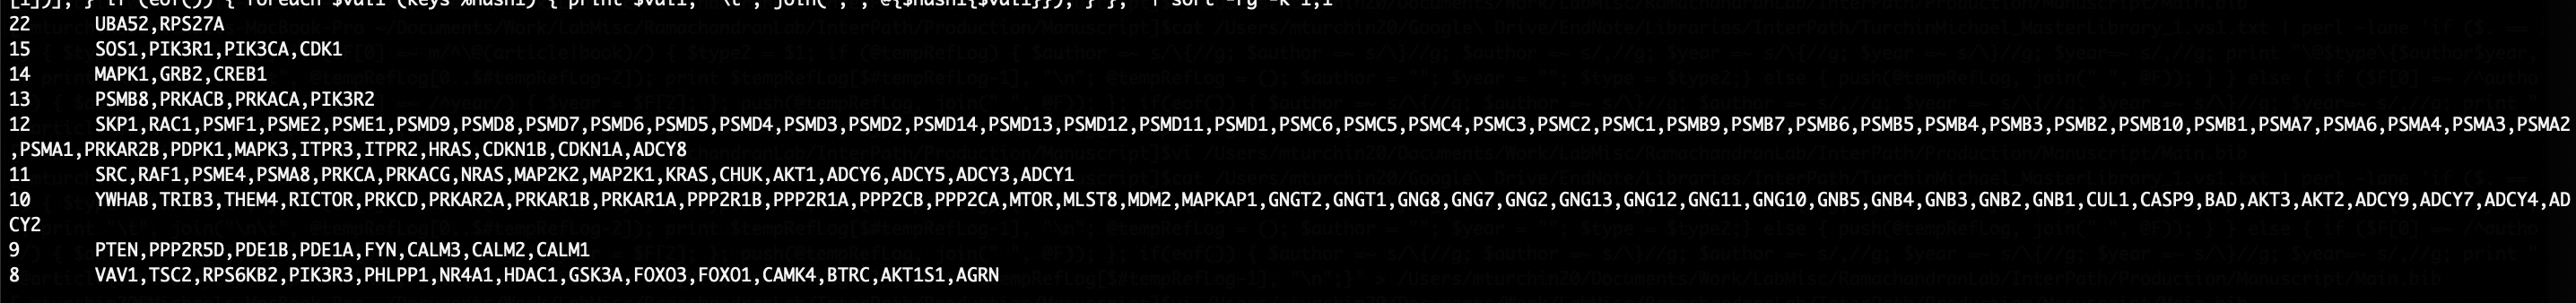
\includegraphics[scale=1]{Images/Supp/InterPath_Supp_Table_TopPathwayGeneCounts.png}
%\caption[TBD]{\textbf{Table of Most Present Genes in Significant MAPIT-R Pathways} \textcolor{red}{this will be a table}}
%\label{InterPath-Supp-Tables-GeneCounts}
%\end{figure}
%\end{landscape}
%\clearpage

\newcounter{CharNumber2}
\setcounter{CharNumber2}{1}
\renewcommand{\thetable}{\arabic{table}\alph{CharNumber2}}
\setlength{\footskip}{3cm}
\begin{landscape}
\begin{table}[ht]
\centering
\hspace*{-1.75cm}
\begin{tabular}{ccl}
  \hline
\textbf{Population} & \textbf{Gene Count} & \textbf{Genes} \\
  \hline
 \textbf{African} & & \\
 & 11 & MAPK3,MAPK1 \\
  & 10 & TNF \\
  &  9 & PRKCB,PLCB4,PLCB3,PLCB2,PLCB1,HRAS \\
  &  8 & RAF1,PRKCG,PRKCA,NRAS,MAP2K1,KRAS,HLA-G,HLA-E,HLA-DRB1,HLA-DRA,HLA-DQB1, \\
  & & HLA-DQA2,HLA-DQA1,HLA-DPB1,HLA-DPA1,HLA-DOB,HLA-DOA,HLA-DMB,HLA-DMA, \\
  & & HLA-C,HLA-B,HLA-A \\
  &  7 & PRKACG,PRKACB,PRKACA,MAP2K2,ITPR1,HLA-F,FAS,CD86,CD80,CD28,CACNA1C,BRAF \\
  &  6 & RAC2,RAC1,PRF1,PIK3R5,PIK3R3,PIK3R2,PIK3R1,PIK3CG,PIK3CD,PIK3CB,PIK3CA,ITPR3, \\ 
  & & ITPR2,IL2,IFNG,GNAQ,FASLG,CD40,CALML6,CALML5,CALML3,CALM3,CALM2,CALM1, \\
  & & CACNA1D,ADCY8,ADCY3,ADCY1 \\
  &  5 & SOS2,SOS1,ROCK2,ROCK1,RHOA,RAC3,PPP3R1,PPP3CC,PPP3CB,PPP3CA,PDGFRA,ITGB7, \\ 
  & & ITGB1,ITGA4,IL10,GZMB,EGFR,EGF,CXCR4,CHP2,CACNA1S,ADCY9,ADCY7,ADCY6, \\
  & & ADCY5,ADCY4,ADCY2,ACTG1,ACTB \\
  \\
  \textbf{Caribbean} & & \\
  & 6 & ITGB1 \\
  \\
  \textbf{Chinese} & & \\
  & 5 & HLA-DRB5,HLA-DRB1,HLA-DRA,HLA-DQB1,HLA-DQA2,HLA-DQA1,HLA-DPB1,HLA-DPA1, \\
  & & HLA-DOB,HLA-DOA,HLA-DMB,HLA-DMA \\
   \hline
\end{tabular}
\caption[TBD]{\textbf{Gene counts across MAPIT-R genome-wide significant KEGG pathways in height, per subset}. Caption continued at end of tables.}
\label{InterPath-Supp-Tables-AllPops-TopGeneCounts-KEGG-Height-a}
\end{table}
\clearpage
\addtocounter{table}{-1}
\addtocounter{CharNumber2}{1}

\begin{table}[ht]
\centering
\vspace*{-1.cm}
\hspace*{-1.75cm}
\begin{tabular}{ccl}
  \hline
\textbf{Population} & \textbf{Gene Count} & \textbf{Genes} \\
  \hline
  \textbf{African} & & \\
  & 18 & MAPK3,MAPK1 \\
  & 14 & PIK3CG,PIK3CD,PIK3CB,PIK3CA,HRAS \\
  & 13 & RAF1,PIK3R5,PIK3R3,PIK3R2,PIK3R1,NRAS,MAP2K1,KRAS \\
  & 12 & TNF,PRKCB,MAP2K2 \\
  & 11 & SOS2,SOS1 \\
  & 10 & PRKCG,PRKCA,HLA-DRB1,HLA-DRA,HLA-DQB1,HLA-DQA2,HLA-DQA1,HLA-DPB1,HLA-DPA1, \\
  & & HLA-DOB,HLA-DOA,HLA-DMB,HLA-DMA,GSK3B,GRB2,BRAF \\
  &  9 & TP53,RHOA,RAC1,PLCB4,PLCB3,PLCB2,PLCB1,ITGB1,CCND1,AKT3,AKT2,AKT1 \\
  &  8 & RAC2,PRKACG,PRKACB,PRKACA,PLCG1,ITGA4,IL10,IFNG,HLA-G,HLA-E,HLA-C,HLA-B, \\
  & & HLA-A,EP300,EGFR,CREBBP,CDC42,CD28 \\
  &  7 & PLCG2,IL4,IL2,HLA-F,FAS,EGF,CD86,CD80,CASP9,CAMK2G,CAMK2D,CAMK2B,CAMK2A, \\ 
  & & CALML6,CALML5,CALML3,CALM3,CALM2,CALM1,CACNA1C,ADCY8,ADCY3,ADCY1, \\
  & & ACTG1,ACTB \\
  &  6 & ROCK2,ROCK1,RELA,RAC3,PTK2,PRF1,PPP3R1,PPP3CC,PPP3CB,PPP3CA,PAK1,NFKBIA, \\ 
  & & NFKB1,LAMA2,ITGB7,ITGAV,ITGA6,ITGA3,ITGA2B,ITGA2,IL5,IKBKB,GNAQ,FASLG, \\
  & & CTNNB1,CHP2,CDK4,CD40,CACNA1D,ADCY9,ADCY7,ADCY6,ADCY5,ADCY4,ADCY2 \\
  &  5 & VAV3,VAV2,VAV1,TGFB1,TCF7L2,TCF7L1,TCF7,SHC4,SHC3,SHC2,SHC1,RB1,PTPN6,PTEN, \\ 
  & & PDGFRA,MYC,MDM2,MAPK9,LEF1,JUN,ITPR1,ITGB8,ITGB6,ITGB5,ITGB4,ITGB3,ITGB2, \\ 
  & & ITGA9,ITGA8,ITGA7,ITGA11,ITGA10,ITGA1,IGF1,GZMB,GNAI3,GNAI1,FYN,E2F3,E2F2,E2F1, \\ 
  & & DAG1,CYCS,CXCR4,CDKN1A,CDK6,CASP3,CACNA1S,BAD,ACTN4,ACTN3,ACTN2,ACTN1,ABL1 \\ 
  \\
  \textbf{Chinese} & & \\
  & 7 & HLA-DRB5,HLA-DRB1,HLA-DRA,HLA-DQB1,HLA-DQA2,HLA-DQA1,HLA-DPB1,HLA-DPA1, \\ 
  & & HLA-DOB,HLA-DOA,HLA-DMB,HLA-DMA \\
  &  6 & TNF \\
  &  5 & IFNG,HLA-G,HLA-F,HLA-E,HLA-C,HLA-B,HLA-A,CD86,CD80,CD28 \\
   \hline
\end{tabular}
\caption[TBD]{\textbf{Gene counts across MAPIT-R genome-wide significant KEGG pathways in BMI, per subset}}
\label{InterPath-Supp-Tables-AllPops-TopGeneCounts-KEGG-BMI-a}
\end{table}
\clearpage
\addtocounter{table}{-1}
\addtocounter{CharNumber2}{1}

\begin{table}[ht]
\centering
\vspace*{0cm}
\hspace*{-1.75cm}
\begin{tabular}{ccl}
  \hline
\textbf{Population} & \textbf{Gene Count} & \textbf{Genes} \\
  \hline
  \textbf{African} & & \\
   & 8 & MAPK1 \\
    & 7 & PIK3R2,PIK3R1,PIK3CA \\
    & 6 & SOS1,MAPK3,MAP2K2,MAP2K1,GRB2,CREB1,CDK1 \\
    & 5 & UBA52,RPS27A,RAF1,PRKCD,PRKACB,PPP2R5D,PPP2R1B,PPP2R1A,PPP2CB, \\
    & & PPP2CA,ITPR3,ITPR2,ITGB1,HRAS,GNGT2,GNGT1,GNG8,GNG7,GNG2,GNG13, \\ 
    & & GNG12,GNG11,GNG10,GNB5,GNB4,GNB3,GNB2,GNB1 \\
   \hline
\end{tabular}
\caption[TBD]{\textbf{Gene counts across MAPIT-R genome-wide significant REACTOME pathways in height, per subset}}
\label{InterPath-Supp-Tables-AllPops-TopGeneCounts-REACTOME-Height-a}
\end{table}
\clearpage
\addtocounter{table}{-1}
\addtocounter{CharNumber2}{1}

\begin{table}[ht]
\centering
\vspace*{-2cm}
\hspace*{-2cm}
\begin{tabular}{ccl}
  \hline
\textbf{Population} & \textbf{Gene Count} & \textbf{Genes} \\
  \hline
  \textbf{African} & & \\
  & 22 & UBA52,RPS27A \\
  & 15 & SOS1,PIK3R1,PIK3CA,CDK1 \\
  & 14 & MAPK1,GRB2,CREB1 \\
  & 13 & PSMB8,PRKACB,PRKACA,PIK3R2 \\
  & 12 & SKP1,RAC1,PSMF1,PSME2,PSME1,PSMD9,PSMD8,PSMD7,PSMD6,PSMD5,PSMD4,PSMD3, \\
  & & PSMD2,PSMD14,PSMD13,PSMD12,PSMD11,PSMD1,PSMC6,PSMC5,PSMC4,PSMC3,PSMC2, \\ 
  & & PSMC1,PSMB9,PSMB7,PSMB6,PSMB5,PSMB4,PSMB3,PSMB2,PSMB10,PSMB1,PSMA7, \\
  & & PSMA6,PSMA4,PSMA3,PSMA2,PSMA1,PRKAR2B,PDPK1,MAPK3,ITPR3,ITPR2,HRAS, \\
  & & CDKN1B,CDKN1A,ADCY8 \\
  & 11 & SRC,RAF1,PSME4,PSMA8,PRKCA,PRKACG,NRAS,MAP2K2,MAP2K1,KRAS,CHUK,AKT1, \\
  & & ADCY6,ADCY5,ADCY3,ADCY1 \\
  & 10 & YWHAB,TRIB3,THEM4,RICTOR,PRKCD,PRKAR2A,PRKAR1B,PRKAR1A,PPP2R1B, \\ 
  & & PPP2R1A,PPP2CB,PPP2CA,MTOR,MLST8,MDM2,MAPKAP1,GNGT2,GNGT1,GNG8,GNG7, \\
  & & GNG2,GNG13,GNG12,GNG11,GNG10,GNB5,GNB4,GNB3,GNB2,GNB1,CUL1,CASP9,BAD,AKT3, \\
  & & AKT2,ADCY9,ADCY7,ADCY4,ADCY2 \\
    & 9 & PTEN,PPP2R5D,PDE1B,PDE1A,FYN,CALM3,CALM2,CALM1 \\
    & 8 & VAV1,TSC2,RPS6KB2,PIK3R3,PHLPP1,NR4A1,HDAC1,GSK3A,FOXO3,FOXO1,CAMK4,BTRC, \\ 
    & & AKT1S1,AGRN \\
    & 7 & RPA3,RPA2,RPA1,RBX1,PRKCG,PRKCE,NCAN,CDK2 \\
    & 6 & TRIO,SHC1,SEH1L,SDC4,SDC3,SDC2,SDC1,RANBP2,PLCG1,PLCB3,PLCB2,PLCB1,PIK3CB, \\ 
    & & ORC5,ORC4,ORC3,ORC2,ORC1,NUP85,NUP43,NUP37,NUP133,NUP107,MYC,MCM8,MCM7, \\
    & & MCM6,MCM5,MCM4,MCM3,MCM2,LCK,KALRN,HSPG2,GPC6,GPC5,GPC2,GPC1,GNAS, \\ 
    & & GNAI2,GNAI1,E2F3,E2F1,CDC6,CDC42,ADAM17 \\  
    & 5 & YES1,WEE1,VCAN,STAT5B,STAT5A,STAT3,STAG1,SMC3,SAA1,RELA,RASGRF2,RASGRF1, \\
    & & RAD21,PTPN6,PSEN2,PSEN1,PRIM2,PRIM1,POLE2,POLE,POLA2,PLA2G4A,PAK2,NCSTN, \\
    & & MNAT1,MCM10,MAPK8,MAPK14,ITGB3BP,IKBKB,HIST4H4,HIST2H2AA3,HIST1H4L, \\
    & & HIST1H4K,HIST1H4J,HIST1H4H,HIST1H4F,HIST1H4E,HIST1H4D,HIST1H4C,HIST1H4B, \\
    & & HIST1H4A,HIST1H2BO,HIST1H2BN,HIST1H2BM,HIST1H2BL,HIST1H2BK,HIST1H2BJ,HIST1H2BI, \\
    & & HIST1H2BH,HIST1H2BG,HIST1H2BF,HIST1H2BE,HIST1H2BD,HIST1H2BC,HIST1H2BB, \\
    & & HIST1H2AJ,HIST1H2AE,HIST1H2AD,HIST1H2AC,HIST1H2AB,HEXB,HEXA,HDAC2,H2AFZ, \\
    & & GXYLT2,GXYLT1,GRP,GCGR,FFAR1,EP300,E2F2,DCN,DBF4,CSPG4,CRK,CREBBP,CHRM3, \\
    & & CDT1,CDK7,CDC7,CDC45,CCNH,BCAN,B4GALT7,B3GAT2,B3GAT1,B3GALT6,ATR,APP, \\ 
    & & APH1B,APH1A,AP2S1,AP2M1,AP2B1,AP2A2,AP2A1 \\
   \hline
\end{tabular}
\caption[TBD]{\textbf{Gene counts across MAPIT-R genome-wide significant REACTOME pathways in BMI, per subset}}
\label{InterPath-Supp-Tables-AllPops-TopGeneCounts-REACTOME-BMI-a}
\end{table}
\clearpage
\addtocounter{table}{-1}
\addtocounter{CharNumber2}{1}
\end{landscape}
\renewcommand{\thetable}{\arabic{table}}
\setlength{\footskip}{1cm}

\begin{table} [t!]
  \caption{\textbf{Gene counts across MAPIT-R genome-wide significant pathways, per subset}. The tables show the lists of genes that appear most frequently across the pathways that were MAPIT-R genome-wide significant in the following phenotype and pathway database combinations: (a) KEGG height, (b) KEGG BMI, (c) REACTOME height, and (d) REACTOME BMI. The first columns list the UKB subsets, the second columns list the number of times the given genes appeared in the set of genome-wide significant pathways for that subset, pathway database, and phenotype combination, and the third columns list the actual gene names for each of these numbers of gene counts.}
\label{InterPath-Supp-Tables-AllPops-TopGeneCounts-Caption}
\end{table}
\clearpage

\setlength{\footskip}{2cm}
\begin{table}[ht]
\centering
\begin{tabular}{ccccc}
  \hline
  \textbf{Database} & \textbf{Gene} & \textbf{No Restriction} & \textbf{Restricted} & \textbf{-$\log_{10}$($p$-Value)} \\
  & & \textbf{$p$-Value} & \textbf{$p$-Value} & \textbf{Difference} \\
  \hline
  \textbf{KEGG:} & & & & \\
  & CDKN2A & 1.248E-01 & 7.974E-03 & 1.194 \\
  & CCNB2 & 2.795E-01 & 1.876E-02 & 1.173 \\
  & CCNB1 & 2.795E-01 & 1.876E-02 & 1.173 \\
  & PTEN & 5.340E-02 & 4.186E-03 & 1.106 \\
  & GADD45G & 6.710E-02 & 6.559E-03 & 1.010 \\
  & GADD45B & 6.710E-02 & 6.559E-03 & 1.010 \\
  & GADD45A & 6.710E-02 & 6.559E-03 & 1.010 \\
  & CHEK2 & 6.710E-02 & 6.559E-03 & 1.010 \\
  & CHEK1 & 6.710E-02 & 6.559E-03 & 1.010 \\
  & ATR & 6.710E-02 & 6.559E-03 & 1.010 \\
  \\
  \textbf{REACTOME:} & & & & \\ 
  & SMC3 & 1.456E-05 & 5.589E-09 & 3.416 \\
  & PSM* & 5.304E-04 & 4.464E-06 & 2.075 \\
  & (Cluster) & & & \\ 
  & FBXW11 & 7.902E-02 & 1.956E-03 & 1.606 \\
  & NFKBIE & 2.702E-02 & 1.956E-03 & 1.140 \\
  & PRKCB & 2.204E-01 & 1.797E-02 & 1.089 \\
  & MALT1 & 7.902E-02 & 1.109E-02 & 0.853 \\
  & LOC646626 & 7.902E-02 & 1.109E-02 & 0.853 \\
  & CARD11 & 7.902E-02 & 1.109E-02 & 0.8.53 \\
  & BCL10 & 7.902E-02 & 1.109E-02 & 0.8.53 \\
  & ATR & 8.004E-03 & 1.261E-03 & 0.8.02 \\
   \hline
\end{tabular}
\caption[TBD]{\textbf{Size restricted examples of gene count hypergeometric enrichment tests}. The table shows the top examples of genes that became more significant in the hypergeometric enrichment analyses after the size restriction step in both pathway databases. Results are only shown for BMI since the majority of genome-wide significant pathways in height were lost from the size restriction step alone. The first column lists the pathway database, the second column lists the genes, the third column lists the original, unrestricted hypergeometric enrichment $p$-value, the fourth column lists the new, size-restricted hypergeometric enrichment $p$-value, and the fifth column lists the -$\log_{10}$ $p$-value difference between the third and fourth column. The top 10 genes sorted by the fifth column are shown for each database. For a plot of results from every gene analyzed in both databases, see Supplementary Figure \ref{InterPath-Supp-Figure-Hypergeometric-RestrictedComps-African-BMI}). Note that a single entry in the REACTOME results is included to represent the PSM* gene family cluster to preserve space.}
\label{InterPath-Supp-Table-Hypergeometric-RestrictedComps-African-BMI-TopExamples}
\end{table}
\clearpage
\setlength{\footskip}{1cm}

\begin{landscape}
\begin{table}[ht]
\centering
\hspace*{-1.5cm}
\begin{tabular}{ccccccc}
  \hline
  \textbf{Gene} & \textbf{Pathway SNP} & \textbf{Gene Count in} & \textbf{Total Count of} & \textbf{Gene Count in} & \textbf{Total Count of} & \textbf{Hypergeometric} \\
   & \textbf{Count Limit} & \textbf{Top Pathways} & \textbf{Top Pathways} & \textbf{All Pathways} & \textbf{All Pathways} & \textbf{$p$-Value} \\
  \hline
 \textbf{UBA52} & & & & & & \\
 & No Limit & 22 & 65 & 106 & 658 & 1.537E-4 \\
 & $<=$ 1000 SNPs & 10 & 26 & 84 & 577 & 1.855E-3 \\
\\
 \textbf{PSM*} & & & & & & \\
 & No Limit & 12 & 65 & 44 & 658 & 5.304E-4 \\
 & $<=$ 1000 SNPs & 9 & 26 & 34 & 577 & 4.464E-6 \\
   \hline
\end{tabular}
\caption[TBD]{\textbf{MAPIT-R Genome-Wide Significant Pathway Gene Counts: Hypergeometric Enrichment Examples}. Caption continued on next page.}
\label{InterPath-Supp-Tables-AllPops-TopGeneCount-HypergeometricTests}
\end{table}
\end{landscape}
\clearpage

\addtocounter{table}{-1}
\begin{table} [t!]
  \caption{\textbf{PSM* and UBA52 gene count enrichment test examples, size restriction and no restriction}. The table shows examples and results of running the hypergeometric test for enrichment on two different genes in two different study designs. In all cases a gene is tested for being significantly more frequent among the set of MAPIT-R genome-wide significant pathways than among the background distribution of pathways in the original database. Two study designs were employed for these tests, either (a) using all pathways present in the given databases or (b) using only pathways that contained less than or equal to 1,000 SNPs. The first column lists the gene or gene family being tested. The second column lists which of the two aforementioned study designs was used. Columns three through six list the different count values used in the hypergeometric test: the third column lists the number of times a gene is present among the genome-wide significant list of pathways, the fourth column lists the total number of pathways that were genome-wide significant, the fifth column lists the number of times a gene is present among all the pathways in the given database, and the sixth column lists the total number of pathways in the given database. The seventh column is the hypergeometric $p$-value associated with columns three through six. Note that the vast majority of proteasome genes included in our analysis had the same number of gene counts across each hypergeometric category, hence why \textbf{PSM*} was used to represent them as a whole.}
\label{InterPath-Supp-Tables-AllPops-TopGeneCount-HypergeometricTests-Caption}
\end{table}
\clearpage

\begin{landscape}
\setlength{\footskip}{2cm}
\begin{table}[ht]
\centering
\begin{tabular}{lrrr}
  \hline
\textbf{Pathway} & \textbf{Genes} & \textbf{SNPs} & \textbf{$p$-Value} \\ 
  \hline
REACTOME\_M\_G1\_TRANSITION & 73 & 458 & 3.191E-06 \\ 
  REACTOME\_CELL\_CYCLE\_CHECKPOINTS & 105 & 670 & 5.781E-06 \\ 
  REACTOME\_HOST\_INTERACTIONS\_OF\_HIV\_FACTORS & 112 & 963 & 7.521E-06 \\ 
  REACTOME\_DOWNSTREAM\_SIGNALING\_EVENTS\_OF\_ & & & \\ 
  \qquad B\_CELL\_RECEPTOR\_BCR & 89 & 745 & 1.195E-05 \\
  REACTOME\_REGULATION\_OF\_APOPTOSIS & 52 & 564 & 1.218E-05 \\ 
  REACTOME\_MITOTIC\_G1\_G1\_S\_PHASES & 121 & 747 & 1.453E-05 \\ 
  REACTOME\_ACTIVATION\_OF\_NF\_KAPPAB\_IN\_B\_CELLS & 59 & 465 & 1.861E-05 \\ 
  REACTOME\_ASSEMBLY\_OF\_THE\_PRE\_REPLICATIVE\_COMPLEX & 60 & 331 & 3.293E-05 \\ 
  REACTOME\_ANTIGEN\_PROCESSING\_CROSS\_PRESENTATION & 68 & 850 & 3.956E-05 \\ 
   \hline
\end{tabular}
  \caption{\textbf{Size-restricted pathways that contain the PSM* cluster of genes}. Caption continued on next page.}
\label{InterPath-Supp-Tables-AllPops-TopGeneCount-SizeRestricted-Proteasome}
\end{table}
\clearpage
\end{landscape}
\setlength{\footskip}{1cm}

\addtocounter{table}{-1}
\begin{table} [t!]
  \caption{\textbf{Size-restricted pathways that contain the PSM* cluster of genes}. The table shows the MAPIT-R genome-wide significant REACTOME pathways for BMI in the African subset that both have SNP sizes less than 1,000 and also contain the set of proteasome genes being investigated (\textit{PSMA}*, \textit{PSMB}*, \textit{PSMC}*, \textit{PSMD}*, and \textit{PSME*}). The first column shows the REACTOME pathway names, the second column shows the number of genes that were included in the MAPIT-R analysis, the third column show the number of SNPs that were included in the MAPIT-R analysis, and the fourth column shows the MAPIT-R $p$-value.}
\label{InterPath-Supp-Tables-AllPops-TopGeneCount-SizeRestricted-Proteasome-Caption}
\end{table}
\clearpage

%\begin{figure}[htbp]
%\centering
%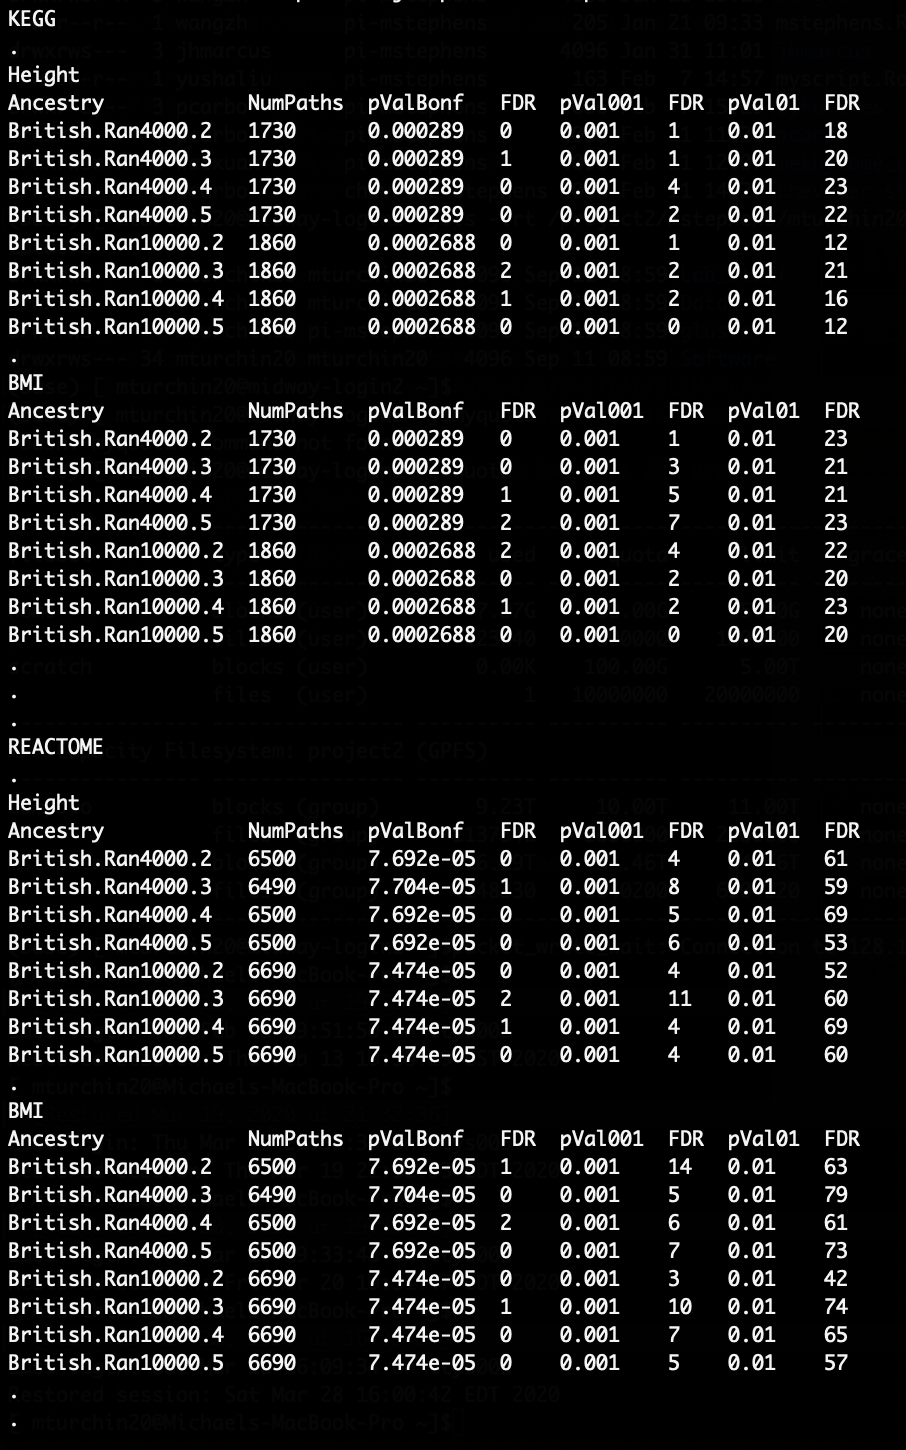
\includegraphics[scale=1.5]{Images/Supp/InterPath_Supp_Figure_FDRs_BritReps_vs1.png}
%\caption[TBD]{\textbf{TBD}. }
%\label{InterPath-Supp-Figure-BritReps-FDRs}
%\end{figure}
%\clearpage

\setlength{\footskip}{4cm}
\begin{landscape}
\begin{table}[ht]
\vspace*{-1.25cm}
\centering
\hspace*{-3.25cm}
\begin{tabular}{ccccccccccc}
  \hline
\textbf{Population} & \textbf{Pathway} & \textbf{Bonferroni} & \textbf{Bonferroni} & \textbf{Bonferroni} & \textbf{0.001} & \textbf{0.001} & \textbf{0.001} & \textbf{0.01} & \textbf{0.01} & \textbf{0.01} \\
 & \textbf{Counts} & \textbf{Threshold} & \textbf{Counts} & \textbf{FDR} & \textbf{Threshold} & \textbf{Counts} & \textbf{FDR} & \textbf{Threshold} & \textbf{Counts} & \textbf{FDR} \\ 
  \hline
\textbf{KEGG Height:} & & & & & & & & & \\
British.Ran4000 & 1730 & 2.890E-04 & 0 & 0.000 & 0.001 & 0 & 0.000 & 0.010 & 13 & 0.751 \\
  British.Ran4000.2 & 1730 & 2.890E-04 & 0 & 0.000 & 0.001 & 1 & 0.058 & 0.010 & 18 & 1.040 \\
  British.Ran4000.3 & 1730 & 2.890E-04 & 1 & 0.058 & 0.001 & 1 & 0.058 & 0.010 & 20 & 1.156 \\
  British.Ran4000.4 & 1730 & 2.890E-04 & 0 & 0.000 & 0.001 & 4 & 0.231 & 0.010 & 23 & 1.329 \\
  British.Ran4000.5 & 1730 & 2.890E-04 & 0 & 0.000 & 0.001 & 2 & 0.116 & 0.010 & 22 & 1.272 \\
  British.Ran10000.1 & 1860 & 2.688E-04 & 0 & 0.000 & 0.001 & 1 & 0.054 & 0.010 & 26 & 1.398 \\
  British.Ran10000.2 & 1860 & 2.688E-04 & 0 & 0.000 & 0.001 & 1 & 0.054 & 0.010 & 12 & 0.645 \\
  British.Ran10000.3 & 1860 & 2.688E-04 & 2 & 0.108 & 0.001 & 2 & 0.108 & 0.010 & 21 & 1.129 \\
  British.Ran10000.4 & 1860 & 2.688E-04 & 1 & 0.054 & 0.001 & 2 & 0.108 & 0.010 & 16 & 0.860 \\
  British.Ran10000.5 & 1860 & 2.688E-04 & 0 & 0.000 & 0.001 & 0 & 0.000 & 0.010 & 12 & 0.645 \\
  \\
  \textbf{KEGG BMI:} & & & & & & & & & \\
British.Ran4000 & 1730 & 2.890E-04 & 1 & 0.058 & 0.001 & 2 & 0.116 & 0.010 & 14 & 0.809 \\
  British.Ran4000.2 & 1730 & 2.890E-04 & 0 & 0.000 & 0.001 & 1 & 0.058 & 0.010 & 23 & 1.329 \\
  British.Ran4000.3 & 1730 & 2.890E-04 & 0 & 0.000 & 0.001 & 3 & 0.173 & 0.010 & 21 & 1.214 \\
  British.Ran4000.4 & 1730 & 2.890E-04 & 1 & 0.058 & 0.001 & 5 & 0.289 & 0.010 & 21 & 1.214 \\
  British.Ran4000.5 & 1730 & 2.890E-04 & 2 & 0.116 & 0.001 & 7 & 0.405 & 0.010 & 23 & 1.329 \\
  British.Ran10000.1 & 1860 & 2.688E-04 & 0 & 0.000 & 0.001 & 1 & 0.054 & 0.010 & 25 & 1.344 \\
  British.Ran10000.2 & 1860 & 2.688E-04 & 2 & 0.108 & 0.001 & 4 & 0.215 & 0.010 & 22 & 1.183 \\
  British.Ran10000.3 & 1860 & 2.688E-04 & 0 & 0.000 & 0.001 & 2 & 0.108 & 0.010 & 20 & 1.075 \\
  British.Ran10000.4 & 1860 & 2.688E-04 & 1 & 0.054 & 0.001 & 2 & 0.108 & 0.010 & 23 & 1.237 \\
  British.Ran10000.5 & 1860 & 2.688E-04 & 0 & 0.000 & 0.001 & 0 & 0.000 & 0.010 & 20 & 1.075 \\
   \hline
\end{tabular}
\caption[TBD]{\textbf{MAPIT-R false discovery rates at different significance thresholds, per British replicate}. Caption continued at end of tables.}
\label{InterPath-Supp-Tables-BritReps-FDRs-pt1}
\end{table}
\end{landscape}
\clearpage
\setlength{\footskip}{1cm}
\addtocounter{table}{-1}

\setlength{\footskip}{4cm}
\renewcommand{\thetable}{\arabic{table}}
\begin{landscape}
\begin{table}[ht]
\vspace*{-1.25cm}
\centering
\hspace*{-3.5cm}
\begin{tabular}{ccccccccccc}
  \hline
\textbf{Population} & \textbf{Pathway} & \textbf{Bonferroni} & \textbf{Bonferroni} & \textbf{Bonferroni} & \textbf{0.001} & \textbf{0.001} & \textbf{0.001} & \textbf{0.01} & \textbf{0.01} & \textbf{0.01} \\
 & \textbf{Counts} & \textbf{Threshold} & \textbf{Counts} & \textbf{FDR} & \textbf{Threshold} & \textbf{Counts} & \textbf{FDR} & \textbf{Threshold} & \textbf{Counts} & \textbf{FDR} \\ 
  \hline
  \textbf{REACTOME Height:} & & & & & & & & & \\
British.Ran4000 & 6500 & 7.692E-05 & 0 & 0.000 & 0.001 & 9 & 0.138 & 0.010 & 69 & 1.062 \\
  British.Ran4000.2 & 6500 & 7.692E-05 & 0 & 0.000 & 0.001 & 4 & 0.062 & 0.010 & 61 & 0.938 \\
  British.Ran4000.3 & 6490 & 7.704E-05 & 1 & 0.015 & 0.001 & 8 & 0.123 & 0.010 & 59 & 0.909 \\
  British.Ran4000.4 & 6500 & 7.692E-05 & 0 & 0.000 & 0.001 & 5 & 0.077 & 0.010 & 69 & 1.062 \\
  British.Ran4000.5 & 6500 & 7.692E-05 & 0 & 0.000 & 0.001 & 6 & 0.092 & 0.010 & 53 & 0.815 \\
   British.Ran10000.1 & 6690 & 7.474E-05 & 0 & 0.000 & 0.001 & 4 & 0.060 & 0.010 & 55 & 0.822 \\
  British.Ran10000.2 & 6690 & 7.474E-05 & 0 & 0.000 & 0.001 & 4 & 0.060 & 0.010 & 52 & 0.777 \\
  British.Ran10000.3 & 6690 & 7.474E-05 & 2 & 0.030 & 0.001 & 11 & 0.164 & 0.010 & 60 & 0.897 \\
  British.Ran10000.4 & 6690 & 7.474E-05 & 1 & 0.015 & 0.001 & 4 & 0.060 & 0.010 & 69 & 1.031 \\
  British.Ran10000.5 & 6690 & 7.474E-05 & 0 & 0.000 & 0.001 & 4 & 0.060 & 0.010 & 60 & 0.897 \\

  \\
  \textbf{REACTOME BMI:} & & & & & & & & & \\
British.Ran4000 & 6490 & 7.704E-05 & 1 & 0.015 & 0.001 & 4 & 0.062 & 0.010 & 52 & 0.801 \\
  British.Ran4000.2 & 6500 & 7.692E-05 & 1 & 0.015 & 0.001 & 14 & 0.215 & 0.010 & 63 & 0.969 \\
  British.Ran4000.3 & 6490 & 7.704E-05 & 0 & 0.000 & 0.001 & 5 & 0.077 & 0.010 & 79 & 1.217 \\
  British.Ran4000.4 & 6500 & 7.692E-05 & 2 & 0.031 & 0.001 & 6 & 0.092 & 0.010 & 61 & 0.938 \\
  British.Ran4000.5 & 6500 & 7.692E-05 & 0 & 0.000 & 0.001 & 7 & 0.108 & 0.010 & 73 & 1.123 \\
  British.Ran10000.1 & 6690 & 7.474E-05 & 2 & 0.030 & 0.001 & 10 & 0.149 & 0.010 & 73 & 1.091 \\
  British.Ran10000.2 & 6690 & 7.474E-05 & 0 & 0.000 & 0.001 & 3 & 0.045 & 0.010 & 42 & 0.628 \\
  British.Ran10000.3 & 6690 & 7.474E-05 & 1 & 0.015 & 0.001 & 10 & 0.149 & 0.010 & 74 & 1.106 \\
  British.Ran10000.4 & 6690 & 7.474E-05 & 0 & 0.000 & 0.001 & 7 & 0.105 & 0.010 & 65 & 0.972 \\
  British.Ran10000.5 & 6690 & 7.474E-05 & 0 & 0.000 & 0.001 & 5 & 0.075 & 0.010 & 57 & 0.852 \\
   \hline
\end{tabular}
\caption[TBD]{\textbf{MAPIT-R false discovery rates at different significance thresholds, per British replicate}. Continued.}
\label{InterPath-Supp-Tables-BritReps-FDRs-pt2}
\end{table}
\end{landscape}
\clearpage
\setlength{\footskip}{1cm}

\addtocounter{table}{-1}
\begin{table} [t!]
  \caption{\textbf{MAPIT-R false discovery rates at different significance thresholds, per British replicate}. The tables show for various significance thresholds the false discovery rates observed from MAPIT-R when run on ten rounds of phenotype permutations for each British replicate subsample and pathway database. The first column lists the pathway database, phenotype, and British replicate subsample combinations. The second column lists the total number of pathways that were tested across each of the ten phenotype permutations. The third column shows the $p$-value threshold associated with using the Bonferroni method of correction, also known as the `genome-wide significant' threshold. The fourth column shows the number of pathways across all ten phenotype permutation rounds that crossed this Bonferroni threshold. The fifth column shows the associated FDR associated with the fourth column. And the remaining six columns show the same setup as columns three to five but with a $p$-value threshold of either 0.001 or 0.01.}
\label{InterPath-Supp-Tables-BritReps-FDRs-Caption}
\end{table}
\clearpage

\begingroup
\bibliographystyle{apalike}
\setstretch{1.0}
\bibliography{Main}
\endgroup


\iffalse

SCRAP

Additionally, it is unlikely that, even if such an ascertainment bias existed, it could continually be directionality consistent across pathways that span the genome. If this were an approach that aggregated single SNP tests, then directionality would not be an issue and one might become concerned about continually incorporating a persistent signal from ascertainment bias; however, because this is a joint test on multiple SNPs as once, it is far less likely that differences between genotype chip SNP distributions and non-European population SNP distributions tracts in exactly the same direction across the entire genome.




\subsection{Genome Level Epistasis}\label{InterPath-Results-GenomeEpistasis}

To investigate epistasis in multiple human populations, we first extracted a variety of human ancestries from the UKB (see Online Methods). We collected a total of 8 UKB subsets with an average sample size of XXXX among the non-European populations (Supplementary Table 1), including African, Indian, Chinese, and Pakistani subsets. To maximize our sample sizes per subset, we focused on height and body mass index (BMI) as our complex traits of interest. 

The first approach we took to investigate epistasis was to look at genome-wide estimates of phenotypic PVE. Specifically, we setup a linear mixed model that incorporated both additive and epistatic interactions, and fit each of these variance components using GEMMA \citep{Zhou2012} (see Online Methods and Supplementary Note for details). Calculating these variance component PVEs for height and BMI in each of our populations, we indeed find differences across each human ancestry (Table 1).

\begin{figure}[ht]
\centering
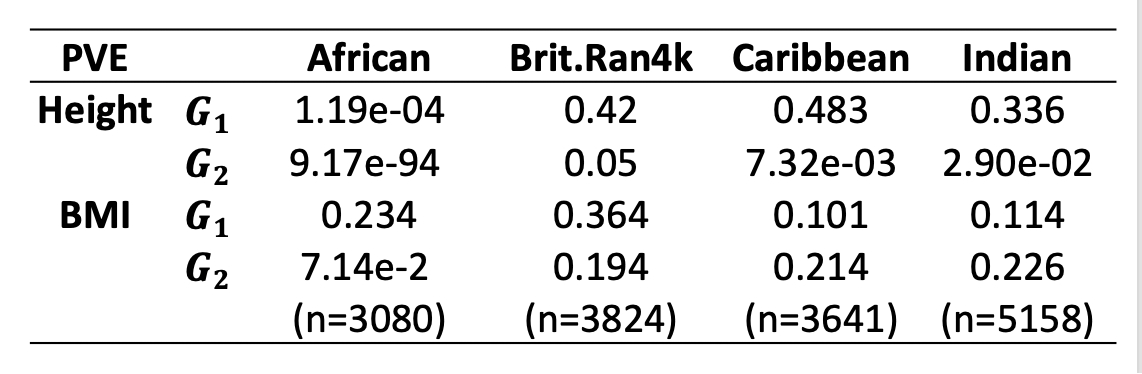
\includegraphics[scale=1]{Images/Table1_Placeholder.png}
\caption[TBD]{\textbf{TBD}. \\ this will be a table not a figure.}
\label{IntrePath-Main-Table-GEMMA}
\end{figure}

In height, we do not see anything immediately new. For the additive effects $G_1$ we mainly calculate PVEs across each population within our range of expectation (between XX and XX (citation)). Additionally, we do not currently see much evidence for second-order effects $G_2$. However, looking at BMI we see a different result. Across all populations we see non-trivial PVEs for $G_2$, ranging from XX to XX. We also see larger values in multiple non-European populations. In particular we see a particularly strong result in XXX. This might be beginning evidence that indeed, non-European populations have more potential for picking up signals of higher-order interactions in the genome.   




Information idea about creating random 'pathways' that have either the same number of genes or SNPs to show that it has to be the *right* collection of information/materials to get the same amount of significance

\subsubsection{Power Gained from Proper Pathway Definitions}

Running a GWAS of height and BMI on each of our population subsets with PLINK, we find only one genome-wide significant hit (Figure \ref{InterPath-Main-Figure-GWAS-Height} \& Supplementary Figure \ref{InterPath-Supp-Figure-GWAS-BMI}). And further similarly to before, we also find a handful of marginally significant variants. More interestingly however, we now ask how similar the MAPIT and GWAS results are. And indeed, comparing the two sets of genome-wide analyzes, we see a wide range of different genetic architecture patterns being represented (Figure \ref{InterPath-Main-Figure-MAPITvsGWAS-AfrHght} \& Supplementary Figure \ref{InterPath-Supp-Figure-MAPITvsGWAS}). Focusing on the African subset and height, we find 49 SNPs that are only marginally significant in MAPIT, 50 SNPs that are only marginally significant in the GWAS, and 0 SNPs that are marginally significant in both tests. Despite the lack of power to identify genome-wide significant results, we still see a strong representation of the partition of additive and epistatic effects in our results. 

\begin{figure}[htbp]
\centering
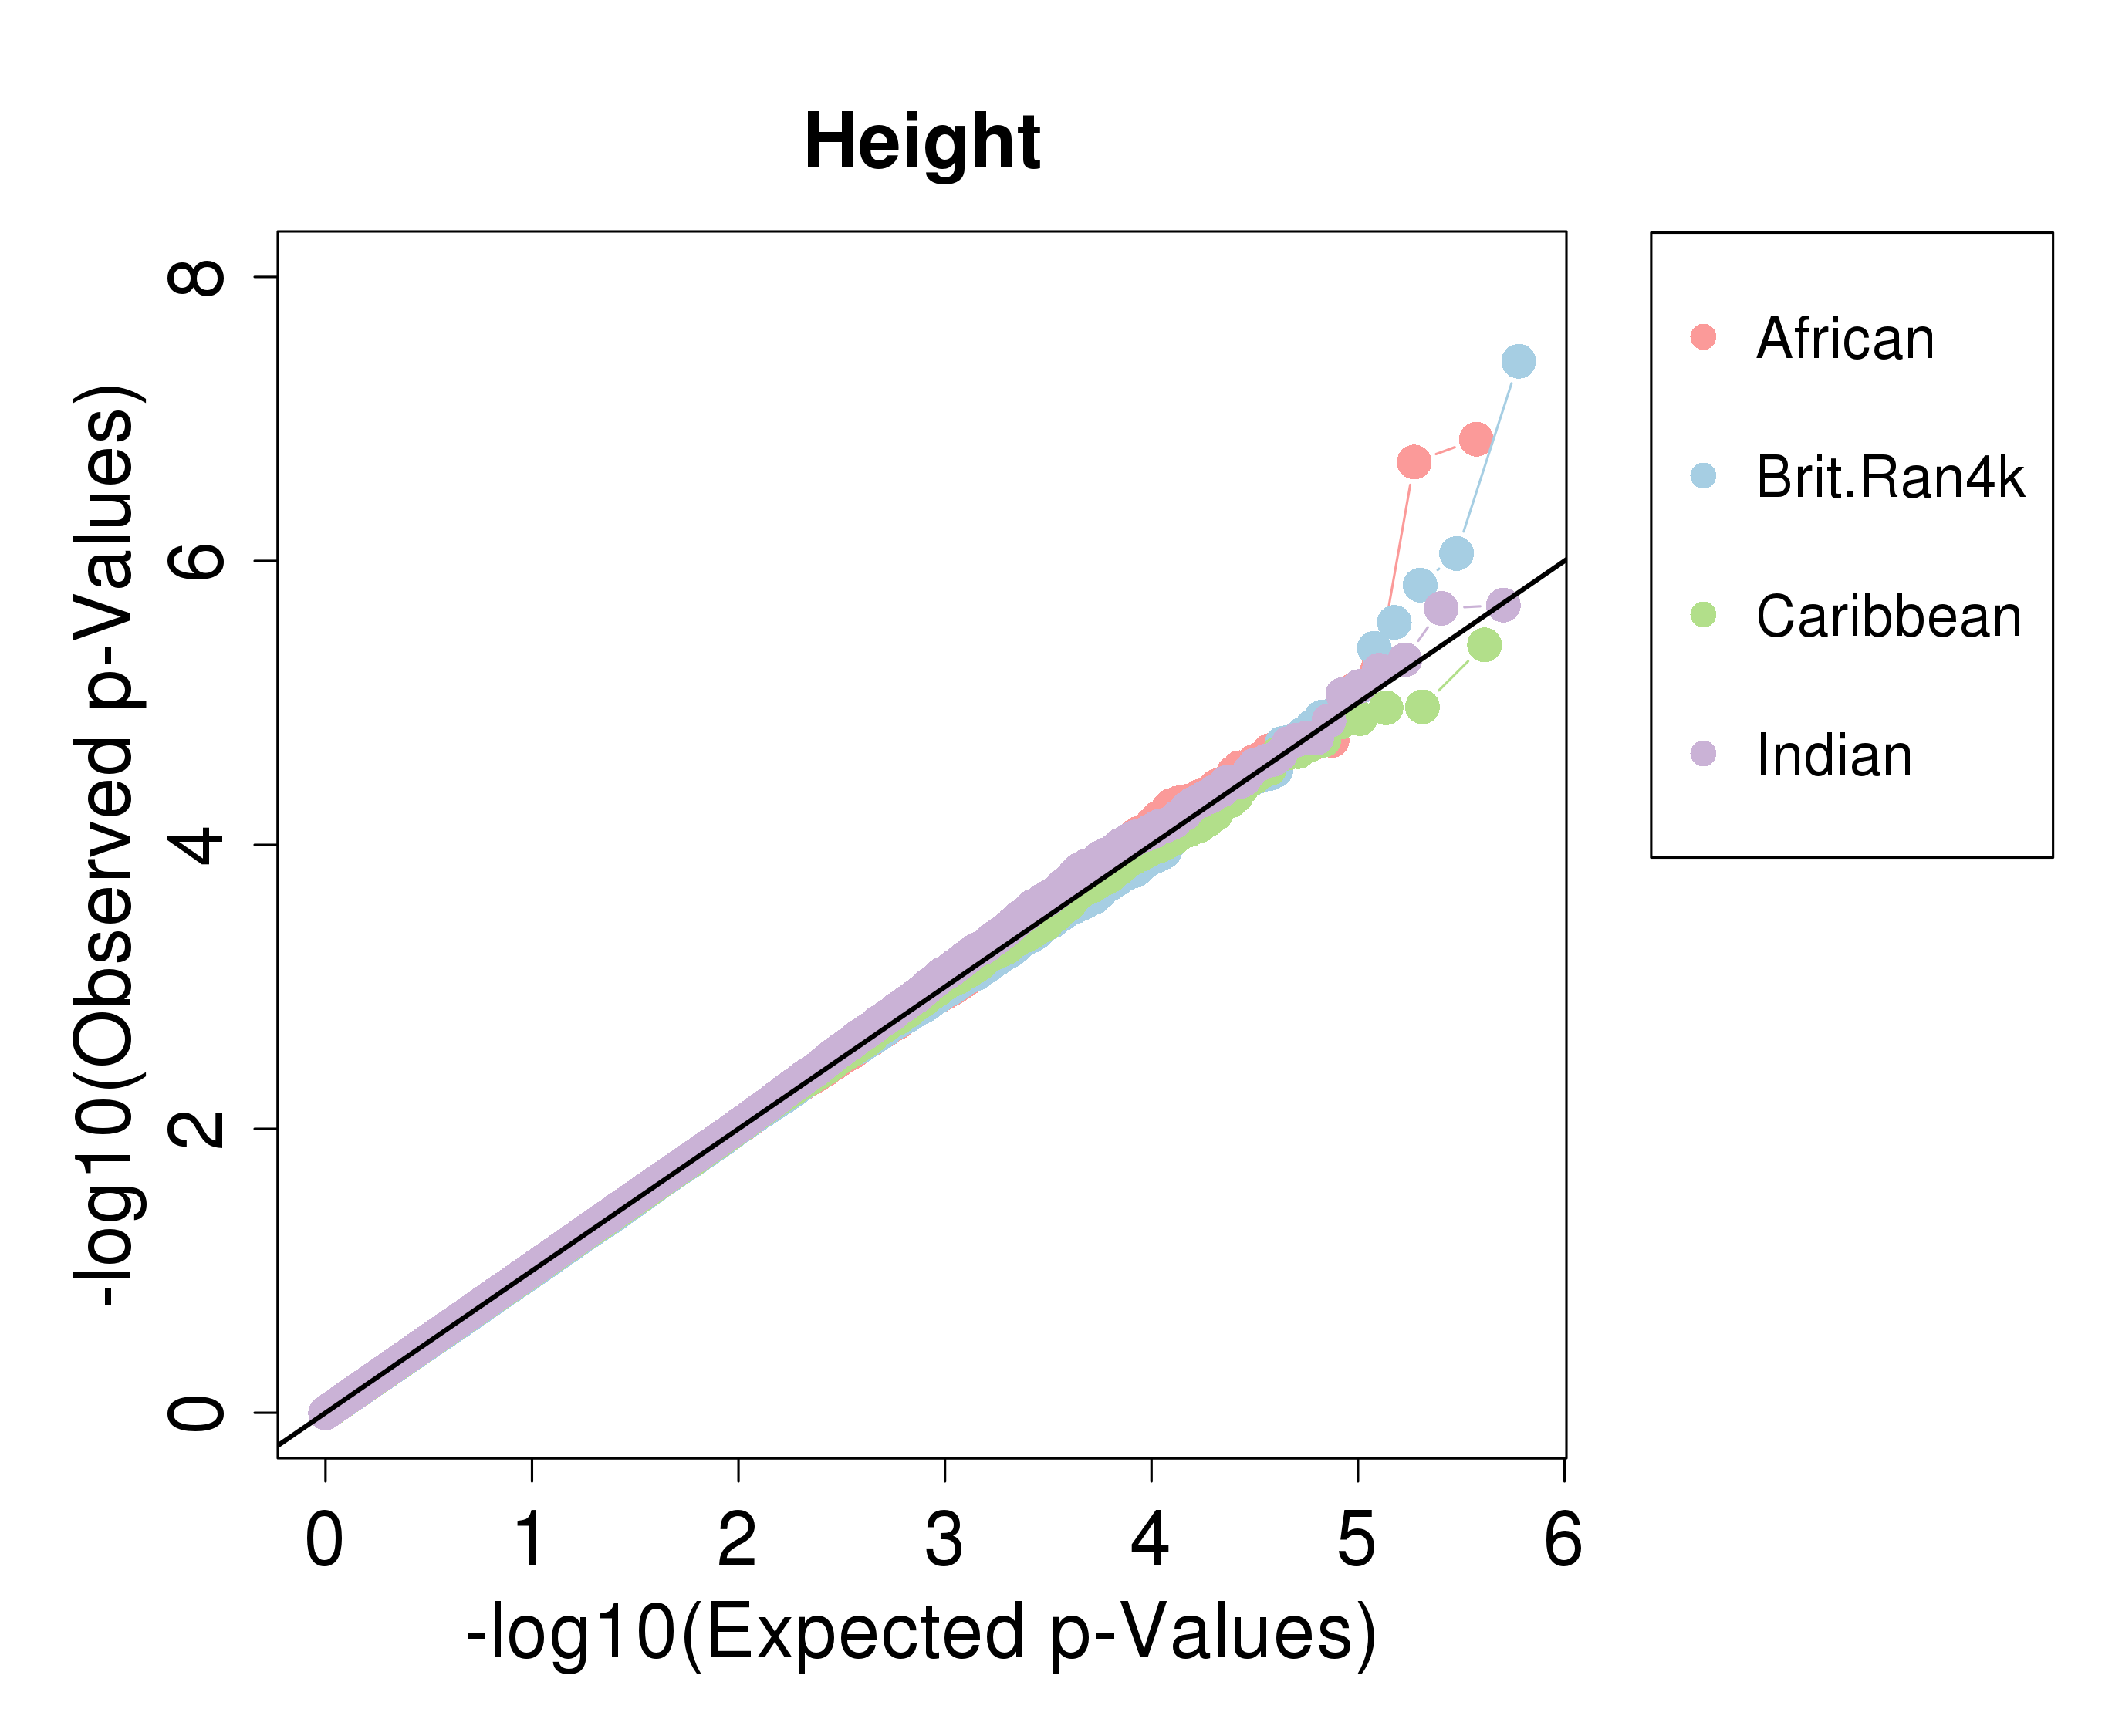
\includegraphics[scale=.35]{Images/Main/InterPath_Main_Figure_GWAS_vs2_Height.png}
\caption[TBD]{\textbf{GWAS Results QQ-Plots}.}
\label{InterPath-Main-Figure-GWAS-Height}
\end{figure}

\begin{figure}[htbp]
\centering
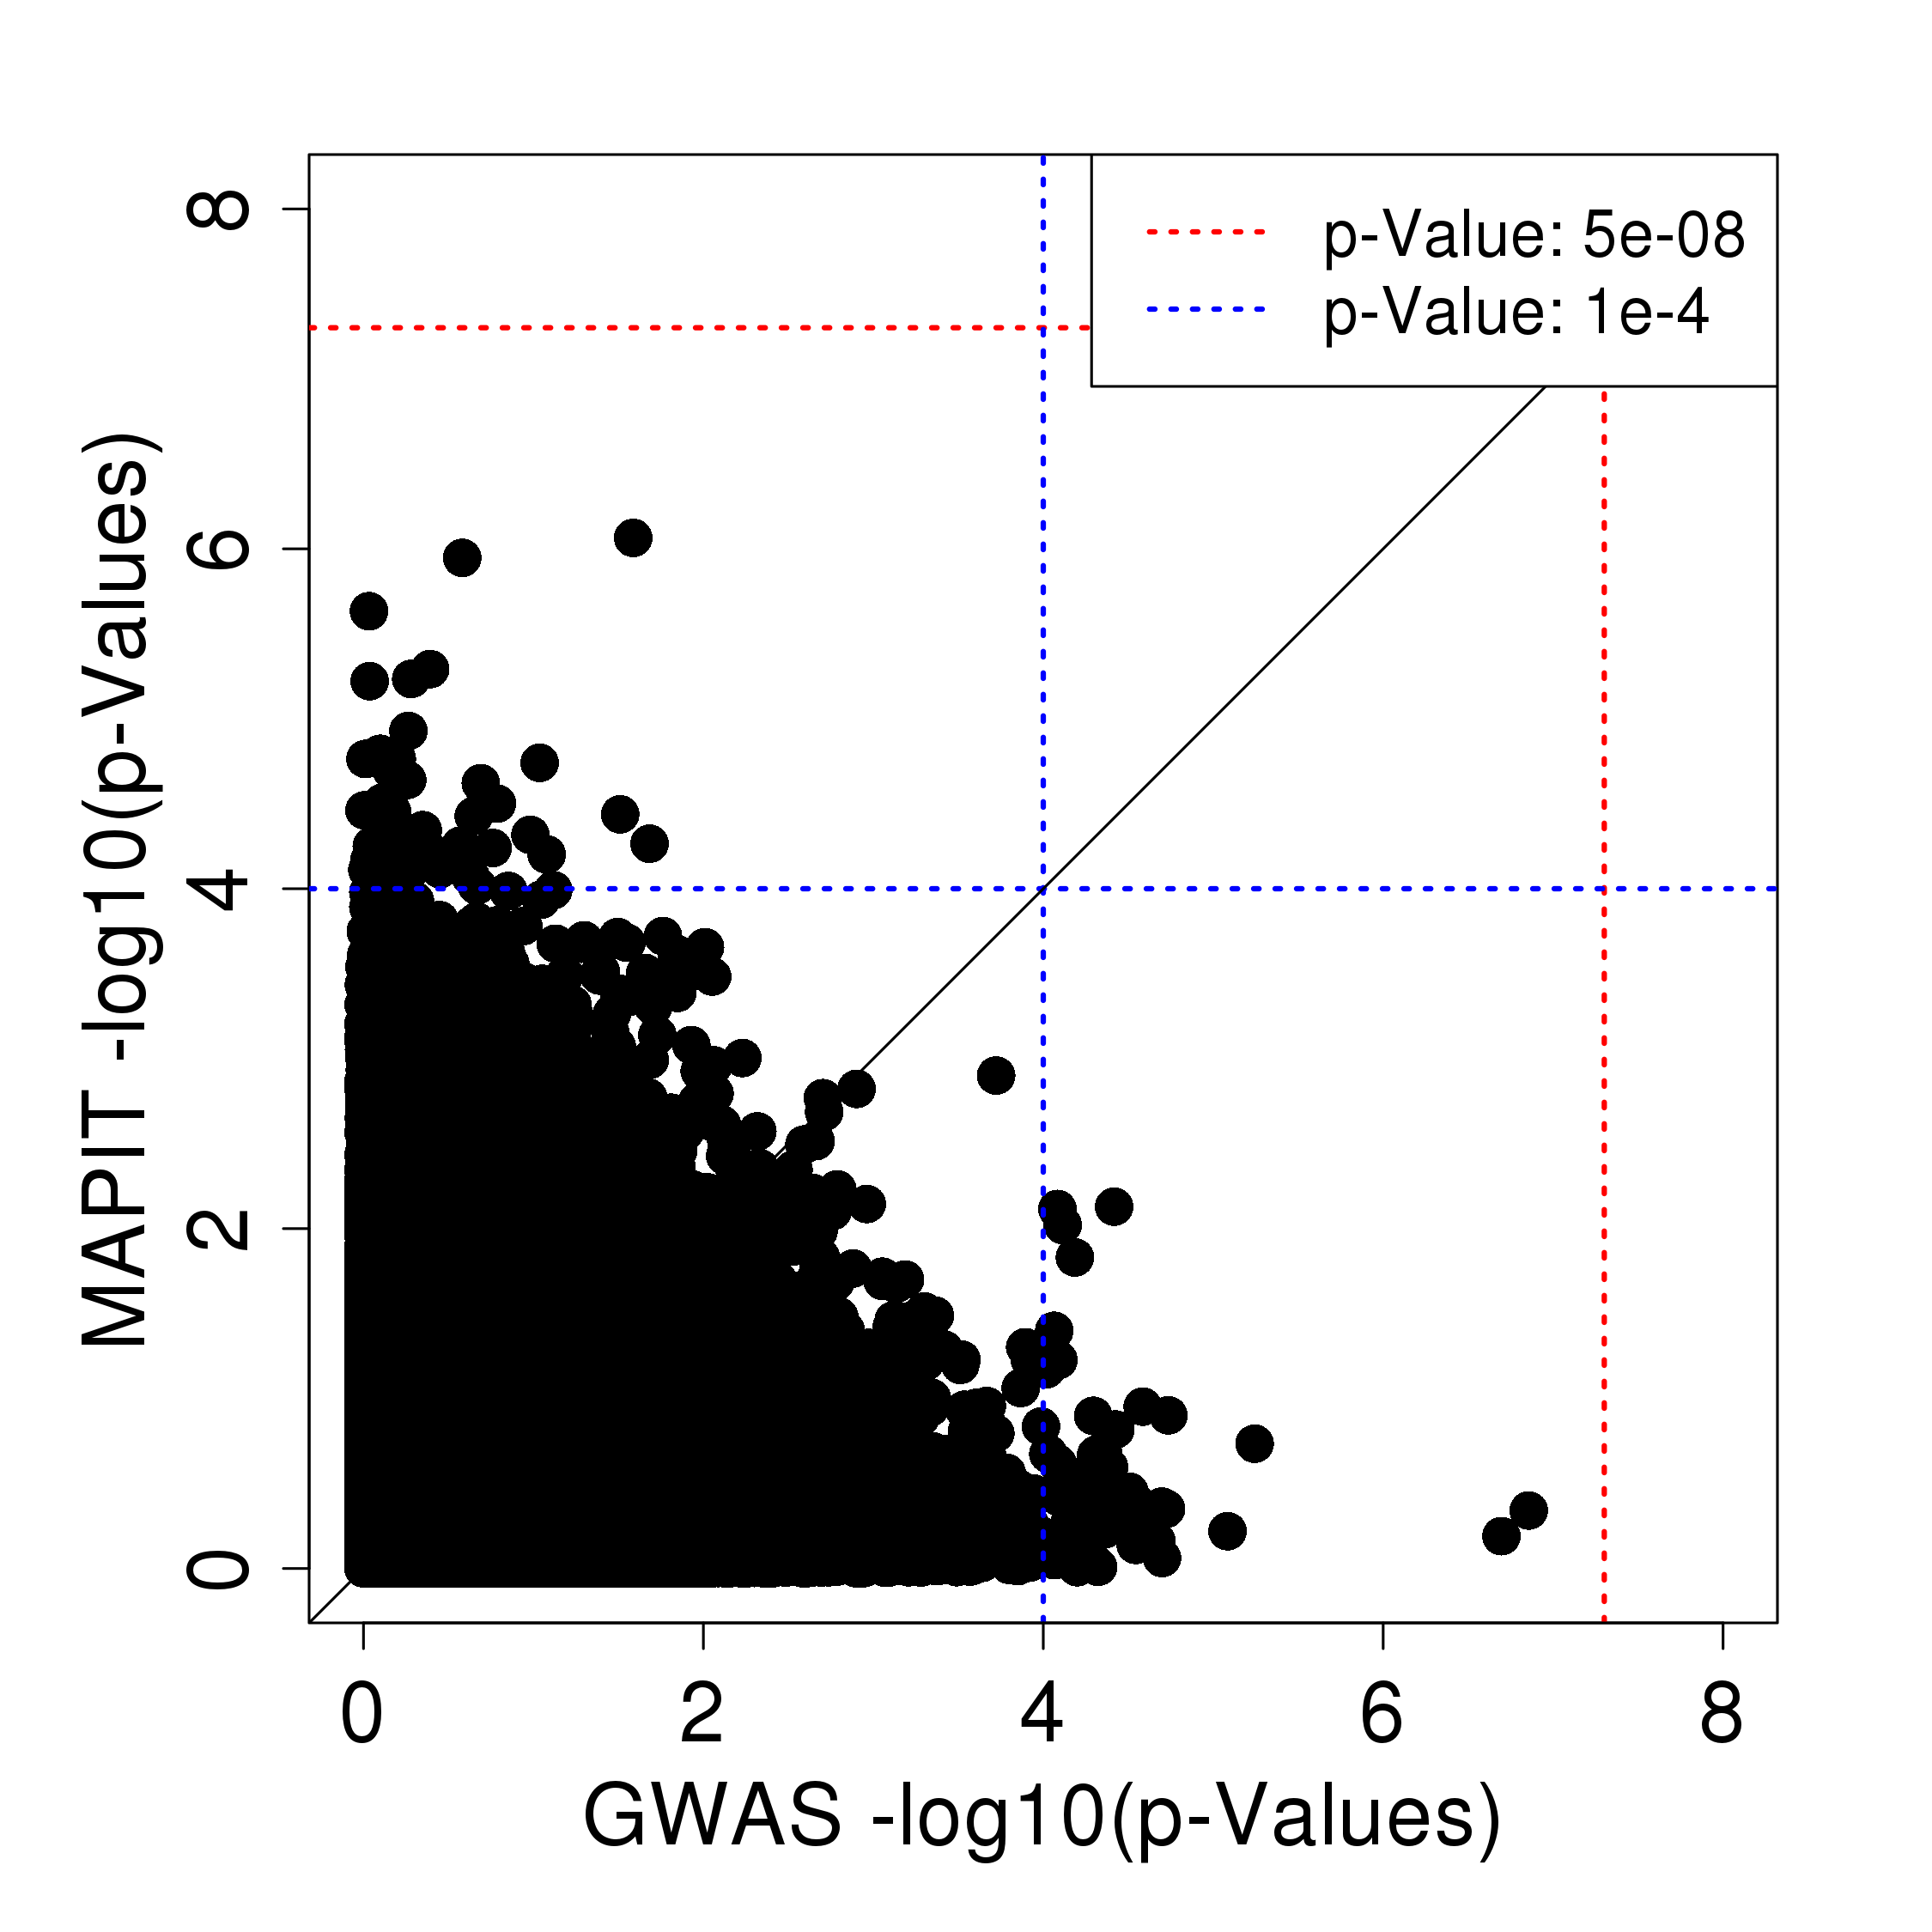
\includegraphics[scale=.35]{Images/Main/InterPath_Main_Figure_MAPITvsGWAS_vs2_AfrHght.png}
\caption[TBD]{\textbf{MAPIT vs. GWAS Results}.}
\label{InterPath-Main-Figure-MAPITvsGWAS-AfrHght}
\end{figure}

\textcolor{red}{(NOTE: below is what we were expecting for these results. But as you can see, the GIANT height/bmi results don't align in the way were anticipating. They are more spread out between height and BMI. I have checked though that the GIANT p-values of these top 500 SNPs are more correlated with our GWAS p-values than our MAPIT p-values (like ~.17 vs. .05). 
I think one alternative approach to this section is to angle instead as: 'we do not have power to even see a difference in GWAS vs. MAPIT as we were anticipating, thus indicating our real need to increase power. Hence, we moved forward with a method that we believed was going to accomplish that').}

To help further get a sense of whether these results are revealing patterns in true biology, we also annotated the top 500 SNPs with the most significant height and BMI GWAS $p$-values from the 2018 GIANT and UKB meta-analysis \cite{Yengo2018} in both our GWAS and MAPIT results. As expected, these 500 SNPs are heavily represented among the tail end of the most significant GWAS results, but maybe less expected is just how insignificant these SNPs appear on the MAPIT list of top results (\textcolor{red}{Supplementary Table -- listing differences in ranking of these 500 SNPs between GWAS and MAPIT}). In fact looking across the genome it is easy to see how different the relative ranking of SNPs are between the GWAS and MAPIT results (Figures \ref{InterPath-Main-Figure-MAPITvsGWAS-Manhattan}D \& \ref{InterPath-Main-Figure-MAPITvsGWAS-Manhattan}E). It is clear that even with our limited sample sizes, differences in the trends of importance of additive versus epistatic signals can be observed among marginally significant SNPs.  

\begin{figure}[htbp]
\centering
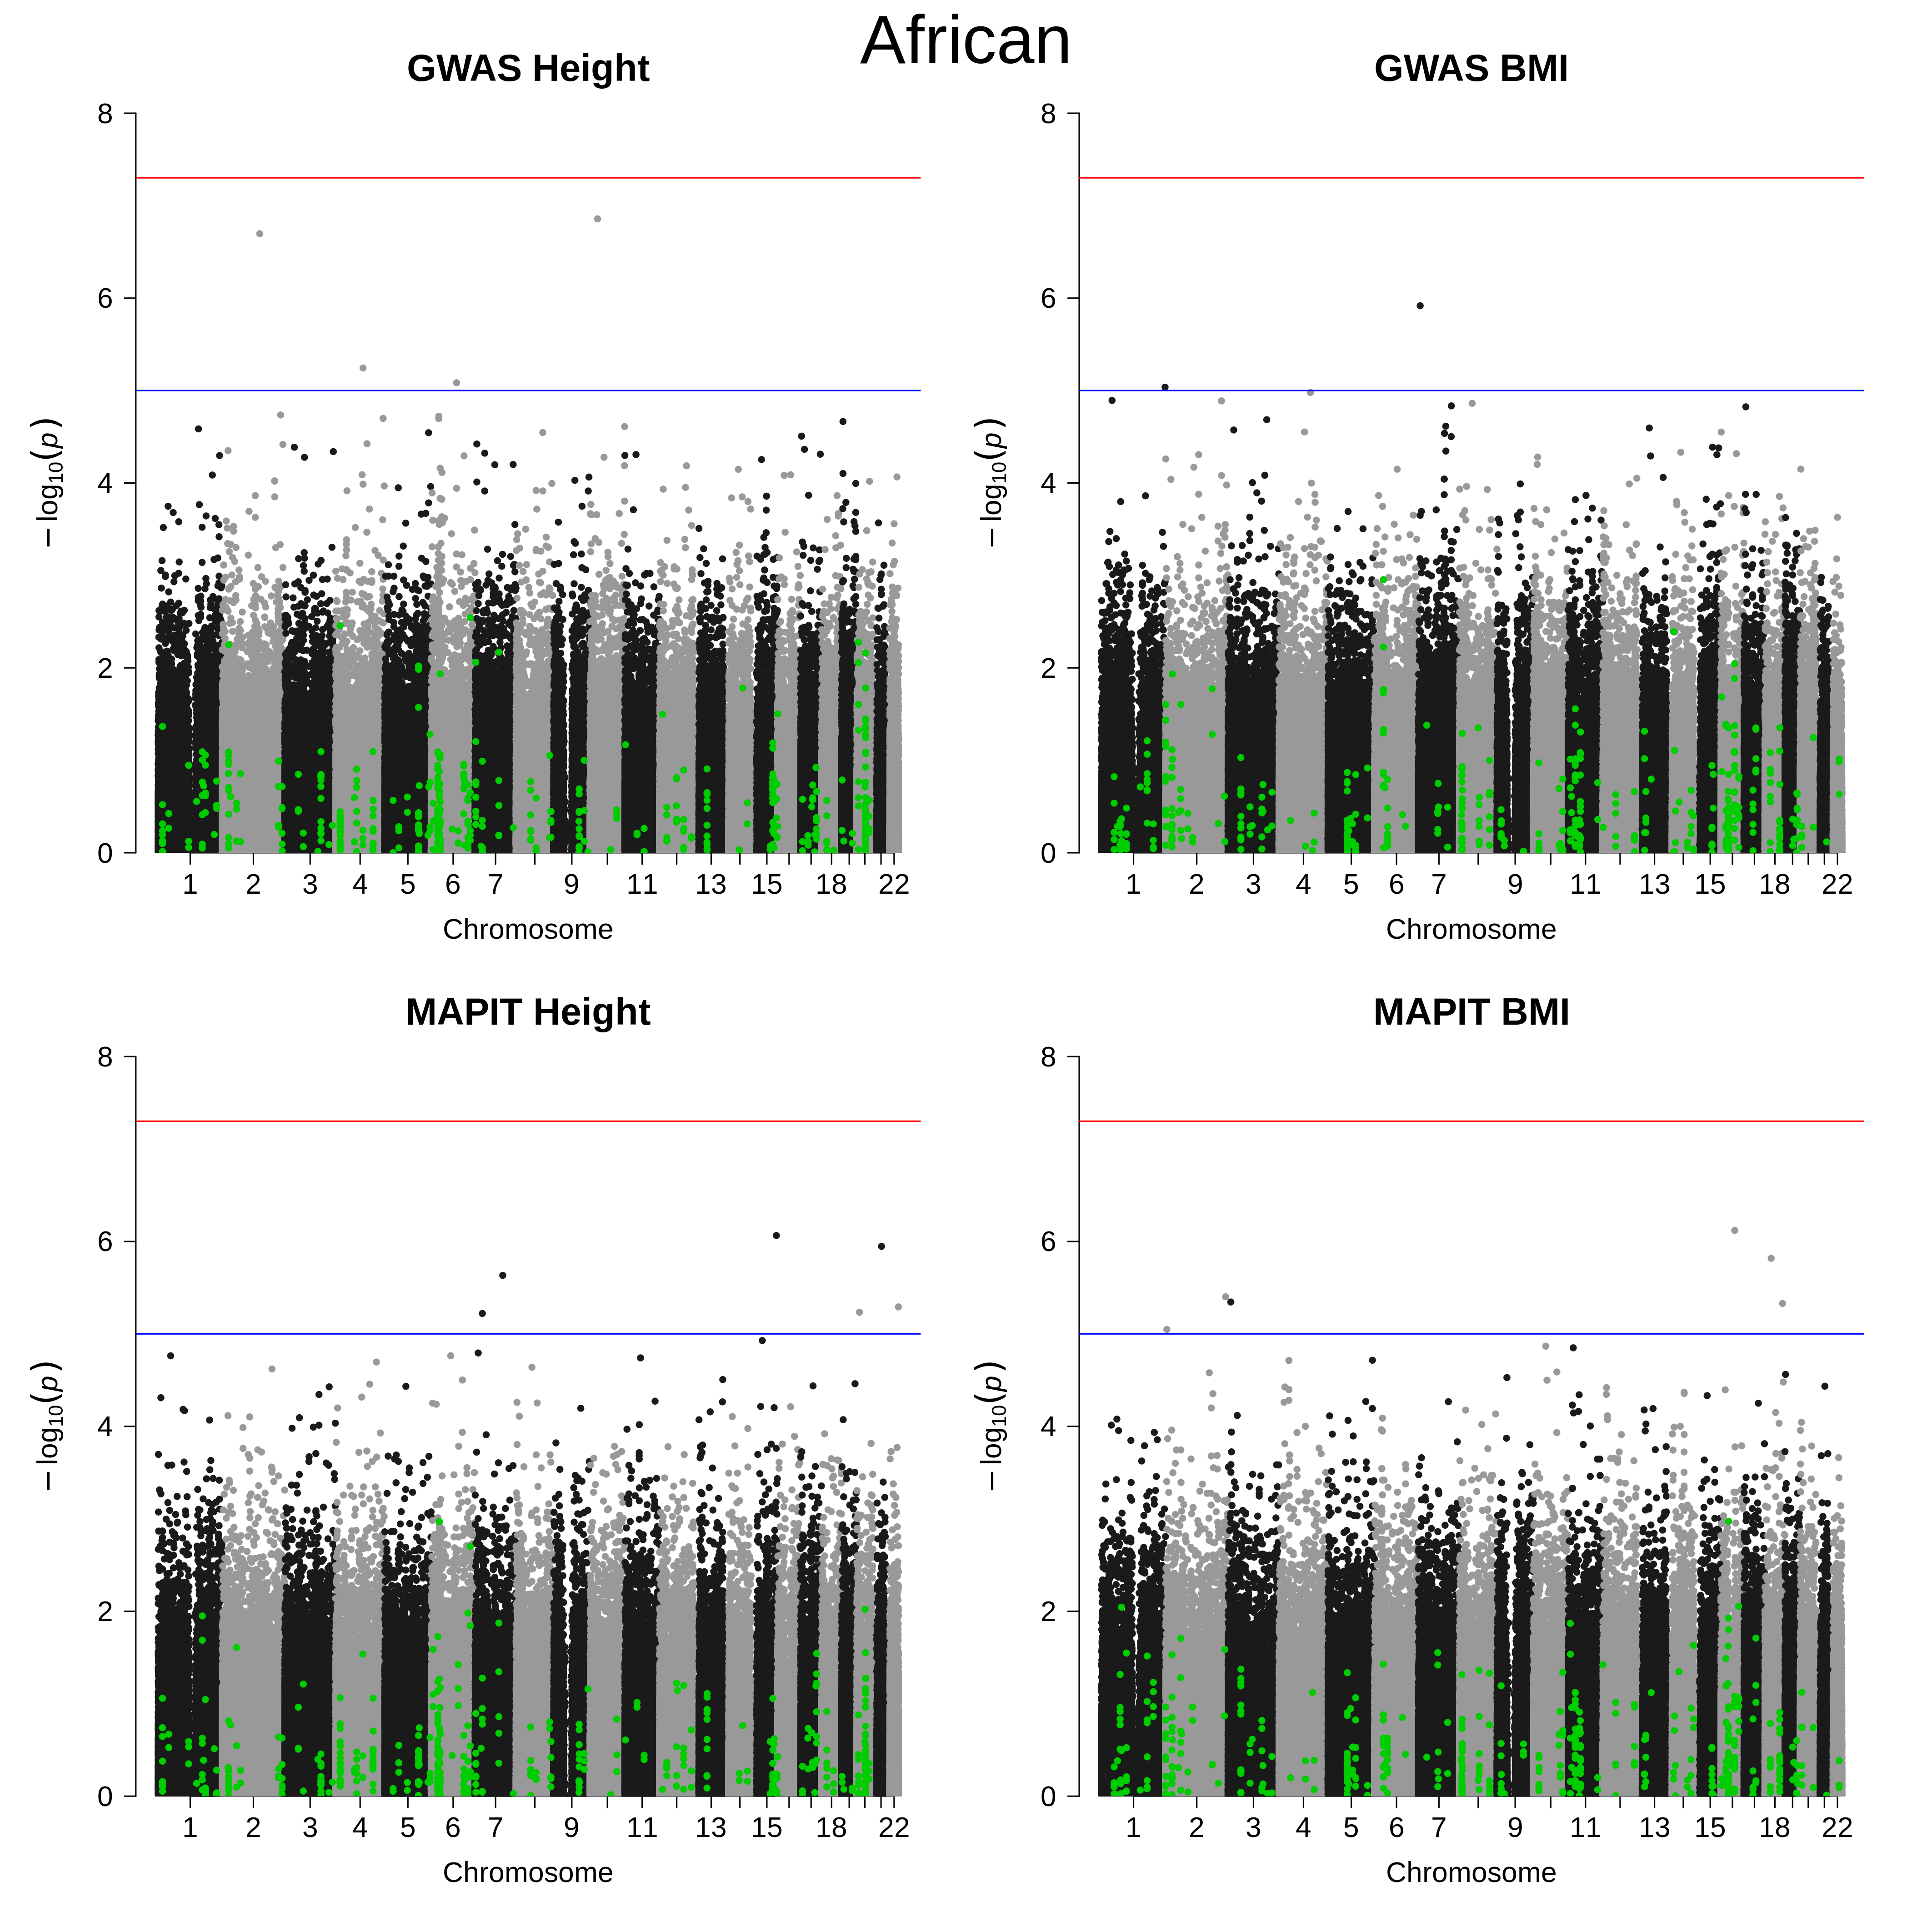
\includegraphics[scale=.35]{Images/Main/InterPath_Main_Figure_MAPITvsGWAS_Manhattan_vs1.png}
\caption[TBD]{\textbf{MAPIT \& GWAS Manhattan Plots}. \textcolor{red}{will be just height, MAPIT on top (D), GWAS on bottom (E), each plot wider. Green dots are the 500 SNPs that have the most significant GIANT/UKB p-values.}}
\label{InterPath-Main-Figure-MAPITvsGWAS-Manhattan}
\end{figure}

%\begin{figure}[htbp]
%\centering
%\includegraphics[scale=.35]{Images/Main/InterPath_Main_Figure_GWAS_Manhattan_vs1.png}
%\caption[TBD]{\textbf{GWAS Manhattan Plot}.}
%\label{InterPath-Main-Figure-GWAS-Manhattan}
%\end{figure}


\begin{align}
    & \textbf{y} = \mu + \textbf{R} + \textbf{G} + \textbf{Q} + \boldsymbol{\epsilon} \\
    \textbf{R} \sim \mathcal{MVN}&(\textbf{0}, \phi^{2}\textbf{K}_R) \quad \textbf{G} \sim \mathcal{MVN}(\textbf{0}, \omega^{2}\textbf{K}_G) \nonumber \\ 
    \textbf{Q} \sim \mathcal{MVN}&(\textbf{0}, \sigma^{2}\textbf{K}_Q) \quad \boldsymbol{\epsilon} \sim \mathcal{MVN}(\textbf{0}, \tau^{2}\textbf{I}) \nonumber 
\end{align}
where now R is a new random effects term that represents our new group of SNPs R, with variance component $\phi$ and GRM $\textbf{K}_R$ based on the SNP set R, and where now $\textbf{K}_Q = \textbf{K}_R \circ \textbf{K}_G$, the Hadamard product between the GRMs constructed from R and G. Similar to the MAPIT model, we construct our 'epistasis' random effect by conducting pairwise multiplication, though now it is between two matrices instead of a vector and a matrix. To see how this changes the additive form of the model, see equation XX in Materials and Methods. We fit this model similarly to before (also see Materials and Methods), and are interested in whether the variance component term $\sigma$ is significantly greater than 0.


Beyond extending our marginal epistasis model, we also expanded the number of UKB data subsets we analyzed given our encouraging results at the single SNP level. Specifically, we added UKB subsets consisting of Chinese, Pakistani, and Irish ancestry, as well as a second random subset of British individuals representing a larger sample size of close to 10,000 individuals. Both the Irish and new, second British subsets represent large sample size subsets to test how our model performs as sample size increases. Lastly, we chose to analyze the KEGG and REACTOME pathways available from the MSigDB \citep{Liberzon2011} due to their coverage of a wide range of biological processes. 




\subsection{GEMMA Analyses}

 the following variance component model:
\begin{equation}\label{InterPath-GEMMA-Equation-Model}
 \textbf{y} = \textbf{G}_1 + \textbf{G}_2 + \boldsymbol{\epsilon}
\end{equation}
where $y$ is a $n \times 1$ vector of phenotypes, $G_1$ is a $n \times n$ genetic relatedness matrix (GRM), constructed using all SNPs genome-wide and representing all first-order interactions, $G_2$ is a $n \times n$ matrix produced from the Hadamard product of $G_1$ against itself ($G_2 = G_1 \circ G_1$), representing all second-order interactions, and $\epsilon$ is a $n \times 1$ vector of normally distributed random effects. In other words, $G_1$ can be thought of as representing all additive effects, and $G_2$ can be thought of as representing all pairwise epistatic effects. To fit this model and estimate $G_2$, we used GEMMA \citep{Zhou2012} and its REML AI algorithm for estimating variance components.

GEMMA/GridLMM analyses were conducted using...







prev abstract

Genome-wide association (GWA) studies have identified thousands of significant genetic associations in humans across a number of complex traits. However, the vast majority of these studies use datasets of predominantly European ancestry \citep{Popejoy2016}. It has generally been thought that complex trait genetic architecture should be transferable across populations of different ancestries, but recent work has shown a number of differences in trait architecture across human ancestries, including heterogeneity in both the identified causal variants and estimated effect sizes 
\citep{Martin2017a,Wojcik2019}. Here, we report further evidence that complex trait genetic architecture is fundamentally different among human ancestries by jointly leveraging pathway and epistasis analysis.

Under the assumption that a given complex trait may have differential polygenic architectures across human ancestries, we hypothesize that human populations may also be enriched for differences in epistatic effects. However, since polygenic traits tend to have smaller GWA effect sizes, combining variants via pathway analysis may allow us to better reveal these \red{epistatic?} signals. To accomplish this, we extend the concept of identifying marginal epistasis, moving from testing single variants \citep{Crawford2017a} to testing groups of variants for nonlinear association with a trait of interest.

We apply our new method to multiple ancestries present in the UK Biobank \citep{Sudlow2015} and explore multiple pathway-related interaction models. Using morphometric traits we find evidence for genome-wide epistasis in African and other non-European populations. We also find evidence that these trends exists on the SNP and gene levels as well. Results also indicate this may be due to increased heterozygosity in non-European populations. This suggests that non-European populations may be well-suited for identifying non-additive effects in human complex trait architecture; this also suggests further evidence that European populations -- predominantly used for epistasis studies -- may indeed be limited and inaccurate proxies for all human ancestries in complex trait research.

sample size scaling issue. multiple testing setup? looking at better searching algorithm? gridd?

one possible avenue of future research is the use of summary statistics for epistatic analyses, similar to other recent methodological extensions to include GWAS summary statistics (matthew, bmass, one or two others?).









And the PLINK model is as follows:
\begin{equation}
\textbf{y} = \beta_0 + \textbf{x}_1\beta_1 + \textbf{x}_2\beta_2 + \textbf{x}_1*\textbf{x}_2\beta_3    
\end{equation}
where \textbf{y} is once again a $n \times 1$ vector of phenotypes, $\beta_0$ is the y-intercept, $\textbf{x}_1$ is a $n \times 1$ vector of genotypes for SNP 1, $\beta_1$ is the corresponding additive effect size for $\textbf{x}_1$, $\textbf{x}_2$ is a $n \times 1$ vector of genotypes for SNP 2, $\beta_2$ is the corresponding additive effect size for $\textbf{x}_2$, $\textbf{x}_1 * \textbf{x}_2$ is the multiplicative interaction between $\textbf{x}_1$ and $\textbf{x}_2$, and $\beta_3$ is the corresponding effect size for $\textbf{x}_1 * \textbf{x}_2$. Our variable of interest of course is $\beta_3$ and whether this value significantly deviates from 0.


To test for SNP-level marginal epistasis, we use MAPIT \citep{Crawford2017a}. For a full derivation of the MAPIT framework please see \citet{Crawford2017a}, but in short MAPIT begins with the following setup:
\begin{equation}
\textbf{y} = \mu + \textbf{x}_k\beta_k + \sum_{l \neq k} \textbf{x}_l\beta_l + \sum_{l \neq k} (\textbf{x}_k \circ \textbf{x}_l)\alpha_l + \boldsymbol{\epsilon}, \quad \boldsymbol{\epsilon} \sim \mathcal{MVN}(\textbf{0}, \tau^{2}\textbf{I})  
\end{equation}

where \textbf{y} is still a $n \times 1$ vector of phenotypes, $\textbf{x}_k$ is a $n \times 1$ vector of genotypes for our SNP of interest $k$, $\beta_k$ is our additive effect size for SNP $k$, $\textbf{x}_l$ is a $n \times 1$ vector of genotypes for every SNP $l$ that is not SNP $k$, $\beta_l$ is our additive effect size for SNP $l$, $(\textbf{x}_k \circ \textbf{x}_l)$ is the Hadamard product between our two SNP genotype vectors, $\alpha_l$ is interaction effect size, $\boldsymbol{\epsilon}$ is a $n \times 1$ vector of random effects which follow a multivariate normal distribution with mean $\textbf{0}$ and covariance matrix equal to variance effect $\tau$ times the $n \times n$ identity matrix $\textbf{I}$. In this model our parameter of interest would be $\alpha_l$, whether there is any significant interaction between our SNP of interest $k$ and of the remaining SNPs in the genome. However, as one might expect, the number of parameters in this model far exceeds the number of samples (ie $p >> n$), therefore making the solution indeterminable. To overcome this, MAPIT moves this setup into a linear mixed model framework and make the problem a variance component one. To do this, we put normal random priors on each of our effect sizes ($\beta_k$, $\beta_l$, and $\alpha_l$), and redefine our model as follows:
\begin{align}
    & \textbf{y} = \mu + \textbf{x}_k\beta_k + \textbf{m}_k + \textbf{g}_k + \boldsymbol{\epsilon} \\
    \textbf{m}_k \sim \mathcal{MVN}(\textbf{0}, &\omega^{2}\textbf{K}_k) \quad \textbf{g}_k \sim \mathcal{MVN}(\textbf{0}, \sigma^{2}\textbf{G}_k) \quad \boldsymbol{\epsilon} \sim \mathcal{MVN}(\textbf{0}, \tau^{2}\textbf{I}) \nonumber 
\end{align}
where $\textbf{m}_k$ and $\textbf{g}_k$ are both random effects that follow multivariate normal distributions, $\omega$ and $\sigma$ are their respective variance components, $\textbf{K}_k = \textbf{X}_{-k}\textbf{X}^{\textbf{T}}_{-k}/(p-1)$, the genetic relatedness matrix (GRM) constructed from all SNPs available aside from SNP $k$, and $\textbf{G} = \textbf{D}_k\textbf{K}_k\textbf{D}_k$, a GRM based on pairwise interaction terms between the $k$\textsuperscript{th} variant and all other variants. Here, we denote $\textbf{D}_k =$ diag$(\textbf{x}_k)$ to be an $n \times n$ diagonal matrix with the genotype vector $\textbf{x}_k$ as its diagonal elements. Our parameter of interest here is $\sigma$ and whether it is significantly larger from 0; a significant deviation would represent there exist some subset of genetic interactions between $k$ and the rest of the genome.








It has generally been thought that complex trait genetic architecture should be transferable across populations of different ancestries, but recent work has shown a number of differences in additive trait architecture across human ancestries, including heterogeneity in both the identified causal variants and estimated effect sizes. Here, we explore a form of non-additive trait architecture, epistasis, to see if there are similar discrepancies in complex trait association metrics across ancestries in a diverse dataset.







The second of these two situations is what we tried to resolve first. If we are concerned about a relationship between larger pathways and inflated hypergeometric $p$-values, then one possible approach might be to restrict the size of the pathways analyzed. Instead of looking at enrichment among all pathways, we can instead look at enrichment only among pathways that have under a certain number of SNPs. And indeed, by restricting the number of SNPs present in a pathway to 1,000 or less, we see a major drop off in the number of significant pathways remaining (29 to 2 for KEGG height, 47 to 11 for KEGG BMI, 24 to 0 for REACTOME height, and 65 to 26 for REACTOME BMI); this, by extension, also produces a large drop in the genes that are present across these pathways as well as their associated hypergeometric $p$-values (Supplementary Figure \ref{InterPath-Supp-Figure-Hypergeometric-RestrictedComps-African-BMI} and Supplementary Table \ref{InterPath-Supp-Table-Hypergeometric-RestrictedComps-African-BMI-TopExamples}). Interestingly however, we find one gene family that has had the opposite result -- multiple proteasome subunit genes (\textit{PSMA}*, \textit{PSMB}*, \textit{PSMC}*, \textit{PSMD}*, and \textit{PSME*}) now produce more significant hypergeometric $p$-values upon this restriction to pathways with smaller SNP counts (Supplementary Table \ref{InterPath-Supp-Table-AllPops-TopGeneCount-HypergeometricTests}). 





To identify possible biological mechanisms or processes enriched for epistatic interactions, we tested whether genes are overrepresented among the pathways we identified as having significant marginal epistasis signals genome-wide versus the background distribution of pathways in each database (KEGG and REACTOME). Supplementary Figure \ref{InterPath-Supp-Figure-Hypergeometric-QQPlots-African} lists genes significantly enriched among our significant MAPIT-R pathways using a hypergeometric test. 
In the African subgroup, we find an abundance of `significant' $p$-values for both height and BMI in both pathway databases. Using the Bonferroni cutoff of $2.082\times10^{-5}$ (.05 / 2401 genes), we would identify 45 genes as being significantly enriched in the REACTOME BMI analysis. We tested whether these results were confounded by pathway size (number of SNPs in the pathway; Supplementary Figure \ref{InterPath-Supp-Figure-pValsVsNumSNPs}), and we note that solely having more variants does not lead to smaller MAPIT-R $p$-values, as shown in the permuted phenotype analyses in Supplementary Figure \ref{InterPath-Supp-Figure-pValsVsNumSNPs-perm1}). As a result, this enrichment analysis may be moreso identifying genes that are overrepresented among larger pathways, such as housekeeping genes, than genes that are necessarily overrepresented among MAPIT-R significant pathways. 

To further test the effect of pathway size on our results, we conducted a second enrichment analysis restricted to pathways with less than 1,000 SNPs (Figure \ref{InterPath-Main-Figure-Hypergeometric-RestrictedComps-African-BMI}). This reduces the number of genes significantly enriched in pathways identified with significant marginal epistasis using MAPIT-R. However, in this restricted analysis, one gene and a separate gene family have enrichment $p$-values that have become more significant. The gene with the largest increase in significance is {\emph{SMC3}}, a component of the multimeric cohesin complex. The others genes that were identified as significantly enriched in MAPIT-R-identified pathways in the restricted analysis are all from the same family of proteins, the various subunits of the proteasome complex ({\emph{PSMA*}}, {\emph{PSMB*}}, {\emph{PSMC*}}, {\emph{PSMD*}}, {\emph{PSME*}}, and {\emph{PSMF*}}). The proteasome is one half of the ubiquitin-proteasome system (UPS), a critical system for a variety of processes related to protein degradation within the cell \citep{Voges1999,Livneh2016,Collins2017}. Whereas ubiquitin is the first half of this system that tags proteins for eventual degradation, the proteasome is the second half of this system that catalyzes the degradation itself. The main proteasome isoform, 26S, is made up of two main components: the 20S main core of four stack rings (an outer, structural ring encoded by PSMA genes, and an inner, catalytic ring encoded by PSMB genes) and the 19S regulatory caps which booked both sides of the main core (encoded by both PSMC and PSMD genes) (Figure \ref{InterPath-Main-Figure-Proteasome-Schematic}). 

\begin{figure}[htb]
\centering
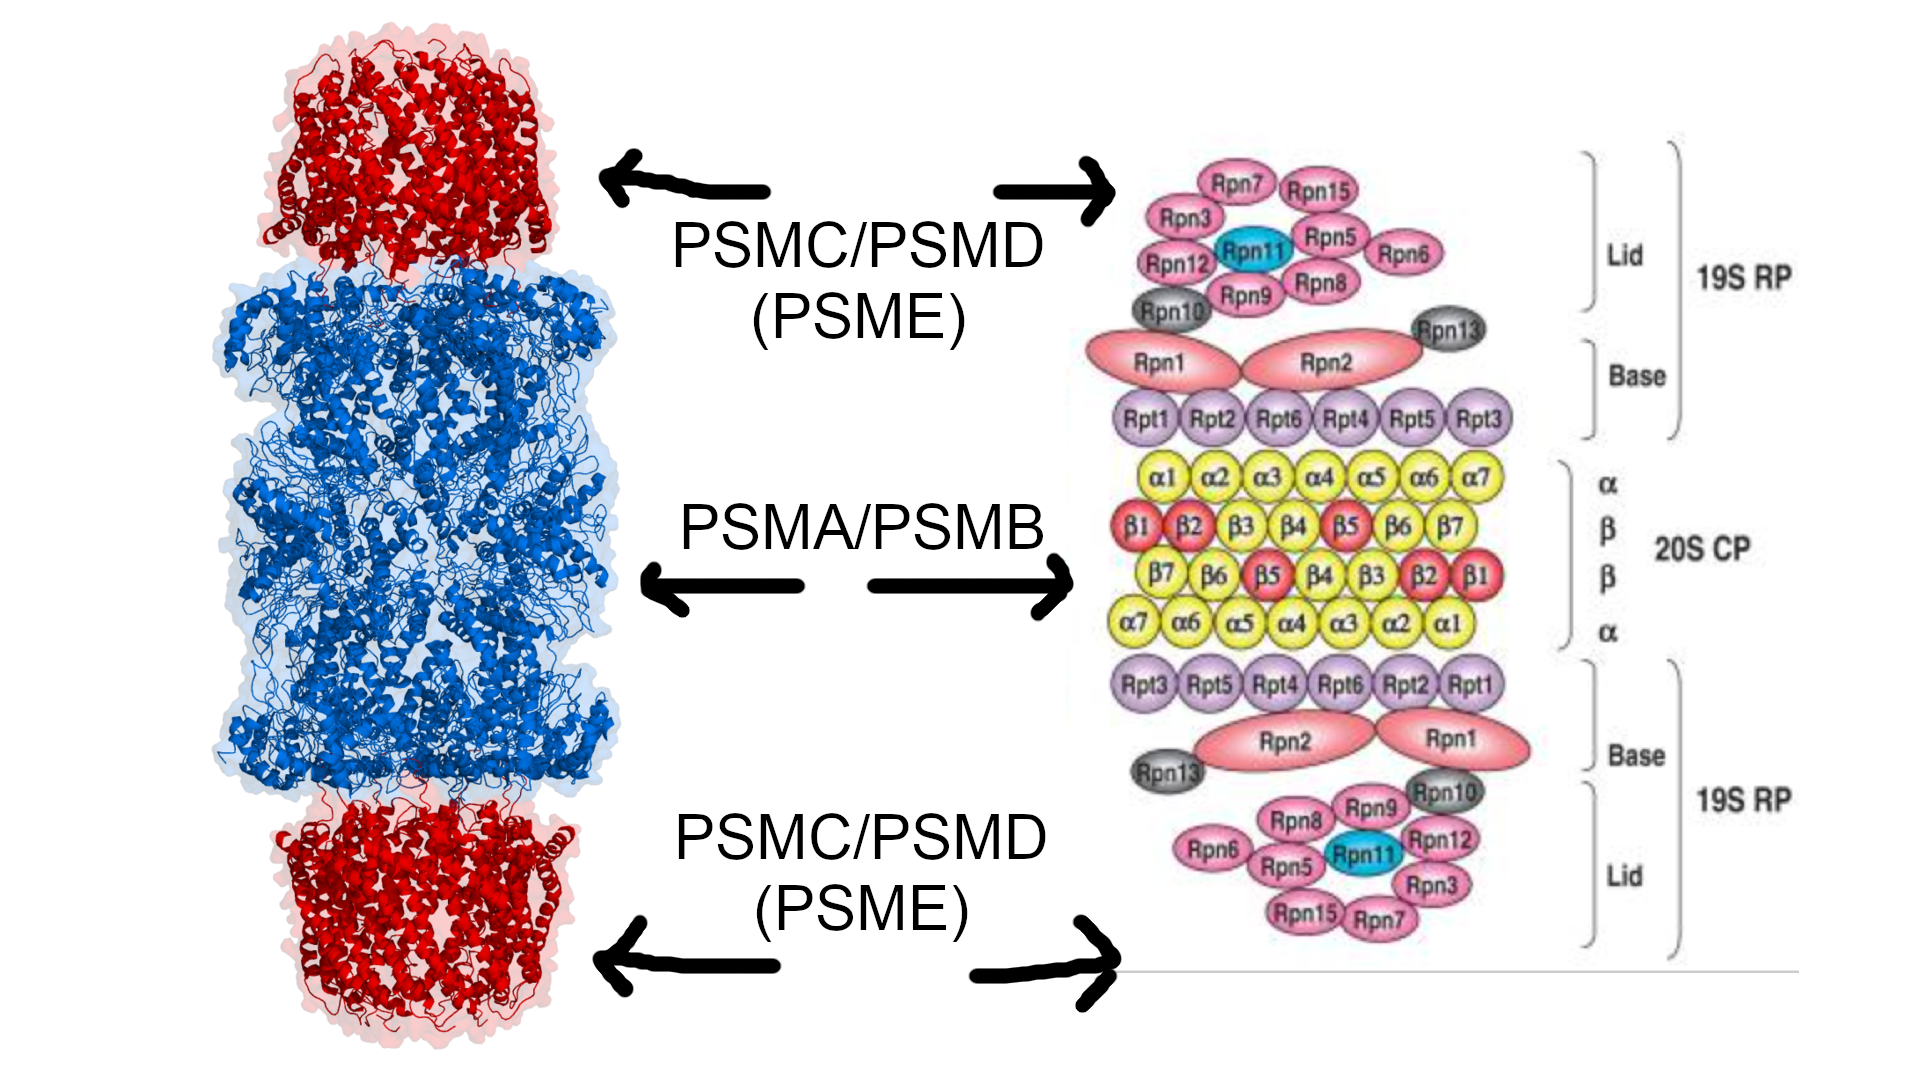
\includegraphics[scale=.2]{Images/Main/MockUp1.png}
\caption[TBD]{\textbf{Structure of the Proteasome}. The figure shows the different components of the proteasome and which gene families encode which part. \textcolor{blue}{MT: currently a mockup of an idea on how to present this -- maybe this and the heatplot should be one larger figure? } \textcolor{red}{SR: I think maybe you need to note more of your results here - like which genes were significant in which analysis using your results?}
}
\label{InterPath-Main-Figure-Proteasome-Schematic}
\end{figure}


\subsection{MAPIT-R identifies signals of epistasis in diverse UKB subgroups where pairwise tests for epistasis fail}\label{InterPath-Results-SNPEpistasis}

\textcolor{red}{SR: Next we wanted to test whether we could identify significant pairwise epistatic interactions between pairs of SNPs such that one SNP in the pair was in a pathway MAPIT-R identified as having genome-wide significant marginal epistasis with the rest of the genome. We were particularly interested in identifying epistatic interactions with pathways showing ancestry-specific signals of marginal epistasis in our MAPIT-R application (cite appropriate figure).} To this end, we applied MAPIT to each of our UKB subgroups for both height and BMI. We find that there are no SNPs with genome-wide significant signals for marginal epistasis ($p$-value $< 5\times10^{-8}$; Supplementary Figure \ref{InterPath-Supp-Figure-MAPIT-HeightBMI}). While we observe possible enrichment of marginally significant $p$-values ($p$-value $< 5\times10^{-4}$) in the African, Caribbean, and Indian subgroups versus the British, Chinese, and Pakistani subgroups in both phenotypes, it is not as clear a between-ancestry pattern as we observe in the MAPIT-R results. And to compare against the more typical, direct pairwise variant epistasis analysis, we also applied PLINK's exhaustive pairwise epistasis test \citep{Purcell2007} to each of our ancestry subgroups in height and BMI, and once again do not observe any genome-wide significant tests ($p$-value $\leq 5\times10^{-13}$, Bonferroni-corrected for $1\times10^{11}$ tests; Supplementary Figure \ref{InterPath-Supp-Figure-PLINK-HeightBMI-AllPops}).



\begin{figure}[htb]
\centering
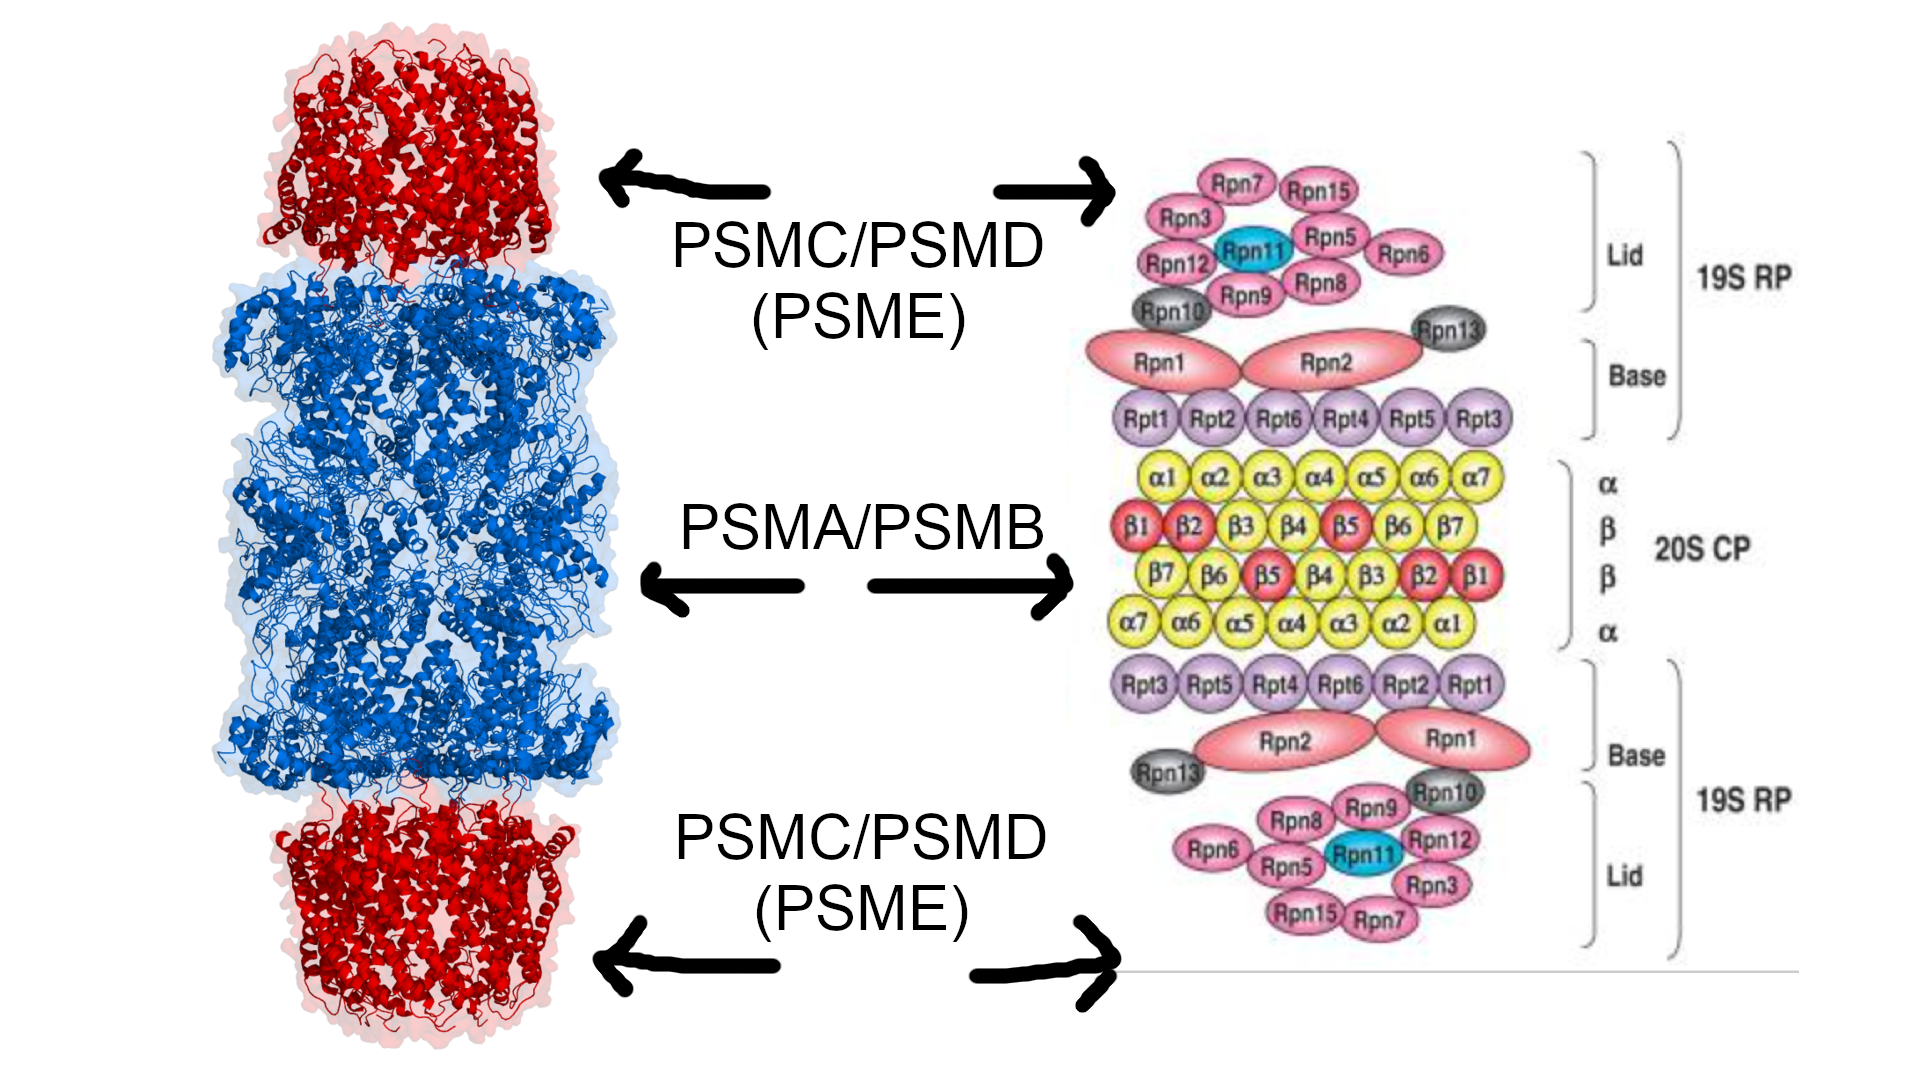
\includegraphics[scale=.2]{Images/Main/MockUp1.png}
\caption[TBD]{\textbf{Structure of the Proteasome}. The figure shows the different components of the proteasome and which gene families encode which part. \textcolor{blue}{MT: currently a mockup of an idea on how to present this -- maybe this and the heatplot should be one larger figure? } \textcolor{red}{SR: I think maybe you need to note more of your results here - like which genes were significant in which analysis using your results?}
}
\label{InterPath-Main-Figure-Proteasome-Schematic}
\end{figure}


\begin{figure}[]
\centering
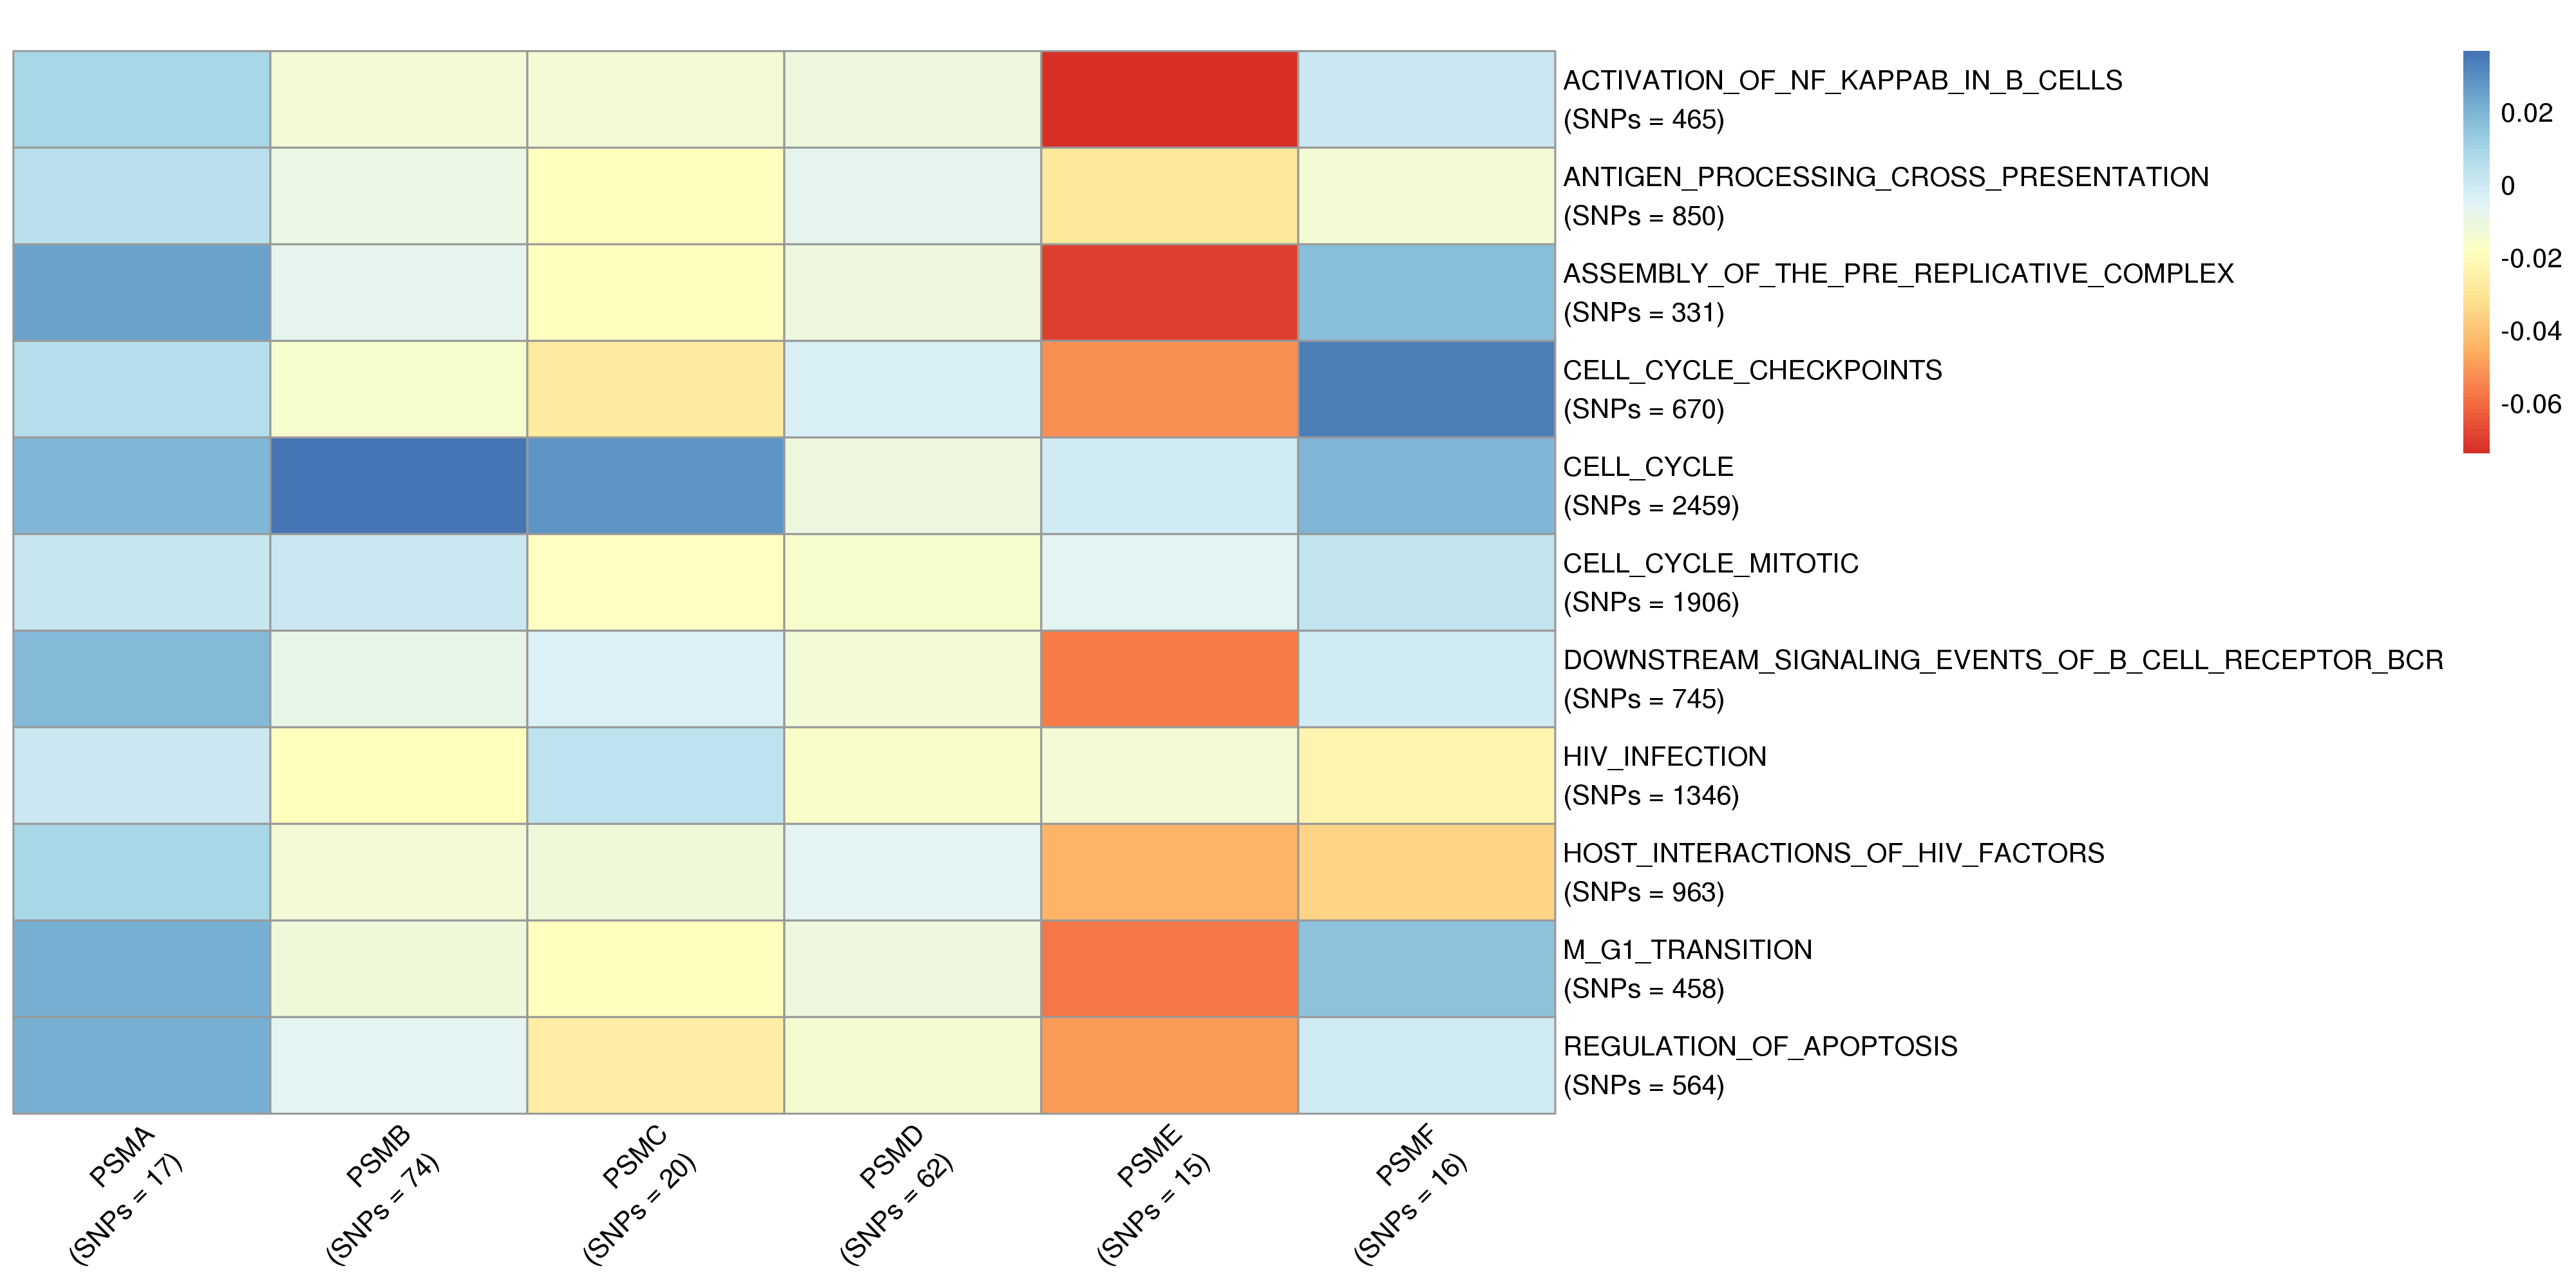
\includegraphics[scale=.45]{Images/Main/InterPath_Main_Figure_Proteasome_vs1.png}
\caption[TBD]{\textbf{Change in MAPIT-R $p$-values when removing proteasome subunits}. The figure shows the change in MAPIT-R $p$-value for each REACTOME pathway labeled when the SNPs in each proteasome subunit gene family are removed from the analysis. The heatplot shows the -$\log_{10}$ $p$-value change per SNP, with each column corrected for the number of SNPs in each subunit gene family. Two patterns of note are: removing the PSMA gene family does not significantly change the MAPIT-R $p$-values. PSMA genes also encode for the outer structural rings of the 20S structure and do not have any known catalytic activity, supporting they may have less important genetic interactions. Second, the PSME gene family appears to have particularly strong effects on pathways related to NF$\kappa$B, B-cells, HIV-infection, and apoptosis. PSME genes encode an alternative regulatory particle (11S or PA28) that can form hybrid-proteasome structures that are known to enhance production of a specific subclass of MHC-1 antigens in a ubiquitin-independent manner, and recent work has connected PSME genes to upregulation of NF$\kappa$B. Therefore PSME genes may have a different and stronger set of genetic interactions within these pathways as compared to the other subunit gene families, which is getting represented here.
}
\label{InterPath-Main-Figure-Proteasome-Heatplot}
\end{figure}



%Focusing on pathways with the largest number of SNPs, and therefore potentially the pathways with the largest signals, we do see a marginally significant relationship in the African subgroup using REACTOME pathways (Figure \ref{InterPath-Main-Figure-PC1Loading}; linear regression $p$-value $\approx$ .05), but this result is not replicated in the KEGG pathways. Overall then, it is still unclear if and how within-subgroup genetic variation relates back to the differences between subgroup MAPIT-R results we observe.

%\begin{figure}[htb]
%\centering
%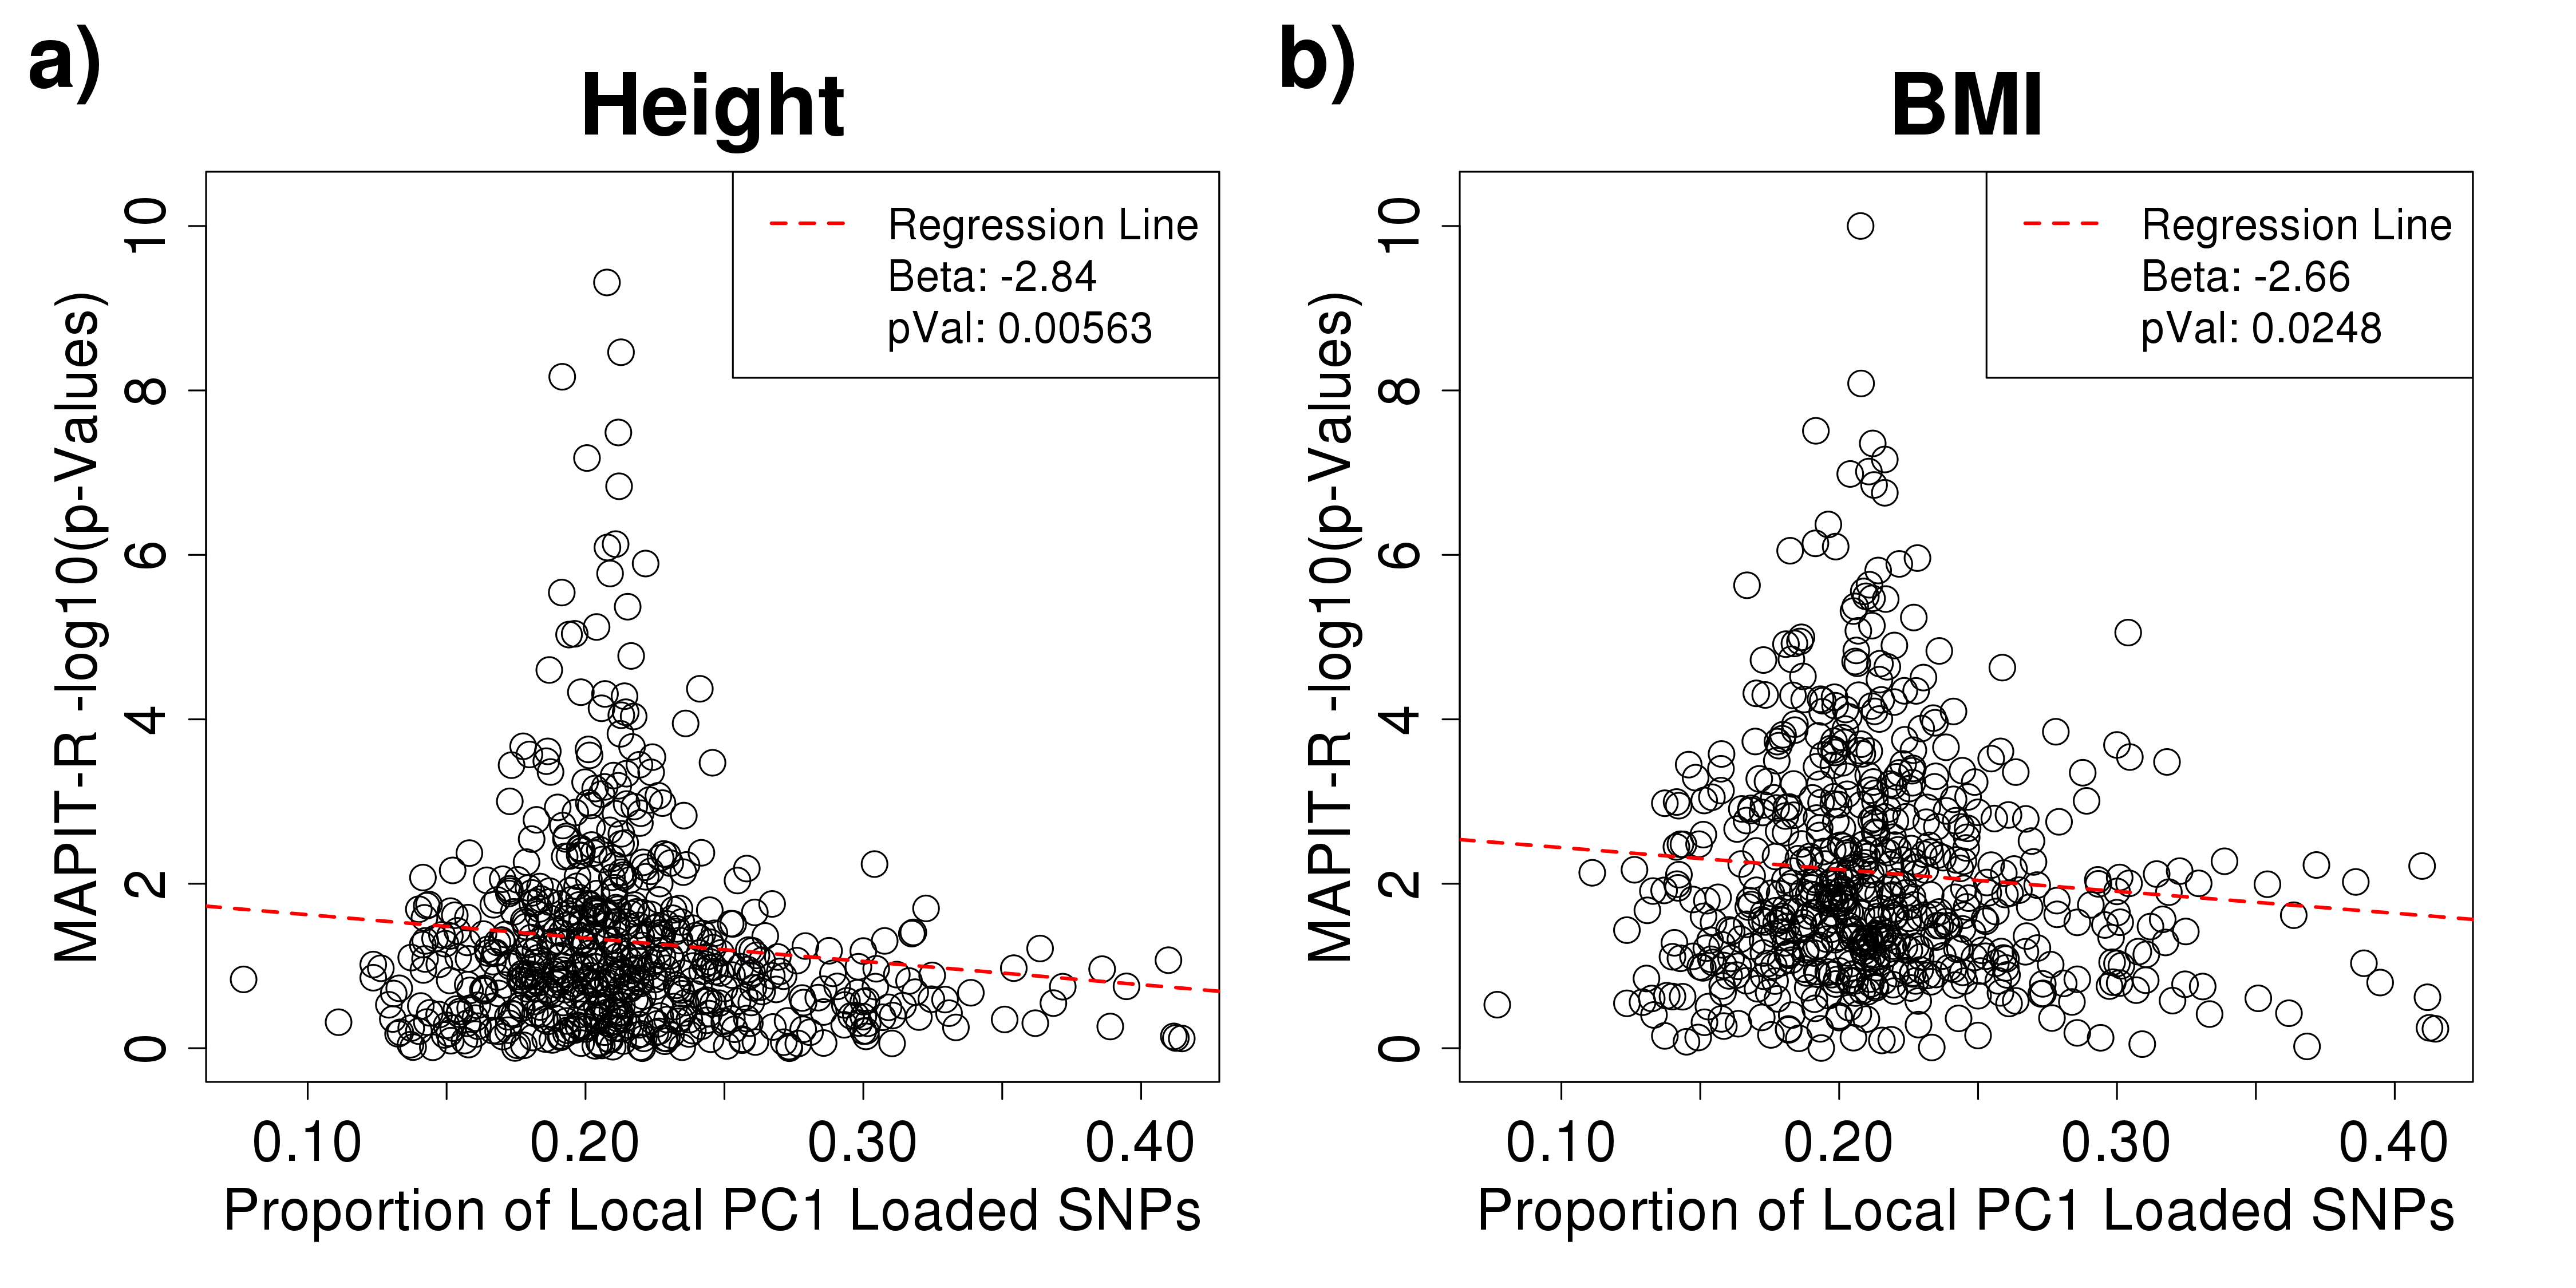
\includegraphics[scale=.35]{Images/Main/InterPath_Main_Figure_PC1Loading_vs2_noHLA.png}
%\caption[TBD]{\textbf{Relationship between MAPIT-R $p$-values and proportions of pathway SNPs loaded on PC1, African subgroup and large pathways}. The figure shows the proportion of SNPs within a given pathway that are strongly loaded on local PC1 plotted against that pathway's MAPIT-R -$\log_{10}$ $p$-value, specifically for the African subgroup and in the (a) KEGG and (b) REACTOME pathway databases. `Local' here refers to PCA having been conducted within-subgroup. SNPs are designated as `strongly loaded' on local PC1 if they are within the 10\% tails of the loading SNP score distributions. We observe that there is no significant relationship between MAPIT-R $p$-values and proportion of SNPs that are strongly loaded on PC1 in either pathway database, and for the majority of analyses done in the other subgroups \ref{InterPath-Supp-Figure-PC1Loading-AllPaths}.}
%\label{InterPath-Main-Figure-PC1Loading}
%\end{figure}


However, looking at within subgroup F\textsubscript{ST} (the diagonal)\footnote{\textcolor{blue}{MT: note, this is predicated on using a proper metric for the diagonal; if we one doesn't come up, or if it doesn't match the following descriptions, I'll update things to match and follow the figure properly}}, we observe that the African subgroup has the largest amount of differentiation as compared to any other subgroup. Additionally, the Caribbean and Chinese subgroups are the subgroups with the next largest values of within subgroup F\textsubscript{ST}, approximately matching the order in which subgroups produce significant pathway MAPIT-R results. Next we tested whether within-subgroup levels of genetic variation were associated with more significant signals of marginal epistasis in MAPIT-R analyses.


into which regions of the genome . 

we also examined whether cryptic population structure within subgroups was associated with increased signals of marginal epistasis in our MAPIT-R analyses. Specifically, we investigated correlations between the percent variance explained by within-subgroup principal components (Figure \ref{InterPath-Main-Figure-Eigenvalues} with the number of genome-wide MAPIT-R results we found per subgroup. And indeed, similar to the within-subgroup F\textsubscript{ST} values we saw, we find that subgroup PVE on PC1 matches an order similar to which populations produce the largest numbers of significant pathways.

\subsection{PLINK Analyses}

PLINK pairwise epistasis analyses were conducted using PLINK v1.90b4 \citep{Purcell2007}, the `\texttt{-{}-epistasis}' command, and phenotypes that had top 10 local PCs regressed out; PCs were regressed out directly from the phenotypes due to the `\texttt{-{}-epistasis}' function having no explicit form to incorporate covariates. Default values for the `\texttt{-{}-epi1}' and `\texttt{-{}-epi2}' options (0.0001 and 0.01, respectively) were kept.   

\subsection{MAPIT Analyses}

MAPIT analyses were conducted using the MAPIT software downloaded from \url{https://github.com/lorinanthony/MAPIT}. MAPIT was run using the phenotypes as previously described and top 10 local PCs as covariates. Specifically, we used the `\texttt{MAPIT\_Davies\_Approx}' function due to its computational speed up and because our datasets had large enough sample sizes to properly employ the approximate form.  




\fi

\end{document}
